\chapter{The Fisher Matrix: Forecasting What Data Can Teach}\label{ch:10}
\providecommand{\TenACowFaa}{}\renewcommand{\TenACowFaa}{450}
\providecommand{\TenACowFab}{}\renewcommand{\TenACowFab}{-90}
\providecommand{\TenACowFbb}{}\renewcommand{\TenACowFbb}{99}
\providecommand{\TenACowIaa}{}\renewcommand{\TenACowIaa}{0.2250}
\providecommand{\TenACowIab}{}\renewcommand{\TenACowIab}{-0.0451}
\providecommand{\TenACowIbb}{}\renewcommand{\TenACowIbb}{0.0497}
\providecommand{\TenACowSa}{}\renewcommand{\TenACowSa}{0.052}
\providecommand{\TenACowSb}{}\renewcommand{\TenACowSb}{0.111}
\providecommand{\TenACowRho}{}\renewcommand{\TenACowRho}{0.43}
\providecommand{\TenACowCondA}{}\renewcommand{\TenACowCondA}{0.047}
\providecommand{\TenACowCondB}{}\renewcommand{\TenACowCondB}{0.100}
\providecommand{\TenACowMSa}{}\renewcommand{\TenACowMSa}{0.050}
\providecommand{\TenACowMSb}{}\renewcommand{\TenACowMSb}{0.108}
\providecommand{\TenACowMRho}{}\renewcommand{\TenACowMRho}{0.44}
\providecommand{\TenACowMeanA}{}\renewcommand{\TenACowMeanA}{0.498}
\providecommand{\TenACowMeanB}{}\renewcommand{\TenACowMeanB}{0.508}
\providecommand{\TenACowOneA}{}\renewcommand{\TenACowOneA}{0.484}
\providecommand{\TenACowOneB}{}\renewcommand{\TenACowOneB}{0.590}
\providecommand{\TenACowOneSa}{}\renewcommand{\TenACowOneSa}{0.053}
\providecommand{\TenACowOneSb}{}\renewcommand{\TenACowOneSb}{0.115}
\providecommand{\TenACowOneRho}{}\renewcommand{\TenACowOneRho}{0.38}
\providecommand{\TenACowInSixEight}{}\renewcommand{\TenACowInSixEight}{0.704}
\providecommand{\TenACowInNineFive}{}\renewcommand{\TenACowInNineFive}{0.974}
\providecommand{\TenACowErrSixEight}{}\renewcommand{\TenACowErrSixEight}{0.021}
\providecommand{\TenACowErrNineFive}{}\renewcommand{\TenACowErrNineFive}{0.009}
\providecommand{\TenACowNexp}{}\renewcommand{\TenACowNexp}{500}
\providecommand{\TenACowNev}{}\renewcommand{\TenACowNev}{2000}
\providecommand{\TenACowNrep}{}\renewcommand{\TenACowNrep}{2000}
\providecommand{\TenACowRatioFifty}{}\renewcommand{\TenACowRatioFifty}{1.57}
\providecommand{\TenACowRatioFiftyB}{}\renewcommand{\TenACowRatioFiftyB}{1.73}
\providecommand{\TenACowRatioTwoK}{}\renewcommand{\TenACowRatioTwoK}{1.03}
\providecommand{\TenACowRatioTwoKB}{}\renewcommand{\TenACowRatioTwoKB}{1.00}
\providecommand{\TenACowRatioErr}{}\renewcommand{\TenACowRatioErr}{0.03}
\providecommand{\TenACowRatioHundred}{}\renewcommand{\TenACowRatioHundred}{1.11}
\providecommand{\TenACowRatioHundredB}{}\renewcommand{\TenACowRatioHundredB}{1.15}
\providecommand{\TenACowRunFifty}{}\renewcommand{\TenACowRunFifty}{1.5}
\providecommand{\TenACowRunHundred}{}\renewcommand{\TenACowRunHundred}{0.0}
\providecommand{\TenACowEdgeFifty}{}\renewcommand{\TenACowEdgeFifty}{1.4}
\providecommand{\TenACowEdgeHundred}{}\renewcommand{\TenACowEdgeHundred}{0.1}
\providecommand{\TenBScNsim}{}\renewcommand{\TenBScNsim}{20000}
\providecommand{\TenBScAmeanMu}{}\renewcommand{\TenBScAmeanMu}{+0.044}
\providecommand{\TenBScAmeanSig}{}\renewcommand{\TenBScAmeanSig}{+0.001}
\providecommand{\TenBScAcovMuMu}{}\renewcommand{\TenBScAcovMuMu}{19.95}
\providecommand{\TenBScAcovSigSig}{}\renewcommand{\TenBScAcovSigSig}{39.96}
\providecommand{\TenBScAcovMuSig}{}\renewcommand{\TenBScAcovMuSig}{-0.02}
\providecommand{\TenBScAhMuMu}{}\renewcommand{\TenBScAhMuMu}{20.00}
\providecommand{\TenBScAhSigSig}{}\renewcommand{\TenBScAhSigSig}{40.00}
\providecommand{\TenBScAhMuSig}{}\renewcommand{\TenBScAhMuSig}{+0.09}
\providecommand{\TenBScAn}{}\renewcommand{\TenBScAn}{20}
\providecommand{\TenBScBFAA}{}\renewcommand{\TenBScBFAA}{8.97}
\providecommand{\TenBScBFLL}{}\renewcommand{\TenBScBFLL}{1.30}
\providecommand{\TenBScBFAL}{}\renewcommand{\TenBScBFAL}{0.00}
\providecommand{\TenBScBcAA}{}\renewcommand{\TenBScBcAA}{8.85}
\providecommand{\TenBScBcLL}{}\renewcommand{\TenBScBcLL}{1.33}
\providecommand{\TenBScBcAL}{}\renewcommand{\TenBScBcAL}{-0.01}
\providecommand{\TenBScBmA}{}\renewcommand{\TenBScBmA}{+0.005}
\providecommand{\TenBScBmL}{}\renewcommand{\TenBScBmL}{+0.007}
\providecommand{\TenBScBsA}{}\renewcommand{\TenBScBsA}{0.334}
\providecommand{\TenBScBsL}{}\renewcommand{\TenBScBsL}{0.88}
\providecommand{\TenBScBnpts}{}\renewcommand{\TenBScBnpts}{40}
\providecommand{\TenBScBerr}{}\renewcommand{\TenBScBerr}{1.0}
\providecommand{\TenBScSatA}{}\renewcommand{\TenBScSatA}{0.312}
\providecommand{\TenBScSatL}{}\renewcommand{\TenBScSatL}{0.45}
\providecommand{\TenBScSatAten}{}\renewcommand{\TenBScSatAten}{0.420}
\providecommand{\TenBScSatLten}{}\renewcommand{\TenBScSatLten}{1.67}
\providecommand{\TenBScCvar}{}\renewcommand{\TenBScCvar}{7.566}
\providecommand{\TenBScCth}{}\renewcommand{\TenBScCth}{7.500}
\providecommand{\TenBScCn}{}\renewcommand{\TenBScCn}{10}
\providecommand{\TenBScCtheta}{}\renewcommand{\TenBScCtheta}{2}
\providecommand{\TenBScCnsim}{}\renewcommand{\TenBScCnsim}{200000}
\providecommand{\TenCCoASa}{}\renewcommand{\TenCCoASa}{0.059}
\providecommand{\TenCCoASb}{}\renewcommand{\TenCCoASb}{0.099}
\providecommand{\TenCCoARho}{}\renewcommand{\TenCCoARho}{-0.84}
\providecommand{\TenCCoACa}{}\renewcommand{\TenCCoACa}{0.032}
\providecommand{\TenCCoACb}{}\renewcommand{\TenCCoACb}{0.053}
\providecommand{\TenCCoBSa}{}\renewcommand{\TenCCoBSa}{0.250}
\providecommand{\TenCCoBSb}{}\renewcommand{\TenCCoBSb}{0.099}
\providecommand{\TenCCoBRho}{}\renewcommand{\TenCCoBRho}{-0.99}
\providecommand{\TenCCoBCa}{}\renewcommand{\TenCCoBCa}{0.032}
\providecommand{\TenCCoBCb}{}\renewcommand{\TenCCoBCb}{0.013}
\providecommand{\TenCCoBothSa}{}\renewcommand{\TenCCoBothSa}{0.039}
\providecommand{\TenCCoBothSb}{}\renewcommand{\TenCCoBothSb}{0.021}
\providecommand{\TenCCoBothRho}{}\renewcommand{\TenCCoBothRho}{-0.82}
\providecommand{\TenCCoBothCa}{}\renewcommand{\TenCCoBothCa}{0.022}
\providecommand{\TenCCoBothCb}{}\renewcommand{\TenCCoBothCb}{0.012}
\providecommand{\TenCCoPriorSa}{}\renewcommand{\TenCCoPriorSa}{0.019}
\providecommand{\TenCCoPriorSb}{}\renewcommand{\TenCCoPriorSb}{0.060}
\providecommand{\TenCCoPriorRho}{}\renewcommand{\TenCCoPriorRho}{-0.45}
\providecommand{\TenCCoPriorCa}{}\renewcommand{\TenCCoPriorCa}{0.017}
\providecommand{\TenCCoPriorCb}{}\renewcommand{\TenCCoPriorCb}{0.053}
\providecommand{\TenCCoPivot}{}\renewcommand{\TenCCoPivot}{0.50}
\providecommand{\TenCCoPivSy}{}\renewcommand{\TenCCoPivSy}{0.032}
\providecommand{\TenCCoPivSb}{}\renewcommand{\TenCCoPivSb}{0.099}
\providecommand{\TenCCoPivRho}{}\renewcommand{\TenCCoPivRho}{+0.000}
\providecommand{\TenCCoSig}{}\renewcommand{\TenCCoSig}{0.1}
\providecommand{\TenCCoPriorA}{}\renewcommand{\TenCCoPriorA}{0.02}
\providecommand{\TenCCoGainA}{}\renewcommand{\TenCCoGainA}{1.5}
\providecommand{\TenCCoGainB}{}\renewcommand{\TenCCoGainB}{4.7}
\providecommand{\TenCCoGainPriorB}{}\renewcommand{\TenCCoGainPriorB}{1.7}
\providecommand{\TenCCoNaive}{}\renewcommand{\TenCCoNaive}{0.070}
\providecommand{\TenDDeEps}{}\renewcommand{\TenDDeEps}{10^{-6}}
\providecommand{\TenDDeHoptFour}{}\renewcommand{\TenDDeHoptFour}{3.3\times10^{-2}}
\providecommand{\TenDDeNreal}{}\renewcommand{\TenDDeNreal}{200}
\providecommand{\TenDDeHoptTwo}{}\renewcommand{\TenDDeHoptTwo}{6.1\times10^{-3}}
\providecommand{\TenDDeHpred}{}\renewcommand{\TenDDeHpred}{5.8\times10^{-3}}
\providecommand{\TenDDeBestTwo}{}\renewcommand{\TenDDeBestTwo}{2\times10^{-4}}
\providecommand{\TenDDeBestFour}{}\renewcommand{\TenDDeBestFour}{4\times10^{-5}}
\providecommand{\TenDDeRelPred}{}\renewcommand{\TenDDeRelPred}{3\times10^{-4}}
\providecommand{\TenDDeCalls}{}\renewcommand{\TenDDeCalls}{84}
\providecommand{\TenDDeMinutes}{}\renewcommand{\TenDDeMinutes}{0.1}
\providecommand{\TenDDeDevTwoNom}{}\renewcommand{\TenDDeDevTwoNom}{0.01}
\providecommand{\TenDDeDevTwoQuarter}{}\renewcommand{\TenDDeDevTwoQuarter}{0.06}
\providecommand{\TenDDeDevTwoFour}{}\renewcommand{\TenDDeDevTwoFour}{0.03}
\providecommand{\TenDDeDevFourHalf}{}\renewcommand{\TenDDeDevFourHalf}{0.05}
\providecommand{\TenDDeDevFourQuarter}{}\renewcommand{\TenDDeDevFourQuarter}{0.07}
\providecommand{\TenDDeDevFourTwo}{}\renewcommand{\TenDDeDevFourTwo}{0.03}
\providecommand{\TenDDeDevTwoSixteenth}{}\renewcommand{\TenDDeDevTwoSixteenth}{0.41}
\providecommand{\TenDDeDevTwoSixtyfourth}{}\renewcommand{\TenDDeDevTwoSixtyfourth}{2.49}
\providecommand{\TenDDeDevFourSixtyfourth}{}\renewcommand{\TenDDeDevFourSixtyfourth}{3.00}
\providecommand{\TenDDeWorstParSmall}{}\renewcommand{\TenDDeWorstParSmall}{\omega_c}
\providecommand{\TenDDeStepOb}{}\renewcommand{\TenDDeStepOb}{0.0001}
\providecommand{\TenDDeStepOc}{}\renewcommand{\TenDDeStepOc}{0.001}
\providecommand{\TenDDeStepTh}{}\renewcommand{\TenDDeStepTh}{0.0002}
\providecommand{\TenDDeStepTau}{}\renewcommand{\TenDDeStepTau}{0.005}
\providecommand{\TenDDeStepAs}{}\renewcommand{\TenDDeStepAs}{0.01}
\providecommand{\TenDDeStepNs}{}\renewcommand{\TenDDeStepNs}{0.004}
\providecommand{\TenEKnOneSn}{}\renewcommand{\TenEKnOneSn}{0.014}
\providecommand{\TenEKnOneSr}{}\renewcommand{\TenEKnOneSr}{0.09}
\providecommand{\TenEKnOneSq}{}\renewcommand{\TenEKnOneSq}{0.0026}
\providecommand{\TenEKnOnePiv}{}\renewcommand{\TenEKnOnePiv}{210}
\providecommand{\TenEKnOneSQ}{}\renewcommand{\TenEKnOneSQ}{0.033}
\providecommand{\TenEKnTwoSn}{}\renewcommand{\TenEKnTwoSn}{0.029}
\providecommand{\TenEKnTwoSr}{}\renewcommand{\TenEKnTwoSr}{0.14}
\providecommand{\TenEKnTwoSq}{}\renewcommand{\TenEKnTwoSq}{0.0041}
\providecommand{\TenEKnTwoPiv}{}\renewcommand{\TenEKnTwoPiv}{175}
\providecommand{\TenEKnTwoSQ}{}\renewcommand{\TenEKnTwoSQ}{0.064}
\providecommand{\TenEKnThreeSn}{}\renewcommand{\TenEKnThreeSn}{0.023}
\providecommand{\TenEKnThreeSr}{}\renewcommand{\TenEKnThreeSr}{0.11}
\providecommand{\TenEKnThreeSq}{}\renewcommand{\TenEKnThreeSq}{0.0031}
\providecommand{\TenEKnThreePiv}{}\renewcommand{\TenEKnThreePiv}{181}
\providecommand{\TenEKnThreeSQ}{}\renewcommand{\TenEKnThreeSQ}{0.051}
\providecommand{\TenEKnFourSn}{}\renewcommand{\TenEKnFourSn}{0.042}
\providecommand{\TenEKnFourSr}{}\renewcommand{\TenEKnFourSr}{0.18}
\providecommand{\TenEKnFourSq}{}\renewcommand{\TenEKnFourSq}{0.0047}
\providecommand{\TenEKnFourPiv}{}\renewcommand{\TenEKnFourPiv}{161}
\providecommand{\TenEKnFourSQ}{}\renewcommand{\TenEKnFourSQ}{0.093}
\providecommand{\TenEKnFiveSn}{}\renewcommand{\TenEKnFiveSn}{0.034}
\providecommand{\TenEKnFiveSr}{}\renewcommand{\TenEKnFiveSr}{0.15}
\providecommand{\TenEKnFiveSq}{}\renewcommand{\TenEKnFiveSq}{0.0036}
\providecommand{\TenEKnFivePiv}{}\renewcommand{\TenEKnFivePiv}{165}
\providecommand{\TenEKnFiveSQ}{}\renewcommand{\TenEKnFiveSQ}{0.075}
\providecommand{\TenEKnSixSn}{}\renewcommand{\TenEKnSixSn}{0.058}
\providecommand{\TenEKnSixSr}{}\renewcommand{\TenEKnSixSr}{0.23}
\providecommand{\TenEKnSixSq}{}\renewcommand{\TenEKnSixSq}{0.0056}
\providecommand{\TenEKnSixPiv}{}\renewcommand{\TenEKnSixPiv}{152}
\providecommand{\TenEKnSixSQ}{}\renewcommand{\TenEKnSixSQ}{0.125}
\providecommand{\TenEKnMCSn}{}\renewcommand{\TenEKnMCSn}{0.014}
\providecommand{\TenEKnMCSr}{}\renewcommand{\TenEKnMCSr}{0.09}
\providecommand{\TenEKnMCSq}{}\renewcommand{\TenEKnMCSq}{0.0028}
\providecommand{\TenEKnMCPiv}{}\renewcommand{\TenEKnMCPiv}{212}
\providecommand{\TenEKnMCSQ}{}\renewcommand{\TenEKnMCSQ}{0.033}
\providecommand{\TenEKnMCRho}{}\renewcommand{\TenEKnMCRho}{-1.00}
\providecommand{\TenEKnFRho}{}\renewcommand{\TenEKnFRho}{-1.00}
\providecommand{\TenEKnMCMeanN}{}\renewcommand{\TenEKnMCMeanN}{0.9397}
\providecommand{\TenEKnMCMeanR}{}\renewcommand{\TenEKnMCMeanR}{0.283}
\providecommand{\TenEKnMCMeanQ}{}\renewcommand{\TenEKnMCMeanQ}{20.022}
\providecommand{\TenEKnTSratio}{}\renewcommand{\TenEKnTSratio}{0.36}
\providecommand{\TenEKnNsim}{}\renewcommand{\TenEKnNsim}{2000}
\providecommand{\TenEKnLmax}{}\renewcommand{\TenEKnLmax}{1500}
\providecommand{\TenEKnErr}{}\renewcommand{\TenEKnErr}{1.6}
\providecommand{\TenEKnMinutes}{}\renewcommand{\TenEKnMinutes}{0.4}
\providecommand{\TenFCmChk}{}\renewcommand{\TenFCmChk}{4\times10^{-15}}
\providecommand{\TenFCmPttOb}{}\renewcommand{\TenFCmPttOb}{0.00017}
\providecommand{\TenFCmPteOb}{}\renewcommand{\TenFCmPteOb}{0.00013}
\providecommand{\TenFCmSfOb}{}\renewcommand{\TenFCmSfOb}{3.4\times10^{-5}}
\providecommand{\TenFCmCondOb}{}\renewcommand{\TenFCmCondOb}{0.00014}
\providecommand{\TenFCmRatTTOb}{}\renewcommand{\TenFCmRatTTOb}{0.77}
\providecommand{\TenFCmRatTEOb}{}\renewcommand{\TenFCmRatTEOb}{0.84}
\providecommand{\TenFCmGainOb}{}\renewcommand{\TenFCmGainOb}{3.7}
\providecommand{\TenFCmMCOb}{}\renewcommand{\TenFCmMCOb}{1.2}
\providecommand{\TenFCmPttOc}{}\renewcommand{\TenFCmPttOc}{0.0019}
\providecommand{\TenFCmPteOc}{}\renewcommand{\TenFCmPteOc}{0.0012}
\providecommand{\TenFCmSfOc}{}\renewcommand{\TenFCmSfOc}{0.00071}
\providecommand{\TenFCmCondOc}{}\renewcommand{\TenFCmCondOc}{0.00062}
\providecommand{\TenFCmRatTTOc}{}\renewcommand{\TenFCmRatTTOc}{0.92}
\providecommand{\TenFCmRatTEOc}{}\renewcommand{\TenFCmRatTEOc}{0.87}
\providecommand{\TenFCmGainOc}{}\renewcommand{\TenFCmGainOc}{1.7}
\providecommand{\TenFCmMCOc}{}\renewcommand{\TenFCmMCOc}{3.1}
\providecommand{\TenFCmPttTh}{}\renewcommand{\TenFCmPttTh}{0.00042}
\providecommand{\TenFCmPteTh}{}\renewcommand{\TenFCmPteTh}{0.00028}
\providecommand{\TenFCmSfTh}{}\renewcommand{\TenFCmSfTh}{9.0\times10^{-5}}
\providecommand{\TenFCmCondTh}{}\renewcommand{\TenFCmCondTh}{0.0003}
\providecommand{\TenFCmRatTTTh}{}\renewcommand{\TenFCmRatTTTh}{0.89}
\providecommand{\TenFCmRatTETh}{}\renewcommand{\TenFCmRatTETh}{0.90}
\providecommand{\TenFCmGainTh}{}\renewcommand{\TenFCmGainTh}{3.1}
\providecommand{\TenFCmMCTh}{}\renewcommand{\TenFCmMCTh}{1.4}
\providecommand{\TenFCmPttTau}{}\renewcommand{\TenFCmPttTau}{0.0082}
\providecommand{\TenFCmPteTau}{}\renewcommand{\TenFCmPteTau}{0.0080}
\providecommand{\TenFCmSfTau}{}\renewcommand{\TenFCmSfTau}{0.0056}
\providecommand{\TenFCmCondTau}{}\renewcommand{\TenFCmCondTau}{0.00054}
\providecommand{\TenFCmRatTTTau}{}\renewcommand{\TenFCmRatTTTau}{1.03}
\providecommand{\TenFCmRatTETau}{}\renewcommand{\TenFCmRatTETau}{1.05}
\providecommand{\TenFCmGainTau}{}\renewcommand{\TenFCmGainTau}{1.4}
\providecommand{\TenFCmMCTau}{}\renewcommand{\TenFCmMCTau}{15.1}
\providecommand{\TenFCmPttAs}{}\renewcommand{\TenFCmPttAs}{0.016}
\providecommand{\TenFCmPteAs}{}\renewcommand{\TenFCmPteAs}{0.016}
\providecommand{\TenFCmSfAs}{}\renewcommand{\TenFCmSfAs}{0.0096}
\providecommand{\TenFCmCondAs}{}\renewcommand{\TenFCmCondAs}{0.0011}
\providecommand{\TenFCmRatTTAs}{}\renewcommand{\TenFCmRatTTAs}{1.01}
\providecommand{\TenFCmRatTEAs}{}\renewcommand{\TenFCmRatTEAs}{0.98}
\providecommand{\TenFCmGainAs}{}\renewcommand{\TenFCmGainAs}{1.6}
\providecommand{\TenFCmMCAs}{}\renewcommand{\TenFCmMCAs}{15.0}
\providecommand{\TenFCmPttNs}{}\renewcommand{\TenFCmPttNs}{0.0047}
\providecommand{\TenFCmPteNs}{}\renewcommand{\TenFCmPteNs}{0.0033}
\providecommand{\TenFCmSfNs}{}\renewcommand{\TenFCmSfNs}{0.0022}
\providecommand{\TenFCmCondNs}{}\renewcommand{\TenFCmCondNs}{0.0014}
\providecommand{\TenFCmRatTTNs}{}\renewcommand{\TenFCmRatTTNs}{0.82}
\providecommand{\TenFCmRatTENs}{}\renewcommand{\TenFCmRatTENs}{0.76}
\providecommand{\TenFCmGainNs}{}\renewcommand{\TenFCmGainNs}{1.5}
\providecommand{\TenFCmMCNs}{}\renewcommand{\TenFCmMCNs}{3.3}
\providecommand{\TenFCmFsky}{}\renewcommand{\TenFCmFsky}{0.57}
\providecommand{\TenFCmRhoOcNsOurs}{}\renewcommand{\TenFCmRhoOcNsOurs}{-0.84}
\providecommand{\TenFCmRhoOcNsPl}{}\renewcommand{\TenFCmRhoOcNsPl}{-0.81}
\providecommand{\TenFCmRhoTauAsOurs}{}\renewcommand{\TenFCmRhoTauAsOurs}{+0.95}
\providecommand{\TenFCmRhoTauAsPl}{}\renewcommand{\TenFCmRhoTauAsPl}{+0.90}
\providecommand{\TenFCmRhoObNsOurs}{}\renewcommand{\TenFCmRhoObNsOurs}{+0.23}
\providecommand{\TenFCmRhoObNsPl}{}\renewcommand{\TenFCmRhoObNsPl}{+0.52}
\providecommand{\TenFCmRhoObOcOurs}{}\renewcommand{\TenFCmRhoObOcOurs}{-0.43}
\providecommand{\TenFCmRhoObOcPl}{}\renewcommand{\TenFCmRhoObOcPl}{-0.50}
\providecommand{\TenFCmRhoMaxDiff}{}\renewcommand{\TenFCmRhoMaxDiff}{0.28}
\providecommand{\TenFCmPttHz}{}\renewcommand{\TenFCmPttHz}{0.82}
\providecommand{\TenFCmPttOm}{}\renewcommand{\TenFCmPttOm}{0.0117}
\providecommand{\TenFCmPttOmhThree}{}\renewcommand{\TenFCmPttOmhThree}{0.00040}
\providecommand{\TenFCmPttOmhThreeRel}{}\renewcommand{\TenFCmPttOmhThreeRel}{0.42}
\providecommand{\TenFCmPttAsE}{}\renewcommand{\TenFCmPttAsE}{0.0095}
\providecommand{\TenFCmPttAsERel}{}\renewcommand{\TenFCmPttAsERel}{0.50}
\providecommand{\TenFCmPttPbest}{}\renewcommand{\TenFCmPttPbest}{3.02}
\providecommand{\TenFCmPteHz}{}\renewcommand{\TenFCmPteHz}{0.53}
\providecommand{\TenFCmPteOm}{}\renewcommand{\TenFCmPteOm}{0.0075}
\providecommand{\TenFCmPteOmhThree}{}\renewcommand{\TenFCmPteOmhThree}{0.00026}
\providecommand{\TenFCmPteOmhThreeRel}{}\renewcommand{\TenFCmPteOmhThreeRel}{0.27}
\providecommand{\TenFCmPteAsE}{}\renewcommand{\TenFCmPteAsE}{0.0064}
\providecommand{\TenFCmPteAsERel}{}\renewcommand{\TenFCmPteAsERel}{0.34}
\providecommand{\TenFCmPtePbest}{}\renewcommand{\TenFCmPtePbest}{2.97}
\providecommand{\TenFCmSfHz}{}\renewcommand{\TenFCmSfHz}{0.27}
\providecommand{\TenFCmSfOm}{}\renewcommand{\TenFCmSfOm}{0.0040}
\providecommand{\TenFCmSfOmhThree}{}\renewcommand{\TenFCmSfOmhThree}{0.00012}
\providecommand{\TenFCmSfOmhThreeRel}{}\renewcommand{\TenFCmSfOmhThreeRel}{0.12}
\providecommand{\TenFCmSfAsE}{}\renewcommand{\TenFCmSfAsE}{0.0045}
\providecommand{\TenFCmSfAsERel}{}\renewcommand{\TenFCmSfAsERel}{0.24}
\providecommand{\TenFCmSfPbest}{}\renewcommand{\TenFCmSfPbest}{3.22}
\providecommand{\TenFCmHzFid}{}\renewcommand{\TenFCmHzFid}{67.36}
\providecommand{\TenFCmOmFid}{}\renewcommand{\TenFCmOmFid}{0.3152}
\providecommand{\TenFCmOmhThreeFid}{}\renewcommand{\TenFCmOmhThreeFid}{0.09634}
\providecommand{\TenFCmAsEFid}{}\renewcommand{\TenFCmAsEFid}{1.884}
\providecommand{\TenFCmGradHzTh}{}\renewcommand{\TenFCmGradHzTh}{334}
\providecommand{\TenFCmGradHzOc}{}\renewcommand{\TenFCmGradHzOc}{-350}
\providecommand{\TenFCmGradHzOb}{}\renewcommand{\TenFCmGradHzOb}{826}
\providecommand{\TenFCmSlopeAsTau}{}\renewcommand{\TenFCmSlopeAsTau}{1.90}
\providecommand{\TenFCmTauNoPrior}{}\renewcommand{\TenFCmTauNoPrior}{0.028}
\providecommand{\TenFCmAsNoPrior}{}\renewcommand{\TenFCmAsNoPrior}{0.053}
\providecommand{\TenFCmAsENoPriorRel}{}\renewcommand{\TenFCmAsENoPriorRel}{0.59}
\providecommand{\TenFCmAxisRatio}{}\renewcommand{\TenFCmAxisRatio}{26}
\providecommand{\TenFCmCalAsERel}{}\renewcommand{\TenFCmCalAsERel}{0.69}
\providecommand{\TenFCmCalAsE}{}\renewcommand{\TenFCmCalAsE}{0.0130}
\providecommand{\TenFCmCalAs}{}\renewcommand{\TenFCmCalAs}{0.0168}
\providecommand{\TenFCmCalNs}{}\renewcommand{\TenFCmCalNs}{0.0047}
\providecommand{\TenFCmCalTau}{}\renewcommand{\TenFCmCalTau}{0.0082}
\providecommand{\TenFCmCalY}{}\renewcommand{\TenFCmCalY}{0.0025}
\providecommand{\TenFCmPttAsSharp}{}\renewcommand{\TenFCmPttAsSharp}{0.0162}
\providecommand{\TenFCmLmThousandOb}{}\renewcommand{\TenFCmLmThousandOb}{1.5}
\providecommand{\TenFCmLmThousandOc}{}\renewcommand{\TenFCmLmThousandOc}{1.3}
\providecommand{\TenFCmLmThousandTh}{}\renewcommand{\TenFCmLmThousandTh}{1.5}
\providecommand{\TenFCmLmThousandTau}{}\renewcommand{\TenFCmLmThousandTau}{1.1}
\providecommand{\TenFCmLmThousandAs}{}\renewcommand{\TenFCmLmThousandAs}{1.1}
\providecommand{\TenFCmLmThousandNs}{}\renewcommand{\TenFCmLmThousandNs}{1.7}
\providecommand{\TenFCmFskyLowNs}{}\renewcommand{\TenFCmFskyLowNs}{0.0046}
\providecommand{\TenFCmFskyLowTau}{}\renewcommand{\TenFCmFskyLowTau}{0.0083}
\providecommand{\TenFCmFskyLowVal}{}\renewcommand{\TenFCmFskyLowVal}{0.3}
\providecommand{\TenFCmFskyMidNs}{}\renewcommand{\TenFCmFskyMidNs}{0.0033}
\providecommand{\TenFCmFskyMidTau}{}\renewcommand{\TenFCmFskyMidTau}{0.0080}
\providecommand{\TenFCmFskyMidVal}{}\renewcommand{\TenFCmFskyMidVal}{0.57}
\providecommand{\TenFCmFskyHighNs}{}\renewcommand{\TenFCmFskyHighNs}{0.0028}
\providecommand{\TenFCmFskyHighTau}{}\renewcommand{\TenFCmFskyHighTau}{0.0078}
\providecommand{\TenFCmFskyHighVal}{}\renewcommand{\TenFCmFskyHighVal}{0.8}
\providecommand{\TenGFmDthHz}{}\renewcommand{\TenGFmDthHz}{0.00299}
\providecommand{\TenGFmDthOb}{}\renewcommand{\TenGFmDthOb}{-2.47}
\providecommand{\TenGFmDthOc}{}\renewcommand{\TenGFmDthOc}{1.046}
\providecommand{\TenGFmFAs}{}\renewcommand{\TenGFmFAs}{0.0167}
\providecommand{\TenGFmCAs}{}\renewcommand{\TenGFmCAs}{0.0166}
\providecommand{\TenGFmNAs}{}\renewcommand{\TenGFmNAs}{0.0167}
\providecommand{\TenGFmRAs}{}\renewcommand{\TenGFmRAs}{1.01}
\providecommand{\TenGFmFNs}{}\renewcommand{\TenGFmFNs}{0.00527}
\providecommand{\TenGFmCNs}{}\renewcommand{\TenGFmCNs}{0.00528}
\providecommand{\TenGFmNNs}{}\renewcommand{\TenGFmNNs}{0.00529}
\providecommand{\TenGFmRNs}{}\renewcommand{\TenGFmRNs}{1.00}
\providecommand{\TenGFmFHz}{}\renewcommand{\TenGFmFHz}{0.932}
\providecommand{\TenGFmCHz}{}\renewcommand{\TenGFmCHz}{0.93}
\providecommand{\TenGFmNHz}{}\renewcommand{\TenGFmNHz}{0.936}
\providecommand{\TenGFmRHz}{}\renewcommand{\TenGFmRHz}{1.00}
\providecommand{\TenGFmFOb}{}\renewcommand{\TenGFmFOb}{0.000201}
\providecommand{\TenGFmCOb}{}\renewcommand{\TenGFmCOb}{0.000201}
\providecommand{\TenGFmNOb}{}\renewcommand{\TenGFmNOb}{0.000201}
\providecommand{\TenGFmROb}{}\renewcommand{\TenGFmROb}{1.00}
\providecommand{\TenGFmFOc}{}\renewcommand{\TenGFmFOc}{0.00215}
\providecommand{\TenGFmCOc}{}\renewcommand{\TenGFmCOc}{0.00217}
\providecommand{\TenGFmNOc}{}\renewcommand{\TenGFmNOc}{0.00216}
\providecommand{\TenGFmROc}{}\renewcommand{\TenGFmROc}{0.99}
\providecommand{\TenGFmFTau}{}\renewcommand{\TenGFmFTau}{0.00835}
\providecommand{\TenGFmCTau}{}\renewcommand{\TenGFmCTau}{0.00833}
\providecommand{\TenGFmNTau}{}\renewcommand{\TenGFmNTau}{0.00835}
\providecommand{\TenGFmRTau}{}\renewcommand{\TenGFmRTau}{1.00}
\providecommand{\TenGFmMaxRhoDiff}{}\renewcommand{\TenGFmMaxRhoDiff}{0.02}
\providecommand{\TenGFmRhoHzOcF}{}\renewcommand{\TenGFmRhoHzOcF}{-0.97}
\providecommand{\TenGFmRhoHzOcC}{}\renewcommand{\TenGFmRhoHzOcC}{-0.97}
\providecommand{\TenGFmRhoAsTauF}{}\renewcommand{\TenGFmRhoAsTauF}{+0.95}
\providecommand{\TenGFmRhoAsTauC}{}\renewcommand{\TenGFmRhoAsTauC}{+0.94}
\providecommand{\TenGFmNchain}{}\renewcommand{\TenGFmNchain}{144000}
\providecommand{\TenGFmMAs}{}\renewcommand{\TenGFmMAs}{0.0169}
\providecommand{\TenGFmMRAs}{}\renewcommand{\TenGFmMRAs}{1.01}
\providecommand{\TenGFmBiasAs}{}\renewcommand{\TenGFmBiasAs}{-0.03}
\providecommand{\TenGFmMNs}{}\renewcommand{\TenGFmMNs}{0.00537}
\providecommand{\TenGFmMRNs}{}\renewcommand{\TenGFmMRNs}{1.02}
\providecommand{\TenGFmBiasNs}{}\renewcommand{\TenGFmBiasNs}{+0.00}
\providecommand{\TenGFmMHz}{}\renewcommand{\TenGFmMHz}{0.941}
\providecommand{\TenGFmMRHz}{}\renewcommand{\TenGFmMRHz}{1.01}
\providecommand{\TenGFmBiasHz}{}\renewcommand{\TenGFmBiasHz}{+0.01}
\providecommand{\TenGFmMOb}{}\renewcommand{\TenGFmMOb}{0.000204}
\providecommand{\TenGFmMROb}{}\renewcommand{\TenGFmMROb}{1.02}
\providecommand{\TenGFmBiasOb}{}\renewcommand{\TenGFmBiasOb}{+0.00}
\providecommand{\TenGFmMOc}{}\renewcommand{\TenGFmMOc}{0.00217}
\providecommand{\TenGFmMROc}{}\renewcommand{\TenGFmMROc}{1.01}
\providecommand{\TenGFmBiasOc}{}\renewcommand{\TenGFmBiasOc}{+0.00}
\providecommand{\TenGFmMTau}{}\renewcommand{\TenGFmMTau}{0.00841}
\providecommand{\TenGFmMRTau}{}\renewcommand{\TenGFmMRTau}{1.01}
\providecommand{\TenGFmBiasTau}{}\renewcommand{\TenGFmBiasTau}{-0.03}
\providecommand{\TenGFmNsim}{}\renewcommand{\TenGFmNsim}{1000}
\providecommand{\TenGFmIter}{}\renewcommand{\TenGFmIter}{4}
\providecommand{\TenGFmInTwo}{}\renewcommand{\TenGFmInTwo}{0.663}
\providecommand{\TenGFmInSix}{}\renewcommand{\TenGFmInSix}{0.651}
\providecommand{\TenGFmChiSix}{}\renewcommand{\TenGFmChiSix}{7.04}
\providecommand{\TenGFmErr}{}\renewcommand{\TenGFmErr}{2.2}
\providecommand{\TenGFmBinErr}{}\renewcommand{\TenGFmBinErr}{0.015}
\providecommand{\TenGFmMinutes}{}\renewcommand{\TenGFmMinutes}{0.0}
\section*{Where this chapter is going}
\label{10a:sec:roadmap}

Everything so far has started from data. In \cref{ch:03} a data set gave a likelihood, the likelihood had a
peak, and the width of the peak was the error bar. In \cref{ch:09} a simulated temperature spectrum gave a
posterior over six cosmological parameters, and a Markov chain mapped it out. Now turn the question
around. A satellite costs a billion euros and takes fifteen years to build. Before a single photon is
collected, a committee wants to know: \emph{if we build this instrument, how well will it measure the
parameters we care about?} Which beam size, which noise level, which fraction of the sky? There are no
data yet, so there is no likelihood to look at.

What we do have is a model of the experiment: a model of the signal, a model of the noise, and a guess for
the true parameters. That is enough to say what the data would look like, on average, and therefore how
sharply peaked the likelihood would be, on average. The average sharpness of the peak is a matrix, the
\newterm{Fisher matrix}: the expected curvature of $-\ln\Like$ at the true parameters. Its inverse is the
covariance of the parameters that the experiment will deliver. So a forecast costs one matrix inversion
instead of a satellite.

Making the idea precise takes a few steps. The Fisher matrix has two faces, the covariance of
the score and the average curvature, and they are equal. No unbiased method can beat its inverse (the
Cram\'er--Rao bound), and maximum likelihood reaches it when the data are informative. For Gaussian data
there is a closed formula, which splits the information into a part carried by the mean and a part
carried by the covariance. Reading the matrix needs care: the error with the other parameters fixed is not
the error with them free, and the difference is a Schur complement. Priors and independent experiments
are added as matrices, a change of parameters is a Jacobian sandwich, and a nuisance parameter is removed
by inverting. Then we forecast the six $\Lambda$CDM parameters for a Planck-like experiment, check the
forecast against what Planck actually achieved, reproduce Knox's 1995 forecast and the classic
degeneracies of the CMB, and test the whole method against the Markov chain of \cref{ch:09}. Part~10b
applies the same machinery to gravitational waves (\cref{10a:fig:roadmap}).

In the pipeline of the book (physical model $\to$ field or data set $\to$ what matters $\to$ summary $\to$
sampling distribution $\to$ inference), the Fisher matrix lives on the last two arrows, but it uses them
\emph{before} the data exist. It takes the sampling distribution $p(\data\given\params)$ of
\cref{ch:07,ch:08} and asks how wide the inference of \cref{ch:09} will be, on average, for an experiment
that has not been built.

\begin{figure}[htbp]
\centering
\begin{tikzpicture}[
  bx/.style={draw=accent,thick,rounded corners=2pt,fill=ideabg,font=\small,
             minimum height=11mm,align=center,text width=34mm},
  gb/.style={bx,draw=tangentgreen!80!black},
  rb/.style={bx,draw=bdryred!80!black},
  flow/.style={->,thick,accent}]
  \node[bx] (mod) at (0,0)      {model of the experiment\\ $\bm\mu(\params)$, $\Cmat(\params)$, fiducial $\params_0$};
  \node[bx] (fis) at (4.9,0)    {Fisher matrix\\ $F_{ij}=-\E[\partial_i\partial_j\ln\Like]$};
  \node[bx] (cr)  at (9.8,0)    {Cram\'er--Rao:\\ $\Cov\hat\params\succeq\Fish^{-1}$};
  \node[bx] (gau) at (9.8,-2.3) {Gaussian data:\\ mean part $+$ covariance part};
  \node[bx] (rd)  at (4.9,-2.3) {reading $\Fish^{-1}$:\\ marginals, ellipses,\\ priors, Jacobians};
  \node[bx] (der) at (0,-2.3)   {derivatives from a\\ code that cannot\\ differentiate};
  \node[gb] (cmb) at (0,-4.9)   {CMB forecast for $\Lambda$CDM;\\ Knox 1995; Planck 2018};
  \node[rb] (chk) at (4.9,-4.9) {is it right?\\ chain and $10^3$\\ maximum-likelihood fits};
  \node[bx] (res) at (9.8,-4.9) {research pipeline;\\ GW forecasts (10b)};
  \draw[flow] (mod) -- (fis);
  \draw[flow] (fis) -- (cr);
  \draw[flow] (cr) -- (gau);
  \draw[flow] (gau) -- (rd);
  \draw[flow] (rd) -- (der);
  \draw[flow] (der) -- (cmb);
  \draw[flow] (cmb) -- (chk);
  \draw[flow] (chk) -- (res);
\end{tikzpicture}
\caption{The route of the chapter. A model of the experiment and a guess for the truth give the Fisher
matrix; the Cram\'er--Rao bound says what its inverse means; Gaussian data give it in closed form; a short
grammar tells us how to read and combine it; finite differences supply the derivatives. The green box is
the worked application, the red box the test of whether the forecast can be trusted.}
\label{10a:fig:roadmap}
\end{figure}
\section{How sharp will the likelihood be? The Fisher matrix}
\label{10a:sec:fisher}

Two teams propose an experiment to measure the angular distribution of a scattering process. The theory
says that the cosine $x=\cos\theta$ of the scattering angle has the density
\begin{equation}
  f(x;\alpha,\beta)=\frac{1+\alpha x+\beta x^2}{\mathcal N(\alpha,\beta)},\qquad -0.95\le x\le0.95,
  \label{10a:eq:cowan-pdf}
\end{equation}
where $\alpha$ and $\beta$ are the two numbers the theory wants measured and $\mathcal N$ makes the density
integrate to one over the range the detector sees \srcref{Cowan}{\S6.8, (6.26)--(6.27)}. One team promises
$2000$ events, the other $500$ events with a wider acceptance. Which proposal will measure $\beta$ better,
and by how much? Nobody has taken data. Yet the answer can be worked out exactly, today, from
\eqref{10a:eq:cowan-pdf} alone. That is what a forecast is: a statement about data nobody has yet taken, computed from the model of the experiment.

\paragraph{The question in words.} In \cref{3b:sec:curvature} we learned to read an error bar off one data set:
the log-likelihood $\ln\Like(\theta)$ has a peak at the maximum-likelihood estimate $\hat\theta$, and the
sharper the peak, the smaller the error. Here there is no data set, so there is no peak to look at. The
question becomes: \emph{if the parameters have some definite true value and we run this experiment many
times, how sharp will the peak of the log-likelihood be, on average?}

\paragraph{The hidden assumption.} The question already contains an assumption: ``the parameters have some
definite true value''. A forecast is always made \emph{at} a chosen point $\params_0$, the
\newterm{fiducial model} \unpack{the parameter values we assume nature has chosen, used to simulate or
average over the data}. The width of the likelihood generally depends on where we sit. For the angular
distribution, a measurement of $\beta$ near $\beta=0$ and near $\beta=5$ are different problems. So every
forecast here reads: ``\emph{if} the truth is $\params_0$, the experiment will measure $\params$
to within \dots''. Changing $\params_0$ changes the answer; for a linear model it does not, and that is the
only case where the fiducial does not matter \srcref{HobsonBMC}{p.~107}.

\subsection{From the curvature of one likelihood to the average curvature}
\label{10a:sec:fisher-def}

Start with one data set $\data$ and $m$ parameters $\params=(\theta_1,\dots,\theta_m)$. Near its maximum
$\hat\params$, the log-likelihood $\ell(\params)=\ln\Like(\params)$ is a smooth hill. Expand it in a Taylor
series about the top \srcref{Sivia}{(3.17)--(3.19)}, \srcref{HobsonBMC}{(5.13)--(5.14)}:
\begin{align}
  \ell(\params)
  &\eqby{1}\ell(\hat\params)+\sum_i\frac{\partial\ell}{\partial\theta_i}\Big|_{\hat\params}(\theta_i-\hat\theta_i)
   +\frac12\sum_{ij}\frac{\partial^2\ell}{\partial\theta_i\partial\theta_j}\Big|_{\hat\params}(\theta_i-\hat\theta_i)(\theta_j-\hat\theta_j)+\dots
  \nonumber\\
  &\eqby{2}\ell(\hat\params)-\frac12\,(\params-\hat\params)\T\,\bm{\mathcal H}\,(\params-\hat\params)+\dots,
  \qquad \mathcal H_{ij}\equiv-\frac{\partial^2\ell}{\partial\theta_i\partial\theta_j}\Big|_{\hat\params}.
  \label{10a:eq:taylor}
\end{align}
\begin{explain}
  \item Taylor's theorem in $m$ variables, to second order.
  \item At the top of the hill every first derivative vanishes, so the linear terms drop out. We collect
        the second derivatives, with a minus sign, into the matrix $\bm{\mathcal H}$; at a maximum it is
        positive definite \unpack{$\bm v\T\bm{\mathcal H}\bm v>0$ for every nonzero vector $\bm v$, so the
        hill falls off in every direction}.
\end{explain}
\emph{Why the curvature is a covariance.} Exponentiate \eqref{10a:eq:taylor}, dropping the higher terms:
$\Like(\params)\propto\exp[-\frac12(\params-\hat\params)\T\bm{\mathcal H}(\params-\hat\params)]$. Take one
parameter first. Then $\bm{\mathcal H}$ is a single positive number $\mathcal H$ and the likelihood is
$\exp[-\mathcal H(\theta-\hat\theta)^2/2]$. A Gaussian of variance $\sigma^2$ has the shape
$\exp[-(\theta-\hat\theta)^2/2\sigma^2]$; the two match when $1/\sigma^2=\mathcal H$, so the variance is
$1/\mathcal H$. With many parameters, the Gaussian of covariance matrix $\bm\Sigma$ has the shape
$\exp[-\frac12\bm d\T\bm\Sigma^{-1}\bm d]$ with $\bm d=\params-\hat\params$, and matching the two exponents term by term
gives $\bm\Sigma^{-1}=\bm{\mathcal H}$, that is $\bm\Sigma=\bm{\mathcal H}^{-1}$ \srcref{Sivia}{(3.31)--(3.32)}. This is
the many-parameter version of ``the curvature is the error bar''. The matrix $\bm{\mathcal H}$ is the
\newterm{observed information}: the curvature of \emph{this} likelihood, at \emph{this} peak.

\emph{From one data set to the average.} Each new data set has its own peak and its own curvature. To
forecast, we average over the data sets the experiment could produce, drawn from $p(\data\given\params_0)$, and
evaluate the second derivatives at the fiducial point rather than at a peak we do not have. Two facts make
this a small change for large data sets. First, with $n$ independent observations $\ell$ is a sum of $n$ terms,
so its curvature is a sum of $n$ independent curvatures. By the law of large numbers that sum is $n$ times
its average plus a fluctuation whose relative size falls as $1/\sqrt n$. Second, the peak $\hat\params$ lies
within a distance of order $1/\sqrt n$ of $\params_0$ (consistency, \cref{3b:sec:consistency}), so moving the point
of evaluation from $\hat\params$ to $\params_0$ changes the curvature by a relative amount of the same order.
The average curvature at the truth is the Fisher matrix \mainref{p.~133, (9.18)}, \cite{TTH1997}:
\begin{equation}
  \boxed{F_{ij}(\params_0)=-\E_{\params_0}\!\left[\frac{\partial^2\ln p(\data\given\params)}{\partial\theta_i\,\partial\theta_j}\right]_{\params=\params_0}}
  \label{10a:eq:fisher-def}
\end{equation}
where $\E_{\params_0}$ is an average over data drawn from the model at $\params_0$.\footnote{Hobson et al.\
\srcref{HobsonBMC}{(5.14)--(5.15)} define $H_{ij}=\partial^2\ln\Like/\partial\theta_i\partial\theta_j$ and then
write $F_{ij}=\langle H_{ij}\rangle$; with that sign $\Fish$ would be negative definite. The Hessian there must
be that of $-\ln\Like$, as in Tegmark et al.\ \cite{TTH1997}, eq.~(4), who write $\mathcal L=-\ln L$.} Read in
words: \emph{how fast, on average, does the log-likelihood fall away from the truth?} The two facts above
together give $\bm{\mathcal H}(\hat\params)=\Fish(\params_0)\,[1+O(1/\sqrt n)]$. So the covariance $\bm{\mathcal H}^{-1}$ that
one data set would show is, up to corrections of relative size $1/\sqrt n$, the matrix $\Fish^{-1}$ that we can
compute before any data exist. The exact statement, that no unbiased estimate can scatter less than
$\Fish^{-1}$, is the Cram\'er--Rao bound of \cref{10a:sec:cr}.

\begin{figure}[htbp]
\centering
\begin{tikzpicture}[x=1.0cm,y=0.5cm]
  \begin{scope}
    \draw[->,faint] (-2.6,0) -- (2.8,0) node[right,black,lbl] {$\theta$};
    \draw[->,faint] (-2.5,-0.2) -- (-2.5,6.6) node[above,black,lbl] {$-\ln\Like(\theta)$};
    \begin{scope}
      \clip (-2.5,-0.2) rectangle (2.7,6.0);
      \foreach \c/\k in {-0.45/1.15,-0.15/0.85,0.25/1.05,0.5/0.9,0.05/1.2}{
        \draw[formblue!55,thin,domain=-2.5:2.7,samples=60] plot (\x,{\k*(\x-\c)*(\x-\c)+0.3});}
      \draw[formblue,very thick,domain=-2.5:2.7,samples=80] plot (\x,{1.03*(\x)*(\x)-0.051*(\x)+0.409});
    \end{scope}
    \draw[bdryred,dashed] (0,0) -- (0,6);
    \node[lbl,anchor=north] at (0,-0.1) {$\theta_0$};
    \node[lbl,align=right,anchor=south east,font=\footnotesize] at (2.8,6.3) {thin: one data set each\\ thick: their average};
  \end{scope}
  \begin{scope}[xshift=7.4cm]
    \draw[->,faint] (-2.6,0) -- (2.8,0) node[right,black,lbl] {$\theta$};
    \draw[->,faint] (-2.5,-0.2) -- (-2.5,6.6) node[above,black,lbl] {$-\E\ln\Like$};
    \begin{scope}
      \clip (-2.5,-0.2) rectangle (2.7,6.0);
      \draw[tangentgreen!80!black,very thick,domain=-0.8:0.8,samples=60] plot (\x,{10*(\x)*(\x)});
      \draw[fibreorange,very thick,domain=-2.5:2.7,samples=60] plot (\x,{1.0*(\x)*(\x)});
    \end{scope}
    \node[lbl,tangentgreen!70!black,anchor=south east,font=\footnotesize] at (2.8,6.3) {large $F$: small error};
    \node[lbl,fibreorange,anchor=west,font=\footnotesize,align=left] at (1.75,1.0) {small $F$:\\ large error};
    \node[lbl,anchor=north] at (0,-0.1) {$\theta_0$};
  \end{scope}
\end{tikzpicture}
\caption{Left: every data set the experiment could produce gives its own log-likelihood (thin curves), with
its own minimum of $-\ln\Like$ near the true value $\theta_0$ and its own curvature; the Fisher information is
the curvature of their average (thick curve) at $\theta_0$. Right: the forecast compares experiments by this
average curvature, a sharp valley meaning a small error bar.}
\label{10a:fig:curvature}
\end{figure}

\begin{workdef}[Fisher matrix]
For data with density $p(\data\given\params)$ and a fiducial point $\params_0$, the \newterm{Fisher matrix} is the
$m\times m$ matrix
$F_{ij}=-\E_{\params_0}[\partial_i\partial_j\ln p(\data\given\params)]=\E_{\params_0}[S_iS_j]$,
where $S_i=\partial_i\ln p(\data\given\params)$ is the \newterm{score} \unpack{the slope of the log-likelihood
in the direction of $\theta_i$, a random quantity because the data are random}, all evaluated at $\params_0$.
\emph{Operationally:} write the log-likelihood of the planned experiment, differentiate twice, average over
data simulated at $\params_0$ (or do the average analytically), and change the sign. Its inverse
$\Fish^{-1}$ is the forecast covariance of the parameters.
\end{workdef}

\subsection{Two faces of one matrix: average curvature and covariance of the score}
\label{10a:sec:two-faces}

For one parameter, \cref{3b:sec:fisher-info} proved that the score has mean zero and that its variance equals
minus the average curvature. The same two facts hold for many parameters, component by component, and
they are worth redoing because the second one is what makes the Fisher matrix a covariance matrix, and
hence positive semidefinite.

\paragraph{The score has mean zero.} Write $p=p(\data\given\params)$ and $\partial_i=\partial/\partial\theta_i$. For each $i$,
\begin{align}
  \E[S_i]
  &\eqby{1}\int\frac{\partial_ip}{p}\,p\,\dd\data
  \eqby{2}\partial_i\int p\,\dd\data
  \eqby{3}\partial_i1=0 .
  \label{10a:eq:score-mean}
\end{align}
\begin{explain}
  \item The expectation is an integral over data weighted by their density at the same $\params$, and
        $\partial_i\ln p=\partial_ip/p$.
  \item The $p$ cancels; take the derivative outside the integral. This exchange is the regularity
        condition: it needs the range of the data not to depend on $\params$ (\cref{3b:sec:cramer-rao}).
  \item A density integrates to one for every value of $\params$.
\end{explain}

\paragraph{The covariance of the score is minus the average Hessian.} Differentiate the identity
$\int(\partial_i\ln p)\,p\,\dd\data=0$ with respect to $\theta_j$:
\begin{align}
  0&\eqby{1}\int\Bigl[(\partial_j\partial_i\ln p)\,p+(\partial_i\ln p)\,\partial_jp\Bigr]\dd\data
   \eqby{2}\int\Bigl[\partial_i\partial_j\ln p+(\partial_i\ln p)(\partial_j\ln p)\Bigr]p\,\dd\data ,
  \nonumber\\
  \E[S_iS_j]&\eqby{3}-\E[\partial_i\partial_j\ln p]=F_{ij} .
  \label{10a:eq:two-faces}
\end{align}
\begin{explain}
  \item Product rule under the integral, again exchanging derivative and integral.
  \item $\partial_jp=(\partial_j\ln p)\,p$.
  \item Split the integral into two expectations. Since $\E S_i=0$ by \eqref{10a:eq:score-mean}, the left
        side $\E[S_iS_j]$ is the covariance $\Cov(S_i,S_j)$.
\end{explain}
So $\Fish$ is the covariance matrix of the score vector. A covariance matrix is positive semidefinite:
$\bm v\T\Fish\bm v=\Var(\bm v\T\bm S)\ge0$ for every $\bm v$. If it is strictly positive, $\Fish$ can be
inverted. If some combination $\bm v\T\bm S$ has zero variance, the data never respond to a change of the
parameters along $\bm v$: that combination is not measured at all, $\Fish$ is singular, and no amount of
data will fix it (an \newterm{exact degeneracy}).

\paragraph{Independent pieces of data add.} If the data consist of independent parts,
$p(\data\given\params)=\prod_kp_k(\data_k\given\params)$, the log-likelihood is a sum, every second derivative is
a sum, and so is its average: $\Fish=\sum_k\Fish_k$. For $n$ independent, identically distributed
observations $\Fish=n\,\Fish_1$ \srcref{Cowan}{(6.20)}, which is where the familiar $1/\sqrt n$ comes from:
$\Fish^{-1}\propto1/n$, so the error bars shrink as $1/\sqrt n$.

\paragraph{Example: a Gaussian sample, mean and width both unknown.} Take $n$ independent draws
$x_k\sim\Normal(\mu,\sigma^2)$ and $\params=(\mu,\sigma)$. \Cref{3b:sec:invariance} averaged the three second
derivatives of $\ln f=-\ln\sigma-(x-\mu)^2/2\sigma^2$ and found \mainref{p.~134, Ex.~9.29}
\[
  \Fish=n\begin{pmatrix}1/\sigma^2&0\\0&2/\sigma^2\end{pmatrix}.
\]
Seen as a covariance of scores, every entry of this matrix has a plain reason, and it is worth computing
them once that way. Write $u_k=x_k-\mu$ for the deviations; each has mean $0$ and variance $\sigma^2$, and for a
Gaussian $\E[u^3]=0$ and $\E[u^4]=3\sigma^4$ (the Gaussian fourth moment behind \eqref{3a:eq:var-s2-gauss}). The two scores are
$S_\mu=\sum_ku_k/\sigma^2$ and $S_\sigma=\sum_k(u_k^2-\sigma^2)/\sigma^3$. Then
\begin{align}
  \Var S_\mu&\eqby{1}\frac{n\Var u}{\sigma^4}=\frac n{\sigma^2},
  \nonumber\\
  \Var S_\sigma&\eqby{2}\frac{n\Var(u^2)}{\sigma^6}\eqby{3}\frac{n\,(3\sigma^4-\sigma^4)}{\sigma^6}=\frac{2n}{\sigma^2},
  \nonumber\\
  \Cov(S_\mu,S_\sigma)&\eqby{4}\frac{n\,\E[u\,(u^2-\sigma^2)]}{\sigma^5}=\frac{n\,(\E u^3-\sigma^2\E u)}{\sigma^5}\eqby{5}0.
  \nonumber
\end{align}
\begin{explain}
  \item The $n$ terms are independent, so their variances add; dividing a variable by $\sigma^2$ divides its
        variance by $\sigma^4$.
  \item The same, with the constant $-\sigma^2$ in each term not changing the variance.
  \item $\Var(u^2)=\E[u^4]-(\E u^2)^2=3\sigma^4-\sigma^4=2\sigma^4$.
  \item Terms with different $k$ are independent and have mean zero, so only the $n$ terms with the same
        $k$ survive; both scores have mean zero, so the covariance is the mean of the product.
  \item A Gaussian is symmetric about $\mu$, so its odd moments $\E u$ and $\E u^3$ vanish.
\end{explain}
These are the entries of $\Fish$ above. The width score has twice the variance of the mean score because
$u^2$ fluctuates by $\sqrt2\sigma^2$ about its mean while $u$ fluctuates by $\sigma$; the two scores are
uncorrelated because one is odd in the deviations and the other even. Since $\Fish$ is diagonal, its inverse is
found entry by entry, $\Fish^{-1}=\mathrm{diag}(\sigma^2/n,\ \sigma^2/2n)$. The forecast errors are therefore
$\sigma/\sqrt n$ on the mean and $\sigma/\sqrt{2n}$ on the width, and the two estimates are uncorrelated.

\paragraph{The score cloud in Python.} The covariance face of $\Fish$ can be watched directly. The script
\pyname{02_score_cloud.py} draws $\TenBScNsim$ samples of $n=\TenBScAn$ points from $\Normal(0,1)$, computes the
score vector $(S_\mu,S_\sigma)$ of each at the true parameters, and plots the cloud
(\cref{10a:fig:score-cloud}, left). The mean score is $(\TenBScAmeanMu,\TenBScAmeanSig)$, consistent with zero: the
simulation noise is $\sqrt{20/\TenBScNsim}\approx\pm0.03$ on the first entry and
$\sqrt{40/\TenBScNsim}\approx\pm0.05$ on the second. The covariance of the cloud has diagonal $(\TenBScAcovMuMu,\TenBScAcovSigSig)$ and
off-diagonal $\TenBScAcovMuSig$; the average of minus the Hessian has diagonal $(\TenBScAhMuMu,\TenBScAhSigSig)$
and off-diagonal $\TenBScAhMuSig$; and the formula above gives $(20,40)$ and $0$. Three routes, one matrix.

\begin{figure}[htbp]
\centering
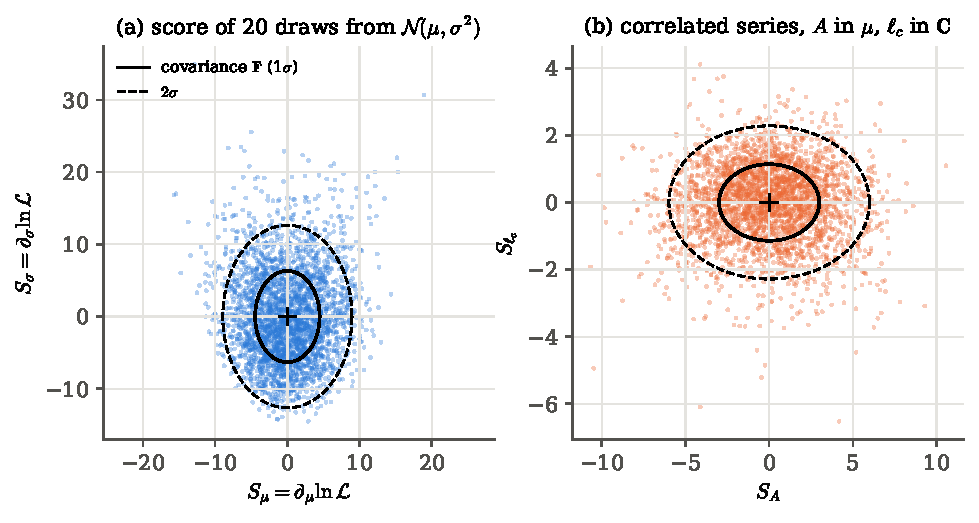
\includegraphics[width=0.98\linewidth]{figures/ch10/score_cloud.pdf}
\caption{The score is a random vector whose covariance is the Fisher matrix. Each point is the slope of the
log-likelihood of one simulated data set, evaluated at the true parameters; the solid and dashed ellipses
are drawn from $\Fish$ alone. Left: 20 Gaussian draws, parameters $(\mu,\sigma)$. Right: a correlated time
series in which the amplitude $A$ enters the mean and the correlation length $\ell_c$ enters the covariance
(\cref{10a:sec:gauss}).}
\label{10a:fig:score-cloud}
\end{figure}

\subsection{Example: forecasting Cowan's angular distribution}
\label{10a:sec:cowan}

Back to the two proposals. Cowan used this very density to ask a question every experimenter meets
\srcref{Cowan}{\S6.8}: \emph{how precisely can two shape parameters be pulled out of one finite sample, and
does the error bar read off a single fit agree with the scatter we would see if the experiment were
repeated many times?} The second half matters because in practice there is only one data set, and the
error bar quoted from it has to stand in for the scatter of experiments that will never be done.

\emph{His setup.} The density \eqref{10a:eq:cowan-pdf}, seen through the window $-0.95\le x\le0.95$, with true
values $\alpha=\beta=0.5$. He generated one sample of $2000$ events, found the maximum of the likelihood, and
read the errors and the correlation off the numerical Hessian of that one fit \srcref{Cowan}{(6.28)}. Then he
generated $500$ further samples of $2000$ events, fitted each, and took the standard deviations and the
correlation of the $500$ estimates \srcref{Cowan}{(6.29)}. His numbers are in the first two rows of
\cref{10a:tab:cowan}. Our question: can we predict them without generating a single event?

\emph{The log-density of one event.} With $g(x)=1+\alpha x+\beta x^2$ and the normalisation over the window
$[a,b]=[-0.95,0.95]$,
\[
  \mathcal N(\alpha,\beta)=\int_a^bg\,\dd x=(b-a)+\alpha\frac{b^2-a^2}2+\beta\frac{b^3-a^3}3,
  \qquad
  \ln f=\ln g(x)-\ln\mathcal N(\alpha,\beta).
\]
\emph{Its score.} Differentiating, $\partial_\alpha\ln f=x/g-\mathcal N_\alpha/\mathcal N$ and
$\partial_\beta\ln f=x^2/g-\mathcal N_\beta/\mathcal N$, with $\mathcal N_\alpha=(b^2-a^2)/2$ and
$\mathcal N_\beta=(b^3-a^3)/3$ the derivatives of the normalisation.
\emph{The Fisher matrix per event} is the covariance of this score, an integral over the model:
\begin{equation}
  I_{ij}=\E[\partial_i\ln f\,\partial_j\ln f]=\int_a^b\partial_i\ln f\;\partial_j\ln f\;f(x)\,\dd x,
  \label{10a:eq:cowan-fisher}
\end{equation}
which we do by numerical quadrature:
\pyfile[firstline=41,lastline=54,firstnumber=41]{code/ch10/01_cowan_two_param.py}{The Fisher matrix of one event: the covariance of the score, integrated over the model}
Lines 46--48 are the score written above; line 53 is \eqref{10a:eq:cowan-fisher}, one quadrature per matrix
element. No random number appears anywhere. It gives $I_{\alpha\alpha}=\TenACowIaa$, $I_{\alpha\beta}=\TenACowIab$ and
$I_{\beta\beta}=\TenACowIbb$. \emph{Many events.} The events are independent, so $\Fish=2000\,\bm I$, with
entries $F_{\alpha\alpha}=\TenACowFaa$, $F_{\alpha\beta}=\TenACowFab$ and $F_{\beta\beta}=\TenACowFbb$.

\emph{The forecast is the inverse.} For a symmetric $2\times2$ matrix the inverse is the swapped diagonal with
the off-diagonal negated, divided by the determinant:
\begin{equation}
  \Fish^{-1}=\frac1{\det\Fish}\begin{pmatrix}F_{\beta\beta}&-F_{\alpha\beta}\\-F_{\alpha\beta}&F_{\alpha\alpha}\end{pmatrix},
  \qquad \det\Fish=F_{\alpha\alpha}F_{\beta\beta}-F_{\alpha\beta}^2 ,
  \label{10a:eq:inv22}
\end{equation}
as multiplying it by $\Fish$ confirms. The diagonal entries are the variances and the off-diagonal entry the
covariance, so
\begin{equation*}
  \sigma_\alpha^2=\frac{F_{\beta\beta}}{\det\Fish},\qquad
  \sigma_\beta^2=\frac{F_{\alpha\alpha}}{\det\Fish},\qquad
  \rho=\frac{(\Fish^{-1})_{\alpha\beta}}{\sigma_\alpha\sigma_\beta}
      =\frac{-F_{\alpha\beta}/\det\Fish}{\sqrt{F_{\alpha\alpha}F_{\beta\beta}}/\det\Fish}
      =-\frac{F_{\alpha\beta}}{\sqrt{F_{\alpha\alpha}F_{\beta\beta}}} .
\end{equation*}
With the numbers above, $\det\Fish=\TenACowFaa\times\TenACowFbb-(\TenACowFab)^2\approx3.6\times10^4$, so
$\sigma_\alpha=\sqrt{\TenACowFbb/\det\Fish}=\TenACowSa$, $\sigma_\beta=\sqrt{\TenACowFaa/\det\Fish}=\TenACowSb$, and
$\rho=-(\TenACowFab)/\sqrt{\TenACowFaa\times\TenACowFbb}=+\TenACowRho$. A negative entry of the
Fisher matrix becomes a positive correlation: the sign flips in the inverse.

\emph{Our own repeats.} To have a second set of repeats with known code, \pyname{01_cowan_two_param.py} also
generates $\TenACowNexp$ experiments of $\TenACowNev$ events, fits each by Newton--Raphson, and records the observed
Hessian of the first one (\cref{10a:fig:cowan-scatter}).

\begin{table}[htbp]
\centering
\small
\renewcommand{\arraystretch}{1.15}
\begin{tabular}{@{}l ccc@{}}
\toprule
 & $\sigma_\alpha$ & $\sigma_\beta$ & $\rho$\\\midrule
Cowan, Hessian of one fit & 0.052 & 0.11 & 0.46\\
Cowan, scatter of $500$ fits & 0.051 & 0.111 & 0.42\\
ours, Fisher forecast (no events) & $\TenACowSa$ & $\TenACowSb$ & $\TenACowRho$\\
ours, Hessian of one fit & $\TenACowOneSa$ & $\TenACowOneSb$ & $\TenACowOneRho$\\
ours, scatter of $\TenACowNexp$ fits & $\TenACowMSa$ & $\TenACowMSb$ & $\TenACowMRho$\\
\bottomrule
\end{tabular}
\caption{Cowan's two-parameter example \srcref{Cowan}{(6.28)--(6.29)}, $2000$ events at $\alpha=\beta=0.5$. A standard
deviation estimated from $500$ fits carries a sampling error of $1/\sqrt{2\times499}\approx\pm3\%$, and a correlation
$\pm(1-\rho^2)/\sqrt{500}\approx\pm0.04$.}
\label{10a:tab:cowan}
\end{table}

\emph{Why the rows differ.} The scatter of $500$ fits is itself an estimate. The standard deviation of $N$
Gaussian numbers has a relative error of $1/\sqrt{2(N-1)}$, which is $3\%$ for $N=500$, and a correlation
coefficient has an error of about $(1-\rho^2)/\sqrt N\approx0.04$. Cowan's repeats differ from the forecast by
$2\%$, $0\%$ and $0.01$, all inside these limits; ours by about $4\%$, $3\%$ and $0.01$, about one sampling error.
The single-fit rows differ for another reason. The observed Hessian $\bm{\mathcal H}$ is the curvature of one
particular likelihood, and it fluctuates from data set to data set by a relative amount of order $1/\sqrt n$
(\cref{10a:sec:fisher-def}); the Fisher matrix is its average. That is why Cowan's single fit gives $\rho=0.46$
and ours $\TenACowOneRho$, on either side of $\TenACowRho$, while their errors stay within a few per cent of the
forecast. For $2000$ events the fluctuation is small, so his first row and his second row are two estimates of
the same thing, and the Fisher matrix is the number both scatter around.

The positive correlation also has a plain reason. Over the
window the two shapes $x$ and $x^2$ both rise towards $x=+0.95$, and since the density must stay normalised,
an upward fluctuation in the number of events at large positive $x$ can be absorbed partly by $\alpha$ and
partly by $\beta$, so the two estimates tend to move together.

The answer to the proposal question is now one line. Errors scale as $1/\sqrt n$, so $500$ events in the same
window would give $\sigma_\beta=\TenACowSb\times\sqrt{2000/500}\approx0.22$. A wider window changes $\bm I$
itself, and the same quadrature, with $a$ and $b$ changed, tells us by how much.

The lesson: the forecast and the repeated experiment agree to within the error of the repeats, so the
expensive part of Cowan's study, the $500$ simulated experiments, could have been replaced by one integral
per matrix element; what a single fit adds is a curvature that wobbles about that integral.

\begin{figure}[htbp]
\centering
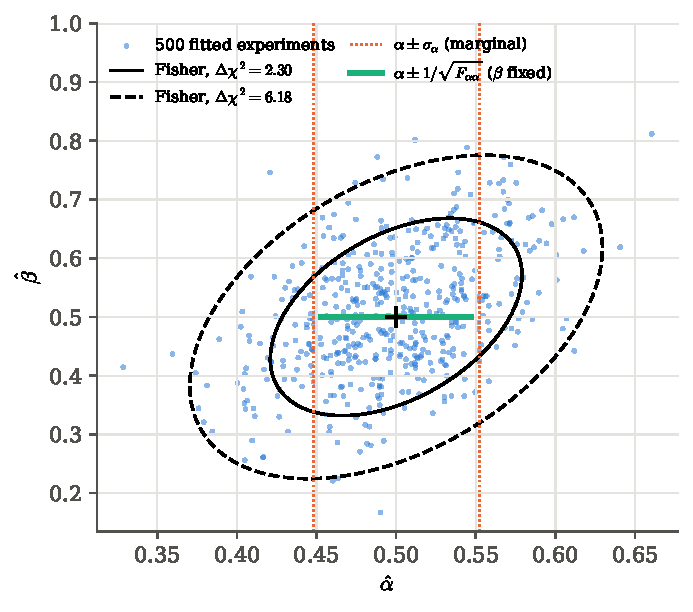
\includegraphics[width=0.62\linewidth]{figures/ch10/cowan_scatter.pdf}
\caption{Cowan's experiment repeated: each point is the maximum-likelihood fit of one simulated experiment
of $2000$ events. The ellipses come from the Fisher matrix alone, computed before any event was generated:
the solid one should contain $68.3\%$ of the points and the dashed one $95.4\%$ (\cref{10a:sec:ellipses}).
The dotted vertical lines are $\alpha\pm\sigma_\alpha$; the green bar is the shorter error on $\alpha$ that
we would quote if $\beta$ were known (\cref{10a:sec:marginal}).}
\label{10a:fig:cowan-scatter}
\end{figure}

\begin{keyidea}[The Fisher matrix]
$F_{ij}=-\E[\partial_i\partial_j\ln\Like]=\E[S_iS_j]$, evaluated at the fiducial parameters, is the average
curvature of the log-likelihood and the covariance of the score. It needs a model of the experiment, not
data. Its inverse is the forecast covariance of the parameters, and independent data sets add their Fisher
matrices.
\end{keyidea}
\section{Nobody beats the inverse Fisher matrix: the Cram\'er--Rao bound}
\label{10a:sec:cr}

The forecast of \cref{10a:sec:cowan} was built from the width of the likelihood. But the analysis team may not
use the likelihood at all. They might fit moments of the distribution, or train a network to map histograms
to parameters, or use some estimator nobody has thought of yet. Is $\Fish^{-1}$ a property of one
particular method, maximum likelihood, or is it a limit on every method? If it is a limit, a forecast is
much more than a guess: it is the best any analysis of that experiment can ever do.

For one parameter the answer was the Cram\'er--Rao inequality of \cref{3b:sec:cramer-rao}: every unbiased
estimator has $\Var\hat\theta\ge1/I_n(\theta)$ \srcref{CasellaBerger}{Thm.~7.3.9}, \srcref{Cowan}{(6.16)}. With
several parameters, a new question appears that the one-parameter bound cannot answer.

\paragraph{The question in words.} Can any unbiased method of turning the data into estimates
$\bm T(\data)=(T_1,\dots,T_m)$ have, \emph{in some direction of parameter space}, a smaller scatter than
$\Fish^{-1}$ predicts? And when we quote the error on one parameter, is the limit $1/\sqrt{F_{ii}}$, which
looks only at the $i$-th diagonal element, or $\sqrt{(\Fish^{-1})_{ii}}$, which involves the whole matrix?

\subsection{The bound, from one covariance matrix}
\label{10a:sec:cr-derive}

Let $\bm T$ be unbiased, $\E_{\params}\bm T=\params$ for every $\params$, with covariance matrix
$\bm V=\Cov\bm T$, and let $\bm S$ be the score of the whole data set. The proof needs one fact about how
$\bm T$ and $\bm S$ are related, and one fact about covariance matrices.

\emph{How the estimator and the score are correlated.} For each pair $a,j$,
\begin{align}
  \Cov(T_a,S_j)
  &\eqby{1}\E[T_a\,S_j]
  \eqby{2}\int T_a(\data)\,\frac{\partial_jp(\data\given\params)}{p(\data\given\params)}\,p(\data\given\params)\,\dd\data
  \eqby{3}\partial_j\int T_a(\data)\,p(\data\given\params)\,\dd\data
  \eqby{4}\partial_j\theta_a=\delta_{aj}.
  \label{10a:eq:cov-TS}
\end{align}
\begin{explain}
  \item $\Cov(T_a,S_j)=\E[T_aS_j]-\E T_a\,\E S_j$, and $\E S_j=0$ by \eqref{10a:eq:score-mean}.
  \item Write the expectation as an integral; $S_j=\partial_jp/p$.
  \item Cancel $p$ and take the derivative out of the integral. $T_a$ depends on the data only, not on
        $\params$; the exchange is the same regularity condition as before.
  \item The integral is $\E T_a$, which equals $\theta_a$ because the estimator is unbiased.
\end{explain}
So an unbiased estimator must be correlated with the score in a fixed way: $\Cov(\bm T,\bm S)=\Id$. This
is the whole content of unbiasedness for the proof. If $\bm T$ did not respond to the data along the
directions in which the data respond to $\params$, it could not follow $\params$ on average.

\emph{Covariance matrices are positive semidefinite.} Stack the $2m$ random numbers $(\bm T,\bm S)$ into one
vector. Its covariance matrix is
\begin{equation}
  \bm M=\begin{pmatrix}\bm V&\Id\\ \Id&\Fish\end{pmatrix},
  \qquad
  (\bm u\T,\bm w\T)\,\bm M\begin{pmatrix}\bm u\\ \bm w\end{pmatrix}=\Var(\bm u\T\bm T+\bm w\T\bm S)\ge0
  \quad\text{for all }\bm u,\bm w,
  \label{10a:eq:joint-cov}
\end{equation}
where the off-diagonal blocks are \eqref{10a:eq:cov-TS} and the lower block is \eqref{10a:eq:two-faces}.

\emph{The bound.} Pick any direction $\bm a$ in parameter space and set $\bm u=\bm a$, $\bm w=-\Fish^{-1}\bm a$:
\begin{align}
  0&\relby{1}{\le}\Var\bigl(\bm a\T\bm T-\bm a\T\Fish^{-1}\bm S\bigr)
  \eqby{2}\bm a\T\bm V\bm a-2\,\bm a\T\Fish^{-1}\bm a+\bm a\T\Fish^{-1}\Fish\Fish^{-1}\bm a
  \eqby{3}\bm a\T\bigl(\bm V-\Fish^{-1}\bigr)\bm a .
  \label{10a:eq:cr-multi}
\end{align}
\begin{explain}
  \item \eqref{10a:eq:joint-cov} with this choice of $\bm u,\bm w$.
  \item Expand the quadratic form block by block: $\bm u\T\bm V\bm u+2\bm u\T\Id\,\bm w+\bm w\T\Fish\bm w$,
        using $\Fish^{-1}$ symmetric.
  \item $\Fish^{-1}\Fish=\Id$; collect.
\end{explain}
\emph{Why that choice of $\bm w$?} One parameter shows it. Then $T$ and $S$ are two random numbers with
$\Cov(T,S)=1$ by \eqref{10a:eq:cov-TS} and $\Var S=F$. Ask for the multiple $cS$ of the score that comes closest
to $T$, in the sense of the smallest variance of the difference:
\begin{align*}
  \Var(T-cS)
  &\eqby{1}\Var T-2c\,\Cov(T,S)+c^2\Var S
   \eqby{2}\Var T-2c+c^2F ,
  \\
  \frac{\dd}{\dd c}\Var(T-cS)=-2+2cF=0
  &\eqby{3}c=\frac1F ,
  \qquad
  \Var\Bigl(T-\frac SF\Bigr)\eqby{4}\Var T-\frac1F .
\end{align*}
\begin{explain}
  \item The variance of a difference.
  \item Insert $\Cov(T,S)=1$ and $\Var S=F$.
  \item The best coefficient is covariance over variance, as in a least-squares regression of $T$ on $S$.
  \item Put $c=1/F$ back into the first line: $\Var T-2/F+1/F$.
\end{explain}
The residual $T-S/F$ is uncorrelated with the score, $\Cov(T-S/F,S)=1-F/F=0$: it is the part of $T$ the score
cannot predict. Its variance cannot be negative, so $\Var T\ge1/F$. The variance of any unbiased $T$ splits
into a part $1/F$ that is forced by its correlation with the score and a leftover that a good estimator makes
small. With many parameters the same regression of $\bm a\T\bm T$ on the score vector has coefficient vector
$\Fish^{-1}\bm a$ (covariance $\bm a\T\Id$ times the inverse of the variance matrix $\Fish$), which is exactly the
$\bm w=-\Fish^{-1}\bm a$ chosen above, and \eqref{10a:eq:cr-multi} is the matrix version of the last line.
Since $\bm a$ was arbitrary,
\begin{equation}
  \boxed{\Cov\bm T-\Fish^{-1}\succeq0:\qquad
  \Var(\bm a\T\bm T)\ge\bm a\T\Fish^{-1}\bm a\ \text{for every }\bm a,\qquad
  \Var T_i\ge(\Fish^{-1})_{ii},}
  \label{10a:eq:cr-box}
\end{equation}
where $\succeq0$ means positive semidefinite.
The last form is the choice $\bm a=\bm e_i$, the $i$-th unit vector \srcref{Cowan}{(6.19)}, \cite{TTH1997}.
Positive semidefinite ordering has a picture: the ellipse of $\Cov\bm T$ contains the ellipse of $\Fish^{-1}$,
because the half-width of an ellipse $\{\bm x:\bm x\T\bm V^{-1}\bm x\le1\}$ measured along a unit direction
$\bm a$ is $\sqrt{\bm a\T\bm V\bm a}$ (\cref{10a:fig:cr-nest}).

\begin{figure}[htbp]
\centering
\begin{tikzpicture}[scale=1.15]
  \draw[->,faint] (-2.6,0) -- (2.7,0) node[right,black,lbl] {$\theta_1$};
  \draw[->,faint] (0,-1.9) -- (0,2.0) node[above,black,lbl] {$\theta_2$};
  \draw[fibreorange,very thick,rotate=28] (0,0) ellipse (2.25 and 1.15);
  \draw[formblue,very thick,rotate=33] (0,0) ellipse (1.65 and 0.62);
  \draw[tangentgreen!80!black,thick,->] (0,0) -- (-0.55,1.6);
  \node[lbl,tangentgreen!70!black,anchor=east] at (-0.6,1.65) {direction $\bm a$};
  \node[lbl,fibreorange,anchor=west] at (1.75,1.65) {$\Cov\bm T$, any unbiased method};
  \node[lbl,formblue,anchor=west] at (1.2,-0.55) {$\Fish^{-1}$};
\end{tikzpicture}
\caption{The Cram\'er--Rao bound as a picture. For every direction $\bm a$, the spread of an unbiased
estimator along $\bm a$ is at least $\sqrt{\bm a\T\Fish^{-1}\bm a}$, so the error ellipse of any method (orange)
encloses the ellipse of the inverse Fisher matrix (blue). Maximum likelihood with informative data shrinks
its ellipse onto the blue one.}
\label{10a:fig:cr-nest}
\end{figure}

\subsection{Marginalised or conditional: the second half of the answer}
\label{10a:sec:cr-diag}

The bound on $T_i$ is $(\Fish^{-1})_{ii}$, the $ii$ element of the \emph{inverse}. How does it compare with
$1/F_{ii}$, the inverse of the $ii$ element? Two tools are needed. \emph{Picking out an element.} Write $\bm e_i$
for the unit vector with $1$ in place $i$ and $0$ elsewhere; then $\bm M\bm e_i$ is the $i$-th column of a matrix
$\bm M$ and $\bm e_i\T\bm M\bm e_i=M_{ii}$. \emph{A square root of $\Fish$.} A symmetric matrix can be written as
$\Fish=\bm V\diag(\lambda_1,\dots,\lambda_m)\bm V\T$, with the orthonormal eigenvectors as the columns of $\bm V$
($\bm V\T\bm V=\Id$) and the eigenvalues $\lambda_a$ on the diagonal; for a positive definite $\Fish$ all
$\lambda_a>0$. Then $\Fish^{1/2}\equiv\bm V\diag(\sqrt{\lambda_a})\bm V\T$ is symmetric and squares to $\Fish$, because the
inner $\bm V\T\bm V$ is $\Id$; likewise $\Fish^{-1/2}\equiv\bm V\diag(1/\sqrt{\lambda_a})\bm V\T$, and
$\Fish^{1/2}\Fish^{-1/2}=\Id$. Then
\begin{align}
  1\eqby{1}\bigl(\bm e_i\T\bm e_i\bigr)^2
  \eqby{2}\bigl[(\Fish^{1/2}\bm e_i)\T(\Fish^{-1/2}\bm e_i)\bigr]^2
  \relby{3}{\le}\bigl(\bm e_i\T\Fish\bm e_i\bigr)\bigl(\bm e_i\T\Fish^{-1}\bm e_i\bigr)
  =F_{ii}\,(\Fish^{-1})_{ii},
  \label{10a:eq:diag-ineq}
\end{align}
\begin{explain}
  \item A unit vector has length one.
  \item Insert $\Fish^{1/2}\Fish^{-1/2}=\Id$ between the two factors; both matrices are symmetric.
  \item Cauchy--Schwarz for ordinary vectors, $(\bm x\T\bm y)^2\le(\bm x\T\bm x)(\bm y\T\bm y)$.
\end{explain}
so $(\Fish^{-1})_{ii}\ge1/F_{ii}$.

\emph{When are the two equal?} Cauchy--Schwarz is an equality only when the two vectors are parallel,
$\Fish^{1/2}\bm e_i=c\,\Fish^{-1/2}\bm e_i$ for some number $c$. Multiplying both sides by $\Fish^{1/2}$ turns this into
$\Fish\bm e_i=c\,\bm e_i$: the $i$-th column of $\Fish$ has a single nonzero entry, on the diagonal. So $F_{ji}=0$
for every $j\neq i$, and parameter $i$ shares no information with any other. Then $\Fish^{-1}\bm e_i=\bm e_i/c$ as
well, and $(\Fish^{-1})_{ii}=1/F_{ii}$. In every other case the inverse of the matrix gives the larger number.
A small example gives the size: for $F_{11}=2$, $F_{22}=1$, $F_{12}=1$ the determinant is $1$ and
$(\Fish^{-1})_{11}=F_{22}/\det\Fish=1$ by \eqref{10a:eq:inv22}, so $F_{11}(\Fish^{-1})_{11}=2$: the error on $\theta_1$ is
$\sqrt2$ times larger when $\theta_2$ must be estimated too. This is the content of Tegmark, Taylor and Heavens' statement of the bound \cite{TTH1997}: $1/\sqrt{F_{ii}}$
is the smallest error on $\theta_i$ \emph{if all the other parameters are known}; if they are estimated from
the same data, the smallest error rises to $\sqrt{(\Fish^{-1})_{ii}}$. We come back to this distinction, the
single most common error in quoting forecasts, in \cref{10a:sec:marginal}. In the angular-distribution experiment of \cref{10a:sec:cowan} (Cowan's two-parameter example) the two
numbers for $\alpha$ are $1/\sqrt{F_{\alpha\alpha}}=\TenACowCondA$ and $\sqrt{(\Fish^{-1})_{\alpha\alpha}}=\TenACowSa$
(\cref{10a:fig:cowan-scatter}, green bar against dotted lines).

\subsection{When the bound is reached, and what it means}
\label{10a:sec:cr-reach}

A bound is only useful if someone reaches it. Vallisneri lists three readings of $\Fish^{-1}$ that are often
confused \cite{Vallisneri2008}: (i) the Cram\'er--Rao bound on any unbiased estimator, a statement about the
scatter over imagined repetitions of the experiment; (ii) the covariance of the maximum-likelihood
estimator, which reaches the bound when the model is linear in $\params$ over the region where the errors
live; (iii) the covariance of the Bayesian posterior from \emph{one} experiment, with a flat prior, in the
same limit. The first is always true; the second and third need a condition, and the examples show what the
condition means.

\paragraph{When is the bound an equality, and what if the estimator is biased?} Equality in \eqref{10a:eq:cr-multi}
needs $\Var(\bm a\T\bm T-\bm a\T\Fish^{-1}\bm S)=0$ for every $\bm a$. A random variable with zero variance is a
constant, and since both $\bm T$ and $\bm S$ have the right means ($\bm\theta$ and $\bm0$) the constant is $\bm\theta$ itself:
\[
  \bm T(\data)=\params+\Fish^{-1}\bm S(\data)\quad\text{for all data.}
\]
So an estimator reaches the bound exactly when the score is a linear function of the estimator. This is the case
for the linear-Gaussian model below, where the score is $\bm A\T\Cmat^{-1}(\data-\bm A\params)$, and it holds only
approximately in the other models of this chapter. The ratio
$e=\bigl[(\Fish^{-1})_{ii}\bigr]\big/\Var T_i\le1$ is the \newterm{efficiency} of the estimator \srcref{Cowan}{\S6.6}:
how much of the available information it uses.

\emph{A biased estimator.} Suppose instead $\E\bm T=\params+\bm b(\params)$, with a bias $\bm b$ that may depend on the
parameters, and write $B_{aj}=\partial_jb_a$ for its derivatives. Only the last step of \eqref{10a:eq:cov-TS}
changes: the integral is now $\E T_a=\theta_a+b_a$, so
\[
  \Cov(T_a,S_j)=\partial_j(\theta_a+b_a)=\delta_{aj}+B_{aj},
  \qquad\text{that is}\qquad \Cov(\bm T,\bm S)=\Id+\bm B ,
\]
and the off-diagonal blocks of \eqref{10a:eq:joint-cov} become $\Id+\bm B$ and $(\Id+\bm B)\T$. Repeat the
regression with the new covariance: $\bm u=\bm a$ and $\bm w=-\Fish^{-1}(\Id+\bm B)\T\bm a$. Then
\begin{align*}
  0&\relby{1}{\le}\bm a\T\bm V\bm a+2\,\bm a\T(\Id+\bm B)\bm w+\bm w\T\Fish\bm w
  \\
  &\eqby{2}\bm a\T\bm V\bm a-2\,\bm a\T(\Id+\bm B)\Fish^{-1}(\Id+\bm B)\T\bm a
    +\bm a\T(\Id+\bm B)\Fish^{-1}\Fish\Fish^{-1}(\Id+\bm B)\T\bm a
  \\
  &\eqby{3}\bm a\T\bigl[\bm V-(\Id+\bm B)\Fish^{-1}(\Id+\bm B)\T\bigr]\bm a .
\end{align*}
\begin{explain}
  \item The quadratic form of the joint covariance, expanded block by block, is a variance and so not negative.
  \item Insert $\bm w$; its transpose is $-\bm a\T(\Id+\bm B)\Fish^{-1}$, since $\Fish^{-1}$ is symmetric.
  \item $\Fish^{-1}\Fish=\Id$, so the last term is $\bm a\T(\Id+\bm B)\Fish^{-1}(\Id+\bm B)\T\bm a$, and the middle term is
        $-2$ times the same number; together they leave minus it once.
\end{explain}
Since $\bm a$ is arbitrary,
\begin{equation}
  \Cov\bm T\succeq(\Id+\bm B)\,\Fish^{-1}(\Id+\bm B)\T ,
  \label{10a:eq:cr-bias}
\end{equation}
which is the information inequality of \srcref{Cowan}{(6.16)} for several parameters. With $\bm B=\bm0$ it is
\eqref{10a:eq:cr-box} again.

\emph{A bias can buy a smaller variance.} Take $n$ draws from $\Normal(\theta,\sigma^2)$ with known $\sigma$, so
$F=n/\sigma^2$, and shrink the sample mean towards zero: $T=c\,\bar x$ with $0<c<1$. Its mean is $c\theta$, so the bias
is $b=-(1-c)\theta$ and $B=\dd b/\dd\theta=-(1-c)$, giving $1+B=c$. The bound \eqref{10a:eq:cr-bias} reads
$\Var T\ge c^2/F=c^2\sigma^2/n$, and indeed $\Var T=c^2\Var\bar x=c^2\sigma^2/n$: the shrunk estimator sits on its
bound, which is below the unbiased bound $1/F=\sigma^2/n$ by the factor $c^2$. A bias whose derivative is
negative pulls estimates together, and the variance drops below $\Fish^{-1}$; the price is that $T$ is off
by $(1-c)\theta$ on average. This is the loophole of the last example below.

\paragraph{Example: a linear model reaches the bound exactly.} Let the data be $\data=\bm A\params+\bm n$
with a known $N\times m$ matrix $\bm A$ (each column a template, for example the columns $1$ and $x$ of a
straight-line fit) and Gaussian noise $\bm n\sim\Normal(\bm0,\Cmat)$ with known $\Cmat$. Then
$\ln\Like=-\tfrac12(\data-\bm A\params)\T\Cmat^{-1}(\data-\bm A\params)+\text{const}$ and
\begin{align*}
  -\partial_i\partial_j\ln\Like
  &\eqby{1}(\bm A\T\Cmat^{-1}\bm A)_{ij}\equiv F_{ij},
  \\
  \hat\params&\eqby{2}(\bm A\T\Cmat^{-1}\bm A)^{-1}\bm A\T\Cmat^{-1}\data=\Fish^{-1}\bm A\T\Cmat^{-1}\data,
  \\
  \Cov\hat\params
  &\eqby{3}\Fish^{-1}\bm A\T\Cmat^{-1}\,\Cov(\data)\,\Cmat^{-1}\bm A\,\Fish^{-1}
  \eqby{4}\Fish^{-1}\bigl(\bm A\T\Cmat^{-1}\bm A\bigr)\Fish^{-1}
  =\Fish^{-1}.
\end{align*}
\begin{explain}
  \item Differentiate the quadratic form twice: the second derivative is constant, the same for every data
        set, so no average is needed.
  \item Set the gradient $\bm A\T\Cmat^{-1}(\data-\bm A\params)$ to zero: the normal equations of
        \cref{ch:03}.
  \item $\hat\params$ is a linear map $\bm B\data$ of the data, so $\Cov\hat\params=\bm B\Cov(\data)\bm B\T$;
        the term $\bm A\params$ in $\data$ is not random.
  \item $\Cov(\data)=\Cmat$, and $\Cmat^{-1}\Cmat\Cmat^{-1}=\Cmat^{-1}$.
\end{explain}
The bound is reached exactly, at any number of data points. The log-likelihood is an exact parabola in
$\params$, its curvature is the same for every data set, and all three readings of $\Fish^{-1}$ coincide.
Every other situation is this one only approximately: a nonlinear model looks linear when the errors are
small compared with the scale on which the model bends, which is what ``informative data'' or ``high
signal-to-noise'' means.

\paragraph{Example: how fast does Cowan's experiment reach the bound?} The angular distribution is not linear in
$(\alpha,\beta)$, because the parameters also sit in the denominator of $\ln g$. \pyname{01_cowan_two_param.py}
repeats the experiment $\TenACowNrep$ times at each of several event numbers $n$ and compares the variance of
the fitted $\hat\alpha$ and $\hat\beta$ with the bound $(\Fish^{-1})_{ii}=(\bm I^{-1})_{ii}/n$
(\cref{10a:fig:cowan-bound}). At $n=2000$ the ratios are $\TenACowRatioTwoK$ and $\TenACowRatioTwoKB$, one within
the simulation error of about $\pm\TenACowRatioErr$. At $n=50$ they are $\TenACowRatioFifty$ and
$\TenACowRatioFiftyB$, and in $\TenACowRunFifty\%$ of the experiments the fit does not converge at all: the
likelihood keeps increasing as $\beta\to\infty$, because a handful of events all at large $\abs x$ look like a
pure $x^2$ shape. With so little information the log-likelihood is far from a parabola over the range where
the estimates scatter, and a Fisher forecast for $50$ events would be too optimistic by a quarter in
$\sigma_\alpha$.

\begin{figure}[htbp]
\centering
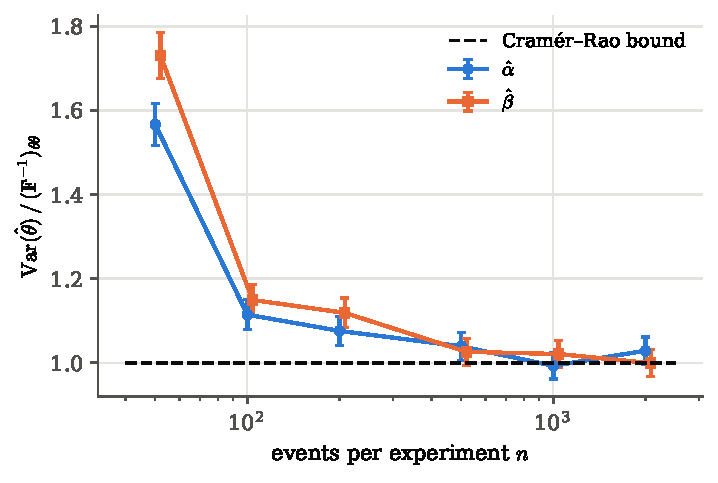
\includegraphics[width=0.66\linewidth]{figures/ch10/cowan_bound.pdf}
\caption{The variance of the maximum-likelihood estimates in Cowan's experiment divided by the Cram\'er--Rao
bound, against the number of events. Below a few hundred events the fits scatter more than the bound; from
about $500$ events on, maximum likelihood reaches it. Error bars are the Monte Carlo uncertainty of a
variance estimated from $2000$ experiments.}
\label{10a:fig:cowan-bound}
\end{figure}

\paragraph{Example: the bound is for unbiased estimators.} Two loopholes are worth naming. First, a biased
estimator can beat $\Fish^{-1}$. The posterior mean with an informative prior is one: it is pulled towards
the prior, and its scatter is smaller, which is fair because the prior is extra information. In the Fisher
language the prior simply adds its own matrix (\cref{10a:sec:priors}). Second, the bound needs the regularity
condition: for $\mathrm{Uniform}(0,\theta)$ the maximum of the sample has a variance falling like $1/n^2$
(\cref{3b:sec:cramer-rao}), because a sharp edge in the data is not covered by the derivation. In the other
direction, the bound does not promise that a good estimator exists at small $n$. Take the variance of a
Gaussian with unknown mean, now with $(\mu,\sigma^2)$ as parameters instead of $(\mu,\sigma)$. \emph{The bound.} The
Jacobian rule \eqref{10a:eq:jacobian} converts the Fisher entry for $\sigma$ found in \cref{10a:sec:two-faces} into
one for $\sigma^2$: with $\sigma=\sqrt{\sigma^2}$, $\dd\sigma/\dd\sigma^2=1/(2\sigma)$, so
\[
  F_{\sigma^2\sigma^2}=\Bigl(\frac{\dd\sigma}{\dd\sigma^2}\Bigr)^2F_{\sigma\sigma}=\frac1{4\sigma^2}\,\frac{2n}{\sigma^2}=\frac n{2\sigma^4},
\]
while $F_{\mu\mu}=n/\sigma^2$ and the off-diagonal entry stay as they were, zero. The matrix is diagonal, so the bound
on any unbiased estimator of $\sigma^2$ is the inverse of this one entry, $2\sigma^4/n$. \emph{The best unbiased
estimator.} The sample variance $S^2$ has $(n-1)S^2/\sigma^2\sim\chi^2_{n-1}$, and a $\chi^2_k$ variable has variance
$2k$, so $\Var S^2=\sigma^4\cdot2(n-1)/(n-1)^2=2\sigma^4/(n-1)$, as in \eqref{3a:eq:var-s2-gauss}. It exceeds the
bound by the factor $n/(n-1)$, and no unbiased estimator does better \srcref{CasellaBerger}{Ex.~7.3.14}: the bound is
approached only as $n$ grows.

\begin{keyidea}[Cram\'er--Rao for many parameters]
For any unbiased estimator, $\Cov\bm T-\Fish^{-1}$ is positive semidefinite: no direction of parameter space
can be measured better than $\Fish^{-1}$ allows. The error on one parameter is at least
$\sqrt{(\Fish^{-1})_{ii}}\ge1/\sqrt{F_{ii}}$, the second value applying only when all other parameters are
known. Maximum likelihood reaches the bound exactly for linear-Gaussian models and approximately whenever
the data are informative enough that the log-likelihood is a parabola over the scatter of the estimates.
\end{keyidea}
\section{Gaussian data: the Fisher matrix in closed form}
\label{10a:sec:gauss}

Most data in physics reach the analysis as a Gaussian vector, or are compressed into one. The pixels of a CMB
map, its harmonic coefficients $\alm$, a binned power spectrum, the Fourier amplitudes of a detector's
strain, the points of a fitted line: each is either Gaussian by nature (a Gaussian random field, thermal
detector noise) or Gaussian to a good approximation by the central limit theorem (a bin average of many
modes, \cref{ch:02}). The parameters reach such data in two different ways. Either they move the
\emph{mean}: a peak position, a template amplitude, the shape of a gravitational waveform. Or they change the
\emph{covariance}: the CMB temperature has zero mean at every point, and every cosmological parameter acts
only through the variance $\Cell$ of the $\alm$. A forecast formula for Gaussian data must handle both, and
it turns out to be one line.

\paragraph{The question.} If the data vector $\data$ (length $N$) is Gaussian with a mean $\bm\mu(\params)$ and a
covariance $\Cmat(\params)$ that we can compute for any parameters, what is the Fisher matrix, written with
nothing but $\bm\mu$, $\Cmat$ and their derivatives?

\paragraph{The inputs.} One physical input: the data are Gaussian, with mean and covariance known as functions of
the parameters (all the physics of the experiment, signal and noise, sits in these two functions). Two
mathematical inputs: $\bm\mu$ and $\Cmat$ are differentiable in $\params$, and $\Cmat$ is positive definite,
hence invertible. Everything else is derived. With $\bm r=\data-\bm\mu$ the residual,
\begin{equation}
  -2\ln\Like(\params)=\ln\det\Cmat+\bm r\T\Cmat^{-1}\bm r+N\ln2\pi
  \label{10a:eq:gauss-like}
\end{equation}
\srcref{HobsonBMC}{(5.16)}, \cite{TTH1997}, eq.~(7). It is the likelihood in the sense of \cref{ch:03}: the data are the model mean plus noise, $\data=\bm\mu(\params)+\bm n$, and for a given $\params$ the likelihood asks how plausible the particular noise realisation $\bm r=\data-\bm\mu(\params)$ is that would turn the model into the data we have. The second term is the familiar $\chi^2$ of \cref{ch:03};
the first is what is left of the normalisation $(2\pi)^{-N/2}(\det\Cmat)^{-1/2}$, and it matters as soon as
$\Cmat$ depends on the parameters. We write $\bm\mu_{,i}=\partial_i\bm\mu$, $\Cmat_{,i}=\partial_i\Cmat$, and so on.

\subsection{Three tools}
\label{10a:sec:gauss-tools}

\emph{The derivative of an inverse.} Differentiate $\Cmat\Cmat^{-1}=\Id$: $\Cmat_{,i}\Cmat^{-1}+\Cmat\,\partial_i(\Cmat^{-1})=0$,
so
\begin{equation}
  \partial_i(\Cmat^{-1})=-\Cmat^{-1}\Cmat_{,i}\Cmat^{-1}.
  \label{10a:eq:dinv}
\end{equation}
It is the matrix version of $(1/c)'=-c'/c^2$; the order matters because matrices do not commute.

\emph{The derivative of a log-determinant.} For a small change $\delta\Cmat$,
\begin{align}
  \ln\det(\Cmat+\delta\Cmat)
  &\eqby{1}\ln\det\Cmat+\ln\det(\Id+\Cmat^{-1}\delta\Cmat)
  \eqby{2}\ln\det\Cmat+\ln\prod_a(1+\epsilon_a)
  \nonumber\\
  &\eqby{3}\ln\det\Cmat+\Tr(\Cmat^{-1}\delta\Cmat)+O(\delta^2),
  \label{10a:eq:dlogdet}
\end{align}
\begin{explain}
  \item $\Cmat+\delta\Cmat=\Cmat(\Id+\Cmat^{-1}\delta\Cmat)$, and the determinant of a product is the product of
        determinants.
  \item $\epsilon_a$ are the eigenvalues of the small matrix $\Cmat^{-1}\delta\Cmat$; a determinant is the product
        of the eigenvalues, and $\Id+\bm\epsilon$ has eigenvalues $1+\epsilon_a$.
  \item $\ln(1+\epsilon_a)=\epsilon_a+O(\epsilon^2)$, and the sum of the eigenvalues is the trace.
\end{explain}
Hence $\partial_i\ln\det\Cmat=\Tr(\Cmat^{-1}\Cmat_{,i})$, the matrix version of $(\ln c)'=c'/c$.

\emph{The average of a quadratic form.} For any fixed matrix $\bm B$ and a residual with $\E\bm r=\bm0$,
$\E\bm r\bm r\T=\Cmat$:
\begin{equation}
  \E[\bm r\T\bm B\bm r]=\E\Tr(\bm B\bm r\bm r\T)=\Tr(\bm B\,\E[\bm r\bm r\T])=\Tr(\bm B\Cmat),
  \label{10a:eq:quadform}
\end{equation}
because a number is its own trace, the trace is cyclic, and both trace and expectation are linear.
Terms linear in $\bm r$ average to zero, and terms with three factors of $\bm r$ never appear below.

\subsection{The derivation}
\label{10a:sec:gauss-derive}

\emph{The score.} Differentiate \eqref{10a:eq:gauss-like} once. The residual depends on $\params$ through the mean,
$\partial_i\bm r=-\bm\mu_{,i}$, so
\begin{align}
  \partial_i(-2\ln\Like)
  &\eqby{1}\Tr(\Cmat^{-1}\Cmat_{,i})-2\bm\mu_{,i}\T\Cmat^{-1}\bm r-\bm r\T\Cmat^{-1}\Cmat_{,i}\Cmat^{-1}\bm r .
  \label{10a:eq:gauss-score}
\end{align}
\begin{explain}
  \item The first term is \eqref{10a:eq:dlogdet}. In the quadratic form, differentiating either of the two
        $\bm r$ gives $-\bm\mu_{,i}\T\Cmat^{-1}\bm r$ (the two are equal because $\Cmat^{-1}$ is symmetric), and
        differentiating $\Cmat^{-1}$ uses \eqref{10a:eq:dinv}.
\end{explain}
Its average is $\Tr(\Cmat^{-1}\Cmat_{,i})-0-\Tr(\Cmat^{-1}\Cmat_{,i}\Cmat^{-1}\Cmat)=0$ by
\eqref{10a:eq:quadform}: the score has mean zero, as it must.

\emph{The second derivative.} Differentiate each of the three terms of \eqref{10a:eq:gauss-score} with respect
to $\theta_j$, and average at once, dropping every term linear in $\bm r$:
\begin{align}
  \E\,\partial_j\Tr(\Cmat^{-1}\Cmat_{,i})
  &\eqby{1}-\Tr(\Cmat^{-1}\Cmat_{,j}\Cmat^{-1}\Cmat_{,i})+\Tr(\Cmat^{-1}\Cmat_{,ij}),
  \nonumber\\
  \E\,\partial_j\bigl(-2\bm\mu_{,i}\T\Cmat^{-1}\bm r\bigr)
  &\eqby{2}2\,\bm\mu_{,i}\T\Cmat^{-1}\bm\mu_{,j},
  \nonumber\\
  \E\,\partial_j\bigl(-\bm r\T\Cmat^{-1}\Cmat_{,i}\Cmat^{-1}\bm r\bigr)
  &\eqby{3}\E\,\bm r\T\bigl[\Cmat^{-1}\Cmat_{,j}\Cmat^{-1}\Cmat_{,i}\Cmat^{-1}-\Cmat^{-1}\Cmat_{,ij}\Cmat^{-1}
   +\Cmat^{-1}\Cmat_{,i}\Cmat^{-1}\Cmat_{,j}\Cmat^{-1}\bigr]\bm r
  \nonumber\\
  &\eqby{4}\Tr(\Cmat^{-1}\Cmat_{,j}\Cmat^{-1}\Cmat_{,i})-\Tr(\Cmat^{-1}\Cmat_{,ij})+\Tr(\Cmat^{-1}\Cmat_{,i}\Cmat^{-1}\Cmat_{,j}).
  \label{10a:eq:gauss-hess}
\end{align}
\begin{explain}
  \item Product rule on $\Cmat^{-1}\Cmat_{,i}$, with \eqref{10a:eq:dinv} for the derivative of $\Cmat^{-1}$. Nothing
        is random here.
  \item Of the three pieces of the product rule, $-2\bm\mu_{,ij}\T\Cmat^{-1}\bm r$ and
        $+2\bm\mu_{,i}\T\Cmat^{-1}\Cmat_{,j}\Cmat^{-1}\bm r$ are linear in $\bm r$ and average to zero; the third comes
        from $\partial_j\bm r=-\bm\mu_{,j}$.
  \item The terms in which $\partial_j$ hits an $\bm r$ are linear in $\bm r$ and drop out; what is left is the
        derivative of the middle matrix $\Cmat^{-1}\Cmat_{,i}\Cmat^{-1}$, using \eqref{10a:eq:dinv} on each $\Cmat^{-1}$.
  \item \eqref{10a:eq:quadform}, then $\Cmat^{-1}\Cmat=\Id$ at the end of each product.
\end{explain}
Add the three lines. The first trace of the first line cancels the first trace of the third line (they are equal by the
cyclic property), the two $\Tr(\Cmat^{-1}\Cmat_{,ij})$ cancel, and what survives is
$2\bm\mu_{,i}\T\Cmat^{-1}\bm\mu_{,j}+\Tr(\Cmat^{-1}\Cmat_{,i}\Cmat^{-1}\Cmat_{,j})$. Dividing by two,
\begin{equation}
  \boxed{F_{ij}=\bm\mu_{,i}\T\,\Cmat^{-1}\bm\mu_{,j}+\frac12\Tr\bigl[\Cmat^{-1}\Cmat_{,i}\,\Cmat^{-1}\Cmat_{,j}\bigr]}
  \label{10a:eq:gauss-fisher}
\end{equation}
which is Tegmark, Taylor and Heavens' eq.~(15), there written $\frac12\Tr[\bm A_i\bm A_j+\Cmat^{-1}\bm M_{ij}]$ with
$\bm A_i=\Cmat^{-1}\Cmat_{,i}$ and $\bm M_{ij}=\bm\mu_{,i}\bm\mu_{,j}\T+\bm\mu_{,j}\bm\mu_{,i}\T$ \cite{TTH1997},
\srcref{HobsonBMC}{(5.17)}.

Three things in \eqref{10a:eq:gauss-fisher} are worth saying in words. First, \emph{only first derivatives
appear}: the second derivatives $\bm\mu_{,ij}$ and $\Cmat_{,ij}$ cancelled. A forecast needs to know how the
model responds to each parameter, and nothing more. Second, the information splits into two independent
channels (\cref{10a:fig:channels}). The mean part is a dot product of the response vectors
$\bm\mu_{,i}$ and $\bm\mu_{,j}$ in the metric $\Cmat^{-1}$: a change of $\theta_i$ is detectable if it moves the
mean by an amount that is large compared with the noise, in the direction where the noise is small. The
covariance part measures how much a change of the parameters reshapes the scatter of the data, in units of
the scatter itself. Third, the geometric reading of Tegmark et al.: if two response vectors are nearly
parallel in that metric, the two parameters do the same thing to the data, the Fisher matrix is nearly
singular, and their errors explode together. That is a degeneracy, now seen at the level of the model.

\begin{figure}[htbp]
\centering
\begin{tikzpicture}[x=0.95cm,y=2.4cm]
  \begin{scope}
    \draw[->,faint] (-3,0) -- (3.4,0) node[right,black,lbl] {$d$};
    \draw[formblue,very thick,domain=-3:3,samples=100] plot (\x,{exp(-(\x+0.5)^2/0.8)});
    \draw[fibreorange,very thick,dashed,domain=-3:3,samples=100] plot (\x,{exp(-(\x-0.6)^2/0.8)});
    \node[lbl,align=center] at (0,1.25) {mean channel: $\theta$ moves $\bm\mu$};
    \node[lbl,anchor=north] at (0,-0.05) {$\bm\mu_{,i}\T\Cmat^{-1}\bm\mu_{,j}$};
  \end{scope}
  \begin{scope}[xshift=7.4cm]
    \draw[->,faint] (-3,0) -- (3.4,0) node[right,black,lbl] {$d$};
    \draw[formblue,very thick,domain=-3:3,samples=100] plot (\x,{exp(-(\x)^2/0.5)});
    \draw[fibreorange,very thick,dashed,domain=-3:3,samples=100] plot (\x,{0.6*exp(-(\x)^2/1.4)});
    \node[lbl,align=center] at (0,1.25) {covariance channel: $\theta$ reshapes $\Cmat$};
    \node[lbl,anchor=north] at (0,-0.05) {$\tfrac12\Tr[\Cmat^{-1}\Cmat_{,i}\Cmat^{-1}\Cmat_{,j}]$};
  \end{scope}
\end{tikzpicture}
\caption{The two ways a parameter reaches Gaussian data. Left: changing $\theta$ (solid to dashed) shifts the
distribution of the data; the information is the squared shift in units of the noise. Right: changing
$\theta$ leaves the mean at zero and widens the distribution, as cosmological parameters do to the CMB
$\alm$; the information is the squared fractional change of the variance, with a factor one half.}
\label{10a:fig:channels}
\end{figure}

For simulations it is useful to have the score itself, which is minus one half of \eqref{10a:eq:gauss-score}:
\begin{equation}
  S_i=\bm\mu_{,i}\T\Cmat^{-1}\bm r+\tfrac12\bigl(\bm r\T\Cmat^{-1}\Cmat_{,i}\Cmat^{-1}\bm r-\Tr\Cmat^{-1}\Cmat_{,i}\bigr).
  \label{10a:eq:gauss-S}
\end{equation}

\subsection{Examples}
\label{10a:sec:gauss-ex}

\paragraph{Example: a template of known shape (mean channel only).} A detector sees noise of known covariance
$\Cmat$ and possibly a signal $A\bm s$ of known shape $\bm s$ and unknown amplitude $A$. Then $\bm\mu_{,A}=\bm s$,
$\Cmat_{,A}=0$, and $F_{AA}=\bm s\T\Cmat^{-1}\bm s$, so $\sigma_A=(\bm s\T\Cmat^{-1}\bm s)^{-1/2}$. The ratio of the true
amplitude to its error is the signal-to-noise ratio of a matched filter, $\SNR=A\sqrt{\bm s\T\Cmat^{-1}\bm s}$. For
white noise $\Cmat=\sigma^2\Id$ this is $\sqrt{\sum_ks_k^2}/\sigma$ times $A$: every sample adds the square of its
signal-to-noise. Part~10b uses exactly this with $\Cmat$ replaced by the noise power spectrum of a gravitational-wave
detector.

\paragraph{Example: estimating a variance (covariance channel only).} Let $N$ numbers be drawn independently from
$\Normal(0,v)$ and let the parameter be the variance $v$. Then $\bm\mu=\bm0$, $\Cmat=v\Id$, $\Cmat^{-1}\Cmat_{,v}=\Id/v$,
and
\[
  F_{vv}=\tfrac12\Tr\bigl[(\Id/v)^2\bigr]=\frac N{2v^2},
  \qquad
  \sigma_v=v\sqrt{\frac2N}.
\]
A variance estimated from $N$ independent Gaussian numbers has a fractional error $\sqrt{2/N}$, however
precisely each number is measured. This is the origin of cosmic variance: the $2\ell+1$ coefficients $\alm$ at
one multipole are $N=2\ell+1$ such numbers with variance $\Cell$, so $\sigma(\Cell)/\Cell=\sqrt{2/(2\ell+1)}$
(\cref{ch:07}). In the parameter $\sigma=\sqrt v$ the same information reads $F_{\sigma\sigma}=(\dd v/\dd\sigma)^2F_{vv}=2N/\sigma^2$,
the value found directly in \cref{10a:sec:two-faces}; this rescaling is a first instance of the
Jacobian rule of \cref{10a:sec:reparam}.

\paragraph{Example: both channels at once.} Suppose each of $n$ points is $\Normal(\theta,\theta^2)$: a quantity whose
noise grows in proportion to its size. The mean channel gives $1/\theta^2$ per point; in the covariance channel
$\Cmat=\theta^2$, $\Cmat^{-1}\Cmat_{,\theta}=2/\theta$, and $\frac12(2/\theta)^2=2/\theta^2$. In total
$F=3n/\theta^2$: here the spread of the data carries twice as much information as their average position. With
$n=\TenBScCn$ and $\theta=\TenBScCtheta$, the variance of the score \eqref{10a:eq:gauss-S} over
$\TenBScCnsim$ simulated data sets is $\TenBScCvar$, against $3n/\theta^2=\TenBScCth$.

The same example contains a warning. A Poisson count with mean $\lambda$ is often approximated by
$\Normal(\lambda,\lambda)$. The formula then gives $1/\lambda$ from the mean and $1/2\lambda^2$ from the variance, while
the exact Poisson information is $1/\lambda$ (\cref{3b:sec:fisher-info}). The Gaussian approximation invents the
extra $1/2\lambda^2$: it pretends that the observed scatter is an independent measurement of $\lambda$, which for a
Poisson variable it is not. For large $\lambda$ the invented part is negligible; for a few counts per bin it is
not, and a forecast built that way is too optimistic.

\paragraph{Example: a correlated time series in Python.} A more realistic case separates the two channels cleanly.
Forty samples $d_k$ at times $t_k$ spread over two periods carry a signal $A\sin t_k$ on top of correlated noise
plus white noise,
\[
  \mu_k=A\sin t_k,\qquad
  C_{kl}=s^2e^{-\abs{t_k-t_l}/\ell_c}+\sigma_n^2\delta_{kl},
\]
with $A=1$, $s=0.8$, $\ell_c=1.5$ and $\sigma_n=0.5$. The amplitude $A$ is in the mean only, the correlation length
$\ell_c$ is in the covariance only, so \eqref{10a:eq:gauss-fisher} has no cross term:
$F_{AA}=\TenBScBFAA$, $F_{\ell_c\ell_c}=\TenBScBFLL$, $F_{A\ell_c}=\TenBScBFAL$. The script draws $\TenBScNsim$
series, evaluates the score \eqref{10a:eq:gauss-S} for each, and finds a covariance with diagonal
$(\TenBScBcAA,\TenBScBcLL)$ and off-diagonal $\TenBScBcAL$, equal to the formula within the simulation noise of
one to two per cent (\cref{10a:fig:score-cloud}, right).

The same script asks a design question: what if we sampled the same two periods more densely?
\Cref{10a:fig:score-gauss} gives the answer. For white noise the error on $A$ would fall as $n^{-1/2}$.
Here it falls from $\TenBScSatAten$ at $10$ samples to only $\TenBScSatA$ at $320$, because the correlated part of
the noise is common to neighbouring samples and does not average down: once the samples are much closer
than $\ell_c$, a new sample repeats the noise of its neighbour. The correlation length itself keeps improving
(from $\TenBScSatLten$ to $\TenBScSatL$), because denser sampling resolves the shape of the correlation at short
separations, which is exactly where $\ell_c$ shows. Before the data are taken, the Fisher matrix tells us
which of the two quantities a denser sampling would actually buy.

\begin{figure}[htbp]
\centering
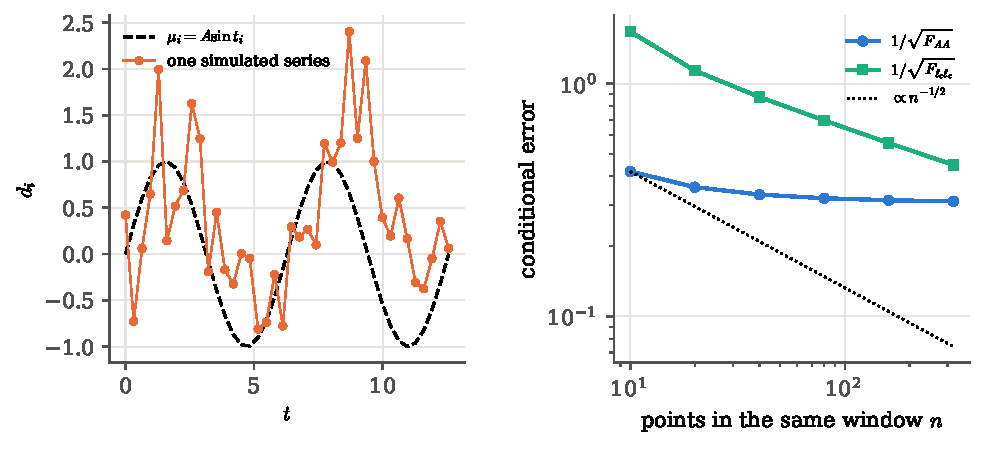
\includegraphics[width=0.98\linewidth]{figures/ch10/score_gauss.pdf}
\caption{Left: one simulated series (points) and its mean $A\sin t$ (dashed). Right: the conditional errors
$1/\sqrt{F_{ii}}$ on $A$ and $\ell_c$ when the same window is sampled with more and more points. Against the white-noise
expectation $n^{-1/2}$ (dotted), the amplitude error stalls, because correlated noise does not average down,
while the correlation length keeps improving.}
\label{10a:fig:score-gauss}
\end{figure}

\begin{keyidea}[The Fisher matrix of Gaussian data]
For $\data\sim\Normal(\bm\mu(\params),\Cmat(\params))$,
$F_{ij}=\bm\mu_{,i}\T\Cmat^{-1}\bm\mu_{,j}+\frac12\Tr[\Cmat^{-1}\Cmat_{,i}\Cmat^{-1}\Cmat_{,j}]$. Only first derivatives of
the model enter. Parameters in the mean contribute the squared shift of the mean in units of the noise;
parameters in the covariance contribute the squared fractional change of the scatter, with a factor one half.
\end{keyidea}
\section{Reading a Fisher matrix}
\label{10a:sec:reading}

A Fisher matrix for six cosmological parameters is thirty-six numbers. On its own it answers nothing; the
questions people actually ask are of a different kind. How well is $n_s$ measured if everything else is
also free? Which combination of parameters does the experiment really pin down? What if we add the
measurement of $\tau$ that another experiment already has? What is the error on $H_0$, which is not one of
the parameters we differentiated with respect to? Each question has a one-line answer in terms of $\Fish$,
and each answer comes from treating $\Fish$ as what it approximately is: the inverse covariance of a
Gaussian in parameter space, $\Like(\params)\propto\exp[-\frac12(\params-\params_0)\T\Fish(\params-\params_0)]$. This
section collects those answers and the reasons for them, then condenses them into a recipe.

\subsection{Marginal and conditional errors}
\label{10a:sec:marginal}

\paragraph{The question.} We want the error on one group of parameters $\bm a$ (say $n_s$), while the others,
$\bm b$, are also unknown. ``Also unknown'' can mean two different things. Either the other parameters are
estimated from the same data and we do not care about them: we \emph{marginalise}, averaging the Gaussian over
all their values, as in \cref{ch:01} \unpack{integrating a joint distribution over the variables we do not
want, to isolate the one we do}. Or someone tells us their values: we \emph{condition} on them, taking a
slice of the Gaussian at the known values. Which width does each give?

Split $\bm\delta=\params-\params_0$ into $(\bm\delta_a,\bm\delta_b)$ and $\Fish$ into blocks $\Fish_{aa}$, $\Fish_{ab}$,
$\Fish_{ba}=\Fish_{ab}\T$, $\Fish_{bb}$. The exponent of the Gaussian is
\begin{align}
  \bm\delta\T\Fish\bm\delta
  &\eqby{1}\bm\delta_a\T\Fish_{aa}\bm\delta_a+2\bm\delta_a\T\Fish_{ab}\bm\delta_b+\bm\delta_b\T\Fish_{bb}\bm\delta_b
  \nonumber\\
  &\eqby{2}\bigl(\bm\delta_b+\Fish_{bb}^{-1}\Fish_{ba}\bm\delta_a\bigr)\T\Fish_{bb}\bigl(\bm\delta_b+\Fish_{bb}^{-1}\Fish_{ba}\bm\delta_a\bigr)
  +\bm\delta_a\T\bigl(\Fish_{aa}-\Fish_{ab}\Fish_{bb}^{-1}\Fish_{ba}\bigr)\bm\delta_a .
  \label{10a:eq:complete-square}
\end{align}
\begin{explain}
  \item Multiply out the block form; the two cross terms are equal because $\Fish$ is symmetric.
  \item Complete the square in $\bm\delta_b$: expanding the first product gives back
        $\bm\delta_b\T\Fish_{bb}\bm\delta_b+2\bm\delta_a\T\Fish_{ab}\bm\delta_b+\bm\delta_a\T\Fish_{ab}\Fish_{bb}^{-1}\Fish_{ba}\bm\delta_a$, and the
        last piece is subtracted again in the second term.
\end{explain}
\emph{Conditioning} sets $\bm\delta_b=\bm0$ in the original exponent: what remains is $\bm\delta_a\T\Fish_{aa}\bm\delta_a$,
so the conditional covariance of $\bm a$ is $\Fish_{aa}^{-1}$. \emph{Marginalising} integrates over $\bm\delta_b$. In the
second line of \eqref{10a:eq:complete-square} the first term is a Gaussian in $\bm\delta_b$ centred on
$-\Fish_{bb}^{-1}\Fish_{ba}\bm\delta_a$ with a width that does not depend on $\bm\delta_a$, so its integral is a constant.
The marginal is a Gaussian in $\bm\delta_a$ with inverse covariance
\begin{equation}
  \widetilde{\Fish}_{aa}=\Fish_{aa}-\Fish_{ab}\Fish_{bb}^{-1}\Fish_{ba},
  \label{10a:eq:schur}
\end{equation}
the \newterm{Schur complement} of $\Fish_{bb}$ \unpack{what is left of the information on $\bm a$ after the part that
could be confused with changes of $\bm b$ is removed}. The same block also appears when we invert $\Fish$: multiplying
out shows that
\[
  \Fish\begin{pmatrix}\widetilde{\Fish}_{aa}^{-1}\\-\Fish_{bb}^{-1}\Fish_{ba}\widetilde{\Fish}_{aa}^{-1}\end{pmatrix}
  =\begin{pmatrix}(\Fish_{aa}-\Fish_{ab}\Fish_{bb}^{-1}\Fish_{ba})\widetilde{\Fish}_{aa}^{-1}\\
   (\Fish_{ba}-\Fish_{bb}\Fish_{bb}^{-1}\Fish_{ba})\widetilde{\Fish}_{aa}^{-1}\end{pmatrix}
  =\begin{pmatrix}\Id\\ \bm0\end{pmatrix},
\]
so the $aa$ block of $\Fish^{-1}$ is $\widetilde{\Fish}_{aa}^{-1}$. In words: \emph{to marginalise, invert the whole Fisher
matrix and read off the block you want} \srcref{HobsonBMC}{p.~107}, \cite{Coe2009}. The same block-inverse
formula gave conditional and marginal variances of a multivariate Gaussian in \cref{ch:02}; here the roles of
covariance and inverse covariance are exchanged.

\begin{workdef}[marginalised and conditional errors]
The \newterm{marginalised error} on $\theta_i$ is $\sigma_i=\sqrt{(\Fish^{-1})_{ii}}$, the error when all other parameters are
estimated from the same data. The \newterm{conditional error} is $1/\sqrt{F_{ii}}$, the error if all other
parameters were known exactly. \emph{Operationally:} invert the full matrix and take the square root of the
diagonal; never take the inverse square root of the diagonal of $\Fish$ itself unless the other parameters
really are fixed by something outside the experiment.
\end{workdef}

Since $\Fish_{ab}\Fish_{bb}^{-1}\Fish_{ba}$ is positive semidefinite, $\widetilde{\Fish}_{aa}\preceq\Fish_{aa}$: marginalising can
only lose information, which is the matrix form of \eqref{10a:eq:diag-ineq}. For two parameters the loss has a
simple form. The $2\times2$ inverse \eqref{10a:eq:inv22}, written with indices $1,2$, has
$(\Fish^{-1})_{11}=F_{22}/\det\Fish$, $(\Fish^{-1})_{22}=F_{11}/\det\Fish$ and $(\Fish^{-1})_{12}=-F_{12}/\det\Fish$, with
$\det\Fish=F_{11}F_{22}-F_{12}^2$. Then
\begin{align*}
  (\Fish^{-1})_{11}
  &\eqby{1}\frac{F_{22}}{F_{11}F_{22}-F_{12}^2}
   =\frac1{F_{11}-F_{12}^2/F_{22}},
  \\
  \rho
  &\eqby{2}\frac{(\Fish^{-1})_{12}}{\sqrt{(\Fish^{-1})_{11}(\Fish^{-1})_{22}}}
   =\frac{-F_{12}/\det\Fish}{\sqrt{F_{22}F_{11}}/\det\Fish}
   =-\frac{F_{12}}{\sqrt{F_{11}F_{22}}},
  \\
  F_{11}-\frac{F_{12}^2}{F_{22}}
  &\eqby{3}F_{11}\Bigl(1-\frac{F_{12}^2}{F_{11}F_{22}}\Bigr)=F_{11}\,(1-\rho^2).
\end{align*}
\begin{explain}
  \item Divide numerator and denominator by $F_{22}$. The result is the Schur complement \eqref{10a:eq:schur} with
        $\bm a=\theta_1$ and $\bm b=\theta_2$, as it must be.
  \item The correlation coefficient is the covariance over the product of the two standard deviations; the
        determinant cancels.
  \item Take $F_{11}$ out, and recognise $F_{12}^2/(F_{11}F_{22})=\rho^2$ from the line above.
\end{explain}
With the conditional error $\sigma_1^{\rm cond}=1/\sqrt{F_{11}}$, the marginalised error is therefore
\begin{equation}
  \sigma_1^{\rm marg}=\frac{1}{\sqrt{F_{11}-F_{12}^2/F_{22}}}=\frac{\sigma_1^{\rm cond}}{\sqrt{1-\rho^2}} ,
  \label{10a:eq:marg-cond}
\end{equation}
Sivia's (3.21) in Fisher notation \srcref{Sivia}{(3.21)--(3.22)}. A correlation of $0.9$ more than doubles the
error, $0.99$ multiplies it by seven.

\Cref{10a:fig:marg-cond} shows the geometry, which Cowan describes in words \srcref{Cowan}{p.~83}. Take the
ellipse $\bm\delta\T\Fish\bm\delta=1$. \emph{The chord.} On the horizontal line through the centre, $\delta_2=0$, the
equation is $F_{11}\delta_1^2=1$, so the chord ends at $\delta_1=\pm1/\sqrt{F_{11}}=\pm\sigma_1^{\rm cond}$. \emph{The
tangents.} The completed square \eqref{10a:eq:complete-square}, with one parameter in each group, writes the same equation as
\[
  F_{22}\Bigl(\delta_2+\frac{F_{12}}{F_{22}}\delta_1\Bigr)^2+\Bigl(F_{11}-\frac{F_{12}^2}{F_{22}}\Bigr)\delta_1^2=1 .
\]
The first term is never negative, so every point of the ellipse has $(F_{11}-F_{12}^2/F_{22})\,\delta_1^2\le1$, that is
$\abs{\delta_1}\le\sigma_1^{\rm marg}$; the bound is reached where the first term vanishes,
$\delta_2=-F_{12}\delta_1/F_{22}$. So the ellipse reaches out to $\delta_1=\pm\sigma_1^{\rm marg}$ and no further: its
vertical tangents sit there. In the angular-distribution experiment of \cref{10a:sec:cowan} the two errors on $\alpha$
were $\TenACowSa$ and $\TenACowCondA$ (\cref{10a:fig:cowan-scatter}).

\begin{figure}[htbp]
\centering
\begin{tikzpicture}[scale=1.25]
  \def\sa{2.0}\def\sb{1.2}\def\rr{0.8}
  \draw[->,faint] (-2.9,0) -- (3.0,0) node[right,black,lbl] {$\theta_1$};
  \draw[->,faint] (0,-1.65) -- (0,1.75) node[above,black,lbl] {$\theta_2$};
  \draw[formblue,very thick,domain=0:360,samples=181,smooth,variable=\t]
    plot ({\sa*cos(\t)},{\sb*(\rr*cos(\t)+0.6*sin(\t))});
  \draw[bdryred,dashed] (\sa,-1.5) -- (\sa,1.5);
  \draw[bdryred,dashed] (-\sa,-1.5) -- (-\sa,1.5);
  \fill[bdryred] (\sa,0.96) circle (1.3pt) (-\sa,-0.96) circle (1.3pt);
  \draw[tangentgreen!80!black,line width=2.2pt] (-1.2,0) -- (1.2,0);
  \draw[softgray,thin] (-2.5,-1.34) -- (2.5,1.34);
  \node[lbl,bdryred,anchor=west] at (2.05,-1.2) {$\theta_1\pm\sigma_1^{\rm marg}$};
  \node[lbl,tangentgreen!70!black,anchor=north] at (0.85,-0.1) {$\pm\sigma_1^{\rm cond}$};
  \node[lbl,softgray,anchor=east] at (-2.55,-1.36) {degenerate direction};
\end{tikzpicture}
\caption{The ellipse $\bm\delta\T\Fish\bm\delta=1$ for two parameters with correlation $\rho=0.8$. If $\theta_2$ is
known, the error on $\theta_1$ is the half-chord at $\theta_2=\theta_2^0$ (green). If $\theta_2$ is free, the
error is the half-width of the shadow of the ellipse on the $\theta_1$ axis (red tangents), larger by
$1/\sqrt{1-\rho^2}$. The long axis (grey) is the combination the data cannot pin down.}
\label{10a:fig:marg-cond}
\end{figure}

\begin{pitfall}[Quoting the conditional error]
$1/\sqrt{F_{ii}}$ is the error on $\theta_i$ with every other parameter fixed at its true value. Quoting it as
``the error'' of a forecast is the classic way to overstate an experiment. In the CMB forecast of
\cref{10a:sec:cmb}, the conditional errors on $\tau$ and $\ln A_s$ are fifteen times smaller than the
marginalised ones, and the error on $\omega_c$ three times smaller.
\end{pitfall}

\paragraph{Nuisance parameters.} A calibration factor, a foreground amplitude, a detector gain: parameters we
must fit but do not care about \cite{Heavens2009}. In a forecast they are included in $\Fish$ like any other
parameter and then marginalised by inverting. Fixing them instead (``assume the calibration is perfect'')
gives the conditional error, which is wrong unless the nuisance really is known. For a Gaussian likelihood,
marginalising and profiling agree (\cref{3b:sec:marginalise}), so the Fisher answer serves both schools.
\Cref{10a:sec:cmb-planck} shows a single nuisance parameter, Planck's calibration, accounting for most of the
gap between a naive forecast and the published error on $A_se^{-2\tau}$.

\subsection{Confidence ellipses: where 2.30 and 6.18 come from}
\label{10a:sec:ellipses}

A two-parameter forecast is usually drawn as an ellipse, and a reader needs to know how much probability it
encloses. For a pair of parameters, marginalise the rest. By \eqref{10a:eq:schur} and the inversion rule
that follows it, the marginal distribution of the pair is a Gaussian whose covariance is the corresponding
$2\times2$ block of $\Fish^{-1}$; call that block $\bm\Sigma$. Its inverse defines
$\Delta\chi^2=\bm\delta\T\bm\Sigma^{-1}\bm\delta$ for the two-component $\bm\delta$ \srcref{Cowan}{(9.31)--(9.32)}.

\paragraph{The question.} What fraction $p$ of the Gaussian lies inside the ellipse $\Delta\chi^2\le q$?
\emph{Whiten the variables.} Factor the covariance as $\bm\Sigma=\bm L\bm L\T$ with $\bm L$ lower triangular (the
Cholesky factor) and set $\bm z=\bm L^{-1}\bm\delta$, so $\bm\delta=\bm L\bm z$. A linear map transforms a covariance by
sandwiching it, so
\[
  \Cov\bm z=\bm L^{-1}\bm\Sigma\,\bm L^{-\mathsf T}=\bm L^{-1}\bm L\bm L\T\bm L^{-\mathsf T}=\Id .
\]
The two components of $\bm z$ are Gaussian, have unit variance and are uncorrelated. For Gaussians that is
enough for independence: with covariance $\Id$ the density $\propto e^{-(z_1^2+z_2^2)/2}$ has no cross term, so it
factorises into a function of $z_1$ times a function of $z_2$. The quadratic form becomes a sum of squares,
\[
  \Delta\chi^2=(\bm L\bm z)\T(\bm L\bm L\T)^{-1}(\bm L\bm z)
  =\bm z\T\bm L\T\bm L^{-\mathsf T}\bm L^{-1}\bm L\bm z=\bm z\T\bm z=z_1^2+z_2^2\equiv r^2,
\]
using $(\bm L\bm L\T)^{-1}=\bm L^{-\mathsf T}\bm L^{-1}$: a squared radius in the $\bm z$ plane. Then
\begin{align}
  \Prob(\Delta\chi^2\le q)
  &\eqby{1}\int_{r^2\le q}\frac{1}{2\pi}e^{-(z_1^2+z_2^2)/2}\,\dd z_1\dd z_2
  \eqby{2}\int_0^{2\pi}\!\!\int_0^{\sqrt q}\frac{1}{2\pi}e^{-r^2/2}\,r\,\dd r\,\dd\phi
  \eqby{3}1-e^{-q/2},
  \label{10a:eq:chi2-2}
\end{align}
\begin{explain}
  \item The joint density of two independent standard normals.
  \item Polar coordinates, $\dd z_1\dd z_2=r\,\dd r\,\dd\phi$.
  \item The $\phi$ integral gives $2\pi$; $\int_0^{\sqrt q}re^{-r^2/2}\dd r=[-e^{-r^2/2}]_0^{\sqrt q}$.
\end{explain}
So $q=-2\ln(1-p)$. For the probability inside $\pm1\sigma$ of a one-dimensional Gaussian, $p=0.6827$, this gives
$q=2.30$; for $\pm2\sigma$, $p=0.9545$, $q=6.18$; for $\pm3\sigma$, $p=0.9973$, $q=11.8$.\footnote{Coe
\cite{Coe2009} and others print $6.17$; $-2\ln(1-0.9545)=6.180$.} These are the levels in
\cref{10a:fig:cowan-scatter}, and the simulation is a test of \eqref{10a:eq:chi2-2}: $\TenACowInSixEight$ of Cowan's
$500$ fits fall inside the $2.30$ ellipse and $\TenACowInNineFive$ inside the $6.18$ one, against $0.683$ and
$0.954$, with binomial uncertainties $\pm\TenACowErrSixEight$ and $\pm\TenACowErrNineFive$.

\paragraph{Two ellipses for two questions.} The ellipse $\Delta\chi^2=1$ is the one whose tangents mark
$\pm\sigma_i^{\rm marg}$ (\cref{10a:fig:marg-cond}); it is Cowan's contour $\ln\Like=\ln\Like_{\max}-\frac12$
\srcref{Cowan}{(6.25), (6.31)}. But it contains only $1-e^{-1/2}=39\%$ of the two-dimensional probability. The
ellipse that contains $68.3\%$ is the larger one, $\Delta\chi^2=2.30$. How far does it reach along each axis?
The tangent argument of \cref{10a:sec:marginal} applies to any ellipse: on $\bm\delta\T\bm M\bm\delta=q$ the largest
$\abs{\delta_1}$ is $\sqrt q$ divided by the square root of the Schur complement of $\bm M$, and by the inversion
rule after \eqref{10a:eq:schur} the inverse of that Schur complement is $(\bm M^{-1})_{11}$. Here $\bm M=\bm\Sigma^{-1}$, so
$(\bm M^{-1})_{11}=\Sigma_{11}=\sigma_1^2$, and the ellipse $\Delta\chi^2=q$ casts a shadow $\pm\sqrt q\,\sigma_i$ on each axis.
For $q=1$ that is $\pm\sigma_i$, as stated; for $q=2.30$ it is $\pm\sqrt{2.30}\,\sigma_i=\pm1.52\,\sigma_i$. Both are correct; they answer different questions (one parameter at a time, or the pair
jointly), and a figure must say which it shows. With $m$ parameters jointly the levels come from $\chi^2_m$
\srcref{Cowan}{Table~9.4}; for $m=6$ the $68.3\%$ region is $\Delta\chi^2\le7.04$.

\paragraph{Drawing the ellipse.} To draw it we need its axes, their lengths and its tilt. Write the pair
covariance as $\bm\Sigma=\bigl(\begin{smallmatrix}a&b\\ b&c\end{smallmatrix}\bigr)$ with $a=\sigma_x^2$, $c=\sigma_y^2$, $b=\sigma_{xy}$.
\emph{The lengths.} The eigenvalues $\lambda$ of $\bm\Sigma$ solve $\det(\bm\Sigma-\lambda\Id)=(a-\lambda)(c-\lambda)-b^2=0$, that is
$\lambda^2-(a+c)\lambda+(ac-b^2)=0$, the trace and the determinant as coefficients. The quadratic formula gives
\[
  \lambda_\pm=\frac{a+c}2\pm\sqrt{\Bigl(\frac{a+c}2\Bigr)^2-ac+b^2}
  =\frac{\sigma_x^2+\sigma_y^2}2\pm\sqrt{\frac{(\sigma_x^2-\sigma_y^2)^2}4+\sigma_{xy}^2}.
\]
Let $\bm R$ be the rotation whose columns are the two unit eigenvectors, so $\bm\Sigma=\bm R\diag(\lambda_+,\lambda_-)\bm R\T$ and
$\bm\Sigma^{-1}=\bm R\diag(1/\lambda_+,1/\lambda_-)\bm R\T$. In the rotated coordinates $(u,v)=\bm R\T\bm\delta$ the ellipse is
$u^2/\lambda_++v^2/\lambda_-=q$, an upright ellipse with half-axes $\sqrt{q\lambda_+}$ and $\sqrt{q\lambda_-}$.
\emph{The tilt.} With $\bm R$ the rotation by the angle $\vartheta$, the matrix $\bm R\T\bm\Sigma\bm R$ must be diagonal. Its
off-diagonal entry is $(c-a)\sin\vartheta\cos\vartheta+b(\cos^2\vartheta-\sin^2\vartheta)=\frac{c-a}2\sin2\vartheta+b\cos2\vartheta$, and
setting it to zero gives
\[
  \tan2\vartheta=\frac{2b}{a-c}=\frac{2\sigma_{xy}}{\sigma_x^2-\sigma_y^2}
\]
for the angle $\vartheta$ of the long axis \cite{Coe2009}, \srcref{Cowan}{(6.32)}. In code it is simpler to map a
unit circle through the Cholesky factor, $\bm\delta=\sqrt q\,\bm L(\cos t,\sin t)\T$: by the whitening above this is
exactly the set $\bm z\T\bm z=q$, and it is how every ellipse in the figures is drawn.

\subsection{Degeneracy directions}
\label{10a:sec:degeneracy}

The long axis of the ellipse is a combination of parameters the data barely constrain; the short axis is a
combination they pin down. For many parameters the same information is in the eigenvectors of $\Fish$. Write
$\Fish=\bm V\diag(\lambda_1,\dots,\lambda_m)\bm V\T$ with orthonormal eigenvectors $\bm v_a$ as the columns of $\bm V$, as in
\cref{10a:sec:cr-diag}. Since $\bm V\T\bm V=\Id$, the inverse is $\Fish^{-1}=\bm V\diag(1/\lambda_1,\dots,1/\lambda_m)\bm V\T$, and
$\bm V\T\bm v_a$ is the unit vector $\bm e_a$. The variance of the combination $\bm v_a\T\params$, and its covariance with
another such combination, follow from the rule $\Cov(\bm u\T\params,\bm w\T\params)=\bm u\T\Fish^{-1}\bm w$:
\[
  \Var(\bm v_a\T\params)=\bm v_a\T\Fish^{-1}\bm v_a=\bm e_a\T\diag(1/\lambda)\,\bm e_a=\frac1{\lambda_a},
\]
\[
  \Cov(\bm v_a\T\params,\bm v_b\T\params)=\bm e_a\T\diag(1/\lambda)\,\bm e_b=0\quad(a\neq b).
\]
So each eigen-combination is measured with error $1/\sqrt{\lambda_a}$, the combinations are mutually uncorrelated
\srcref{Sivia}{(3.20), Fig.~3.7}, \cite{TTH1997}, and because the calculation used $\Fish^{-1}$, this is the
marginalised error, with every other combination free. A very small
eigenvalue is a \newterm{degeneracy}: a direction along which the model hardly changes the data. One caution: the
eigenvectors depend on the units of the parameters (rescale $\theta_1$ by $1000$ and the directions turn), so
they are only meaningful for parameters of comparable kind, or after each parameter is scaled by its
expected error.

\paragraph{Example: the straight line and its pivot.} Experiment~A measures $y=a+bx$ at ten points evenly spread
over $0\le x\le1$, each with Gaussian noise $\sigma=\TenCCoSig$. With $\bm\mu_{,a}=(1,\dots,1)$ and $\bm\mu_{,b}=(x_1,\dots,x_{10})$,
the formula \eqref{10a:eq:gauss-fisher} gives
\[
  \Fish=\frac1{\sigma^2}\begin{pmatrix}\sum_k1&\sum_kx_k\\ \sum_kx_k&\sum_kx_k^2\end{pmatrix},
\]
the matrix of the normal equations (\cref{9c:sec:line-exact}). The intercept and slope come out strongly
anticorrelated, $\rho=\TenCCoARho$, with $\sigma_a=\TenCCoASa$, $\sigma_b=\TenCCoASb$. The reason is a lever arm:
all data sit to the right of $x=0$, so a steeper line is compensated by a lower intercept. The combination the
data really fix is the height of the line in the middle of the data, $y_p=a+bx_p$, for a suitable point
$x_p$. \emph{Which point?} The one at which $y_p$ and $b$ are uncorrelated. Covariance is linear in each
argument and $x_p$ is a fixed number, so
\begin{align*}
  0=\Cov(y_p,b)
  &\eqby{1}\Cov(a,b)+x_p\Var(b)
  \quad\Rightarrow\quad
  x_p=-\frac{(\Fish^{-1})_{ab}}{(\Fish^{-1})_{bb}}
  \eqby{2}\frac{F_{ab}}{F_{aa}}
  \eqby{3}\frac{\sum_kx_k}{n}=\TenCCoPivot .
\end{align*}
\begin{explain}
  \item The covariances come from $\Fish^{-1}$: $\Cov(a,b)=(\Fish^{-1})_{ab}$ and $\Var(b)=(\Fish^{-1})_{bb}$.
  \item The $2\times2$ inverse \eqref{10a:eq:inv22}: $(\Fish^{-1})_{ab}=-F_{ab}/\det\Fish$ and $(\Fish^{-1})_{bb}=F_{aa}/\det\Fish$; the
        determinant cancels.
  \item Read the entries off the matrix above, with $n=10$ points; the common factor $1/\sigma^2$ cancels.
\end{explain}
So the pivot is the mean of the $x_k$. Each point carries the same information here, because all have the
same noise; with unequal noise the same steps give the mean of the $x_k$ weighted by $1/\sigma_k^2$, the
information each point carries. That is the general statement: the pivot sits at the information-weighted
mean of the variable along which the line is drawn. \Cref{8a:sec:lit-pivot} found the same statement for the
CMB, with $\ln k$ in place of $x$ and the information of each multipole as the weight, and \cref{10a:sec:knox}
uses it again.

\emph{The pivot as new parameters.} Solving $y_p=a+bx_p$ for the old parameter gives $a=y_p-bx_p$, while
$b$ stays $b$. These are the functions $\params(\bm p)$ that \cref{10a:sec:reparam} turns into a Jacobian, and in
the variables $(y_p,b)$ the errors are uncorrelated. This is the reason the CMB amplitude $A_s$ is quoted at a
pivot wavenumber.

\subsection{Priors and independent experiments add}
\label{10a:sec:priors}

Two independent experiments A and B measuring the same parameters have a joint likelihood
$\Like=\Like_A\Like_B$. The log-likelihoods add, so their second derivatives add, so
\begin{equation}
  \Fish_{A+B}=\Fish_A+\Fish_B .
  \label{10a:eq:add}
\end{equation}
A Gaussian prior $p(\params)\propto\exp[-\frac12(\params-\params_0)\T\bm P(\params-\params_0)]$ multiplies the likelihood in Bayes'
theorem, so in the exponent it adds: the posterior has inverse covariance $\Fish+\bm P$ \srcref{HobsonBMC}{p.~107}.
A prior is one more experiment, and a prior of width $\sigma_p$ on one parameter adds $1/\sigma_p^2$ to one diagonal
element. Two rules make this work. Add the matrices \emph{before} inverting, and write them for the same set of
parameters in the same units (padding with zeros a parameter an experiment does not see).

\paragraph{Example: two experiments on one line.} Experiment~B measures the same line at ten points over
$2\le x\le3$. On its own it is even more degenerate, $\rho=\TenCCoBRho$, because its lever arm from $x=0$ is
longer, and its ellipse is tilted at a different angle from A's (\cref{10a:fig:combine}, left). The sum of the
two Fisher matrices gives $\sigma_a=\TenCCoBothSa$ and $\sigma_b=\TenCCoBothSb$: the slope is $\TenCCoGainB$ times
better than either experiment alone. A naive combination of the two \emph{marginalised} slope errors,
$1/\sqrt{1/\TenCCoASb^2+1/\TenCCoBSb^2}=\TenCCoNaive$, would have missed most of the gain, because the long axes of the two
ellipses point in different directions and each experiment measures well what the other measures badly.

\paragraph{Example: a prior on the intercept.} Suppose a calibration measurement fixes the intercept to
$\pm\TenCCoPriorA$. Adding $1/0.02^2$ to $F_{aa}$ of experiment~A gives $\sigma_b=\TenCCoPriorSb$ instead of
$\TenCCoASb$ (\cref{10a:fig:combine}, right): a prior on one parameter improves another through their
correlation. This is how a measurement of $\tau$ from large-scale polarization improves the CMB amplitude in
\cref{10a:sec:cmb}.

\begin{figure}[htbp]
\centering
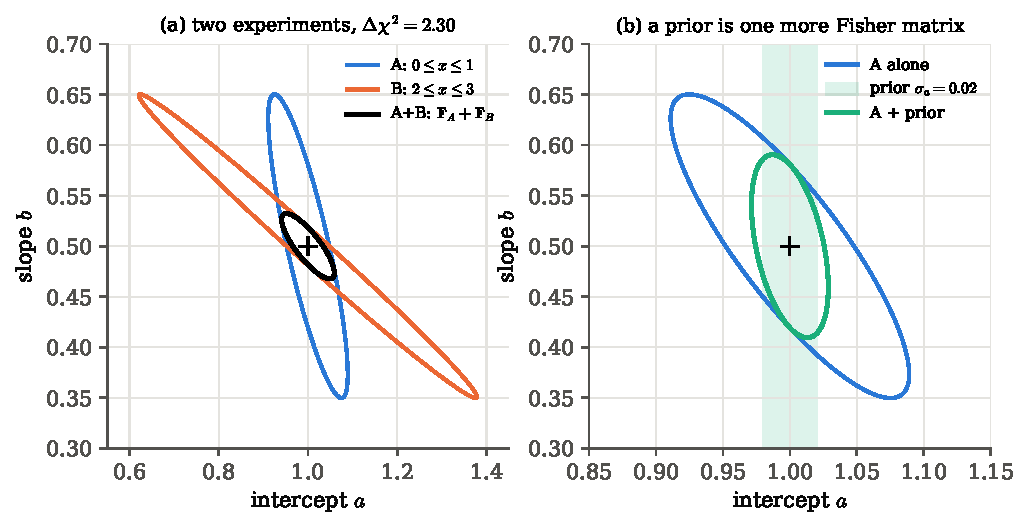
\includegraphics[width=0.98\linewidth]{figures/ch10/combine.pdf}
\caption{Left: two experiments measure the same line over different ranges of $x$; each has an elongated
$68\%$ ellipse, tilted in its own direction. The sum of their Fisher matrices gives the small black ellipse,
much smaller than either. Right: a Gaussian prior on the intercept (shaded band) is one more Fisher matrix,
and through the correlation it also shrinks the slope.}
\label{10a:fig:combine}
\end{figure}

\paragraph{Why the matrices, not the errors, are combined.} Two forecasts quoted as marginalised errors cannot be
combined by adding inverse variances: the correlations are gone, and with them the gain from crossing degeneracies.
The full Fisher matrices are kept, published and added, and marginalisation comes last.

\subsection{Changing parameters: the Jacobian sandwich}
\label{10a:sec:reparam}

The Fisher matrix is computed in the parameters the derivatives were taken with respect to, but we may want
the answer in others: $H_0$ instead of an angle, $\ln A_s$ instead of $A_s$, the pivot amplitude instead of
the intercept. Let $\bm p$ be the new parameters and $\params(\bm p)$ the old ones as functions of the new, with
Jacobian $J_{ia}=\partial\theta_i/\partial p_a$. The score transforms by the chain rule, and $\Fish$ is the
covariance of the score:
\begin{align}
  S'_a=\frac{\partial\ln\Like}{\partial p_a}
  \eqby{1}\sum_iJ_{ia}S_i,
  \qquad
  F'_{ab}=\E[S'_aS'_b]\eqby{2}\sum_{ij}J_{ia}\,\E[S_iS_j]\,J_{jb},
  \qquad
  \Fish'=\bm J\T\Fish\bm J .
  \label{10a:eq:jacobian}
\end{align}
\begin{explain}
  \item The likelihood depends on $\bm p$ only through $\params(\bm p)$.
  \item $\bm J$ is not random; take it out of the expectation.
\end{explain}
\cite{Coe2009}, eq.~(18). \emph{The covariance transforms the other way.} Inverting $\Fish'=\bm J\T\Fish\bm J$ reverses the order of the
factors: $(\Fish')^{-1}=\bm J^{-1}\Fish^{-1}\bm J^{-\mathsf T}$, with $\bm J^{-1}=\partial\bm p/\partial\params$ the Jacobian of the new
parameters with respect to the old. Read as covariances,
\[
  \Cov(\bm p)=\frac{\partial\bm p}{\partial\params}\,\Fish^{-1}\,\Bigl(\frac{\partial\bm p}{\partial\params}\Bigr)\T,
\]
which is the rule $\Cov(\bm A\params)=\bm A\Cov(\params)\bm A\T$ for a linear map, applied to the linear part of
$\bm p(\params)$ near $\params_0$. \emph{A single derived quantity.} Now let one component of $\bm p$ be a quantity
$g(\params)$ that is not one of the parameters, such as $H_0$ or $A_se^{-2\tau}$ (the other components can be any
quantities that complete the set; they do not enter its own variance). Its row of $\partial\bm p/\partial\params$ is
the gradient $\nabla g\T=(\partial_1g,\dots,\partial_mg)$, and the corresponding diagonal entry of $\Cov(\bm p)$ is
\[
  \sigma_g^2=\nabla g\T\,\Fish^{-1}\,\nabla g=\sum_{ij}\partial_ig\,(\Fish^{-1})_{ij}\,\partial_jg ,
\]
the multiparameter delta method \mainref{p.~134, Thm.~9.28} of \cref{3b:sec:invariance}. A check with two
parameters and $g=\theta_1+\theta_2$: $\nabla g=(1,1)$, so $\sigma_g^2=(\Fish^{-1})_{11}+(\Fish^{-1})_{22}+2(\Fish^{-1})_{12}$, the
familiar variance of a sum, $\Var\theta_1+\Var\theta_2+2\Cov(\theta_1,\theta_2)$. Two derived quantities $g$ and $g'$ have
covariance $\nabla g\T\Fish^{-1}\nabla g'$, an off-diagonal entry of the same matrix.\footnote{In Wasserman's Example~9.29 the result for
$\tau=\sigma/\mu$ is printed as $\frac1{\sqrt n}\sqrt{1/\hat\mu^4+\hat\sigma^2/2\hat\mu^2}$; the first term should be
$\hat\sigma^4/\hat\mu^4$, as the product of his gradient $(-\sigma/\mu^2,1/\mu)$ and his $J_n$ shows.} The
transformation is exact for the Fisher matrix, which is a local quantity at $\params_0$; whether the
transformed likelihood is still close to Gaussian is a separate question, and a nonlinear change of variables
can make it better or worse (\cref{9c:sec:line-centre}).

\paragraph{Example: the pivot as a change of variables.} For experiment~A, $a=y_p-bx_p$ and $b=b$, so
$\bm J=\bigl(\begin{smallmatrix}1&-x_p\\0&1\end{smallmatrix}\bigr)$. The new matrix $\bm J\T\Fish\bm J$ has errors
$\sigma_{y_p}=\TenCCoPivSy$, $\sigma_b=\TenCCoPivSb$ and correlation $\TenCCoPivRho$. The slope error has not
changed (the slope is the same parameter), but the amplitude is now quoted where it is measured, almost twice
better than the intercept at $x=0$.

\subsection{One number for an experiment: figures of merit}
\label{10a:sec:fom}

To rank designs, a single number helps. Hobson et al.\ list the common choices \srcref{HobsonBMC}{pp.~108--109}.
\emph{The determinant} $\det\Fish$ (``D-optimality''): the ellipsoid $\bm\delta\T\Fish\bm\delta=q$ has half-axes $\sqrt{q/\lambda_a}$
along the eigenvectors of $\Fish$, so its volume is proportional to $\prod_a\lambda_a^{-1/2}=(\det\Fish)^{-1/2}$, and a large
determinant means a small volume. \emph{The trace of $\Fish^{-1}$} (``A-optimality''): the sum of the marginalised
variances.

\emph{The information gain} measures how much the data narrow the prior, as the Kullback--Leibler divergence
\eqref{3b:eq:kl} of the posterior from the prior. Take a Gaussian prior with inverse covariance $\bm P$, so the
posterior has inverse covariance $\Fish+\bm P$ (\cref{10a:sec:priors}), and centre both at $\params_0$, as a forecast
does. With $\bm\delta=\params-\params_0$ and $\E$ the average over the posterior,
\begin{align*}
  D(\text{post},\text{prior})
  &\eqby{1}\E\bigl[\ln p_{\rm post}(\bm\delta)-\ln p_{\rm prior}(\bm\delta)\bigr]
  \\
  &\eqby{2}\tfrac12\ln\det(\Fish+\bm P)-\tfrac12\ln\det\bm P
    -\tfrac12\E\bigl[\bm\delta\T(\Fish+\bm P)\bm\delta\bigr]+\tfrac12\E\bigl[\bm\delta\T\bm P\bm\delta\bigr]
  \\
  &\eqby{3}\tfrac12\bigl[\ln\det(\Fish+\bm P)-\ln\det\bm P-\Tr\bigl(\Id-\bm P(\Fish+\bm P)^{-1}\bigr)\bigr].
\end{align*}
\begin{explain}
  \item The divergence is the average, under the first density, of the log of the ratio of the two.
  \item A Gaussian with inverse covariance $\bm M$ has $\ln p=\frac12\ln\det\bm M-\frac12\bm\delta\T\bm M\bm\delta$ plus a constant
        that is the same for both and cancels.
  \item For any matrix $\bm M$, $\E[\bm\delta\T\bm M\bm\delta]=\E\Tr(\bm M\bm\delta\bm\delta\T)=\Tr(\bm M\bm\Sigma)$ with the posterior covariance
        $\bm\Sigma=(\Fish+\bm P)^{-1}$; so the third term is $-\frac12\Tr\Id$ and the fourth $+\frac12\Tr(\bm P(\Fish+\bm P)^{-1})$.
\end{explain}
If the data say nothing, $\Fish=\bm0$ and every term vanishes; the more the data shrink the prior volume, the
larger the gain, mostly through the first two terms, which compare the two volumes.

\emph{The dark-energy figure of merit.} The equation of state of dark energy is often written
$w(a)=w_0+w_a(1-a)$ with $a$ the scale factor (cosmology notes): $w_0$ is its value today and $w_a$ how fast it
changes. The figure of merit is $1/\sqrt{\det\bm\Sigma_{w_0w_a}}$, with $\bm\Sigma_{w_0w_a}$ the marginalised $2\times2$ block of $\Fish^{-1}$.
By the half-axes of \cref{10a:sec:ellipses}, the ellipse $\Delta\chi^2=q$ has area $\pi\sqrt{q\lambda_+}\sqrt{q\lambda_-}=\pi q\sqrt{\det\bm\Sigma}$, so
the figure of merit is inversely proportional to the area of the $(w_0,w_a)$ ellipse: it is the determinant
criterion applied to that one pair.

Each number rewards a different shape: a determinant can be large for a long thin ellipse whose long axis is
useless, which is why the full matrix, not a single number, is what should be compared.

\subsection{The recipe}
\label{10a:sec:recipe}

\begin{workdef}[Fisher forecast]
\begin{enumerate}
  \item Choose the parameters and a fiducial point $\params_0$ (the forecast depends on both).
  \item Model the data: mean $\bm\mu(\params)$ and covariance $\Cmat(\params)$ of the summary the analysis will use,
        including the instrument (noise, beam, sky fraction).
  \item Differentiate the model at $\params_0$ (analytically, or by finite differences checked for stability,
        \cref{10a:sec:numderiv}).
  \item Assemble $\Fish$ by \eqref{10a:eq:gauss-fisher}, or by \eqref{10a:eq:fisher-def} for non-Gaussian data.
  \item Add the Fisher matrices of priors and of independent experiments.
  \item Transform to the parameters you want to report, $\Fish'=\bm J\T\Fish\bm J$.
  \item Invert. Marginalised errors are $\sqrt{(\Fish^{-1})_{ii}}$; $2\times2$ blocks of $\Fish^{-1}$ give ellipses at
        $\Delta\chi^2=2.30,\ 6.18$; eigenvectors give degeneracies; $\nabla g\T\Fish^{-1}\nabla g$ gives derived parameters.
  \item Check: is the predicted error small compared with the scale on which the model is nonlinear? If not,
        validate with simulations or a chain (\cref{10a:sec:cmb-check}).
\end{enumerate}
\end{workdef}
\section{Derivatives from a code that cannot differentiate}
\label{10a:sec:numderiv}

Equation \eqref{10a:eq:gauss-fisher} needs the derivative of the model with respect to each parameter. For the
CMB the model is a Boltzmann code, CAMB \cite{CAMB2000}: tens of thousands of lines that integrate the coupled
photon, baryon, neutrino and dark-matter perturbations from the early universe to today and return
$\Cell(\params)$ (the physics is in the cosmology notes; \cref{ch:T1} maps the objects). It returns numbers, not
derivatives. The only practical route is a finite difference, $[\Cell(\theta+h)-\Cell(\theta-h)]/2h$, and the
whole forecast then hangs on a number we choose by hand, the step $h$.

\paragraph{The question.} How large should the step be, and how do we know the forecast does not depend on it?
Two errors pull in opposite directions. With a large step, the model is no longer linear between
$\theta-h$ and $\theta+h$, and the difference quotient is not the derivative: a \emph{truncation error}. With a
small step, the two spectra are nearly equal, and whatever numerical noise the code has (from its finite
grids in time and wavenumber, its interpolations, its convergence tolerances) is divided by the small number
$2h$: a \emph{noise error}.

\subsection{Truncation against noise}
\label{10a:sec:numderiv-errors}

Expand $f(\theta\pm h)=f\pm hf'+\frac12h^2f''\pm\frac16h^3f'''+\frac1{24}h^4f''''\pm\frac1{120}h^5f^{(5)}+\dots$
(all derivatives at $\theta$). Then the two-point and four-point central differences are
\begin{align}
  D_2(h)\equiv\frac{f(\theta+h)-f(\theta-h)}{2h}
  &\eqby{1}f'+\frac{h^2}6f'''+\frac{h^4}{120}f^{(5)}+\dots,
  \nonumber\\
  D_4(h)\equiv\frac{4D_2(h)-D_2(2h)}3
  &\eqby{2}\frac{-f(\theta+2h)+8f(\theta+h)-8f(\theta-h)+f(\theta-2h)}{12h}
  \nonumber\\
  &\eqby{3}f'-\frac{h^4}{30}f^{(5)}+\dots
  \label{10a:eq:stencils}
\end{align}
\begin{explain}
  \item Subtract the two series: the even powers cancel; divide by $2h$.
  \item Write out $D_2(h)$ and $D_2(2h)$ and put everything over $12h$.
  \item From line (1), $D_2(2h)=f'+\frac{4h^2}6f'''+\frac{16h^4}{120}f^{(5)}$; in $4D_2(h)-D_2(2h)$ the $h^2$ terms cancel
        ($4\cdot\frac16-\frac46=0$) and the $h^4$ terms leave $\frac{4-16}{120}h^4f^{(5)}$, which divided by $3$ is
        $-h^4f^{(5)}/30$.
\end{explain}
The four-point rule is the two-point rule with its leading error extrapolated away (Richardson
extrapolation), at the price of two more model evaluations. Chapter~9 used the two-point rule to build its
emulator (\cref{9c:sec:emu-build}).

Now add noise: suppose each evaluation of $f$ carries an independent relative error of size $\epsilon$, an
absolute error of about $\epsilon\abs f$. \emph{The noise term.} In $D_2$ the two errors enter as a difference;
being independent, they add in quadrature to about $\sqrt2\,\epsilon\abs f$, and dividing by $2h$ leaves
$\epsilon\abs f/(\sqrt2\,h)$. We keep only its order, $\epsilon\abs f/h$: a factor of order one changes no scaling.
\emph{The truncation term} is the first neglected term in line~(1) of \eqref{10a:eq:stencils}, $h^2\abs{f'''}/6$. The
total error is about
\begin{equation}
  E(h)\approx\frac{\epsilon\abs f}{h}+\frac{h^2}{6}\abs{f'''},
  \qquad
  h_{\rm opt}=\Bigl(\frac{3\epsilon\abs f}{\abs{f'''}}\Bigr)^{1/3}.
  \label{10a:eq:hopt}
\end{equation}
The first term falls with $h$ and the second rises, so there is a best step in between, where the slope of $E$ is
zero:
\begin{align*}
  \frac{\dd E}{\dd h}
  &\eqby{1}-\frac{\epsilon\abs f}{h^2}+\frac{h\abs{f'''}}3=0
  \quad\Rightarrow\quad h^3=\frac{3\epsilon\abs f}{\abs{f'''}},
  \\
  \frac{\epsilon\abs f}{h_{\rm opt}}
  &\eqby{2}\frac{\epsilon^{2/3}\abs f^{2/3}\abs{f'''}^{1/3}}{3^{1/3}},
  \qquad
  \frac{h_{\rm opt}^2}6\abs{f'''}\eqby{3}\frac{3^{2/3}\epsilon^{2/3}\abs f^{2/3}\abs{f'''}^{1/3}}6 .
\end{align*}
\begin{explain}
  \item Differentiate the two terms of \eqref{10a:eq:hopt}, set the sum to zero, and multiply by $3h^2/\abs{f'''}$.
  \item Insert $1/h_{\rm opt}=(\abs{f'''}/3\epsilon\abs f)^{1/3}$ into the noise term.
  \item Insert $h_{\rm opt}^2=(3\epsilon\abs f/\abs{f'''})^{2/3}$ into the truncation term.
\end{explain}
At the optimum both terms are of order $\epsilon^{2/3}$ (the noise term is exactly twice the truncation term): a
code accurate to one part in $10^6$ gives derivatives accurate to about one part in $10^4$, not $10^6$.

\emph{The four-point rule.} Its noise term is again of order $\epsilon\abs f/h$ (the weights $1,8,8,1$ over $12h$ add
in quadrature to $\sqrt{130}/12\approx0.95$ times $\epsilon\abs f/h$), and its truncation term is $h^4\abs{f^{(5)}}/30$ from line~(3)
of \eqref{10a:eq:stencils}. So $E_4(h)\approx\epsilon\abs f/h+h^4\abs{f^{(5)}}/30$; setting
$\dd E_4/\dd h=-\epsilon\abs f/h^2+\frac4{30}h^3\abs{f^{(5)}}=0$ gives $h^5=\frac{30}4\,\epsilon\abs f/\abs{f^{(5)}}$, so
$h_{\rm opt}\propto\epsilon^{1/5}$, and the error $\epsilon\abs f/h_{\rm opt}$ is of order $\epsilon/\epsilon^{1/5}=\epsilon^{4/5}$: larger steps,
and better derivatives.

\paragraph{Example: a function we can differentiate by hand.} Take $f(x)=e^x\sin3x$ at $x=0.7$, whose derivative is
known exactly, and give it a simulated ``code noise'' of relative size $\epsilon=\TenDDeEps$.
\Cref{10a:fig:deriv-test} shows the error of the two rules against $h$, as the root-mean-square over
$\TenDDeNreal$ noise realisations. Without noise (dotted) the errors fall as $h^2$ and $h^4$ until double-precision
round-off takes over near $h\sim10^{-5}$ to $10^{-8}$. With noise, the two-point error is smallest at
$h=\TenDDeHoptTwo$, where \eqref{10a:eq:hopt} predicts $\TenDDeHpred$ and an error of $\TenDDeRelPred$ (measured:
$\TenDDeBestTwo$). The four-point rule is best at the larger step $\TenDDeHoptFour$, with error $\TenDDeBestFour$.
Below the optimum the error climbs as $1/h$ along the dashed line: there, making the step smaller makes the
derivative worse.

\begin{figure}[htbp]
\centering
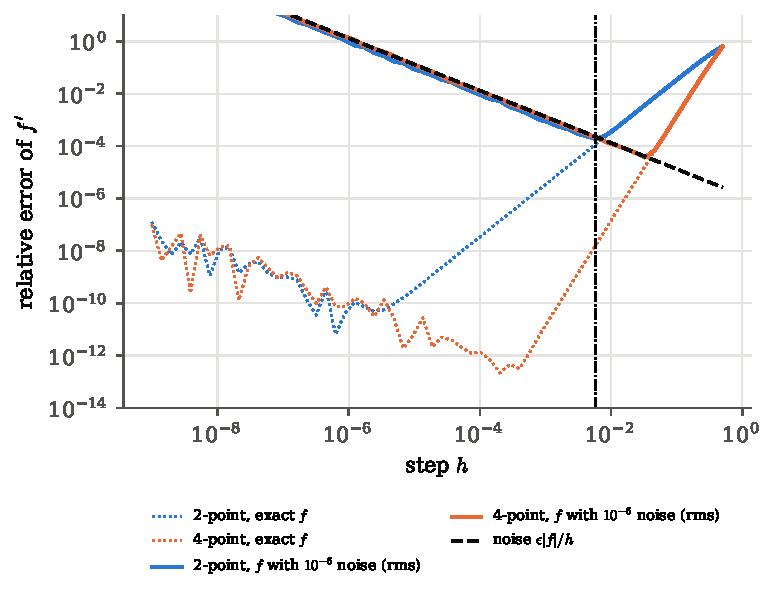
\includegraphics[width=0.7\linewidth]{figures/ch10/deriv_test.pdf}
\caption{The error of a numerical derivative of $e^x\sin3x$ against the step. Dotted: exact function values,
where only truncation and double-precision round-off act. Solid: function values with a relative noise of
$10^{-6}$; the error is the sum of a noise term rising as $1/h$ (dashed) and a truncation term falling as
$h^2$ (two-point) or $h^4$ (four-point). The vertical line is the predicted optimum of the two-point rule.}
\label{10a:fig:deriv-test}
\end{figure}

\subsection{The stability test for CAMB}
\label{10a:sec:numderiv-camb}

For CAMB we do not know $\epsilon$ or $f'''$, so we cannot compute $h_{\rm opt}$; we test instead. The steps
$h_i$ we use are roughly a third to a whole of the expected error of each parameter:
$\TenDDeStepOb$ in $\omega_b$, $\TenDDeStepOc$ in $\omega_c$, $\TenDDeStepTh$ in $100\theta_{\rm MC}$, $\TenDDeStepTau$
in $\tau$, $\TenDDeStepAs$ in $\ln(10^{10}A_s)$ and $\TenDDeStepNs$ in $n_s$. The reason for this scale is the
truncation side of \eqref{10a:eq:hopt}: the forecast is only meaningful over a region about one standard deviation
wide, so the derivative should describe the model over that region, not over a much smaller or much larger one.

The test is to multiply every step by a factor $m$, recompute the derivatives with both rules, rebuild the
forecast, and watch the marginalised errors. \pyname{04_derivatives.py} does this for
$m=\frac1{64},\frac1{16},\frac14,\frac12,1,2,4$, which takes $\TenDDeCalls$ CAMB runs, cached so that every later script
reuses them:
\pyfile[firstline=106,lastline=117,firstnumber=106]{code/ch10/04_derivatives.py}{Two- and four-point derivatives of the CMB spectra, from cached CAMB runs}
The forecast is the Planck-like temperature-and-polarization experiment of \cref{10a:sec:cmb-planck}.
\Cref{10a:fig:deriv-camb} shows the result. For $\frac14\le m\le4$ every marginalised error stays within
$\TenDDeDevFourQuarter\%$ of the four-point reference, with either rule: the forecast does not care about the
step. Below that, it does. At $m=\frac1{16}$ the largest change is $\TenDDeDevTwoSixteenth\%$; at $m=\frac1{64}$ it is
$\TenDDeDevTwoSixtyfourth\%$ (two-point) and $\TenDDeDevFourSixtyfourth\%$ (four-point), and the most affected parameter
is $\TenDDeWorstParSmall$.

\paragraph{Why the noise makes the forecast too good.} The errors at tiny steps are \emph{smaller}, not larger.
The reason is the geometric reading of \cref{10a:sec:gauss-derive}, and two parameters are enough to see it.
\emph{The Fisher matrix as dot products.} By \eqref{10a:eq:cmb-fisher}, $F_{ij}$ is a weighted sum over multipoles of
$\partial_i\Cell\,\partial_j\Cell$. Call the two derivative vectors $\bm u=(\partial_1\Cell)_\ell$ and $\bm v=(\partial_2\Cell)_\ell$, and
write $\bm a\cdot\bm b$ for the weighted sum $\sum_\ell\frac{2\ell+1}2\,a_\ell b_\ell/(\Cell+N_\ell)^2$. Then
$F_{11}=\abs{\bm u}^2$, $F_{22}=\abs{\bm v}^2$, $F_{12}=\bm u\cdot\bm v$, and by the $2\times2$ inverse of \cref{10a:sec:marginal}
the correlation of the two estimates has size $\abs\rho=\abs{\bm u\cdot\bm v}/(\abs{\bm u}\abs{\bm v})$, the cosine of the angle
between the two vectors. A degeneracy is two vectors pointing in nearly the same direction, $\abs\rho$ close to one.

\emph{Add noise.} The computed vectors are $\bm u'=\bm u+\bm n_1$ and $\bm v'=\bm v+\bm n_2$, where $\bm n_1$ and $\bm n_2$
fluctuate rapidly and randomly from one multipole to the next. A dot product of such a vector with a smooth one,
or with another independent noise vector, is a sum of terms of random sign that nearly cancel; the dot product of
a noise vector with itself is a sum of squares, which does not. So
\[
  F'_{11}\approx\abs{\bm u}^2+\abs{\bm n_1}^2,\qquad
  F'_{22}\approx\abs{\bm v}^2+\abs{\bm n_2}^2,\qquad
  F'_{12}\approx\bm u\cdot\bm v ,
\]
\[
  \abs{\rho'}=\frac{\abs{\bm u\cdot\bm v}}{\sqrt{(\abs{\bm u}^2+\abs{\bm n_1}^2)(\abs{\bm v}^2+\abs{\bm n_2}^2)}}
  <\frac{\abs{\bm u\cdot\bm v}}{\abs{\bm u}\abs{\bm v}}=\abs\rho .
\]
The diagonal has gained $\abs{\bm n}^2$ of spurious ``information'' and the off-diagonal has not. Both effects lower
the marginalised error $\sigma_1^{\rm marg}=1/\sqrt{F_{11}(1-\rho^2)}$ of \eqref{10a:eq:marg-cond}: $F_{11}$ grows and $1-\rho^2$ grows.
The second effect is the strong one near a degeneracy. With $\abs\rho=0.95$ and noise carrying $1\%$ of the power of
each vector, $\abs{\rho'}=0.95/1.01=0.941$, and $1/\sqrt{1-\rho^2}$ falls from $3.20$ to $2.95$; together with the factor
$1/\sqrt{1.01}$ the marginalised error drops by $8\%$, eight times the $1\%$ by which the noise changed the vectors.
So the symptom of noisy derivatives is an optimistic forecast, and it strikes first the parameters involved in
the strongest degeneracy; for us that is $\omega_c$, whose correlation with $n_s$ is the largest in the matrix
(\cref{10a:sec:cmb-degeneracies}).

\begin{figure}[htbp]
\centering
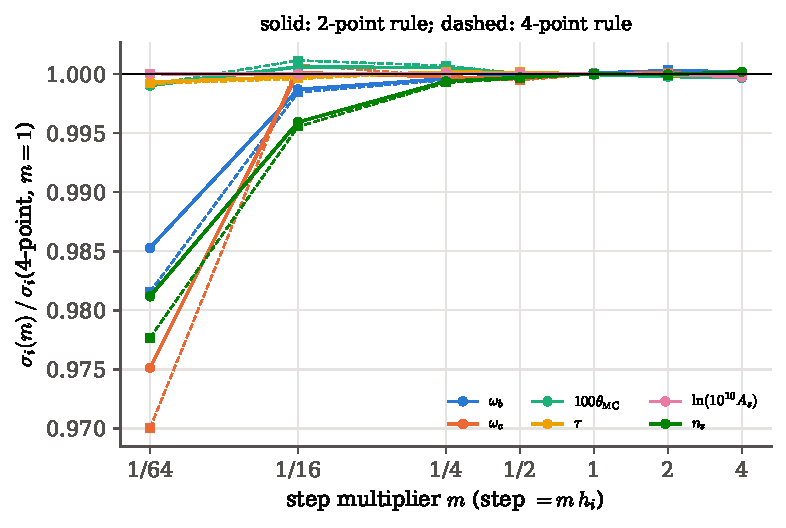
\includegraphics[width=0.7\linewidth]{figures/ch10/deriv_camb.pdf}
\caption{Marginalised errors of the six $\Lambda$CDM parameters for a Planck-like forecast, recomputed with every
derivative step multiplied by $m$, relative to the four-point rule at $m=1$. Between $m=\frac14$ and $4$ nothing
moves by more than about two tenths of a per cent. At very small steps the numerical noise of CAMB enters the
derivatives and the errors shrink by up to three per cent: noise looks like information.}
\label{10a:fig:deriv-camb}
\end{figure}

\paragraph{Rules that follow.} The two tests above turn into a short list of checks that every Fisher
forecast should pass before its numbers are believed.
\begin{enumerate}
  \item Choose steps of order a fraction of the expected error, not ``as small as possible''.
  \item Halve and double the steps; quote the forecast only if it does not move.
  \item Compare the two-point and four-point rules at the same step; agreement means truncation is negligible.
  \item If the errors drift \emph{downwards} as the steps shrink, the derivatives are noisy; raise the code's
        accuracy settings or increase the step.
  \item Differentiate quantities that are nearly linear in the parameters, such as $\ln\Cell$ in $\ln A_s$ and
        $\tau$ (\cref{9c:sec:emu-log}); the truncation error is then small at any reasonable step.
\end{enumerate}
\section{A CMB forecast for \texorpdfstring{$\Lambda$CDM}{LCDM}}
\label{10a:sec:cmb}

In 1995 the Planck satellite was a proposal. Knox \cite{Knox1995}, Jungman et al.\ \cite{Jungman1996} and Tegmark,
Taylor and Heavens \cite{TTH1997} used the machinery of the last five sections to tell the community what such a
satellite would measure, and those forecasts helped decide its design. Twenty-three years later Planck
published its final parameters \cite{Planck2018VI}. We can now do what is rarely possible with a forecast:
redo it, and compare it with what the experiment actually delivered.

\paragraph{The question.} The CMB temperature and polarization are Gaussian random fields on the sphere whose
statistics are set by the angular power spectra $\Cell^{TT}$, $\Cell^{EE}$, $\Cell^{TE}$, which a Boltzmann code computes
from the six parameters of $\Lambda$CDM (\cref{ch:T1}; the physics is in the cosmology notes). An experiment with a
given beam, noise and sky fraction will measure the $\alm$. How well will it measure the six parameters?

\subsection{From the \texorpdfstring{$\alm$}{alm} to the CMB Fisher matrix}
\label{10a:sec:cmb-derive}

\emph{The data.} Expand the measured temperature map in spherical harmonics (\cref{ch:07}). The coefficients
$\alm$ for $2\le\ell\le\ell_{\max}$, $-\ell\le m\le\ell$, are the data vector; written as real numbers there are
$2\ell+1$ of them at each $\ell$. \emph{Their mean is zero}: the parameters do not move the map, they set its
variance. \emph{Their covariance is diagonal}: statistical isotropy makes different $(\ell,m)$ uncorrelated, and the
variance of each is the sky signal plus the instrument noise,
\begin{equation}
  \langle a_{\ell m}a_{\ell'm'}\rangle=\bigl(\Cell+N_\ell\bigr)\delta_{\ell\ell'}\delta_{mm'},
  \qquad
  N_\ell=\Delta^2e^{\ell(\ell+1)\sigma_b^2},\quad\sigma_b=\frac{\mathrm{FWHM}}{\sqrt{8\ln2}} .
  \label{10a:eq:alm-cov}
\end{equation}
Here $N_\ell$ is the white noise of depth $\Delta$ (in $\mu$K\,rad) after the Gaussian beam has been divided out of
the map: the beam suppresses the signal at $\ell\gtrsim1/\sigma_b$ but not the noise, so dividing by it makes the
noise grow exponentially (\cref{ch:08}; the cosmology notes write it as $N_\ell/W_\ell$ with $W_\ell$ the beam
window). Tegmark et al.\ write the same quantity as $4\pi\sigma^2/N\,e^{\theta_b^2\ell(\ell+1)}$ for $N$ pixels of noise
$\sigma$, since $\Delta^2=\sigma^2\Omega_{\rm pix}=4\pi\sigma^2/N$ \cite{TTH1997}, eq.~(16).

\emph{Apply the Gaussian formula.} With $\bm\mu=\bm0$ only the covariance channel of \eqref{10a:eq:gauss-fisher}
survives, and $\Cmat$ is diagonal, so every matrix product is a product of diagonal entries:
\begin{align}
  F_{ij}
  &\eqby{1}\frac12\Tr\bigl[\Cmat^{-1}\Cmat_{,i}\Cmat^{-1}\Cmat_{,j}\bigr]
  \eqby{2}\frac12\sum_{\ell=2}^{\ell_{\max}}\sum_{m=-\ell}^{\ell}\frac{\partial_i\Cell}{\Cell+N_\ell}\,\frac{\partial_j\Cell}{\Cell+N_\ell}
  \eqby{3}\sum_{\ell=2}^{\ell_{\max}}\frac{2\ell+1}{2}\,\frac{\partial_i\Cell\,\partial_j\Cell}{(\Cell+N_\ell)^2} .
  \label{10a:eq:cmb-fisher}
\end{align}
\begin{explain}
  \item \eqref{10a:eq:gauss-fisher} with $\bm\mu_{,i}=\bm0$.
  \item $\Cmat^{-1}\Cmat_{,i}$ is diagonal with entry $\partial_i\Cell/(\Cell+N_\ell)$ at every $(\ell,m)$; the noise does not depend
        on the cosmological parameters.
  \item Nothing depends on $m$, so the sum over $m$ gives $2\ell+1$ equal terms.
\end{explain}
This is Tegmark, Taylor and Heavens' eq.~(18) \cite{TTH1997}, the result \cref{3b:sec:recipe-cmb} found for one
amplitude and \cref{9c:sec:emu-check} found by expanding the exact likelihood. It has a plain reading: since
$\Var\Chat=2(\Cell+N_\ell)^2/(2\ell+1)$ (cosmic variance plus noise), each multipole contributes
$(\partial_i\Cell)(\partial_j\Cell)/\Var\Chat$, the squared response of the spectrum in units of its own error bar. Multipoles
where the spectrum is precisely measured and responds strongly to $\theta_i$ dominate.

\emph{Part of the sky.} Divide the full sky into many small patches of equal area, each carrying its own
independent share of the information on the parameters. A survey that sees a fraction $\fsky$ of the sky sees the
fraction $\fsky$ of those patches. Independent pieces of data add their Fisher matrices (\cref{10a:sec:two-faces}), so
the observed part carries $\fsky$ times the Fisher matrix of the full sky: every term of \eqref{10a:eq:cmb-fisher} is
multiplied by $\fsky$, or, in the language of modes, each multipole has about $(2\ell+1)\fsky$ independent modes
instead of $2\ell+1$. The assumption is that the patches really are independent, that is, that the edge of the
mask does not couple neighbouring multipoles. A mask does couple them (\cref{ch:08}), which matters at low $\ell$,
where a mode is not small compared with the patch, and for sharp masks.

\emph{Temperature and polarization.} At each $(\ell,m)$ the data are now the pair $(a^T_{\ell m},a^E_{\ell m})$, correlated with
each other but not with other $(\ell,m)$, with the $2\times2$ covariance
$\Cmat_\ell=\bigl(\begin{smallmatrix}\Cell^{TT}+N_\ell^T&\Cell^{TE}\\ \Cell^{TE}&\Cell^{EE}+N_\ell^P\end{smallmatrix}\bigr)$. The same three steps give
\begin{equation}
  F_{ij}=\sum_\ell\frac{(2\ell+1)\fsky}{2}\Tr\bigl[\Cmat_\ell^{-1}\partial_i\Cmat_\ell\,\Cmat_\ell^{-1}\partial_j\Cmat_\ell\bigr],
  \label{10a:eq:cmb-fisher-TE}
\end{equation}
now with a $2\times2$ trace at each $\ell$. Verde \cite{Verde2010}, eqs.~(26)--(28), writes the same thing as
$\sum_\ell\partial_i\bm C_\ell\T\,\bm\Sigma_\ell^{-1}\,\partial_j\bm C_\ell$, with $\bm C_\ell=(\Cell^{TT},\Cell^{EE},\Cell^{TE})$ and $\bm\Sigma_\ell$ the $3\times3$ covariance
of the three estimated spectra. Our code implements both, and they agree to $\TenFCmChk$ in relative terms,
as they must, since they are the same Gaussian likelihood seen through two different data vectors (the
$\alm$ and the spectra built from them):
\pyfile[firstline=163,lastline=180,firstnumber=163]{code/ch10/lib_fisher10.py}{The temperature-and-polarization Fisher matrix, one $2\times2$ trace per multipole}
Lines 169--172 form the four entries of $\Cmat_\ell^{-1}\partial_i\Cmat_\ell$ for all $\ell$ at once, and line 178 is the trace of
the product of two such $2\times2$ matrices.

\emph{Several frequency channels.} Planck observed the CMB in several channels; each channel $\nu$ gives an
independent noisy measurement of the same $\alm$, with noise $N_{\ell,\nu}$. For the single ``parameter'' $\alm$ these
are independent experiments, so their Fisher informations $1/N_{\ell,\nu}$ add (\cref{10a:sec:priors}): the combined
noise is $1/N_\ell=\sum_\nu1/N_{\ell,\nu}$, the inverse-variance combination.

\subsection{Knox (1995) reproduced}
\label{10a:sec:knox}

\emph{His question.} Inflation, the brief early epoch of accelerated expansion, predicts two kinds of primordial
ripple: density fluctuations, which seed galaxies, and gravitational waves. In 1995 the anisotropy of the CMB
had just been detected on large scales, and a satellite to map it on smaller scales was being argued for. Knox
asked whether such a satellite could separate the three numbers that tell inflation models apart: the
\emph{amplitude} of the density fluctuations, their \emph{tilt} (how their strength changes with scale), and the
\emph{share of gravitational waves} in the observed anisotropy \cite{Knox1995}. If the three could not be
separated, the satellite could not test inflation, however good its maps.

\emph{His method.} Knox did not compute a Fisher matrix. He drew the estimated spectrum $\Chat$ from its
$\chi^2_{2\ell+1}$ distribution, found the maximum of the exact likelihood by simulated annealing, repeated this
$100$ times per experiment, and quoted the standard deviation of the maxima \srcref{Knox1995}{pp.~11--14}. His
Table~1 is therefore a Monte Carlo result, and a Fisher forecast should reproduce it.

\subsubsection*{His setup}

\emph{The background cosmology} is standard cold dark matter: a flat universe made of matter only, with no
cosmological constant and no reionisation. It is held fixed; only the three primordial numbers are fitted.

\emph{The density (scalar) part.} Its strength is quoted through the quadrupole it produces. Knox's $Q$ is the
root-mean-square quadrupole, defined by $Q^2=5C_2/4\pi$, so the scalar part alone has $C_2^S=4\pi Q_S^2/5$. Its
shape across multipoles, $s_\ell=\Cell^S/C_2^S$, is fixed by the background cosmology and by the tilt $n_S$; we
compute it with CAMB.

\emph{The gravitational-wave (tensor) part} adds its own spectrum, with quadrupole $C_2^T=4\pi Q_T^2/5$ and shape
$t_\ell=\Cell^T/C_2^T$. Gravitational waves decay once they come inside the horizon, so $t_\ell$ falls steeply above
$\ell\sim100$ and the tensor part only shows on large scales. Its strength is measured against the scalar
part by the ratio of the two quadrupoles, $r=Q_T^2/Q_S^2=C_2^T/C_2^S$. The tensor tilt $n_T$ is held at its fiducial
value.

\begin{center}
\small
\renewcommand{\arraystretch}{1.15}
\begin{tabular}{@{}lll@{}}
\toprule
quantity & meaning & value\\\midrule
$h$ & Hubble constant$/(100$ km\,s$^{-1}$\,Mpc$^{-1})$ & $0.5$\\
$\Omega$ & total density$/$critical; no $\Lambda$ & $1$\\
$\Omega_bh^2$ & physical baryon density & $0.0125$\\
$n_S$ & scalar tilt (fitted) & $0.94$\\
$n_T$ & tensor tilt (fixed) & $-0.04$\\
$r$ & tensor/scalar quadrupole ratio (fitted) & $0.28$\\
$Q_S$ & scalar rms quadrupole (fitted) & $20\,\mu$K\\
\bottomrule
\end{tabular}
\end{center}
These are Knox's fiducial values, from chaotic inflation \srcref{Knox1995}{pp.~3--5}.

\subsubsection*{His key equations, derived}

\emph{The model spectrum.} The two parts are independent, so their spectra add, and each is its quadrupole
times its shape:
\begin{align}
  \Cell
  &\eqby{1}\Cell^S+\Cell^T
   \eqby{2}C_2^S\,s_\ell+C_2^T\,t_\ell
   \eqby{3}C_2^S\bigl[s_\ell(n_S)+r\,t_\ell\bigr]
  \nonumber\\
  &\eqby{4}\frac{4\pi}5Q_S^2\bigl[s_\ell(n_S)+r\,t_\ell\bigr],
  \qquad s_\ell=\frac{\Cell^S}{C_2^S},\quad t_\ell=\frac{\Cell^T}{C_2^T}.
  \label{10a:eq:knox-model}
\end{align}
\begin{explain}
  \item Uncorrelated contributions to the $\alm$ add their variances.
  \item The definitions of the two shapes.
  \item $C_2^T=r\,C_2^S$, the definition of $r$.
  \item $C_2^S=4\pi Q_S^2/5$, from $Q^2=5C_2/4\pi$.
\end{explain}
\emph{The derivatives} follow at once. $\Cell$ is proportional to $Q_S^2$, so $\partial_{Q_S}\Cell=2\Cell/Q_S$; it is linear in
$r$, so $\partial_r\Cell=\frac{4\pi}5Q_S^2t_\ell$; and $n_S$ enters only through the shape, so $\partial_{n_S}\Cell=\frac{4\pi}5Q_S^2\,\partial_{n_S}s_\ell$, which
we take from a cubic spline in $n_S$ of $\ln s_\ell$ computed with CAMB on a grid of tilts. As a check of the shapes,
our $t_{55}/s_{55}$ is $\TenEKnTSratio$, against Knox's ``$C^T_{55}/C^S_{55}\simeq r/3$''.

\emph{His experiments.} Full sky, Gaussian beams of FWHM $20'$, $30'$ and $40'$, and noise described by a weight per
solid angle $w$, with $w^{-1/2}=15$ or $30\,\mu$K\,deg. His equation~(4) gives the variance of the estimated spectrum,
\[
  \Var\Chat=\frac2{2\ell+1}\bigl(\Cell+w^{-1}e^{\ell^2\sigma_b^2}\bigr)^2 .
\]
We derive it. At each $\ell$ the estimate is the average power of the $2\ell+1$ real coefficients,
$\Chat=\frac1{2\ell+1}\sum_m\abs{\alm}^2$, and by \eqref{10a:eq:alm-cov} each coefficient is an independent Gaussian of mean zero
and variance $\Cell+N_\ell$. Then
\begin{align*}
  \Chat
  &\eqby{1}\frac{\Cell+N_\ell}{2\ell+1}\sum_m\Bigl(\frac{\alm}{\sqrt{\Cell+N_\ell}}\Bigr)^2
   \eqby{2}\frac{\Cell+N_\ell}{2\ell+1}\,\chi^2_{2\ell+1},
  \\
  \Var\Chat&\eqby{3}\frac{(\Cell+N_\ell)^2}{(2\ell+1)^2}\,2(2\ell+1)=\frac{2(\Cell+N_\ell)^2}{2\ell+1}.
\end{align*}
\begin{explain}
  \item Divide and multiply each term by the variance.
  \item The bracket is a standard normal, and the sum of $2\ell+1$ independent squared standard normals is
        $\chi^2_{2\ell+1}$ (\cref{3b:sec:recipe-cmb}).
  \item A $\chi^2_k$ variable has variance $2k$; a constant factor comes out squared.
\end{explain}
This is his (4) with $N_\ell=w^{-1}e^{\ell^2\sigma_b^2}$. Comparing with \eqref{10a:eq:alm-cov}, $N_\ell=\Delta^2e^{\ell(\ell+1)\sigma_b^2}$, his
$w^{-1}$ plays the part of our $\Delta^2$, and he writes $\ell^2$ for $\ell(\ell+1)$, which differ by less than $1\%$ where the
beam matters. The two noise levels are the same physical quantity, the pixel noise variance times the pixel
solid angle, in different units. Knox quotes $w^{-1/2}$ in $\mu$K\,deg; we need $\Delta$ in $\mu$K\,rad. One degree is
$\pi/180$ radians, so $w^{-1/2}=15\,\mu$K\,deg is $\Delta=15\times\pi/180=0.262\,\mu$K\,rad and $\Delta^2=0.0685\,\mu$K$^2$\,sr; with
that conversion $\Delta^2=w^{-1}$. His Fisher matrix is therefore \eqref{10a:eq:cmb-fisher} with $\fsky=1$.

\emph{Symbol map.} Knox's symbols and ours:
\begin{center}
\small
\renewcommand{\arraystretch}{1.1}
\begin{tabular}{@{}lll@{}}
\toprule
Knox & ours & meaning\\\midrule
$C_\ell$, $C_\ell^S$, $C_\ell^T$ & $\Cell$, $\Cell^S$, $\Cell^T$ & total, scalar, tensor spectra\\
$Q_S$, $Q_T$ & $(5C_2^S/4\pi)^{1/2}$, $(5C_2^T/4\pi)^{1/2}$ & rms quadrupoles\\
$w^{-1}$ & $\Delta^2$ & white-noise level, $\mu$K$^2$\,sr\\
$\sigma_b$ & $\sigma_b=\mathrm{FWHM}/\sqrt{8\ln2}$ & beam width\\
$\ell_*$, $\bar Q_S$ & $\ell_*$, $\bar Q_S$ & pivot multipole, amplitude at the pivot\\
\bottomrule
\end{tabular}
\end{center}

\subsubsection*{The pivot}

\emph{The question.} Knox's amplitude and tilt came out almost perfectly correlated, and he explained why:
the spectrum is measured best around some multipole $\ell_*$, and a change of tilt can be compensated by a change
of amplitude that keeps the power at $\ell_*$ fixed. So he quoted the amplitude at the pivot,
$\bar Q_S=Q_S(\ell_*/2)^{(n_S-0.94)/2}$, chosen so that it is uncorrelated with $n_S$ \srcref{Knox1995}{pp.~12--13}. Where does
that formula come from, and which $\ell_*$ is it?

\emph{Why the amplitude at a pivot absorbs the tilt.} A tilt $n_S$ different from the fiducial $0.94$ multiplies the
primordial power at wavenumber $k$ by $(k/k_2)^{n_S-0.94}$, where $k_2$ is the wavenumber the quadrupole sees and
where the shape is normalised. Multipole $\ell$ sees mostly $k\approx\ell/D_*$ (\cref{8a:sec:lit-pivot}, Step~2), so
$k/k_2\approx\ell/2$ and, to that approximation, $s_\ell(n_S)=s_\ell(0.94)\,(\ell/2)^{n_S-0.94}$. The scalar spectrum is then
\begin{align*}
  \Cell^S
  &\eqby{1}\frac{4\pi}5Q_S^2\Bigl(\frac\ell2\Bigr)^{n_S-0.94}s_\ell(0.94)
  \\
  &\eqby{2}\frac{4\pi}5\Bigl[Q_S^2\Bigl(\frac{\ell_*}2\Bigr)^{n_S-0.94}\Bigr]\Bigl(\frac\ell{\ell_*}\Bigr)^{n_S-0.94}s_\ell(0.94)
  \\
  &\eqby{3}\frac{4\pi}5\,\bar Q_S^2\Bigl(\frac\ell{\ell_*}\Bigr)^{n_S-0.94}s_\ell(0.94).
\end{align*}
\begin{explain}
  \item The scalar part of \eqref{10a:eq:knox-model} with the tilted shape.
  \item Split $(\ell/2)=(\ell_*/2)(\ell/\ell_*)$ and group the factor that does not depend on $\ell$ with $Q_S^2$.
  \item Name the bracket $\bar Q_S^2$; its square root is Knox's $\bar Q_S=Q_S(\ell_*/2)^{(n_S-0.94)/2}$.
\end{explain}
Written this way, a change of tilt rotates the spectrum about $\ell=\ell_*$, where $(\ell/\ell_*)^{n_S-0.94}=1$, and leaves
the power there equal to $\frac{4\pi}5\bar Q_S^2s_{\ell_*}$. So $\bar Q_S$ is the amplitude referred to $\ell_*$ instead of to the
quadrupole, the move of the reference point that \cref{8a:sec:lit-pivot} made for $A_s$ with \eqref{8a:eq:pivot-shift}.

\emph{Which $\ell_*$.} Taking logarithms, $\ln\bar Q_S=\ln Q_S+\frac12(n_S-0.94)\ln(\ell_*/2)$, and requiring zero
covariance with $n_S$,
\begin{align}
  0=\Cov(\ln\bar Q_S,n_S)
  &\eqby{1}\Cov(\ln Q_S,n_S)+\tfrac12\ln(\ell_*/2)\Var(n_S)
  \ \Rightarrow\
  \ln\frac{\ell_*}2=-\frac{2\Cov(\ln Q_S,n_S)}{\Var(n_S)},
  \nonumber\\
  \Var(\ln\bar Q_S)&\eqby{2}\Var(\ln Q_S)-\frac{\Cov(\ln Q_S,n_S)^2}{\Var(n_S)} ,
  \label{10a:eq:pivot}
\end{align}
\begin{explain}
  \item Covariance is linear in each argument; the term $-0.94$ is a constant.
  \item Expand $\Var(\ln Q_S+c\,n_S)$ with $c=\frac12\ln(\ell_*/2)$ and insert the value of $c$: this is the Schur complement
        \eqref{10a:eq:schur} once more, the variance of $\ln Q_S$ with the part explained by $n_S$ removed.
\end{explain}
with all variances and covariances taken from $\Fish^{-1}$. This is \eqref{8a:eq:kdec} in Knox's variables.

\emph{The pivot is an information-weighted mean.} Leave aside the tensor part, which is small where most of the
information lies, and use the tilted shape above. Then $\partial\Cell/\partial\ln Q_S=2\Cell$ and $\partial\Cell/\partial n_S=\Cell\ln(\ell/2)$. Each
multipole enters the Fisher sum \eqref{10a:eq:cmb-fisher} with the factor $\frac{2\ell+1}2(\Cell+N_\ell)^{-2}$; call
$\mathcal I_\ell=\frac{2\ell+1}2\bigl[\Cell/(\Cell+N_\ell)\bigr]^2$ the information of multipole $\ell$ and $g_\ell=\ln(\ell/2)$. Then
$F_{QQ}=4\sum\mathcal I_\ell$, $F_{Qn}=2\sum\mathcal I_\ell g_\ell$, $F_{nn}=\sum\mathcal I_\ell g_\ell^2$, and
\[
  \ln\frac{\ell_*}2
  \eqby{1}-\frac{2\Cov(\ln Q_S,n_S)}{\Var(n_S)}
  \eqby{2}\frac{2F_{Qn}}{F_{QQ}}
  \eqby{3}\frac{\sum_\ell\mathcal I_\ell\ln(\ell/2)}{\sum_\ell\mathcal I_\ell},
\]
\begin{explain}
  \item \eqref{10a:eq:pivot}.
  \item The $2\times2$ inverse \eqref{10a:eq:inv22}: $\Cov=-F_{Qn}/\det\Fish$, $\Var(n_S)=F_{QQ}/\det\Fish$; the determinant cancels.
  \item Insert the two sums; the factors $2\cdot2/4$ cancel.
\end{explain}
Adding $\ln2$ to both sides, $\ln\ell_*=\sum_\ell\mathcal I_\ell\ln\ell\big/\sum_\ell\mathcal I_\ell$: $\ln\ell_*$ is the mean of $\ln\ell$ over the multipoles, each weighted by the information it carries, as
\cref{8a:sec:lit-pivot} found for Planck's $k_*$. The straight-line pivot of \cref{10a:sec:degeneracy} is the same
statement with $x$ in place of $\ln\ell$. Our numbers below keep the tensor part and the exact shapes, so the
pivots in \cref{10a:tab:knox} come from \eqref{10a:eq:pivot} with the full $\Fish^{-1}$.

\subsubsection*{What we compute, side by side, and why the numbers differ}

\emph{What we compute.} \pyname{05_knox1995.py} builds $s_\ell$ and $t_\ell$ with CAMB for Knox's cosmology, forms the
three derivatives above, sums \eqref{10a:eq:cmb-fisher} with $\fsky=1$ and Knox's noise for each of his six experiments,
inverts, and applies \eqref{10a:eq:pivot}. To test the Fisher matrix against his own procedure, it also repeats
that procedure for the first experiment with $\TenEKnNsim$ simulations instead of $100$: draw $\Chat$, maximise the
exact likelihood, take the scatter of the maxima.

\emph{Side by side.} \Cref{10a:tab:knox} and \cref{10a:fig:knox} put the numbers together. The pivot of the first
experiment is at $\ell_*=\TenEKnOnePiv$; Knox reports $\ell_*=210$ for it \srcref{Knox1995}{p.~13}. Our $\TenEKnNsim$ simulations give
$\sigma(n_S)=\TenEKnMCSn$, $\sigma(r)=\TenEKnMCSr$, $\sigma(\bar Q_S)/\bar Q_S=\TenEKnMCSq$, with pivot $\TenEKnMCPiv$, all equal to the Fisher
values within the $\pm\TenEKnErr\%$ simulation error, and no bias (mean $\hat n_S=\TenEKnMCMeanN$, $\hat r=\TenEKnMCMeanR$). So for this
model the Fisher matrix is an accurate description of maximum likelihood.

\emph{Why they differ: the tilt and the amplitude.} Knox's numbers are standard deviations of $N=100$ values, and
a standard deviation estimated from $N$ Gaussian values has a relative error of $1/\sqrt{2(N-1)}=1/\sqrt{198}=7\%$. Of
the twelve tilt and amplitude entries, nine agree with ours within that $7\%$ and the other three (the tilt of the
first experiment, $0.016$ against $\TenEKnOneSn$, and two amplitudes) within $14\%$, two sampling errors: about what
twelve comparisons with $7\%$ noise should produce. Nothing beyond sampling noise is needed to explain them.

\emph{Why they differ: the tensor ratio.} Here our Fisher errors equal Knox's own analytic estimates ($0.10$,
$0.14$, $0.12$, $0.19$, $0.16$, $0.22$) but sit below his simulations by factors of $1.22$ to $1.29$ for five
experiments and $1.83$ for the last, far more than the $7\%$ sampling error. One candidate is a constraint $r\ge0$
on the fits. Its effect can be computed. If the fits that want $r<0$ are set to $r=0$, the scatter of $\hat r$ is that
of a Gaussian cut off at zero. For a Gaussian of mean $\mu$ and unit width, the cut-off variable $Y=\max(X,0)$ has
$\E Y=\mu\Phi(\mu)+\varphi(\mu)$ and $\E Y^2=(\mu^2+1)\Phi(\mu)+\mu\varphi(\mu)$, with $\Phi$ and $\varphi$ the standard normal
distribution and density (integrate $y$ and $y^2$ against the Gaussian over $y>0$). For $r/\sigma_r=\mu=1$ this gives a
standard deviation $0.87\,\sigma_r$, for $\mu=2$ it gives $0.98\,\sigma_r$; discarding those fits instead gives $0.79$ and
$0.94$. A constraint $r\ge0$ therefore makes the scatter \emph{smaller}, and cannot by itself produce an excess of
$20$ to $80\%$. The cause is not stated in Knox's paper, and we have not found it. A maximiser that sometimes
stops short of the maximum would add scatter of the right sign, but that is a guess we have not tested.

\emph{Lesson.} Where the likelihood is close to Gaussian, as for the tilt and the pivot amplitude, a few lines
of Fisher algebra reproduce a hundred simulated annealings per experiment; where a forecast and a simulation
disagree, rerunning the simulation more carefully, as our $\TenEKnNsim$ fits did, decides which one to trust.

\begin{table}[htbp]
\centering
\small
\renewcommand{\arraystretch}{1.15}
\begin{tabular}{@{}cc ccc ccc c@{}}
\toprule
 & & \multicolumn{3}{c}{Knox 1995, 100 simulations} & \multicolumn{3}{c}{Fisher (ours)} & \\
\cmidrule(lr){3-5}\cmidrule(lr){6-8}
FWHM & $w^{-1/2}$ & $\sigma(\bar Q_S)/\bar Q_S$ & $\sigma(n_S)$ & $\sigma(r)$ & $\sigma(\bar Q_S)/\bar Q_S$ & $\sigma(n_S)$ & $\sigma(r)$ & $\ell_*$\\\midrule
$20'$ & 15 & 0.0027 & 0.016 & 0.11 & $\TenEKnOneSq$ & $\TenEKnOneSn$ & $\TenEKnOneSr$ & $\TenEKnOnePiv$\\
$20'$ & 30 & 0.0041 & 0.029 & 0.18 & $\TenEKnTwoSq$ & $\TenEKnTwoSn$ & $\TenEKnTwoSr$ & $\TenEKnTwoPiv$\\
$30'$ & 15 & 0.0028 & 0.022 & 0.14 & $\TenEKnThreeSq$ & $\TenEKnThreeSn$ & $\TenEKnThreeSr$ & $\TenEKnThreePiv$\\
$30'$ & 30 & 0.0047 & 0.044 & 0.23 & $\TenEKnFourSq$ & $\TenEKnFourSn$ & $\TenEKnFourSr$ & $\TenEKnFourPiv$\\
$40'$ & 15 & 0.0035 & 0.034 & 0.19 & $\TenEKnFiveSq$ & $\TenEKnFiveSn$ & $\TenEKnFiveSr$ & $\TenEKnFivePiv$\\
$40'$ & 30 & 0.0050 & 0.058 & 0.42 & $\TenEKnSixSq$ & $\TenEKnSixSn$ & $\TenEKnSixSr$ & $\TenEKnSixPiv$\\\midrule
\multicolumn{2}{@{}l}{ours, $\TenEKnNsim$ sims, $20'/15$} & & & & $\TenEKnMCSq$ & $\TenEKnMCSn$ & $\TenEKnMCSr$ & $\TenEKnMCPiv$\\
\bottomrule
\end{tabular}
\caption{Knox's Table~1 (``numerical'' columns, $w^{-1/2}$ in $\mu$K\,deg) against the Fisher forecast for the same model
and experiments, and against our own repetition of his simulation for the first experiment. $\ell_*$ is the pivot
multipole of \eqref{10a:eq:pivot}.}
\label{10a:tab:knox}
\end{table}

\begin{figure}[htbp]
\centering
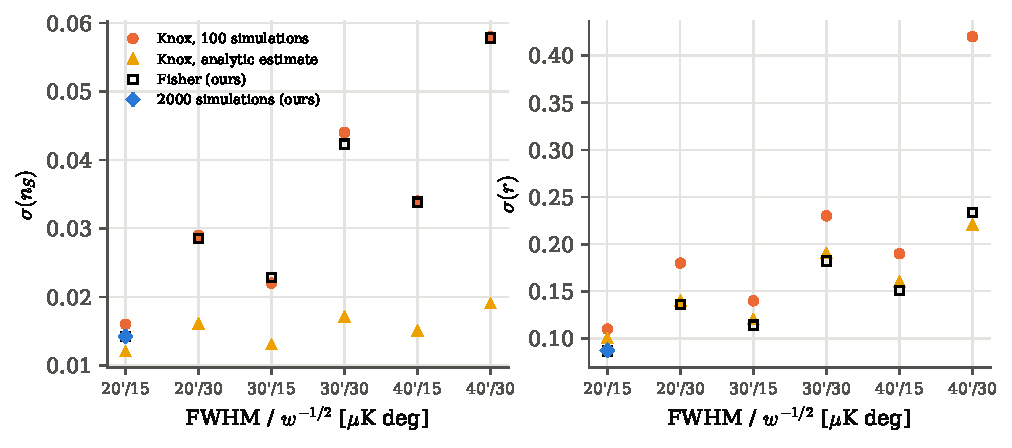
\includegraphics[width=0.98\linewidth]{figures/ch10/knox_table.pdf}
\caption{Knox's forecasts redone. Circles: Knox's $100$-simulation errors; triangles: his analytic estimates;
open squares: our Fisher matrix; diamond: our $2000$ simulated experiments for the first configuration. The
Fisher matrix reproduces his simulations for the tilt (left) and his analytic estimates for the tensor
ratio (right).}
\label{10a:fig:knox}
\end{figure}

\begin{figure}[htbp]
\centering
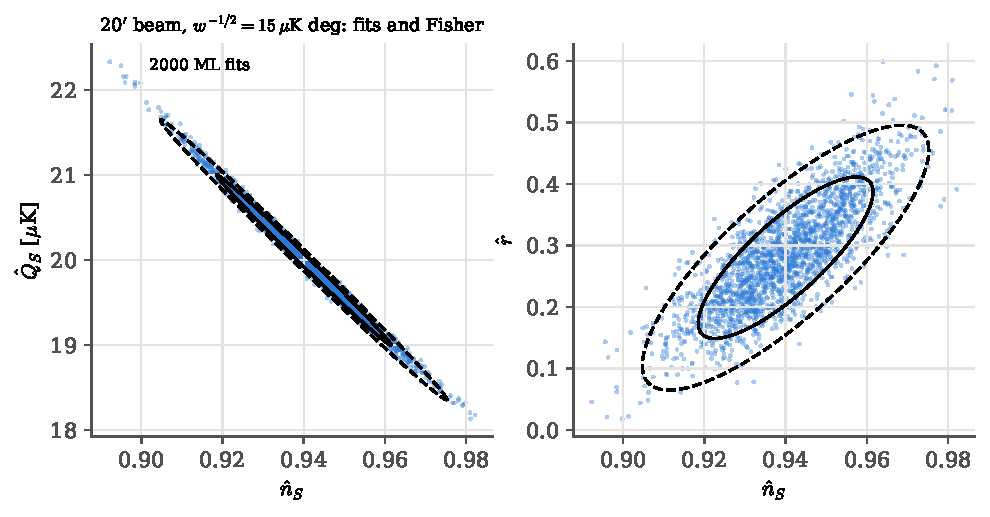
\includegraphics[width=0.98\linewidth]{figures/ch10/knox_mle.pdf}
\caption{Our $2000$ maximum-likelihood fits for Knox's $20'$, $15\,\mu$K\,deg experiment, with the Fisher ellipses
($\Delta\chi^2=2.30$ solid, $6.18$ dashed). Left: amplitude and tilt are almost perfectly anticorrelated, the
lever-arm degeneracy that the pivot removes. Right: the tilt and the tensor ratio.}
\label{10a:fig:knox-mle}
\end{figure}

\subsection{A Planck-like forecast against Planck 2018}
\label{10a:sec:cmb-planck}

\emph{Their question.} The final Planck release set out to give the definitive values of the six parameters of
$\Lambda$CDM from the full mission's temperature and polarization maps \cite{Planck2018VI}. Several of those numbers
carried questions of their own. Whether the tilt $n_s$ is below one, and by how much, tests inflation, which
predicts a slightly red spectrum. The optical depth $\tau$ dates reionisation, and through the degeneracy described
in \cref{10a:sec:cmb-degeneracies} it limits how well the primordial amplitude is known. And the Hubble constant
derived from the CMB, $67.36\pm0.54$ once the CMB lensing spectrum is added (the $0.60$ of
\cref{10a:tab:planck} is without it), is set against the $73.04\pm1.04$ of the supernova distance ladder: the
Hubble tension of \cref{T2b:sec:tension}. Each question needs an error bar that can
be trusted, which is what makes the comparison with a forecast interesting.

\emph{Their parameters, one at a time.} Planck samples in a basis chosen to be close to what the spectrum
measures directly, $\params=(\omega_b,\omega_c,100\theta_{\rm MC},\tau,\ln(10^{10}A_s),n_s)$.
The \emph{physical baryon density} $\omega_b=\Omega_bh^2$ sets how strongly the photon--baryon fluid is loaded, which
shows as the alternating heights of odd and even acoustic peaks. The \emph{physical cold-dark-matter density}
$\omega_c=\Omega_ch^2$ sets the epoch of matter--radiation equality and so the overall heights of the first peaks.
The \emph{angle} $100\theta_{\rm MC}$ is an approximation to the angular size of the sound horizon at last scattering
($\theta_*=r_*/D_M$ in the cosmology notes); it fixes the positions of the peaks. The \emph{optical depth} $\tau$ to
reionisation suppresses all but the largest scales by $e^{-2\tau}$. The \emph{amplitude} $\ln(10^{10}A_s)$ and the
\emph{tilt} $n_s$ describe the primordial spectrum at the pivot $k=0.05\,$Mpc$^{-1}$ (\cref{8a:sec:lit-pivot}): its overall
height, and how its height changes from large scales to the damping tail. The fiducial model is the Planck 2018
best fit used throughout the book:
\begin{center}
\small
\renewcommand{\arraystretch}{1.15}
\begin{tabular}{@{}cccccc|c@{}}
\toprule
$\omega_b$ & $\omega_c$ & $100\theta_{\rm MC}$ & $\tau$ & $\ln(10^{10}A_s)$ & $n_s$ & $H_0$ (derived)\\\midrule
$0.02237$ & $0.1200$ & $\approx1.041$ & $0.0544$ & $3.044$ & $0.9649$ & $\TenFCmHzFid$\\
\bottomrule
\end{tabular}
\end{center}
$H_0$ is not in the basis; it follows from the other parameters.

\emph{Where we have met $H_0$ before.} In \cref{3b:sec:hubble} $H_0$ was fitted to mock supernovae made with $H_0=70$, its error was the Cram\'er--Rao bound from a Fisher matrix, and that matrix turned singular once the candle's absolute magnitude $M$ was left free. The inverse ladder of \cref{T2b:sec:bao} took the sound horizon $r_d=147.09$\,Mpc from the CMB and turned DESI's $hr_d$ into $H_0=69.2\pm0.9$. The chain of \cref{9c:sec:planck} sampled $H_0$ directly from one simulated temperature spectrum and found $67.06\pm0.93$. What is the same here is the Fisher matrix as the error of an efficient estimator, and the experiment class of that chain: the forecast below for the chain's own one-channel experiment gives $0.93$ again. What is different is that no data are fitted at all. The centre is the fiducial $\TenFCmHzFid$ by construction, and only the width is predicted; $H_0$ is not a parameter but a function of $\omega_b$, $\omega_c$ and $100\theta_{\rm MC}$, its error carried by the delta method of \cref{10a:sec:reparam}; and the scale is set by the sound horizon at last scattering, a cousin of the $r_d$ of the inverse ladder, not by a candle calibrated nearby. The forecast for Planck's three channels is tighter than that chain, $\TenFCmPttHz$ against $0.93$, because three channels carry less noise than one, and it is tighter than Planck's own $0.92$ because it leaves out the foregrounds and calibrations whose cost is traced below.

\emph{Their instrument, in our model.} Planck's cosmological information at high $\ell$ comes from three frequency
channels. We describe each by its beam and its white-noise level \cite{Planck2018I}, Table~4, and combine them by
inverse variance as in \cref{10a:sec:cmb-derive}:
\begin{center}
\small
\renewcommand{\arraystretch}{1.15}
\begin{tabular}{@{}cccc@{}}
\toprule
channel & beam FWHM & temperature noise & polarization noise\\\midrule
100\,GHz & $9.66'$ & $1.29\,\mu$K\,deg & $1.96\,\mu$K\,deg\\
143\,GHz & $7.22'$ & $0.55\,\mu$K\,deg & $1.17\,\mu$K\,deg\\
217\,GHz & $4.90'$ & $0.78\,\mu$K\,deg & $1.75\,\mu$K\,deg\\
\bottomrule
\end{tabular}
\end{center}
Two forecasts are made. ``PTT'' uses the temperature spectrum at $2\le\ell\le2500$ on $\fsky=\TenFCmFsky$. ``PTE'' adds
$E$-mode polarization at $30\le\ell\le2000$ through \eqref{10a:eq:cmb-fisher-TE}. Both have a Gaussian prior
$\sigma_\tau=0.0086$ standing in for Planck's low-$\ell$ polarization likelihood (lowE), which on its own measures $\tau$
to that precision \cite{Planck2018VI}. The derivatives are the four-point ones of \cref{10a:sec:numderiv}.

\emph{What Planck fitted, and how it relates to our formula.} Above $\ell=30$ Planck's likelihood is a Gaussian in
the binned cross-spectra $\hat{\bm C}$ of the frequency maps, with a covariance $\bm\Sigma$ computed once for a fiducial
model (\cref{9c:sec:hl}):
\[
  -2\ln\Like=\bm\Delta\T\bm\Sigma^{-1}\bm\Delta+\text{const},\qquad \bm\Delta=\hat{\bm C}-\bm C(\params,\bm\nu).
\]
The model $\bm C(\params,\bm\nu)$ is the CMB spectrum plus foregrounds and calibrations, controlled by about twenty
nuisance parameters $\bm\nu$; below $\ell=30$ separate likelihoods handle temperature and lowE. This is a Gaussian
with fixed covariance, so only the mean channel of \eqref{10a:eq:gauss-fisher} survives, and its Fisher matrix is
$F_{ij}=\partial_i\bm C\T\bm\Sigma^{-1}\partial_j\bm C$. Leave out the nuisances, bins and cross-spectra, take $\bm\Sigma$ to be the Gaussian
covariance of the estimated spectra, and this is Verde's form, which agrees with \eqref{10a:eq:cmb-fisher-TE}.
So our forecast is Planck's likelihood without its nuisance parameters. Putting them back adds rows and
columns to $\Fish$, and marginalising over them can only enlarge the errors (\cref{10a:sec:marginal}); we should
expect our numbers to be optimistic, and the question is by how much.

\begin{table}[htbp]
\centering
\small
\renewcommand{\arraystretch}{1.2}
\begin{tabular}{@{}l ccc ccc c@{}}
\toprule
 & \multicolumn{3}{c}{TT + lowE} & \multicolumn{3}{c}{TT,TE,EE + lowE} & S4-like\\
\cmidrule(lr){2-4}\cmidrule(lr){5-7}\cmidrule(lr){8-8}
 & Planck 2018 & ours & ratio & Planck 2018 & ours & ratio & ours\\\midrule
$\omega_b$ & 0.00022 & $\TenFCmPttOb$ & $\TenFCmRatTTOb$ & 0.00015 & $\TenFCmPteOb$ & $\TenFCmRatTEOb$ & $\TenFCmSfOb$\\
$\omega_c$ & 0.0021 & $\TenFCmPttOc$ & $\TenFCmRatTTOc$ & 0.0014 & $\TenFCmPteOc$ & $\TenFCmRatTEOc$ & $\TenFCmSfOc$\\
$100\theta_{\rm MC}$ & 0.00047 & $\TenFCmPttTh$ & $\TenFCmRatTTTh$ & 0.00031 & $\TenFCmPteTh$ & $\TenFCmRatTETh$ & $\TenFCmSfTh$\\
$\tau$ & 0.0080 & $\TenFCmPttTau$ & $\TenFCmRatTTTau$ & 0.0076 & $\TenFCmPteTau$ & $\TenFCmRatTETau$ & $\TenFCmSfTau$\\
$\ln(10^{10}A_s)$ & 0.016 & $\TenFCmPttAs$ & $\TenFCmRatTTAs$ & 0.016 & $\TenFCmPteAs$ & $\TenFCmRatTEAs$ & $\TenFCmSfAs$\\
$n_s$ & 0.0057 & $\TenFCmPttNs$ & $\TenFCmRatTTNs$ & 0.0044 & $\TenFCmPteNs$ & $\TenFCmRatTENs$ & $\TenFCmSfNs$\\\midrule
$H_0$ & 0.92 & $\TenFCmPttHz$ & & 0.60 & $\TenFCmPteHz$ & & $\TenFCmSfHz$\\
$\Omega_m$ & 0.013 & $\TenFCmPttOm$ & & 0.0084 & $\TenFCmPteOm$ & & $\TenFCmSfOm$\\
$\Omega_mh^3$ & 0.00046 & $\TenFCmPttOmhThree$ & & 0.00029 & $\TenFCmPteOmhThree$ & & $\TenFCmSfOmhThree$\\
$10^9A_se^{-2\tau}$ & 0.014 & $\TenFCmPttAsE$ & & 0.012 & $\TenFCmPteAsE$ & & $\TenFCmSfAsE$\\
\bottomrule
\end{tabular}
\caption{Marginalised $1\sigma$ errors: Planck 2018 \cite{Planck2018VI}, Table~2, against our Fisher forecast for the
same data combination (``ratio'' is ours over Planck's). The last four rows are derived parameters, computed
with the delta method $\nabla g\T\Fish^{-1}\nabla g$. The last column is the futuristic experiment of
\cref{10a:sec:cmb-future}.}
\label{10a:tab:planck}
\end{table}

\emph{Side by side} (\cref{10a:tab:planck}, \cref{10a:fig:cmb-triangle}). With temperature alone, the forecast
reproduces Planck's errors on $\tau$ and $\ln A_s$ to within a few per cent, $\omega_c$ and $\theta_{\rm MC}$ to about ten per
cent, and is too optimistic by about twenty per cent for $\omega_b$ and $n_s$. Adding polarization keeps the pattern.
The correlation matrix (\cref{10a:fig:cmb-corr}) agrees entry by entry with that of the official Planck chains
to within $\TenFCmRhoMaxDiff$; the largest difference is the correlation of $\omega_b$ with $n_s$, $\TenFCmRhoObNsOurs$ in our
forecast and $\TenFCmRhoObNsPl$ in Planck's chains.

\begin{figure}[htbp]
\centering
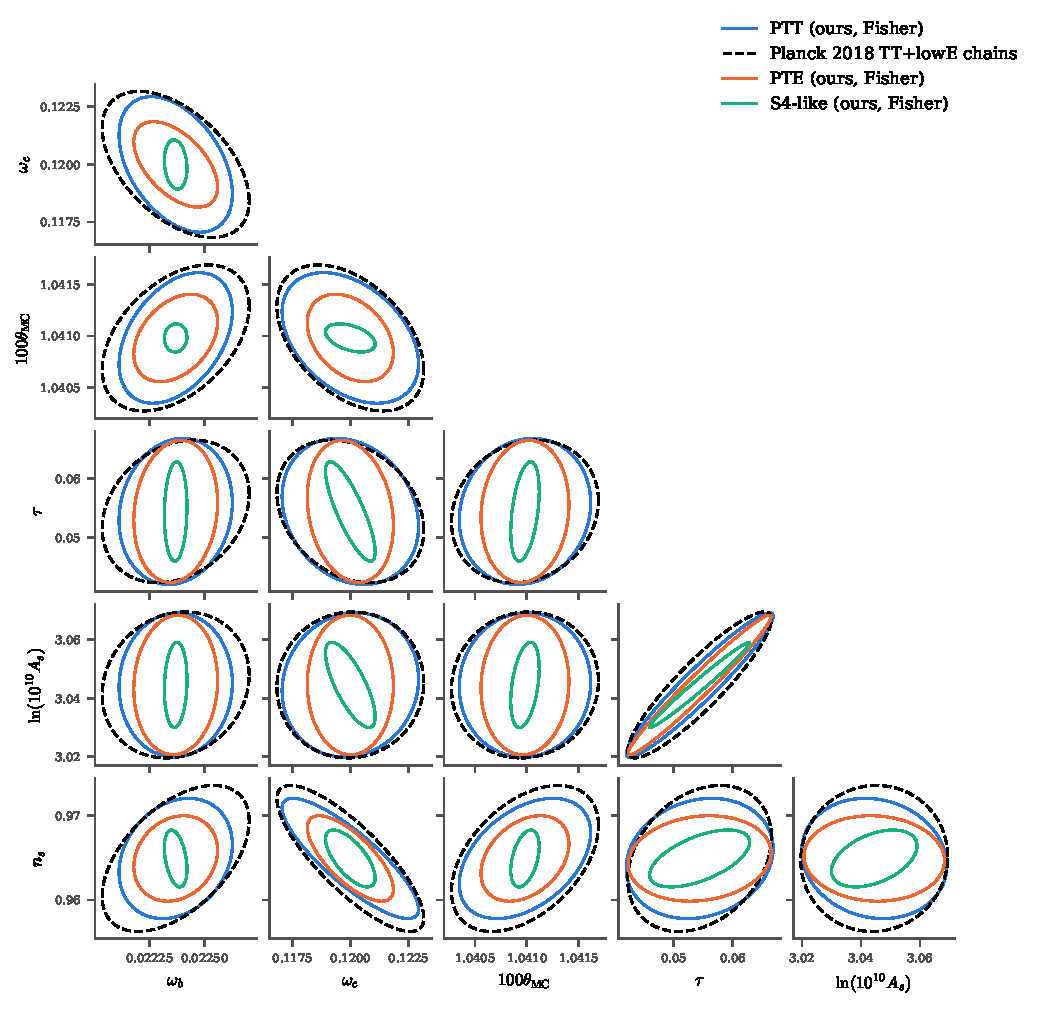
\includegraphics[width=0.92\linewidth]{figures/ch10/cmb_triangle.pdf}
\caption{Forecast against outcome. Each panel shows the $68\%$ ($\Delta\chi^2=2.30$) ellipse of a pair of $\Lambda$CDM
parameters, all others marginalised, centred on the fiducial model. Black dashed: the covariance of the official
Planck 2018 TT+lowE chains. Blue: our Fisher forecast for the same data. Orange: with polarization added. Green:
a futuristic ground survey. The forecast reproduces the sizes and orientations of the Planck ellipses; the
residual differences are in the parameters that share the high-$\ell$ damping tail with foregrounds.}
\label{10a:fig:cmb-triangle}
\end{figure}

\paragraph{Why the forecast is optimistic, and by how much.} The idealised experiment knows its noise exactly and
sees nothing but CMB. Planck's likelihood fits, in addition to the six cosmological parameters, some twenty
nuisance parameters: the amplitudes of the cosmic infrared background, of unresolved point sources and of the
Sunyaev--Zel'dovich effects in each frequency, Galactic dust residuals, and calibration factors (they are the
extra columns of the chain covariance file). Their spectra rise towards high $\ell$, where the damping tail of the
CMB measures $\omega_b$ and $n_s$, so marginalising over them costs precision exactly in the two parameters our
forecast overstates. The same mechanism explains the larger $\omega_b$--$n_s$ correlation in the real chains.

One nuisance can be added in a few lines, and it shows the mechanism at work. Planck compares the data with
$\Cell/y_P^2$, where the overall map calibration $y_P$ has a prior of $0.25\%$ \cite{Planck2018VI}. As a seventh
parameter with $\partial\Cell/\partial\ln y_P=-2\Cell$ and prior Fisher element $1/0.0025^2$, it is marginalised by inverting the
$7\times7$ matrix. The error on $10^9A_se^{-2\tau}$, which no other parameter can absorb, rises from $\TenFCmPttAsERel\%$ to
$\TenFCmCalAsERel\%$; Planck's TT+lowE value is $0.014/1.884=0.74\%$. The error on $\ln A_s$ goes from
$\TenFCmPttAsSharp$ to $\TenFCmCalAs$. One honest nuisance parameter turns a forecast that was a third too optimistic
for the best-measured amplitude into one that is within ten per cent of the published error.

\emph{Lesson.} The forecast was right about everything the idealised sky contains, the sizes and the
correlations, and wrong by about the amount that the missing nuisance parameters cost; adding even one of
them shows where the gap comes from.

\begin{figure}[htbp]
\centering
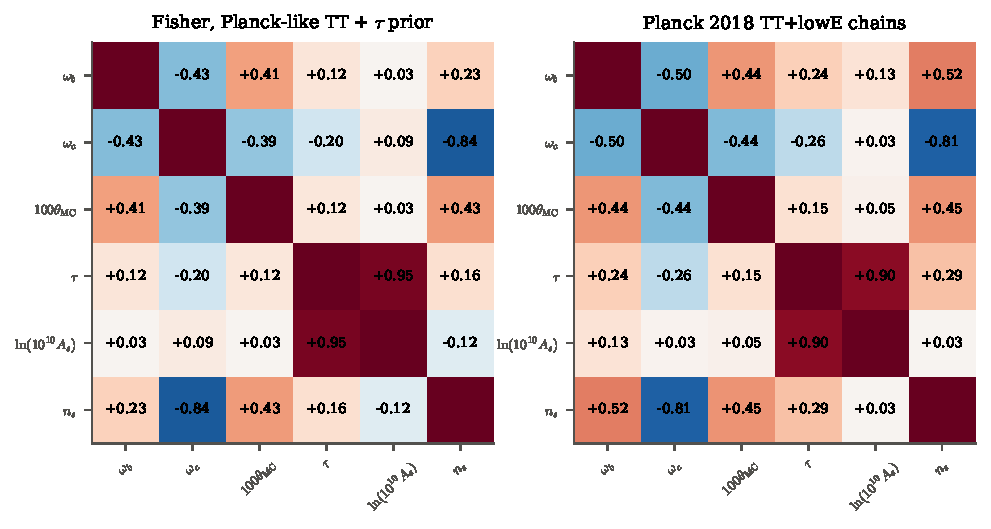
\includegraphics[width=0.98\linewidth]{figures/ch10/cmb_corr.pdf}
\caption{Correlation coefficients of the six parameters: our Fisher forecast for Planck-like temperature data with
a $\tau$ prior (left) and the covariance of the official Planck 2018 TT+lowE chains (right). The two strongest
correlations, $\tau$ with $\ln A_s$ and $\omega_c$ with $n_s$, are reproduced; the largest difference is
$\omega_b$ with $n_s$.}
\label{10a:fig:cmb-corr}
\end{figure}

\subsection{The classic degeneracies}
\label{10a:sec:cmb-degeneracies}

\paragraph{Amplitude and optical depth.} Free electrons after reionisation scatter CMB photons out of the line of
sight and suppress the anisotropy on all scales smaller than the horizon at reionisation by $e^{-2\tau}$, so for
$\ell\gtrsim10$ the temperature spectrum is proportional to $A_se^{-2\tau}$ (cosmology notes). \emph{Why this is a
degeneracy.} Write that as $\Cell\propto\exp(\ln A_s-2\tau)$. Then
\[
  \frac{\partial\Cell}{\partial\tau}=-2\Cell,\qquad \frac{\partial\Cell}{\partial\ln A_s}=\Cell :
\]
the two derivative vectors are parallel, both proportional to $\Cell$. In \eqref{10a:eq:cmb-fisher} every term of the
$(\tau,\ln A_s)$ block is then $\Cell^2$ times a product of the factors $-2$ and $1$, so the block is
\[
  f\begin{pmatrix}4&-2\\-2&1\end{pmatrix}=f\,\bm v\bm v\T,\qquad \bm v=\begin{pmatrix}-2\\1\end{pmatrix},\qquad
  f=\sum_\ell\frac{2\ell+1}2\fsky\Bigl(\frac{\Cell}{\Cell+N_\ell}\Bigr)^2 .
\]
Its determinant is $f^2(4-4)=0$: the matrix is singular, an exact degeneracy in the sense of \cref{10a:sec:two-faces}.
The unmeasured direction is the vector $\bm u$ with $\bm v\T\bm u=0$, $\bm u\propto(1,2)$: raising $\tau$ by $\delta$ and $\ln A_s$
by $2\delta$ leaves $\ln A_s-2\tau$, and so the spectrum, unchanged. This is the line $\ln A_s-2\tau=\text{const}$, of slope
$\dd\ln A_s/\dd\tau=2$. What the data do measure is the combination $y=\ln A_s-2\tau$, with variance $1/f$.

\emph{What the real Fisher matrix finds.} Our temperature-only Fisher matrix, \emph{without} the $\tau$ prior, finds
almost exactly this: the long axis of the $(\tau,\ln A_s)$ ellipse has slope $\dd\ln A_s/\dd\tau=\TenFCmSlopeAsTau$, the axes
differ by a factor $\TenFCmAxisRatio$, the marginalised errors are $\sigma_\tau=\TenFCmTauNoPrior$ and $\sigma_{\ln A_s}=\TenFCmAsNoPrior$,
yet the combination is measured to $\TenFCmAsENoPriorRel\%$. The slope is slightly below the exact null direction
$2$ because the lowest multipoles and the lensing of the spectrum (whose strength grows with $A_s$ but not with $\tau$)
carry a little information on each factor separately, which turns the singular block into a merely
ill-conditioned one.

\emph{Breaking it from outside.} The low-$\ell$ polarization measures $\tau$ on its own, with error $\sigma_\tau$; as a prior it
adds $1/\sigma_\tau^2$ to $F_{\tau\tau}$ (\cref{10a:sec:priors}). Now $\ln A_s=y+2\tau$, with $y$ fixed by the temperature data and
$\tau$ by the prior, two independent measurements, so
\[
  \Var(\ln A_s)=\Var y+4\,\sigma_\tau^2\approx4\,\sigma_\tau^2
\]
whenever the combination is measured much better than $2\sigma_\tau$. That is why the amplitude error in \cref{10a:tab:planck}
is set almost entirely by the $\tau$ prior: $\sigma_{\ln A_s}\approx2\sigma_\tau$.

\paragraph{The horizon-angle degeneracy: $\Omega_mh^3$.} The positions of the acoustic peaks fix the angle $\theta_*$ very
precisely, and the peak heights fix the physical matter density $\omega_m=\Omega_mh^2=\omega_b+\omega_c$ (the small neutrino
contribution neglected), where $h=H_0/(100\,\text{km\,s}^{-1}\,\text{Mpc}^{-1})$. The Hubble constant enters only
through the distance to last scattering, so changes of $h$ and $\Omega_m$ that keep $\theta_*$ fixed leave the spectrum
nearly unchanged; Percival et al.\ found that this degeneracy follows $\Omega_mh^{3.4}=\text{const}$ for the data of 2002
\cite{Percival2002}, and Planck quotes $\Omega_mh^3$ as the best-measured combination \cite{Planck2018VI}, eq.~(12). Our
forecast can find the exponent itself. \emph{The idea.} Among all the combinations $\Omega_mh^p$, the
best-measured one is the one with the smallest variance: the direction in the $(\ln\Omega_m,\ln h)$ plane along which
the data fix the parameters most tightly. So we write its variance as a function of $p$ and minimise. Since
$\Omega_m=\omega_m/h^2$, $\ln(\Omega_mh^p)=\ln\omega_m+(p-2)\ln h$, and its variance is
\begin{align}
  \Var\ln(\Omega_mh^p)
  &\eqby{1}\Var\ln\omega_m+2(p-2)\Cov(\ln\omega_m,\ln h)+(p-2)^2\Var\ln h,
  \nonumber\\
  p_{\rm best}&\eqby{2}2-\frac{\Cov(\ln\omega_m,\ln h)}{\Var\ln h},
  \label{10a:eq:pbest}
\end{align}
\begin{explain}
  \item $\Omega_mh^p=\omega_mh^{p-2}$; the variance of a sum.
  \item Set the derivative with respect to $p$ to zero.
\end{explain}
\emph{The ingredients.} Both $\ln\omega_m$ and $\ln h$ are derived parameters, so their variances and covariance come
from the delta method of \cref{10a:sec:reparam}, $\Cov(g,g')=\nabla g\T\Fish^{-1}\nabla g'$. The gradient of $\ln\omega_m$ is
$(1,1,0,0,0,0)/\omega_m$, nonzero only in $\omega_b$ and $\omega_c$. The gradient of $\ln h$ is $\nabla H_0/H_0$, because
$\ln h=\ln H_0-\ln100$ and $\dd\ln H_0=\dd H_0/H_0$; CAMB's background code gives
$\partial H_0/\partial(\omega_b,\omega_c,100\theta_{\rm MC})=(\TenFCmGradHzOb,\TenFCmGradHzOc,\TenFCmGradHzTh)$, the other three entries being zero.
The forecast gives
$p_{\rm best}=\TenFCmPttPbest$ for temperature and $\TenFCmPtePbest$ with polarization: Planck's $\Omega_mh^3$, derived here from a
Fisher matrix. With the much smaller errors of the futuristic survey it moves to $\TenFCmSfPbest$, which is the point
of Percival's different exponent: the best-measured combination depends on which multipoles carry the
information. The error on $\Omega_mh^3$ itself is $\TenFCmPttOmhThree$ ($\TenFCmPttOmhThreeRel\%$) against Planck's $0.00046$ for TT+lowE,
and $\TenFCmPteOmhThree$ against $0.00029$ with polarization.

\paragraph{Dark matter and tilt.} The strongest correlation not broken by an external prior is $\omega_c$ with $n_s$,
$\TenFCmRhoOcNsOurs$ in our forecast and $\TenFCmRhoOcNsPl$ in Planck's chains. More dark matter brings matter--radiation
equality earlier, which reduces the boost the first acoustic peaks receive from decaying potentials (cosmology
notes); the first peaks drop relative to the damping tail, which a slightly redder tilt (smaller $n_s$) also does.
\Cref{9c:sec:planck-ns} met the same correlation in the chain.

\subsection{A futuristic experiment, the reach in \texorpdfstring{$\ell$}{l} and the sky fraction}
\label{10a:sec:cmb-future}

A forecast is most useful for designing the next experiment. Take a ground-based survey with $1\,\mu$K\,arcmin in
temperature ($\sqrt2$ in polarization), a $1.4'$ beam, $\fsky=0.4$ and temperature and polarization at
$30\le\ell\le3000$ (the atmosphere prevents a ground telescope from measuring the largest scales), plus the same $\tau$
prior. Its errors are in the last column of \cref{10a:tab:planck}: $\omega_b$ improves by a factor $\TenFCmGainOb$ over the
Planck-like experiment, $\theta_{\rm MC}$ by $\TenFCmGainTh$, $\omega_c$ by $\TenFCmGainOc$, $n_s$ by $\TenFCmGainNs$, and even $\tau$ by
$\TenFCmGainTau$, although the survey sees no multipole below $30$. That last gain comes from lensing: the lensed
spectra we use depend on $A_s$ through the lensing strength but not on $\tau$, so a precise damping tail separates
the two factors. The same code with more parameters gives the larger forecasts of Jungman et al.\ and of Tegmark et al.\ (eleven parameters, \cite{TTH1997}, eqs.~(19)--(20)): each new parameter costs one more derivative of the spectra and one more row and column of $\Fish$. A real forecast at this noise level must include the non-Gaussian covariance that lensing
induces between multipoles, which reduces this gain (\cref{10a:sec:research}).

\emph{Which multipoles matter?} \Cref{10a:fig:cmb-lmax} recomputes the forecast for maximum multipoles from $500$ to
$3000$. For the Planck-like experiment, stopping at $\ell_{\max}=1000$ would multiply the error on $n_s$ by $\TenFCmLmThousandNs$
and on $\omega_b$ and $\theta_{\rm MC}$ by $\TenFCmLmThousandOb$, while $\tau$ and $\ln A_s$ barely care ($\TenFCmLmThousandTau$): the third
and higher peaks and the damping tail are where the densities and the tilt are measured.

\emph{How much sky?} Every term of \eqref{10a:eq:cmb-fisher} is proportional to $\fsky$, so the data part of $\Fish$ is too,
and every error that is not dominated by a prior scales as $\fsky^{-1/2}$. For the Planck-like experiment the error on
$n_s$ is $\TenFCmFskyLowNs$, $\TenFCmFskyMidNs$ and $\TenFCmFskyHighNs$ at $\fsky=\TenFCmFskyLowVal$, $\TenFCmFskyMidVal$ and $\TenFCmFskyHighVal$, and
$\TenFCmFskyMidNs\times\sqrt{\TenFCmFskyMidVal/\TenFCmFskyLowVal}\approx\TenFCmFskyLowNs$ and $\TenFCmFskyMidNs\times\sqrt{\TenFCmFskyMidVal/\TenFCmFskyHighVal}\approx\TenFCmFskyHighNs$; the error on $\tau$, held by its prior, moves only from
$\TenFCmFskyLowTau$ to $\TenFCmFskyHighTau$.

\begin{figure}[htbp]
\centering
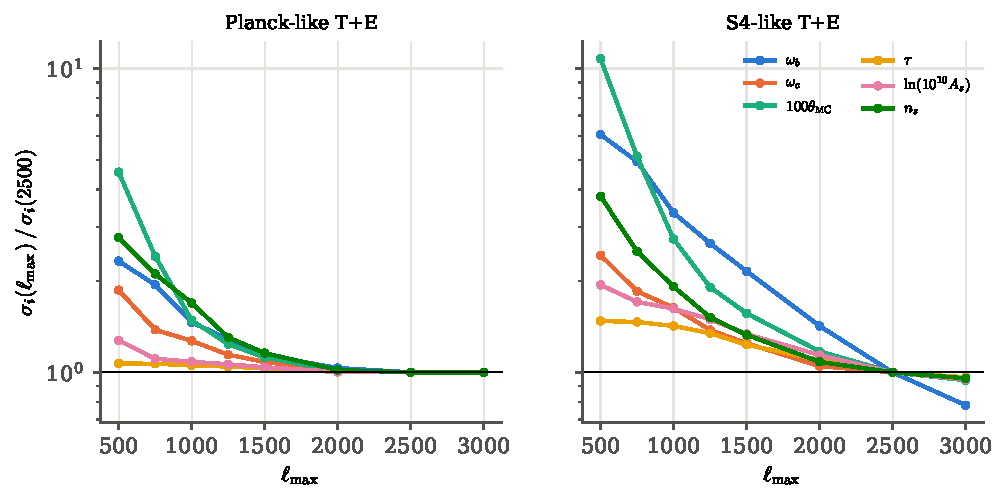
\includegraphics[width=0.98\linewidth]{figures/ch10/cmb_lmax.pdf}
\caption{How the forecast errors depend on the highest multipole used, relative to $\ell_{\max}=2500$. Left: the
Planck-like experiment (polarization stops at $\ell=2000$). Right: the futuristic survey. The densities, the angle and the
tilt keep improving into the damping tail; the amplitude and $\tau$ are fixed early by the $\tau$ prior.}
\label{10a:fig:cmb-lmax}
\end{figure}

\subsection{Is the forecast right? The chain and a thousand fits}
\label{10a:sec:cmb-check}

A forecast is a statement about an idealised analysis of idealised data. Two independent checks are possible
with tools the book already has: the Markov chain of \cref{ch:09}, which maps the actual posterior for one
simulated data set, and a Monte Carlo of maximum-likelihood fits, which measures the actual scatter over many.

\paragraph{The chain.} Run P6 of \cref{9c:sec:planck} sampled the six $\Lambda$CDM parameters from one simulated temperature
spectrum: one 143\,GHz-like channel ($7.22'$, $33\,\mu$K\,arcmin), $\fsky=0.57$, $2\le\ell\le2500$, the exact likelihood, and the
same $\tau$ prior. It sampled in a different basis, $\bm p=(\ln10^{10}A_s,n_s,H_0,\omega_b,\omega_c,\tau)$, with $H_0$ in place of
$\theta_{\rm MC}$. Our Fisher matrix for the same experiment is computed in the Planck basis and moved to the chain's basis
with the Jacobian rule \eqref{10a:eq:jacobian}. All entries of $\bm J=\partial\params/\partial\bm p$ are zeros and ones except the row of
$100\theta_{\rm MC}$, which depends on $H_0$, $\omega_b$ and $\omega_c$; CAMB's background code gives
$\partial(100\theta_{\rm MC})/\partial(H_0,\omega_b,\omega_c)=(\TenGFmDthHz,\TenGFmDthOb,\TenGFmDthOc)$. Then:

\begin{center}
\small
\renewcommand{\arraystretch}{1.15}
\begin{tabular}{@{}lcccccc@{}}
\toprule
 & $\ln(10^{10}A_s)$ & $n_s$ & $H_0$ & $\omega_b$ & $\omega_c$ & $\tau$\\\midrule
Fisher, $\bm J\T\Fish\bm J$ (CAMB derivatives) & $\TenGFmFAs$ & $\TenGFmFNs$ & $\TenGFmFHz$ & $\TenGFmFOb$ & $\TenGFmFOc$ & $\TenGFmFTau$\\
chain P6 (\cref{ch:09}) & $\TenGFmCAs$ & $\TenGFmCNs$ & $\TenGFmCHz$ & $\TenGFmCOb$ & $\TenGFmCOc$ & $\TenGFmCTau$\\
Fisher of \cref{ch:09} (emulator derivatives) & $\TenGFmNAs$ & $\TenGFmNNs$ & $\TenGFmNHz$ & $\TenGFmNOb$ & $\TenGFmNOc$ & $\TenGFmNTau$\\
$\TenGFmNsim$ maximum-likelihood fits & $\TenGFmMAs$ & $\TenGFmMNs$ & $\TenGFmMHz$ & $\TenGFmMOb$ & $\TenGFmMOc$ & $\TenGFmMTau$\\
\bottomrule
\end{tabular}
\end{center}

The Fisher errors agree with the widths of the chain to within one per cent for every parameter, and every
correlation coefficient agrees to within $\TenGFmMaxRhoDiff$; the strongest, $H_0$ with $\omega_c$, is $\TenGFmRhoHzOcF$ in both. Two
quite different computations stand behind this: our derivatives were taken in another basis by the four-point
rule and transformed with a Jacobian, chapter~9's came from an emulator of $\ln\Cell$, and the chain never used a
derivative at all.

\paragraph{A thousand fits.} The chain describes the posterior of one data set; the Cram\'er--Rao reading of $\Fish^{-1}$
is about the scatter of estimates over many. \pyname{07_fisher_vs_mcmc.py} draws $\TenGFmNsim$ new spectra and $\tau$
measurements from the same experiment and finds the maximum of the likelihood of each, a thousand
six-parameter maximisations. How should each be done?

\emph{One parameter first: a Newton step.} Near the current guess $\theta_n$ the score, the slope of $\ln\Like$, is
nearly a straight line in $\theta$, and its slope is minus the curvature: by \eqref{10a:eq:taylor},
$S(\theta)\approx S(\theta_n)-\mathcal H\,(\theta-\theta_n)$. The maximum is where the slope of the hill vanishes, $S=0$; solving the
straight line for that point gives $\theta=\theta_n+S(\theta_n)/\mathcal H$, slope over curvature. If $\ln\Like$ were an exact
parabola, one step would land on its top; for a nearly parabolic hill each step lands much closer.
\emph{Many parameters.} The same expansion of the score vector is $\bm S(\params)\approx\bm S(\params_n)-\bm{\mathcal H}(\params-\params_n)$, and
$\bm S=\bm0$ gives the step $\params_n+\bm{\mathcal H}^{-1}\bm S(\params_n)$. \emph{Replace the curvature by its average.} The observed
curvature $\bm{\mathcal H}$ of one noisy data set needs second derivatives of the model and, far from the peak, need not
be positive definite, in which case the step can go downhill. Its average over data, the Fisher matrix
\eqref{10a:eq:fisher-def}, is known in closed form, \eqref{10a:eq:cmb-fisher}, and is always positive definite, so the
step $\Fish^{-1}\bm S$ always has a positive component along the uphill direction: $\bm S\T\Fish^{-1}\bm S>0$ whenever
$\bm S\neq\bm0$. Near the peak the two curvatures differ only by the $1/\sqrt n$ fluctuation of
\cref{10a:sec:fisher-def}, so little speed is lost. This iteration is called \newterm{Fisher scoring}:
\begin{equation}
  \params\leftarrow\params+\Fish(\params)^{-1}\bm S(\params),
  \qquad
  S_i=\sum_\ell\frac{\nu_\ell}2\,\partial_i\Cell\,\frac{\Chat-\Cell-N_\ell}{(\Cell+N_\ell)^2},
  \quad\nu_\ell=(2\ell+1)\fsky,
  \label{10a:eq:scoring}
\end{equation}
with $\Fish(\params)$ \eqref{10a:eq:cmb-fisher} evaluated at the current point.

\emph{The score of the exact likelihood.} The score comes from the exact
$-2\ln\Like=\sum_\ell\nu_\ell[\Chat/(\Cell+N_\ell)+\ln(\Cell+N_\ell)]$ (\cref{9c:sec:cl-exact}). With $X_\ell=\Cell+N_\ell$, which depends on
$\theta_i$ only through $\Cell$,
\begin{align*}
  S_i=\partial_i\ln\Like
  &\eqby{1}-\frac12\sum_\ell\nu_\ell\Bigl[-\frac{\Chat}{X_\ell^2}+\frac1{X_\ell}\Bigr]\partial_i\Cell
   \eqby{2}\sum_\ell\frac{\nu_\ell}2\,\partial_i\Cell\,\frac{\Chat-X_\ell}{X_\ell^2},
  \\
  \E[S_i]&\eqby{3}\sum_\ell\frac{\nu_\ell}2\,\partial_i\Cell\,\frac{\E\Chat-X_\ell}{X_\ell^2}=0 .
\end{align*}
\begin{explain}
  \item $\ln\Like$ is $-\frac12$ of the sum; by the chain rule $\partial_i(1/X)=-\partial_i\Cell/X^2$ and $\partial_i\ln X=\partial_i\Cell/X$.
  \item Put the bracket over the common denominator $X_\ell^2$; this is the $S_i$ of \eqref{10a:eq:scoring}.
  \item The estimate is unbiased, $\E\Chat=\Cell+N_\ell=X_\ell$: the score has mean zero at the truth, as
        \eqref{10a:eq:score-mean} requires.
\end{explain}
The model spectrum is chapter~9's second-order emulator, so each step costs a fraction of a millisecond:
\pyfile[firstline=110,lastline=122,firstnumber=110]{code/ch10/07_fisher_vs_mcmc.py}{Fisher scoring: Newton's method with the expected curvature}
The median fit converges in $\TenGFmIter$ iterations. The scatter of the $\TenGFmNsim$ estimates is in the last row of the
table: between $\TenGFmMRAs$ and $\TenGFmMRNs$ times the Fisher errors, with a Monte Carlo uncertainty of $\pm\TenGFmErr\%$; the
mean offsets from the truth are a few hundredths of a standard deviation at most ($\TenGFmBiasAs$ for $\ln A_s$,
$\TenGFmBiasTau$ for $\tau$). The fraction of estimates inside the two-parameter $68.3\%$
ellipse of $(\ln A_s,n_s)$ is $\TenGFmInTwo$, and inside the six-dimensional $68.3\%$ ellipsoid ($\Delta\chi^2\le\TenGFmChiSix$) it is
$\TenGFmInSix$, against $0.683\pm\TenGFmBinErr$ (\cref{10a:fig:fisher-mcmc}). For this experiment maximum likelihood reaches the
Cram\'er--Rao bound and the posterior has the Fisher width. The ellipses enclose close to what they claim; both
fractions come out slightly low, by one to two Monte Carlo errors.

\begin{figure}[htbp]
\centering
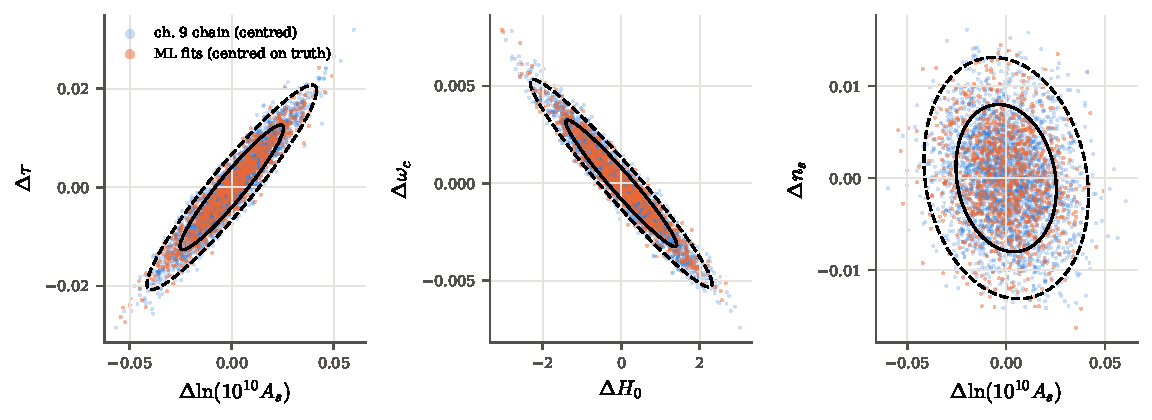
\includegraphics[width=0.98\linewidth]{figures/ch10/fisher_mcmc.pdf}
\caption{Three views of the same six-parameter problem in three planes: samples of the chapter-9 posterior for one
simulated sky (blue, centred on their mean), the maximum-likelihood estimates from $1000$ simulated skies
(orange, centred on the truth), and the Fisher ellipses ($\Delta\chi^2=2.30$, $6.18$) computed before any sky was
simulated.}
\label{10a:fig:fisher-mcmc}
\end{figure}

\paragraph{When the Fisher matrix fails.} Everything above worked because the CMB spectrum is nearly linear in the
parameters over a one-sigma region: the errors are tiny compared with the scale on which the spectrum bends.
Vallisneri lists what goes wrong when that is not true \cite{Vallisneri2008}, and the book has examples of each. At
low signal-to-noise the likelihood is not a parabola over the scatter of the estimates (Cowan's experiment with
$50$ events, \cref{10a:sec:cr-reach}; the skewed decay-time posterior of \cref{9c:sec:exp}). Near a physical boundary the
Gaussian approximation puts probability where the parameter cannot go (a tensor ratio or a neutrino mass near zero).
A quasi-singular Fisher matrix, with a direction the data barely constrain, makes $\Fish^{-1}$ meaningless in that
direction unless a prior is added. In all three cases the Fisher matrix is still the right first calculation, and
a chain on simulated data is the second.

\begin{inpractice}[Verification and research]
Here the Monte Carlo and the chain \emph{verified} a forecast that analytic theory already gave, as the
simulations of \cref{ch:08} verified the cosmic-variance formula. In research the roles reverse. Survey teams
produce Fisher forecasts for every design option because they are instantaneous, and then run full
chains on simulated data for the few designs that matter, because only the chain sees non-Gaussian
posteriors, physical boundaries, nuisance parameters with non-Gaussian priors and likelihoods that are not
Gaussian in the data. A forecast that survives that test is the one quoted in the proposal.
\end{inpractice}
\section{How it is done in research}
\label{10a:sec:research}

A survey team writing a proposal, or a collaboration choosing between two telescope designs, runs the same
calculation as \cref{10a:sec:cmb}, but every box of it is larger. A real forecast passes through those
boxes in a fixed order (\cref{10a:fig:research}); at each one the research version adds physics that the laptop
version replaced by something simpler, and each replacement has a measurable cost.

\begin{figure}[htbp]
\centering
\begin{tikzpicture}[
  bx/.style={draw=accent,thick,rounded corners=2pt,fill=ideabg,font=\small,
             minimum height=12mm,align=center,text width=37mm},
  lp/.style={draw=softgray,rounded corners=2pt,font=\footnotesize,align=center,text width=37mm,
             minimum height=9mm},
  flow/.style={->,thick,accent}]
  \node[bx] (s1) at (0,0)      {1. parameters, basis,\\ fiducial model};
  \node[bx] (s2) at (5.0,0)    {2. Boltzmann code:\\ $\Cell^{XY}$, $\Cell^{\phi\phi}$,\\ derivatives};
  \node[bx] (s3) at (10.0,0)   {3. instrument: beams,\\ noise, foregrounds,\\ $\fsky$};
  \node[bx] (s4) at (10.0,-2.6) {4. covariance of the\\ data: Gaussian\\ $+$ lensing};
  \node[bx] (s5) at (5.0,-2.6) {5. $\Fish$ per experiment;\\ add external data};
  \node[bx] (s6) at (0,-2.6)   {6. invert: errors,\\ ellipses, figures\\ of merit, design loop};
  \node[bx] (s7) at (0,-5.2)   {7. validate: chains on\\ mock data at the\\ fiducial};
  \draw[flow] (s1) -- (s2); \draw[flow] (s2) -- (s3); \draw[flow] (s3) -- (s4);
  \draw[flow] (s4) -- (s5); \draw[flow] (s5) -- (s6); \draw[flow] (s6) -- (s7);
  \node[lp] (l2) at (5.0,2.0)  {here: default CAMB,\\ 84 cached runs, step test};
  \node[lp] (l3) at (10.0,2.0) {here: white noise, one\\ nuisance (calibration)};
  \draw[softgray,dashed] (l2.south) -- (s2.north);
  \draw[softgray,dashed] (l3.south) -- (s3.north);
\end{tikzpicture}
\caption{The stages of a research CMB forecast (blue boxes, in order), with two of the simplifications
made by the laptop version (grey), each attached to the stage it simplifies.}
\label{10a:fig:research}
\end{figure}

\paragraph{1. Parameters, basis and fiducial.} The model is $\Lambda$CDM plus the extensions the survey targets (the
effective number of relativistic species $N_{\rm eff}$, which counts the light particles such as neutrinos that
behaved like radiation in the early universe and is about three in the standard model; the sum of neutrino masses;
the tensor ratio $r$), at a fiducial
point taken from the best current fit. The basis is chosen close to what the data measure ($\theta_{\rm MC}$ rather
than $H_0$, $\ln A_s$ at a pivot), so that the likelihood is nearly Gaussian in it and the finite differences behave;
the quantities people quote ($H_0$; $\sigma_8$, the root-mean-square matter fluctuation in spheres of $8\,h^{-1}$\,Mpc;
$\Omega_mh^3$) are derived afterwards with the Jacobian or delta-method rule
(\cref{10a:sec:reparam}). \emph{Here:} the six-parameter Planck basis at the Planck 2018 best fit.

\paragraph{2. Theory and derivatives.} A Boltzmann code such as CAMB is run at raised accuracy settings and to
higher multipoles than the survey will use, producing lensed $TT$, $TE$, $EE$, $BB$ spectra and the spectrum of the
lensing potential $\Cell^{\phi\phi}$ (the projected gravitational potential that deflects CMB photons on their way to us).
Derivatives are taken by finite differences and checked as in \cref{10a:sec:numderiv}:
steps halved and doubled, two- and four-point rules compared, and the code's accuracy raised until the forecast stops
moving. \emph{Here:} default accuracy, $\ell\le3000$, $84$ cached runs; the step test moved no error by more than a tenth of
a per cent. The cost is nothing for a Planck-like experiment and possibly a few per cent for a survey that uses
$\ell>3000$.

\paragraph{3. The instrument.} For each frequency channel: beam; white-noise depth; for a ground telescope the ``$1/f$''
noise, slow drifts of the atmospheric emission and of the detector gain whose power rises at low frequencies and
therefore adds noise at low $\ell$; the hit map, how many times each patch of sky was observed, which sets the noise
of each pixel; and the sky mask. Foregrounds (Galactic dust and synchrotron, the cosmic infrared background,
Sunyaev--Zel'dovich effects, point sources) are removed by a simulated component separation, which uses the several
frequencies to subtract emission whose dependence on frequency differs from that of the CMB; what is left after it is
added to the noise as a residual power spectrum. Lensing reconstruction, the estimate of the deflection field from
the distortions it leaves in the small-scale CMB, has a noise of its own, a noise spectrum that plays for
$\Cell^{\phi\phi}$ the part $N_\ell$ plays for $\Cell$. \emph{Here:} white noise, combined by inverse variance, no foregrounds, and a single
nuisance parameter. The cost was measured in \cref{10a:sec:cmb-planck}: errors on $\omega_b$ and $n_s$ about twenty per cent too
small for Planck, most of the gap on $A_se^{-2\tau}$ closed by the calibration nuisance alone.

\paragraph{4. The covariance of the data.} The Gaussian, $\fsky$-scaled covariance \eqref{10a:eq:cmb-fisher-TE} is the starting
point. Research forecasts add the covariance that lensing induces between multipoles of the lensed spectra and
between them and $\Cell^{\phi\phi}$: all modes are deflected by the same large-scale field, so a fluctuation of that field
moves power at many multipoles together and correlates them, which is why lensing is a non-Gaussian, mode-coupling
operation. For small or irregular sky patches they add the mode coupling of the mask (cutting the sky mixes
neighbouring multipoles, \cref{ch:08}), estimated with simulations. \emph{Here:} Gaussian covariance with
$(2\ell+1)\fsky$ modes. The cost is small for Planck-like noise and large for the futuristic survey, whose $\tau$
improvement of \cref{10a:sec:cmb-future} comes from lensing information this approximation overstates.

\paragraph{5. Fisher matrices and external data.} One matrix per experiment and per data product, in a common
parameter basis (Jacobians where the bases differ), added together: the CMB, a $\tau$ measurement from large-scale
polarization, baryon acoustic oscillations, supernovae (\cref{10a:sec:priors}). Overlapping sky areas are not
independent and must not simply be added; the overlap is treated as one experiment with a joint covariance.
\emph{Here:} one CMB matrix plus a $\tau$ prior.

\paragraph{6. Reading and design.} Marginalised errors, triangle plots of ellipses, figures of merit, and the
same numbers recomputed as the design changes (noise level, beam, sky fraction, observing time): a forecast is
usually a curve or a grid, not a number, as in \cref{10a:fig:cmb-lmax}. One more product is routine: the shift of
the parameters that a small unmodelled systematic $\delta\bm\mu$ in the data would cause. \emph{The question.} If the data
have mean $\bm\mu(\params_0)+\delta\bm\mu$ instead of $\bm\mu(\params_0)$, where does the fit land on average? The fit lands
where the score vanishes, so we ask where the \emph{average} score vanishes. Name the vector $\bm b$ with components
$b_i=\bm\mu_{,i}\T\Cmat^{-1}\delta\bm\mu$, the overlap of the systematic with the response of the data to $\theta_i$; this is
what $\bigl[\bm\mu_{,i}\T\Cmat^{-1}\delta\bm\mu\bigr]_i$ below denotes. Then, for Gaussian data,
\begin{align}
  \E\bigl[S_i(\params_0)\bigr]
  &\eqby{1}\bm\mu_{,i}\T\Cmat^{-1}\E[\bm r]
   +\tfrac12\bigl(\E[\bm r\T\Cmat^{-1}\Cmat_{,i}\Cmat^{-1}\bm r]-\Tr\Cmat^{-1}\Cmat_{,i}\bigr)
   \eqby{2}\bm\mu_{,i}\T\Cmat^{-1}\delta\bm\mu=b_i ,
  \nonumber\\
  \E\bigl[S_i(\params_0+\delta\params)\bigr]
  &\eqby{3}b_i+\sum_j\delta\theta_j\,\E\bigl[\partial_jS_i\bigr]
   \eqby{4}b_i-\sum_jF_{ij}\,\delta\theta_j ,
  \nonumber\\
  \bm0=\bm b-\Fish\,\delta\params
  &\eqby{5}\quad\Rightarrow\quad
  \delta\params=\Fish^{-1}\bigl[\bm\mu_{,i}\T\Cmat^{-1}\delta\bm\mu\bigr]_i ,
  \label{10a:eq:fisher-bias}
\end{align}
\begin{explain}
  \item The score \eqref{10a:eq:gauss-S}, with residual $\bm r=\data-\bm\mu(\params_0)$, averaged term by term.
  \item The residual is now $\bm r=\delta\bm\mu+\bm n$ with noise $\bm n$ of mean zero and covariance $\Cmat$, so $\E\bm r=\delta\bm\mu$. In the
        second term, $\E[\bm r\T\bm M\bm r]=\Tr(\bm M\Cmat)+\delta\bm\mu\T\bm M\delta\bm\mu$; the trace equals $\Tr\Cmat^{-1}\Cmat_{,i}$ and cancels, and
        the rest is second order in $\delta\bm\mu$, which we drop.
  \item Expand the average score to first order in the shift $\delta\params$.
  \item The average derivative of the score is the average second derivative of $\ln\Like$, which is $-F_{ij}$ by
        \eqref{10a:eq:fisher-def} (to zeroth order in $\delta\bm\mu$).
  \item Set the average score to zero and solve for $\delta\params$.
\end{explain}
This is the bias a systematic produces, in units that can be compared with $\Fish^{-1}$ directly. \emph{A check
with one parameter.} Let the data be a template of known shape with amplitude $A$, $\bm\mu=A\bm s$, so $\bm\mu_{,A}=\bm s$
and $F_{AA}=\bm s\T\Cmat^{-1}\bm s$ (\cref{10a:sec:gauss-ex}), and let the systematic be a calibration error that scales the
whole signal, $\delta\bm\mu=\epsilon\bm\mu=\epsilon A\bm s$. Then $b_A=\epsilon A\,\bm s\T\Cmat^{-1}\bm s=\epsilon A\,F_{AA}$ and $\delta A=b_A/F_{AA}=\epsilon A$: a calibration
off by $1\%$ moves the amplitude by $1\%$, as it must. Requirements on calibration, beam knowledge and foreground
residuals are set with this formula: the systematic is acceptable if $\delta\params$ is small against the errors.

\paragraph{7. Validation.} For the designs that matter, mock data are generated at the fiducial model and run
through the full likelihood with a sampler (for example Cobaya, a Markov chain code of the kind built in
\cref{ch:09}), and the posterior is compared with
the Fisher ellipses. This is where non-Gaussian posteriors, physical boundaries (a neutrino mass near zero, a
tensor ratio near zero) and priors that are not Gaussian are found. \emph{Here:} the chain of \cref{ch:09} with an emulated
spectrum and $1000$ maximum-likelihood fits by Fisher scoring, which agreed with the forecast to one or two per cent.
For the full problem the chains take cluster hours per design; ours took seconds, because the model was an emulator
and the likelihood had no nuisance parameters.

\begin{table}[htbp]
\centering
\small
\renewcommand{\arraystretch}{1.2}
\begin{tabular}{@{}p{0.17\linewidth}p{0.27\linewidth}p{0.24\linewidth}p{0.25\linewidth}@{}}
\toprule
stage & research version & laptop version (here) & what the reduction costs\\\midrule
theory & high-accuracy Boltzmann runs to $\ell\sim5000$ & default CAMB, $\ell\le3000$, $84$ cached runs & $<0.1\%$ on the errors (step test); more for $\ell>3000$\\
noise & per-channel, anisotropic, $1/f$, foreground residuals & white, inverse-variance combined & $\omega_b$, $n_s$ errors $\sim20\%$ too small vs Planck\\
nuisances & $\sim20$ foreground and calibration parameters & calibration only (as a demonstration) & residual optimism in damping-tail parameters\\
sky & mask with mode coupling, simulated covariance & $(2\ell+1)\fsky$ modes & a few per cent at $\fsky\gtrsim0.4$; worse at low $\ell$\\
lensing & lensing reconstruction, lensing-induced covariance & lensed spectra, Gaussian covariance & futuristic $\tau$, $A_s$ gains overstated\\
low $\ell$ & non-Gaussian low-$\ell$ likelihood & Gaussian $\tau$ prior $0.0086$ & no skewness of $\tau$ near zero\\
validation & full-likelihood chains on mock data & chain of \cref{ch:09} (emulator), $1000$ fits & none here; decisive with real complexity\\
\bottomrule
\end{tabular}
\caption{Each reduction made in the laptop version, what the research analysis does instead, and what the reduction costs.}
\label{10a:tab:laptop}
\end{table}

\paragraph{How far a forecast is from reality.} \Cref{10a:fig:ratio} condenses the comparison with Planck into one
picture: the ratio of our forecast errors to the published ones. It is the realistic expectation for a forecast
built as above: right in the parameters set by a prior or by the peak positions, optimistic by up to a
quarter where unmodelled nuisances live. A research forecast closes most of the remaining gap by adding stages 3
and 4 in full.

\begin{figure}[htbp]
\centering
\begin{tikzpicture}
\begin{axis}[
  width=0.82\linewidth, height=5.2cm,
  ybar, bar width=7pt, ymin=0.5, ymax=1.15,
  symbolic x coords={wb,wc,th,tau,lnA,ns},
  xtick=data,
  xticklabels={$\omega_b$,$\omega_c$,$100\theta_{\rm MC}$,$\tau$,$\ln(10^{10}A_s)$,$n_s$},
  ylabel={$\sigma_{\rm forecast}/\sigma_{\rm Planck\,2018}$},
  legend style={at={(0.5,1.03)},anchor=south,font=\footnotesize,draw=none,fill=none,legend columns=2},
  legend cell align=left,
  extra y ticks={1}, extra y tick style={grid=major,grid style={black,thin}},
  tick label style={font=\footnotesize}, label style={font=\small}]
  \addplot[fill=formblue!70,draw=formblue] coordinates
    {(wb,\TenFCmRatTTOb) (wc,\TenFCmRatTTOc) (th,\TenFCmRatTTTh) (tau,\TenFCmRatTTTau) (lnA,\TenFCmRatTTAs) (ns,\TenFCmRatTTNs)};
  \addplot[fill=fibreorange!70,draw=fibreorange] coordinates
    {(wb,\TenFCmRatTEOb) (wc,\TenFCmRatTEOc) (th,\TenFCmRatTETh) (tau,\TenFCmRatTETau) (lnA,\TenFCmRatTEAs) (ns,\TenFCmRatTENs)};
  \legend{{TT\,+\,lowE},{TT,TE,EE\,+\,lowE}}
\end{axis}
\end{tikzpicture}
\caption{Our Fisher forecast errors divided by the published Planck 2018 errors for the same data combinations. A
bar at one is a perfect forecast. The amplitude and $\tau$ are held by the $\tau$ prior and come out right; the
densities, the angle and above all $\omega_b$ and $n_s$, which share the damping tail with foregrounds, come out too
small, because the idealised experiment has no foreground nuisances to marginalise.}
\label{10a:fig:ratio}
\end{figure}

\begin{recap}
\begin{itemize}
  \item The Fisher matrix $F_{ij}=-\E[\partial_i\partial_j\ln\Like]=\E[S_iS_j]$, at a fiducial model, is the average curvature of the
        log-likelihood and the covariance of the score; it needs a model of the experiment, not data.
  \item Cram\'er--Rao: $\Cov\hat\params-\Fish^{-1}$ is positive semidefinite for every unbiased estimator; maximum likelihood reaches
        the bound for linear-Gaussian models and for informative data (Cowan's experiment from $\sim500$ events on).
  \item Gaussian data: $F_{ij}=\bm\mu_{,i}\T\Cmat^{-1}\bm\mu_{,j}+\frac12\Tr[\Cmat^{-1}\Cmat_{,i}\Cmat^{-1}\Cmat_{,j}]$, first derivatives only; the CMB is the
        covariance channel, $F_{ij}=\sum_\ell\frac{(2\ell+1)\fsky}2\partial_i\Cell\partial_j\Cell/(\Cell+N_\ell)^2$.
  \item Marginalised error $\sqrt{(\Fish^{-1})_{ii}}$ (invert, then read) versus conditional $1/\sqrt{F_{ii}}$; the difference is a Schur
        complement. Two-parameter ellipses at $\Delta\chi^2=2.30,\,6.18$ hold $68.3\%$, $95.4\%$.
  \item Priors and independent experiments add as matrices; a change of parameters is $\bm J\T\Fish\bm J$; derived quantities use
        $\nabla g\T\Fish^{-1}\nabla g$; nuisances are marginalised by inverting.
  \item Finite-difference steps of a fraction of the expected error, checked by halving and doubling; noisy derivatives make
        forecasts too optimistic.
  \item Reproduced: Cowan's two-parameter errors; Knox 1995's tilt and pivot amplitude errors and pivot $\ell_*=210$; Planck 2018
        errors within $\sim25\%$ (better with a calibration nuisance); $\Omega_mh^3$ and $A_se^{-2\tau}$ as the degeneracy directions;
        the chapter-9 chain and $1000$ maximum-likelihood fits within one or two per cent.
\end{itemize}
\end{recap}
\providecommand{\TenBdetRho}{}\renewcommand{\TenBdetRho}{5}
\providecommand{\TenBdetT}{}\renewcommand{\TenBdetT}{16}
\providecommand{\TenBdetfs}{}\renewcommand{\TenBdetfs}{1024}
\providecommand{\TenBdetfhi}{}\renewcommand{\TenBdetfhi}{219.9}
\providecommand{\TenBdetDur}{}\renewcommand{\TenBdetDur}{5.959}
\providecommand{\TenBdetStrainRatio}{}\renewcommand{\TenBdetStrainRatio}{5.314}
\providecommand{\TenBdetZzeroMean}{}\renewcommand{\TenBdetZzeroMean}{-7.002\times10^{-4}}
\providecommand{\TenBdetZzeroSd}{}\renewcommand{\TenBdetZzeroSd}{0.9939}
\providecommand{\TenBdetZoneMean}{}\renewcommand{\TenBdetZoneMean}{5.001}
\providecommand{\TenBdetZoneSd}{}\renewcommand{\TenBdetZoneSd}{0.9945}
\providecommand{\TenBdetMzeroMed}{}\renewcommand{\TenBdetMzeroMed}{4.226}
\providecommand{\TenBdetMoneMed}{}\renewcommand{\TenBdetMoneMed}{5.214}
\providecommand{\TenBdetThrZ}{}\renewcommand{\TenBdetThrZ}{2.326}
\providecommand{\TenBdetThrM}{}\renewcommand{\TenBdetThrM}{5.123}
\providecommand{\TenBdetPdZ}{}\renewcommand{\TenBdetPdZ}{0.9965}
\providecommand{\TenBdetPdZth}{}\renewcommand{\TenBdetPdZth}{0.9962}
\providecommand{\TenBdetPdM}{}\renewcommand{\TenBdetPdM}{0.54}
\providecommand{\TenBdetNlags}{}\renewcommand{\TenBdetNlags}{16384}
\providecommand{\TenBdetNeff}{}\renewcommand{\TenBdetNeff}{5000}
\providecommand{\TenBsdGTwo}{}\renewcommand{\TenBsdGTwo}{2.367}
\providecommand{\TenBsdTTwo}{}\renewcommand{\TenBsdTTwo}{1.226}
\providecommand{\TenBcovGTwo}{}\renewcommand{\TenBcovGTwo}{27.2}
\providecommand{\TenBcovTTwo}{}\renewcommand{\TenBcovTTwo}{58.65}
\providecommand{\TenBwidGTwo}{}\renewcommand{\TenBwidGTwo}{0.709}
\providecommand{\TenBwidTTwo}{}\renewcommand{\TenBwidTTwo}{1.001}
\providecommand{\TenBsdGFour}{}\renewcommand{\TenBsdGFour}{1.253}
\providecommand{\TenBsdTFour}{}\renewcommand{\TenBsdTFour}{1.122}
\providecommand{\TenBcovGFour}{}\renewcommand{\TenBcovGFour}{49.95}
\providecommand{\TenBcovTFour}{}\renewcommand{\TenBcovTFour}{62.25}
\providecommand{\TenBwidGFour}{}\renewcommand{\TenBwidGFour}{0.8662}
\providecommand{\TenBwidTFour}{}\renewcommand{\TenBwidTFour}{1.001}
\providecommand{\TenBsdGEight}{}\renewcommand{\TenBsdGEight}{1.087}
\providecommand{\TenBsdTEight}{}\renewcommand{\TenBsdTEight}{1.065}
\providecommand{\TenBcovGEight}{}\renewcommand{\TenBcovGEight}{60.3}
\providecommand{\TenBcovTEight}{}\renewcommand{\TenBcovTEight}{64.8}
\providecommand{\TenBwidGEight}{}\renewcommand{\TenBwidGEight}{0.9356}
\providecommand{\TenBwidTEight}{}\renewcommand{\TenBwidTEight}{1.001}
\providecommand{\TenBsdGSixteen}{}\renewcommand{\TenBsdGSixteen}{1.043}
\providecommand{\TenBsdTSixteen}{}\renewcommand{\TenBsdTSixteen}{1.036}
\providecommand{\TenBcovGSixteen}{}\renewcommand{\TenBcovGSixteen}{64.4}
\providecommand{\TenBcovTSixteen}{}\renewcommand{\TenBcovTSixteen}{66.4}
\providecommand{\TenBwidGSixteen}{}\renewcommand{\TenBwidGSixteen}{0.9682}
\providecommand{\TenBwidTSixteen}{}\renewcommand{\TenBwidTSixteen}{1.001}
\providecommand{\TenBsdGThirtyTwo}{}\renewcommand{\TenBsdGThirtyTwo}{1.028}
\providecommand{\TenBsdTThirtyTwo}{}\renewcommand{\TenBsdTThirtyTwo}{1.026}
\providecommand{\TenBcovGThirtyTwo}{}\renewcommand{\TenBcovGThirtyTwo}{66.4}
\providecommand{\TenBcovTThirtyTwo}{}\renewcommand{\TenBcovTThirtyTwo}{67.35}
\providecommand{\TenBwidGThirtyTwo}{}\renewcommand{\TenBwidGThirtyTwo}{0.9843}
\providecommand{\TenBwidTThirtyTwo}{}\renewcommand{\TenBwidTThirtyTwo}{1.001}
\providecommand{\TenBcovMCerr}{}\renewcommand{\TenBcovMCerr}{1.043}
\providecommand{\TenBcfPhicA}{}\renewcommand{\TenBcfPhicA}{1.306}
\providecommand{\TenBcfTcA}{}\renewcommand{\TenBcfTcA}{0.7212}
\providecommand{\TenBcfMcA}{}\renewcommand{\TenBcfMcA}{0.003859}
\providecommand{\TenBcfMuA}{}\renewcommand{\TenBcfMuA}{0.3951}
\providecommand{\TenBcfCorrA}{}\renewcommand{\TenBcfCorrA}{0.899}
\providecommand{\TenBcfPhicB}{}\renewcommand{\TenBcfPhicB}{1.282}
\providecommand{\TenBcfTcB}{}\renewcommand{\TenBcfTcB}{0.7128}
\providecommand{\TenBcfMcB}{}\renewcommand{\TenBcfMcB}{0.004}
\providecommand{\TenBcfMuB}{}\renewcommand{\TenBcfMuB}{0.4083}
\providecommand{\TenBcfCorrB}{}\renewcommand{\TenBcfCorrB}{0.906}
\providecommand{\TenBcfPhicC}{}\renewcommand{\TenBcfPhicC}{1.635}
\providecommand{\TenBcfTcC}{}\renewcommand{\TenBcfTcC}{1.013}
\providecommand{\TenBcfMcC}{}\renewcommand{\TenBcfMcC}{0.02036}
\providecommand{\TenBcfMuC}{}\renewcommand{\TenBcfMuC}{0.5434}
\providecommand{\TenBcfCorrC}{}\renewcommand{\TenBcfCorrC}{0.927}
\providecommand{\TenBcfPhicD}{}\renewcommand{\TenBcfPhicD}{2.019}
\providecommand{\TenBcfTcD}{}\renewcommand{\TenBcfTcD}{1.441}
\providecommand{\TenBcfMcD}{}\renewcommand{\TenBcfMcD}{0.1137}
\providecommand{\TenBcfMuD}{}\renewcommand{\TenBcfMuD}{1.519}
\providecommand{\TenBcfCorrD}{}\renewcommand{\TenBcfCorrD}{0.9545}
\providecommand{\TenBcfPhicE}{}\renewcommand{\TenBcfPhicE}{1.986}
\providecommand{\TenBcfTcE}{}\renewcommand{\TenBcfTcE}{1.43}
\providecommand{\TenBcfMcE}{}\renewcommand{\TenBcfMcE}{0.1566}
\providecommand{\TenBcfMuE}{}\renewcommand{\TenBcfMuE}{1.944}
\providecommand{\TenBcfCorrE}{}\renewcommand{\TenBcfCorrE}{0.9583}
\providecommand{\TenBcfMaxDev}{}\renewcommand{\TenBcfMaxDev}{2.33}
\providecommand{\TenBcfFbar}{}\renewcommand{\TenBcfFbar}{64.26}
\providecommand{\TenBcfFrms}{}\renewcommand{\TenBcfFrms}{44.14}
\providecommand{\TenBcfTcAlone}{}\renewcommand{\TenBcfTcAlone}{0.2041}
\providecommand{\TenBcfTcPhic}{}\renewcommand{\TenBcfTcPhic}{0.3605}
\providecommand{\TenBcfFpeak}{}\renewcommand{\TenBcfFpeak}{55.35}
\providecommand{\TenBcfTcPhicFisher}{}\renewcommand{\TenBcfTcPhicFisher}{0.3605}
\providecommand{\TenBenvMc}{}\renewcommand{\TenBenvMc}{19.39}
\providecommand{\TenBenvflo}{}\renewcommand{\TenBenvflo}{19.96}
\providecommand{\TenBenvfhi}{}\renewcommand{\TenBenvfhi}{1}
\providecommand{\TenBenvfisco}{}\renewcommand{\TenBenvfisco}{4.391}
\providecommand{\TenBenvEpsDfA}{}\renewcommand{\TenBenvEpsDfA}{0.6913}
\providecommand{\TenBenvDpsiDfA}{}\renewcommand{\TenBenvDpsiDfA}{2.021\times10^{6}}
\providecommand{\TenBenvBDfA}{}\renewcommand{\TenBenvBDfA}{-3.778}
\providecommand{\TenBenvEpsDfB}{}\renewcommand{\TenBenvEpsDfB}{0.01549}
\providecommand{\TenBenvDpsiDfB}{}\renewcommand{\TenBenvDpsiDfB}{35351}
\providecommand{\TenBenvBDfB}{}\renewcommand{\TenBenvBDfB}{-4.333}
\providecommand{\TenBenvEpsAcc}{}\renewcommand{\TenBenvEpsAcc}{0.006635}
\providecommand{\TenBenvDpsiAcc}{}\renewcommand{\TenBenvDpsiAcc}{27371}
\providecommand{\TenBenvBAcc}{}\renewcommand{\TenBenvBAcc}{-3.111}
\providecommand{\TenBenvEpsPull}{}\renewcommand{\TenBenvEpsPull}{4.911\times10^{-6}}
\providecommand{\TenBenvDpsiPull}{}\renewcommand{\TenBenvDpsiPull}{39.45}
\providecommand{\TenBenvBPull}{}\renewcommand{\TenBenvBPull}{-2.111}
\providecommand{\TenBenvEpsEdd}{}\renewcommand{\TenBenvEpsEdd}{5.926\times10^{-7}}
\providecommand{\TenBenvDpsiEdd}{}\renewcommand{\TenBenvDpsiEdd}{1.353}
\providecommand{\TenBenvBEdd}{}\renewcommand{\TenBenvBEdd}{-4.333}
\providecommand{\TenBenvEpsMig}{}\renewcommand{\TenBenvEpsMig}{0.03892}
\providecommand{\TenBenvDpsiMig}{}\renewcommand{\TenBenvDpsiMig}{1.027\times10^{5}}
\providecommand{\TenBenvBMig}{}\renewcommand{\TenBenvBMig}{-4}
\providecommand{\TenBenvfeq}{}\renewcommand{\TenBenvfeq}{16.75}
\providecommand{\TenBenvClosedErr}{}\renewcommand{\TenBenvClosedErr}{2.285\times10^{-6}}
\providecommand{\TenBrobFstar}{}\renewcommand{\TenBrobFstar}{19.09}
\providecommand{\TenBrobReadA}{}\renewcommand{\TenBrobReadA}{4.642\times10^{-17}}
\providecommand{\TenBrobOursA}{}\renewcommand{\TenBrobOursA}{4.628\times10^{-17}}
\providecommand{\TenBrobReadB}{}\renewcommand{\TenBrobReadB}{2.537\times10^{-18}}
\providecommand{\TenBrobOursB}{}\renewcommand{\TenBrobOursB}{2.544\times10^{-18}}
\providecommand{\TenBrobReadC}{}\renewcommand{\TenBrobReadC}{2.894\times10^{-19}}
\providecommand{\TenBrobOursC}{}\renewcommand{\TenBrobOursC}{2.880\times10^{-19}}
\providecommand{\TenBrobReadD}{}\renewcommand{\TenBrobReadD}{4.308\times10^{-20}}
\providecommand{\TenBrobOursD}{}\renewcommand{\TenBrobOursD}{4.313\times10^{-20}}
\providecommand{\TenBrobReadE}{}\renewcommand{\TenBrobReadE}{1.173\times10^{-20}}
\providecommand{\TenBrobOursE}{}\renewcommand{\TenBrobOursE}{1.201\times10^{-20}}
\providecommand{\TenBrobReadF}{}\renewcommand{\TenBrobReadF}{1.716\times10^{-20}}
\providecommand{\TenBrobOursF}{}\renewcommand{\TenBrobOursF}{1.737\times10^{-20}}
\providecommand{\TenBrobReadG}{}\renewcommand{\TenBrobReadG}{4.019\times10^{-20}}
\providecommand{\TenBrobOursG}{}\renewcommand{\TenBrobOursG}{4.615\times10^{-20}}
\providecommand{\TenBrobRatioMin}{}\renewcommand{\TenBrobRatioMin}{0.9953}
\providecommand{\TenBrobRatioMax}{}\renewcommand{\TenBrobRatioMax}{1.148}
\providecommand{\TenBrobDevLow}{}\renewcommand{\TenBrobDevLow}{8.594}
\providecommand{\TenBrobASDmin}{}\renewcommand{\TenBrobASDmin}{1.178\times10^{-20}}
\providecommand{\TenBrobfmin}{}\renewcommand{\TenBrobfmin}{7.256}
\providecommand{\TenBrobJhGB}{}\renewcommand{\TenBrobJhGB}{3.107\times10^{-18}}
\providecommand{\TenBrobJsnr}{}\renewcommand{\TenBrobJsnr}{139.8}
\providecommand{\TenBrobJsnrNoConf}{}\renewcommand{\TenBrobJsnrNoConf}{147.6}
\providecommand{\TenBrobGWfFive}{}\renewcommand{\TenBrobGWfFive}{15.83}
\providecommand{\TenBrobGWfOne}{}\renewcommand{\TenBrobGWfOne}{28.94}
\providecommand{\TenBrobBigf}{}\renewcommand{\TenBrobBigf}{2.927\times10^{-5}}
\providecommand{\TenBrobTtwoDiff}{}\renewcommand{\TenBrobTtwoDiff}{4.441\times10^{-16}}
\providecommand{\TenBppSNR}{}\renewcommand{\TenBppSNR}{13.25}
\providecommand{\TenBppMc}{}\renewcommand{\TenBppMc}{19.39}
\providecommand{\TenBppEta}{}\renewcommand{\TenBppEta}{0.001396}
\providecommand{\TenBppflo}{}\renewcommand{\TenBppflo}{19.96}
\providecommand{\TenBppulo}{}\renewcommand{\TenBppulo}{5.988\times10^{-6}}
\providecommand{\TenBppGRlnMc}{}\renewcommand{\TenBppGRlnMc}{2.622\times10^{-7}}
\providecommand{\TenBppGRlneta}{}\renewcommand{\TenBppGRlneta}{2.700\times10^{-4}}
\providecommand{\TenBppGRtc}{}\renewcommand{\TenBppGRtc}{2.904}
\providecommand{\TenBppGRphic}{}\renewcommand{\TenBppGRphic}{6.778}
\providecommand{\TenBppGRlnA}{}\renewcommand{\TenBppGRlnA}{0.07545}
\providecommand{\TenBppSchurCheck}{}\renewcommand{\TenBppSchurCheck}{2.809\times10^{-9}}
\providecommand{\TenBppDFour}{}\renewcommand{\TenBppDFour}{5.325}
\providecommand{\TenBppRatioFour}{}\renewcommand{\TenBppRatioFour}{11.55}
\providecommand{\TenBppcMcFour}{}\renewcommand{\TenBppcMcFour}{-0.5391}
\providecommand{\TenBppctcFour}{}\renewcommand{\TenBppctcFour}{0.5091}
\providecommand{\TenBppcetaFour}{}\renewcommand{\TenBppcetaFour}{0.7417}
\providecommand{\TenBppcMcfixFour}{}\renewcommand{\TenBppcMcfixFour}{0.9635}
\providecommand{\TenBppDDfa}{}\renewcommand{\TenBppDDfa}{5.925}
\providecommand{\TenBppRatioDfa}{}\renewcommand{\TenBppRatioDfa}{13.14}
\providecommand{\TenBppcMcDfa}{}\renewcommand{\TenBppcMcDfa}{-0.5334}
\providecommand{\TenBppctcDfa}{}\renewcommand{\TenBppctcDfa}{0.5189}
\providecommand{\TenBppcetaDfa}{}\renewcommand{\TenBppcetaDfa}{0.7532}
\providecommand{\TenBppcMcfixDfa}{}\renewcommand{\TenBppcMcfixDfa}{0.9687}
\providecommand{\TenBppDBd}{}\renewcommand{\TenBppDBd}{22.18}
\providecommand{\TenBppRatioBd}{}\renewcommand{\TenBppRatioBd}{58.43}
\providecommand{\TenBppcMcBd}{}\renewcommand{\TenBppcMcBd}{0.1432}
\providecommand{\TenBppctcBd}{}\renewcommand{\TenBppctcBd}{0.5942}
\providecommand{\TenBppcetaBd}{}\renewcommand{\TenBppcetaBd}{0.8378}
\providecommand{\TenBppcMcfixBd}{}\renewcommand{\TenBppcMcfixBd}{0.9956}
\providecommand{\TenBppDMg}{}\renewcommand{\TenBppDMg}{45.29}
\providecommand{\TenBppRatioMg}{}\renewcommand{\TenBppRatioMg}{150.8}
\providecommand{\TenBppcMcMg}{}\renewcommand{\TenBppcMcMg}{0.9762}
\providecommand{\TenBppctcMg}{}\renewcommand{\TenBppctcMg}{-0.6668}
\providecommand{\TenBppcetaMg}{}\renewcommand{\TenBppcetaMg}{-0.927}
\providecommand{\TenBppcMcfixMg}{}\renewcommand{\TenBppcMcfixMg}{0.9937}
\providecommand{\TenBppDEdd}{}\renewcommand{\TenBppDEdd}{4.638}
\providecommand{\TenBppRatioEdd}{}\renewcommand{\TenBppRatioEdd}{9.75}
\providecommand{\TenBppcMcEdd}{}\renewcommand{\TenBppcMcEdd}{-0.5419}
\providecommand{\TenBppctcEdd}{}\renewcommand{\TenBppctcEdd}{0.4951}
\providecommand{\TenBppcetaEdd}{}\renewcommand{\TenBppcetaEdd}{0.7251}
\providecommand{\TenBppcMcfixEdd}{}\renewcommand{\TenBppcMcfixEdd}{0.9555}
\providecommand{\TenBppDTwo}{}\renewcommand{\TenBppDTwo}{48.54}
\providecommand{\TenBppRatioTwo}{}\renewcommand{\TenBppRatioTwo}{134.4}
\providecommand{\TenBppcMcTwo}{}\renewcommand{\TenBppcMcTwo}{0.8669}
\providecommand{\TenBppctcTwo}{}\renewcommand{\TenBppctcTwo}{0.6142}
\providecommand{\TenBppcetaTwo}{}\renewcommand{\TenBppcetaTwo}{0.8597}
\providecommand{\TenBppcMcfixTwo}{}\renewcommand{\TenBppcMcfixTwo}{0.9988}
\providecommand{\TenBppDmin}{}\renewcommand{\TenBppDmin}{2.727}
\providecommand{\TenBppbDmin}{}\renewcommand{\TenBppbDmin}{-6.5}
\providecommand{\TenBppcMcfixEight}{}\renewcommand{\TenBppcMcfixEight}{0.8648}
\providecommand{\TenBppSigDfA}{}\renewcommand{\TenBppSigDfA}{1.023\times10^{6}}
\providecommand{\TenBppSigDfB}{}\renewcommand{\TenBppSigDfB}{22864}
\providecommand{\TenBppSigAcc}{}\renewcommand{\TenBppSigAcc}{9074}
\providecommand{\TenBppSigPull}{}\renewcommand{\TenBppSigPull}{3.36}
\providecommand{\TenBppSigEdd}{}\renewcommand{\TenBppSigEdd}{0.875}
\providecommand{\TenBppSigMig}{}\renewcommand{\TenBppSigMig}{57840}
\providecommand{\TenBppRhoMinA}{}\renewcommand{\TenBppRhoMinA}{7.148\times10^{11}}
\providecommand{\TenBppRhoEqA}{}\renewcommand{\TenBppRhoEqA}{3.518\times10^{17}}
\providecommand{\TenBppRhoMinB}{}\renewcommand{\TenBppRhoMinB}{7.270\times10^{10}}
\providecommand{\TenBppRhoEqB}{}\renewcommand{\TenBppRhoEqB}{3.602\times10^{16}}
\providecommand{\TenBppRhoMinC}{}\renewcommand{\TenBppRhoMinC}{1.597\times10^{10}}
\providecommand{\TenBppRhoEqC}{}\renewcommand{\TenBppRhoEqC}{7.881\times10^{15}}
\providecommand{\TenBedaMc}{}\renewcommand{\TenBedaMc}{15.85}
\providecommand{\TenBedafI}{}\renewcommand{\TenBedafI}{4.397}
\providecommand{\TenBedaLnLnum}{}\renewcommand{\TenBedaLnLnum}{6.908}
\providecommand{\TenBedaDevMedA}{}\renewcommand{\TenBedaDevMedA}{-0.3672}
\providecommand{\TenBedaDevRmsA}{}\renewcommand{\TenBedaDevRmsA}{0.1027}
\providecommand{\TenBedaDphiAOne}{}\renewcommand{\TenBedaDphiAOne}{25.61}
\providecommand{\TenBedaDphiATwo}{}\renewcommand{\TenBedaDphiATwo}{0.001189}
\providecommand{\TenBedaDphiAThree}{}\renewcommand{\TenBedaDphiAThree}{5.478\times10^{-8}}
\providecommand{\TenBedaEpsCentA}{}\renewcommand{\TenBedaEpsCentA}{2.534\times10^{-6}}
\providecommand{\TenBedaDevMedAN}{}\renewcommand{\TenBedaDevMedAN}{-0.00495}
\providecommand{\TenBedaDevRmsAN}{}\renewcommand{\TenBedaDevRmsAN}{0.1027}
\providecommand{\TenBedaDphiAOneN}{}\renewcommand{\TenBedaDphiAOneN}{58.96}
\providecommand{\TenBedaDphiATwoN}{}\renewcommand{\TenBedaDphiATwoN}{0.002737}
\providecommand{\TenBedaDphiAThreeN}{}\renewcommand{\TenBedaDphiAThreeN}{1.262\times10^{-7}}
\providecommand{\TenBedaEpsCentAN}{}\renewcommand{\TenBedaEpsCentAN}{5.834\times10^{-6}}
\providecommand{\TenBedaDevMedB}{}\renewcommand{\TenBedaDevMedB}{-0.3674}
\providecommand{\TenBedaDevRmsB}{}\renewcommand{\TenBedaDevRmsB}{0.02097}
\providecommand{\TenBedaDphiBOne}{}\renewcommand{\TenBedaDphiBOne}{1.677\times10^{5}}
\providecommand{\TenBedaDphiBTwo}{}\renewcommand{\TenBedaDphiBTwo}{16.87}
\providecommand{\TenBedaDphiBThree}{}\renewcommand{\TenBedaDphiBThree}{0.001669}
\providecommand{\TenBedaEpsCentB}{}\renewcommand{\TenBedaEpsCentB}{0.01445}
\providecommand{\TenBedaDevMedBN}{}\renewcommand{\TenBedaDevMedBN}{-0.005213}
\providecommand{\TenBedaDevRmsBN}{}\renewcommand{\TenBedaDevRmsBN}{0.021}
\providecommand{\TenBedaDphiBOneN}{}\renewcommand{\TenBedaDphiBOneN}{3.831\times10^{5}}
\providecommand{\TenBedaDphiBTwoN}{}\renewcommand{\TenBedaDphiBTwoN}{38.85}
\providecommand{\TenBedaDphiBThreeN}{}\renewcommand{\TenBedaDphiBThreeN}{0.003843}
\providecommand{\TenBedaEpsCentBN}{}\renewcommand{\TenBedaEpsCentBN}{0.03327}
\providecommand{\TenBedaDevMedC}{}\renewcommand{\TenBedaDevMedC}{-0.355}
\providecommand{\TenBedaDevRmsC}{}\renewcommand{\TenBedaDevRmsC}{0.07038}
\providecommand{\TenBedaDphiCOne}{}\renewcommand{\TenBedaDphiCOne}{2.250\times10^{7}}
\providecommand{\TenBedaDphiCTwo}{}\renewcommand{\TenBedaDphiCTwo}{9801}
\providecommand{\TenBedaDphiCThree}{}\renewcommand{\TenBedaDphiCThree}{1.636}
\providecommand{\TenBedaEpsCentC}{}\renewcommand{\TenBedaEpsCentC}{4.613}
\providecommand{\TenBedaDevMedCN}{}\renewcommand{\TenBedaDevMedCN}{-0.009118}
\providecommand{\TenBedaDevRmsCN}{}\renewcommand{\TenBedaDevRmsCN}{0.02314}
\providecommand{\TenBedaDphiCOneN}{}\renewcommand{\TenBedaDphiCOneN}{3.062\times10^{7}}
\providecommand{\TenBedaDphiCTwoN}{}\renewcommand{\TenBedaDphiCTwoN}{22123}
\providecommand{\TenBedaDphiCThreeN}{}\renewcommand{\TenBedaDphiCThreeN}{3.767}
\providecommand{\TenBedaEpsCentCN}{}\renewcommand{\TenBedaEpsCentCN}{10.62}
\providecommand{\TenBedaFiniZero}{}\renewcommand{\TenBedaFiniZero}{0.02264}
\providecommand{\TenBedaFiniSeven}{}\renewcommand{\TenBedaFiniSeven}{0.01877}
\providecommand{\TenBedaFiniTwoFive}{}\renewcommand{\TenBedaFiniTwoFive}{0.002373}
\providecommand{\TenBedaFiniZeroN}{}\renewcommand{\TenBedaFiniZeroN}{0.02264}
\providecommand{\TenBedaFiniSevenN}{}\renewcommand{\TenBedaFiniSevenN}{0.01481}
\providecommand{\TenBedaFiniTwoFiveN}{}\renewcommand{\TenBedaFiniTwoFiveN}{7.586\times10^{-4}}
\providecommand{\TenBedaPaperA}{}\renewcommand{\TenBedaPaperA}{0.1}
\providecommand{\TenBedaPaperTc}{}\renewcommand{\TenBedaPaperTc}{1}
\providecommand{\TenBedaPaperPhic}{}\renewcommand{\TenBedaPaperPhic}{1.3}
\providecommand{\TenBedaPaperMc}{}\renewcommand{\TenBedaPaperMc}{3.100\times10^{-7}}
\providecommand{\TenBedaPaperAlpha}{}\renewcommand{\TenBedaPaperAlpha}{1.200\times10^{-6}}
\providecommand{\TenBedaPaperC}{}\renewcommand{\TenBedaPaperC}{5.900\times10^{-5}}
\providecommand{\TenBedaOursA}{}\renewcommand{\TenBedaOursA}{0.1}
\providecommand{\TenBedaOursTc}{}\renewcommand{\TenBedaOursTc}{1.273}
\providecommand{\TenBedaOursPhic}{}\renewcommand{\TenBedaOursPhic}{1.42}
\providecommand{\TenBedaOursMc}{}\renewcommand{\TenBedaOursMc}{3.280\times10^{-7}}
\providecommand{\TenBedaOursAlpha}{}\renewcommand{\TenBedaOursAlpha}{3.211\times10^{-6}}
\providecommand{\TenBedaOursC}{}\renewcommand{\TenBedaOursC}{4.448\times10^{-6}}
\providecommand{\TenBedaRstar}{}\renewcommand{\TenBedaRstar}{0.9829}
\providecommand{\TenBedaFstar}{}\renewcommand{\TenBedaFstar}{2.195\times10^{-14}}
\providecommand{\TenBedaCstar}{}\renewcommand{\TenBedaCstar}{1.377\times10^{-4}}
\providecommand{\TenBedaFbest}{}\renewcommand{\TenBedaFbest}{0.02068}
\providecommand{\TenBedaCbest}{}\renewcommand{\TenBedaCbest}{7.041\times10^{-7}}
\providecommand{\TenBedaCorrAC}{}\renewcommand{\TenBedaCorrAC}{0.9874}
\providecommand{\TenBedaAlphaTen}{}\renewcommand{\TenBedaAlphaTen}{1.783}
\providecommand{\TenBedaOursAN}{}\renewcommand{\TenBedaOursAN}{0.1}
\providecommand{\TenBedaOursTcN}{}\renewcommand{\TenBedaOursTcN}{1.213}
\providecommand{\TenBedaOursPhicN}{}\renewcommand{\TenBedaOursPhicN}{1.366}
\providecommand{\TenBedaOursMcN}{}\renewcommand{\TenBedaOursMcN}{3.224\times10^{-7}}
\providecommand{\TenBedaOursAlphaN}{}\renewcommand{\TenBedaOursAlphaN}{1.254\times10^{-6}}
\providecommand{\TenBedaOursCN}{}\renewcommand{\TenBedaOursCN}{2.200\times10^{-6}}
\providecommand{\TenBedaRstarN}{}\renewcommand{\TenBedaRstarN}{0.9829}
\providecommand{\TenBedaFstarN}{}\renewcommand{\TenBedaFstarN}{2.195\times10^{-14}}
\providecommand{\TenBedaCstarN}{}\renewcommand{\TenBedaCstarN}{5.336\times10^{-5}}
\providecommand{\TenBedaFbestN}{}\renewcommand{\TenBedaFbestN}{0.01658}
\providecommand{\TenBedaCbestN}{}\renewcommand{\TenBedaCbestN}{4.133\times10^{-7}}
\providecommand{\TenBedaCorrACN}{}\renewcommand{\TenBedaCorrACN}{0.9822}
\providecommand{\TenBedaAlphaTenN}{}\renewcommand{\TenBedaAlphaTenN}{1.738}
\providecommand{\TenBkimMone}{}\renewcommand{\TenBkimMone}{9998}
\providecommand{\TenBkimfI}{}\renewcommand{\TenBkimfI}{0.4398}
\providecommand{\TenBkimDevMedP}{}\renewcommand{\TenBkimDevMedP}{0.005896}
\providecommand{\TenBkimDevMaxP}{}\renewcommand{\TenBkimDevMaxP}{0.01903}
\providecommand{\TenBkimDphiCentP}{}\renewcommand{\TenBkimDphiCentP}{4.387\times10^{5}}
\providecommand{\TenBkimDevMedW}{}\renewcommand{\TenBkimDevMedW}{-0.005077}
\providecommand{\TenBkimDevMaxW}{}\renewcommand{\TenBkimDevMaxW}{0.0699}
\providecommand{\TenBkimDphiCentW}{}\renewcommand{\TenBkimDphiCentW}{2.983\times10^{5}}
\providecommand{\TenBkimEllW}{}\renewcommand{\TenBkimEllW}{24.03}
\providecommand{\TenBkimAlphaW}{}\renewcommand{\TenBkimAlphaW}{6.917}
\providecommand{\TenBkimMassW}{}\renewcommand{\TenBkimMassW}{9.245\times10^{-14}}
\providecommand{\TenBkimRcW}{}\renewcommand{\TenBkimRcW}{6.015\times10^{-9}}
\providecommand{\TenBkimDevMedX}{}\renewcommand{\TenBkimDevMedX}{0.01456}
\providecommand{\TenBkimDevMaxX}{}\renewcommand{\TenBkimDevMaxX}{0.1264}
\providecommand{\TenBkimDphiCentX}{}\renewcommand{\TenBkimDphiCentX}{1.970\times10^{5}}
\providecommand{\TenBkimEllX}{}\renewcommand{\TenBkimEllX}{10.22}
\providecommand{\TenBkimAlphaX}{}\renewcommand{\TenBkimAlphaX}{2.187}
\providecommand{\TenBkimMassX}{}\renewcommand{\TenBkimMassX}{2.924\times10^{-14}}
\providecommand{\TenBkimRcX}{}\renewcommand{\TenBkimRcX}{1.146\times10^{-8}}
\providecommand{\TenBkimDevMedY}{}\renewcommand{\TenBkimDevMedY}{0.2712}
\providecommand{\TenBkimDevMaxY}{}\renewcommand{\TenBkimDevMaxY}{2.165}
\providecommand{\TenBkimDphiCentY}{}\renewcommand{\TenBkimDphiCentY}{43212}
\providecommand{\TenBkimEllY}{}\renewcommand{\TenBkimEllY}{5.16}
\providecommand{\TenBkimAlphaY}{}\renewcommand{\TenBkimAlphaY}{0.6917}
\providecommand{\TenBkimMassY}{}\renewcommand{\TenBkimMassY}{9.245\times10^{-15}}
\providecommand{\TenBkimRcY}{}\renewcommand{\TenBkimRcY}{3.178\times10^{-8}}
\providecommand{\TenBkimfFive}{}\renewcommand{\TenBkimfFive}{0.01269}
\providecommand{\TenBkimfUp}{}\renewcommand{\TenBkimfUp}{0.4398}
\providecommand{\TenBkimSNR}{}\renewcommand{\TenBkimSNR}{15.05}
\providecommand{\TenBkimPostMc}{}\renewcommand{\TenBkimPostMc}{4.538\times10^{-4}}
\providecommand{\TenBkimFishMc}{}\renewcommand{\TenBkimFishMc}{8.232\times10^{-5}}
\providecommand{\TenBkimRatioMc}{}\renewcommand{\TenBkimRatioMc}{0.1814}
\providecommand{\TenBkimPartMc}{}\renewcommand{\TenBkimPartMc}{3.211\times10^{-5}}
\providecommand{\TenBkimPostLq}{}\renewcommand{\TenBkimPostLq}{0.03513}
\providecommand{\TenBkimFishLq}{}\renewcommand{\TenBkimFishLq}{0.01884}
\providecommand{\TenBkimRatioLq}{}\renewcommand{\TenBkimRatioLq}{0.5364}
\providecommand{\TenBkimPartLq}{}\renewcommand{\TenBkimPartLq}{0.002314}
\providecommand{\TenBkimPostRho}{}\renewcommand{\TenBkimPostRho}{11.53}
\providecommand{\TenBkimFishRho}{}\renewcommand{\TenBkimFishRho}{6.978}
\providecommand{\TenBkimRatioRho}{}\renewcommand{\TenBkimRatioRho}{0.6052}
\providecommand{\TenBkimPartRho}{}\renewcommand{\TenBkimPartRho}{0.5984}
\providecommand{\TenBkimPostGam}{}\renewcommand{\TenBkimPostGam}{0.1319}
\providecommand{\TenBkimFishGam}{}\renewcommand{\TenBkimFishGam}{0.09143}
\providecommand{\TenBkimRatioGam}{}\renewcommand{\TenBkimRatioGam}{0.6932}
\providecommand{\TenBkimPartGam}{}\renewcommand{\TenBkimPartGam}{0.007009}
\providecommand{\TenBkimPostLa}{}\renewcommand{\TenBkimPostLa}{0.1003}
\providecommand{\TenBkimFishLa}{}\renewcommand{\TenBkimFishLa}{0.06318}
\providecommand{\TenBkimRatioLa}{}\renewcommand{\TenBkimRatioLa}{0.6302}
\providecommand{\TenBkimStepDev}{}\renewcommand{\TenBkimStepDev}{3.524\times10^{-5}}
\providecommand{\TenBkimCorrRhoGam}{}\renewcommand{\TenBkimCorrRhoGam}{-0.9999}
\providecommand{\TenBkimCorrRhoLq}{}\renewcommand{\TenBkimCorrRhoLq}{0.9912}
\providecommand{\TenBkimCorrMcLq}{}\renewcommand{\TenBkimCorrMcLq}{0.08189}
\providecommand{\TenBkimCond}{}\renewcommand{\TenBkimCond}{4.160\times10^{10}}
\providecommand{\TenBkimLogrMed}{}\renewcommand{\TenBkimLogrMed}{219.5}
\providecommand{\TenBkimLogrMax}{}\renewcommand{\TenBkimLogrMax}{246.2}
\providecommand{\TenBkimLogrFrac}{}\renewcommand{\TenBkimLogrFrac}{100}
\providecommand{\TenBkimSNRneeded}{}\renewcommand{\TenBkimSNRneeded}{20000}
\providecommand{\TenBkimLogrHundred}{}\renewcommand{\TenBkimLogrHundred}{15.07}
\providecommand{\TenBmhAtrue}{}\renewcommand{\TenBmhAtrue}{19.87}
\providecommand{\TenBmhSigATen}{}\renewcommand{\TenBmhSigATen}{6.624}
\providecommand{\TenBmhflo}{}\renewcommand{\TenBmhflo}{19.96}
\providecommand{\TenBmhFMcTen}{}\renewcommand{\TenBmhFMcTen}{4.238\times10^{-7}}
\providecommand{\TenBmhMMcTen}{}\renewcommand{\TenBmhMMcTen}{9.131\times10^{-7}}
\providecommand{\TenBmhHMcTen}{}\renewcommand{\TenBmhHMcTen}{1.065\times10^{-6}}
\providecommand{\TenBmhRMcTen}{}\renewcommand{\TenBmhRMcTen}{2.154}
\providecommand{\TenBmhFTcTen}{}\renewcommand{\TenBmhFTcTen}{2.349}
\providecommand{\TenBmhMTcTen}{}\renewcommand{\TenBmhMTcTen}{8.374}
\providecommand{\TenBmhHTcTen}{}\renewcommand{\TenBmhHTcTen}{7.474}
\providecommand{\TenBmhRTcTen}{}\renewcommand{\TenBmhRTcTen}{3.564}
\providecommand{\TenBmhFATen}{}\renewcommand{\TenBmhFATen}{6.624}
\providecommand{\TenBmhMATen}{}\renewcommand{\TenBmhMATen}{14.33}
\providecommand{\TenBmhHATen}{}\renewcommand{\TenBmhHATen}{17.03}
\providecommand{\TenBmhRATen}{}\renewcommand{\TenBmhRATen}{2.163}
\providecommand{\TenBmhFBTen}{}\renewcommand{\TenBmhFBTen}{0.881}
\providecommand{\TenBmhMBTen}{}\renewcommand{\TenBmhMBTen}{1.15}
\providecommand{\TenBmhHBTen}{}\renewcommand{\TenBmhHBTen}{1.174}
\providecommand{\TenBmhRBTen}{}\renewcommand{\TenBmhRBTen}{1.305}
\providecommand{\TenBmhAccTen}{}\renewcommand{\TenBmhAccTen}{0.08865}
\providecommand{\TenBmhInTen}{}\renewcommand{\TenBmhInTen}{28.43}
\providecommand{\TenBmhAzeroTen}{}\renewcommand{\TenBmhAzeroTen}{0}
\providecommand{\TenBmhLogrTen}{}\renewcommand{\TenBmhLogrTen}{0.1471}
\providecommand{\TenBmhFMcTwenty}{}\renewcommand{\TenBmhFMcTwenty}{2.119\times10^{-7}}
\providecommand{\TenBmhMMcTwenty}{}\renewcommand{\TenBmhMMcTwenty}{3.318\times10^{-7}}
\providecommand{\TenBmhHMcTwenty}{}\renewcommand{\TenBmhHMcTwenty}{3.139\times10^{-7}}
\providecommand{\TenBmhRMcTwenty}{}\renewcommand{\TenBmhRMcTwenty}{1.566}
\providecommand{\TenBmhFTcTwenty}{}\renewcommand{\TenBmhFTcTwenty}{1.175}
\providecommand{\TenBmhMTcTwenty}{}\renewcommand{\TenBmhMTcTwenty}{2.344}
\providecommand{\TenBmhHTcTwenty}{}\renewcommand{\TenBmhHTcTwenty}{2.032}
\providecommand{\TenBmhRTcTwenty}{}\renewcommand{\TenBmhRTcTwenty}{1.995}
\providecommand{\TenBmhFATwenty}{}\renewcommand{\TenBmhFATwenty}{3.312}
\providecommand{\TenBmhMATwenty}{}\renewcommand{\TenBmhMATwenty}{5.184}
\providecommand{\TenBmhHATwenty}{}\renewcommand{\TenBmhHATwenty}{4.829}
\providecommand{\TenBmhRATwenty}{}\renewcommand{\TenBmhRATwenty}{1.565}
\providecommand{\TenBmhFBTwenty}{}\renewcommand{\TenBmhFBTwenty}{0.4405}
\providecommand{\TenBmhMBTwenty}{}\renewcommand{\TenBmhMBTwenty}{0.5364}
\providecommand{\TenBmhHBTwenty}{}\renewcommand{\TenBmhHBTwenty}{0.5393}
\providecommand{\TenBmhRBTwenty}{}\renewcommand{\TenBmhRBTwenty}{1.218}
\providecommand{\TenBmhAccTwenty}{}\renewcommand{\TenBmhAccTwenty}{0.1521}
\providecommand{\TenBmhInTwenty}{}\renewcommand{\TenBmhInTwenty}{50.8}
\providecommand{\TenBmhAzeroTwenty}{}\renewcommand{\TenBmhAzeroTwenty}{0}
\providecommand{\TenBmhLogrTwenty}{}\renewcommand{\TenBmhLogrTwenty}{0.06673}
\providecommand{\TenBmhFMcForty}{}\renewcommand{\TenBmhFMcForty}{1.060\times10^{-7}}
\providecommand{\TenBmhMMcForty}{}\renewcommand{\TenBmhMMcForty}{1.249\times10^{-7}}
\providecommand{\TenBmhHMcForty}{}\renewcommand{\TenBmhHMcForty}{1.241\times10^{-7}}
\providecommand{\TenBmhRMcForty}{}\renewcommand{\TenBmhRMcForty}{1.179}
\providecommand{\TenBmhFTcForty}{}\renewcommand{\TenBmhFTcForty}{0.5874}
\providecommand{\TenBmhMTcForty}{}\renewcommand{\TenBmhMTcForty}{0.7809}
\providecommand{\TenBmhHTcForty}{}\renewcommand{\TenBmhHTcForty}{0.7361}
\providecommand{\TenBmhRTcForty}{}\renewcommand{\TenBmhRTcForty}{1.329}
\providecommand{\TenBmhFAForty}{}\renewcommand{\TenBmhFAForty}{1.656}
\providecommand{\TenBmhMAForty}{}\renewcommand{\TenBmhMAForty}{1.941}
\providecommand{\TenBmhHAForty}{}\renewcommand{\TenBmhHAForty}{1.91}
\providecommand{\TenBmhRAForty}{}\renewcommand{\TenBmhRAForty}{1.172}
\providecommand{\TenBmhFBForty}{}\renewcommand{\TenBmhFBForty}{0.2202}
\providecommand{\TenBmhMBForty}{}\renewcommand{\TenBmhMBForty}{0.2391}
\providecommand{\TenBmhHBForty}{}\renewcommand{\TenBmhHBForty}{0.2394}
\providecommand{\TenBmhRBForty}{}\renewcommand{\TenBmhRBForty}{1.086}
\providecommand{\TenBmhAccForty}{}\renewcommand{\TenBmhAccForty}{0.2188}
\providecommand{\TenBmhInForty}{}\renewcommand{\TenBmhInForty}{60.5}
\providecommand{\TenBmhAzeroForty}{}\renewcommand{\TenBmhAzeroForty}{0}
\providecommand{\TenBmhLogrForty}{}\renewcommand{\TenBmhLogrForty}{0.03061}
\providecommand{\TenBmhFMcEighty}{}\renewcommand{\TenBmhFMcEighty}{5.298\times10^{-8}}
\providecommand{\TenBmhMMcEighty}{}\renewcommand{\TenBmhMMcEighty}{5.844\times10^{-8}}
\providecommand{\TenBmhHMcEighty}{}\renewcommand{\TenBmhHMcEighty}{5.741\times10^{-8}}
\providecommand{\TenBmhRMcEighty}{}\renewcommand{\TenBmhRMcEighty}{1.103}
\providecommand{\TenBmhFTcEighty}{}\renewcommand{\TenBmhFTcEighty}{0.2937}
\providecommand{\TenBmhMTcEighty}{}\renewcommand{\TenBmhMTcEighty}{0.3279}
\providecommand{\TenBmhHTcEighty}{}\renewcommand{\TenBmhHTcEighty}{0.3184}
\providecommand{\TenBmhRTcEighty}{}\renewcommand{\TenBmhRTcEighty}{1.117}
\providecommand{\TenBmhFAEighty}{}\renewcommand{\TenBmhFAEighty}{0.828}
\providecommand{\TenBmhMAEighty}{}\renewcommand{\TenBmhMAEighty}{0.9136}
\providecommand{\TenBmhHAEighty}{}\renewcommand{\TenBmhHAEighty}{0.8852}
\providecommand{\TenBmhRAEighty}{}\renewcommand{\TenBmhRAEighty}{1.103}
\providecommand{\TenBmhFBEighty}{}\renewcommand{\TenBmhFBEighty}{0.1101}
\providecommand{\TenBmhMBEighty}{}\renewcommand{\TenBmhMBEighty}{0.1172}
\providecommand{\TenBmhHBEighty}{}\renewcommand{\TenBmhHBEighty}{0.1164}
\providecommand{\TenBmhRBEighty}{}\renewcommand{\TenBmhRBEighty}{1.064}
\providecommand{\TenBmhAccEighty}{}\renewcommand{\TenBmhAccEighty}{0.3004}
\providecommand{\TenBmhInEighty}{}\renewcommand{\TenBmhInEighty}{65.46}
\providecommand{\TenBmhAzeroEighty}{}\renewcommand{\TenBmhAzeroEighty}{0}
\providecommand{\TenBmhLogrEighty}{}\renewcommand{\TenBmhLogrEighty}{0.01137}
\providecommand{\TenBmhVacSig}{}\renewcommand{\TenBmhVacSig}{1.191}
\providecommand{\TenBmhVacUpper}{}\renewcommand{\TenBmhVacUpper}{2.952}
\providecommand{\TenBmhVacUpperRatio}{}\renewcommand{\TenBmhVacUpperRatio}{2.479}
\providecommand{\TenBmhVacMean}{}\renewcommand{\TenBmhVacMean}{1.168}
\providecommand{\TenBmhRuntime}{}\renewcommand{\TenBmhRuntime}{156.3}
\providecommand{\TenBwhMean}{}\renewcommand{\TenBwhMean}{0.9998}
\providecommand{\TenBwhVar}{}\renewcommand{\TenBwhVar}{0.9996}
\providecommand{\TenBwhKSp}{}\renewcommand{\TenBwhKSp}{0.08844}
\providecommand{\TenBwhReSd}{}\renewcommand{\TenBwhReSd}{0.9999}
\providecommand{\TenBwhReKurt}{}\renewcommand{\TenBwhReKurt}{-0.002005}
\providecommand{\TenBampDiff}{}\renewcommand{\TenBampDiff}{1.421\times10^{-14}}
\providecommand{\TenBampAhatMean}{}\renewcommand{\TenBampAhatMean}{1}
\providecommand{\TenBampAhatSd}{}\renewcommand{\TenBampAhatSd}{0.9885}
\providecommand{\TenBchiP}{}\renewcommand{\TenBchiP}{8}
\providecommand{\TenBchiDof}{}\renewcommand{\TenBchiDof}{14}
\providecommand{\TenBchiNoiseMean}{}\renewcommand{\TenBchiNoiseMean}{12.89}
\providecommand{\TenBchiSigMean}{}\renewcommand{\TenBchiSigMean}{13.51}
\providecommand{\TenBchiBurstMed}{}\renewcommand{\TenBchiBurstMed}{62.65}
\providecommand{\TenBchiNoiseZ}{}\renewcommand{\TenBchiNoiseZ}{4.222}
\providecommand{\TenBchiSigZ}{}\renewcommand{\TenBchiSigZ}{9.983}
\providecommand{\TenBchiBurstZ}{}\renewcommand{\TenBchiBurstZ}{5.119}
\providecommand{\TenBchiThr}{}\renewcommand{\TenBchiThr}{36.12}
\providecommand{\TenBchiBurstPass}{}\renewcommand{\TenBchiBurstPass}{15.83}
\providecommand{\TenBchiSigPass}{}\renewcommand{\TenBchiSigPass}{100}
\providecommand{\TenBmatchA}{}\renewcommand{\TenBmatchA}{2.518\times10^{-4}}
\providecommand{\TenBmetricA}{}\renewcommand{\TenBmetricA}{2.519\times10^{-4}}
\providecommand{\TenBmatchB}{}\renewcommand{\TenBmatchB}{0.002262}
\providecommand{\TenBmetricB}{}\renewcommand{\TenBmetricB}{0.002267}
\providecommand{\TenBmatchC}{}\renewcommand{\TenBmatchC}{0.02475}
\providecommand{\TenBmetricC}{}\renewcommand{\TenBmetricC}{0.02519}
\providecommand{\TenBmatchD}{}\renewcommand{\TenBmatchD}{0.1961}
\providecommand{\TenBmetricD}{}\renewcommand{\TenBmetricD}{0.2267}
\providecommand{\TenBmatchGamma}{}\renewcommand{\TenBmatchGamma}{1.259\times10^{6}}
\providecommand{\TenBmatchDl}{}\renewcommand{\TenBmatchDl}{0.001}
\section{Noise alone, or a signal as well?}
\label{10b:sec:detection}

LISA will deliver, for years, a few numbers per second: the measured changes in the lengths of its three
arms, converted into a strain $d(t)$. A strain is a fractional change of length: a passing wave of amplitude $h$
changes an arm by $\delta L/L=h/2$ (\cref{T2g:sec:free-masses,T2g:sec:detector}), and the detector adds its own noise
(\cref{T2a:sec:lisa}). Somewhere in that stream there may be a black hole
of a thousand solar masses swallowing a neutron star, its wave completing millions of cycles. Or there may be
nothing but the detector's own jitter. Before any parameter is estimated, and long before a dark-matter
environment is discussed, there is one question that has to be answered first:
\begin{center}
\emph{Is this data stream consistent with noise alone, or does it contain a gravitational-wave signal in
addition to noise?}
\end{center}
The answer shapes everything that follows. It fixes the likelihood we will use for the rest of the chapter, it
tells us what the signal-to-noise ratio is, and its curvature is the Fisher matrix that the forecasts of
\cref{10b:sec:fisher,10b:sec:forecast} are built on.

\paragraph{Why this is not the CMB problem again.}
In \cref{ch:07,ch:08} the signal was a temperature map. We could look at it, see hot and cold spots, and the
noise was characterised by simulating it many times with the instrument model. A gravitational wave gives us
nothing like that. Its strain is far smaller than the noise at each instant (in the toy experiment below the
noise is $\TenBdetStrainRatio$ times larger than the peak of the signal), and there is no foreground map, no
picture in which the signal stands out. LISA does have something called a foreground, the confusion signal of the millions of
unresolved white-dwarf binaries in our Galaxy (\cref{T2a:sec:lisa}), but it is not a map either: nobody can subtract it, and it enters only
statistically, as an extra term in the noise spectrum (\cref{10b:sec:robson}). Worse, we never know the particular noise realisation that is in the
data, only its statistics: its power spectral density, which is itself estimated. So we cannot subtract
``the'' noise. We have to consider \emph{all} the noise realisations the detector could have produced,
weighted by how probable each is, and ask which of them, together with a possible signal, could have produced
the stream we recorded.

\subsection{The event, and what could have produced it}
\label{10b:sec:detection-event}

We reason exactly as in the Monty Hall problem of \cref{ch:05}.

\emph{The event.} What we observed is the whole data stream, or equivalently its Fourier transform
$\tilde d(f)=\int d(t)e^{-2\pi ift}\dd t$ (the book's Fourier convention, \cref{T2g:eq:fourier}; for a real
stream the negative frequencies only repeat the positive ones, \cref{T2g:eq:reality}) at the frequencies $f_k=k/T$ of a stretch of length $T$. Call it
$\data$.

\emph{What could have produced it?} Before any number, we list the situations. The data are always
the detector noise $n$ plus whatever the sky sent:
\begin{itemize}[itemsep=1pt,leftmargin=1.2em]
  \item $\Hnull$: the sky sent nothing, so $d=n$;
  \item $\Halt(\params)$: a binary with parameters $\params$ sent a wave $h(\params)$, so $d=n+h(\params)$.
\end{itemize}
The thing we do not know, under either hypothesis, is the noise realisation $n$. This is the analogue of the
unknown position of the car.

\emph{How probable is the event under each hypothesis?} Take $\Halt(\params)$ first. Of all the noise
realisations the detector could have produced, exactly one, $n=d-h(\params)$, turns the prediction $h(\params)$
into the data we hold. Every other realisation would have produced different data. So the probability of the
data is the probability that the detector produced that one required realisation. In symbols, summing over all
realisations with their probabilities $p_n(n)$ and keeping only the one that produces $d$,
\begin{align}
  p(\data\given\params)
  &\eqby{1}\int p_n(n)\,p(\data\given n,\params)\,\dd n
  \eqby{2}\int p_n(n)\,\delta\big(d-h(\params)-n\big)\,\dd n
  \eqby{3}p_n\big(d-h(\params)\big).
  \label{10b:eq:like-required-noise}
\end{align}
\begin{explain}
  \item Marginalisation over the unknown noise realisation (\cref{ch:01}): the total probability of the data is
        the sum, over every possible realisation, of its probability times the probability of the data given it.
  \item Given the noise and the signal, the data are fixed: $d=h(\params)+n$ with certainty, a delta function.
  \item The delta function picks out the single realisation $n=d-h(\params)$.
\end{explain}
Under $\Hnull$ the same argument with $h=0$ gives $p(\data\given\Hnull)=p_n(d)$: the data themselves must be the
noise. This is the likelihood of \cref{ch:03}, ``how plausible is the fluctuation needed to turn the prediction
into the data'', now for a detector whose noise is a whole random function of time. Notice how little the marginalisation over the
noise realisation cost: it is exact, and almost trivial, because once the data and the signal are given the noise is
fixed, $n=d-h$. What we genuinely do not know is the statistics of the noise, its spectrum, and integrating over that
is the marginalisation that does real work (\cref{10b:sec:psd}). What remains is to know $p_n$.

\subsection{The noise in the frequency domain, from its inputs}
\label{10b:sec:noise-fd}

\emph{Inputs.} The physical inputs are three. The noise is \emph{stationary}: its statistical properties do not
change during the stretch, so the correlation $C(\tau)=\E[n(t)n(t+\tau)]$ depends only on the lag $\tau$. It has
zero mean. And it is \emph{Gaussian}: any finite set of samples has a multivariate Gaussian distribution, which is
what we expect when many small independent disturbances add (\cref{ch:02}). The mathematical inputs are two: the
correlation dies off over a time $\tau_c$ much shorter than $T$, and the variance is finite. Everything else is
derived.

\emph{Why go to Fourier space.} In the time domain neighbouring samples are correlated, so $p_n$ involves the full
$N\times N$ covariance matrix $C_{jm}=C\big((j-m)\Delta t\big)$. A matrix whose entries depend only on $j-m$ is
(up to the edges) a circulant matrix, and circulant matrices are diagonalised by the discrete Fourier transform.
So in Fourier space the noise modes should be uncorrelated. Let us check this and find their variance. With
$N$ samples spaced by $\Delta t$, $T=N\Delta t$, the discrete transform is
$\tilde n_k=\Delta t\sum_j n_je^{-2\pi ijk/N}$, an approximation to the continuous one at $f_k=k/T$. Then
\begin{align}
  \E[\tilde n_k\tilde n_l^*]
  &\eqby{1}\Delta t^2\sum_j\sum_m C\big((j-m)\Delta t\big)\,e^{-2\pi i(jk-ml)/N}\nonumber\\
  &\eqby{2}\Delta t^2\sum_s C(s\Delta t)\,e^{-2\pi isl/N}\sum_j e^{-2\pi ij(k-l)/N}\nonumber\\
  &\eqby{3}\Delta t^2 N\,\delta_{kl}\sum_s C(s\Delta t)\,e^{-2\pi i f_l s\Delta t}
   \eqby{4}T\,\delta_{kl}\int C(\tau)e^{-2\pi if_l\tau}\dd\tau
   \eqby{5}\frac T2\,S_n(f_k)\,\delta_{kl}.
  \label{10b:eq:mode-variance}
\end{align}
\begin{explain}
  \item Insert the definition of $\tilde n_k$ twice and use $\E[n_jn_m]=C((j-m)\Delta t)$, stationarity.
  \item Write $m=j-s$, so $jk-ml=j(k-l)+sl$. Treating the sum over $s$ as independent of $j$ is exact for a
        periodic stretch and ignores edge terms of relative size $\tau_c/T$, our second mathematical input.
  \item $\sum_{j=0}^{N-1}e^{-2\pi ij(k-l)/N}=N\delta_{kl}$, the orthogonality of the discrete Fourier modes; and
        $sl/N=f_l\,s\Delta t$ because $f_l=l/(N\Delta t)$.
  \item $N\Delta t=T$, and $\Delta t\sum_s$ becomes $\int\dd\tau$ when $\Delta t\ll\tau_c$.
  \item The \newterm{one-sided power spectral density} is defined by $S_n(f)=2\int C(\tau)e^{-2\pi if\tau}\dd\tau$ for
        $f>0$ (the Wiener--Khinchin relation); the factor 2 folds the negative frequencies onto the positive ones.
\end{explain}
The same steps with $\tilde n_l$ instead of $\tilde n_l^*$ give $\E[\tilde n_k\tilde n_l]=0$ for $0<k,l<N/2$, so the
real and imaginary parts of each mode are uncorrelated and of equal variance. This is the statement
$\langle\tilde n(f)\tilde n^*(f')\rangle=\tfrac12\delta(f-f')S_n(f)$ of \cite[eq.~(35)]{BarackCutler2004} and
\cite{CutlerFlanagan1994}, written for a finite stretch: $\delta(0)$ becomes $T$.

\emph{The density of a noise realisation.} Each mode is a complex Gaussian with $\E|\tilde n_k|^2=\sigma_k^2\equiv
\tfrac T2S_n(f_k)$; its real and imaginary parts are independent with variance $\sigma_k^2/2$ each, so its density
is $\frac{1}{\pi\sigma_k^2}e^{-|\tilde n_k|^2/\sigma_k^2}$. Different modes are independent, so the density of the
whole realisation is the product:
\begin{align}
  \ln p_n(n)
  &\eqby{1}-\sum_k\frac{|\tilde n_k|^2}{\sigma_k^2}+\text{const}
   \eqby{2}-2\sum_k\Delta f\,\frac{|\tilde n_k|^2}{S_n(f_k)}+\text{const}
   \eqby{3}-\frac12\,(n\,|\,n)+\text{const},
  \label{10b:eq:noise-density}
\end{align}
\begin{explain}
  \item Product of independent complex Gaussians; the normalisations $1/(\pi\sigma_k^2)$ do not depend on $n$.
  \item $1/\sigma_k^2=2/(TS_n)=2\Delta f/S_n$, since the mode spacing is $\Delta f=1/T$.
  \item For long $T$ the sum is an integral, $-2\int|\tilde n|^2/S_n\,\dd f$, which is $-\frac12(n\,|\,n)$ with the
        inner product defined below.
\end{explain}

\begin{workdef}[noise-weighted inner product and signal-to-noise ratio]
For two signals $a$, $b$ and a detector with one-sided noise spectrum $S_n(f)$,
\[
  (a\,|\,b)=4\,\mathrm{Re}\int_0^\infty\frac{\tilde a(f)\,\tilde b^*(f)}{S_n(f)}\,\dd f
\]
\unpack{a dot product in which each frequency counts in proportion to how quiet the detector is there}.
The noise density is $p_n(n)\propto e^{-(n|n)/2}$, and the \newterm{optimal signal-to-noise ratio} of a signal is
$\rho=\sqrt{(h\,|\,h)}$. \emph{Operationally:} evaluate the integral on the frequencies where $S_n$ is finite;
for a sky-averaged detector use the sky-averaged waveform with the matching $S_n$. The averages over sky
position, polarisation and orbital inclination are worked out in \cref{T2g:sec:detector}, and LISA's $S_n$, built from
its physical noise sources, in \cref{T2a:sec:lisa}.
\end{workdef}

Putting \eqref{10b:eq:noise-density} into \eqref{10b:eq:like-required-noise}, the likelihood of the data under
$\Halt(\params)$ and under $\Hnull$ is
\begin{equation}
  p(\data\given\params)\propto\exp\Big[-\tfrac12\big(d-h(\params)\,\big|\,d-h(\params)\big)\Big],
  \qquad
  p(\data\given\Hnull)\propto\exp\Big[-\tfrac12(d\,|\,d)\Big],
  \label{10b:eq:gw-like}
\end{equation}
with the same constant in both \cite[eq.~(7)]{CutlerFlanagan1994}, \cite{Finn1992}. It is the $\chi^2$ of
\cref{ch:03} for correlated Gaussian noise, $\bm r\T\Cmat^{-1}\bm r$, with the covariance diagonalised by the
Fourier transform (\cref{0a:ex:whittle} sketched it).

\begin{keyidea}[The gravitational-wave likelihood]
We never know the noise realisation in the data, so we weigh all of them by their probability. Under a hypothesis
that predicts the signal $h(\params)$, only the realisation $n=d-h(\params)$ reproduces the data, and the
likelihood is the probability of that realisation: $p(\data\given\params)\propto e^{-(d-h|d-h)/2}$. The noise
statistics enter only through $S_n(f)$, which weights each frequency by the inverse of its noise power.
\end{keyidea}

\subsection{The best test: the matched filter}
\label{10b:sec:matched-filter}

\emph{The question in words.} If the template $h$ were known exactly, which single number computed from the data
best separates ``noise alone'' from ``noise plus $h$''? The Neyman--Pearson lemma of \cref{ch:04} answers: for two
simple hypotheses the most powerful test at any false-alarm rate thresholds the likelihood ratio. From
\eqref{10b:eq:gw-like},
\begin{align}
  \ln\Lambda
  =\ln\frac{p(\data\given\Halt)}{p(\data\given\Hnull)}
  &\eqby{1}-\tfrac12\big[(d|d)-2(d|h)+(h|h)\big]+\tfrac12(d|d)
  \eqby{2}(d\,|\,h)-\tfrac12(h\,|\,h).
  \label{10b:eq:lr}
\end{align}
\begin{explain}
  \item Expand $(d-h|d-h)$ using linearity and the symmetry $(a|b)=(b|a)$ of the real inner product.
  \item The $(d|d)$ terms cancel: the data enter only through their overlap with the template.
\end{explain}
Since $(h|h)$ is a fixed number, thresholding $\Lambda$ is thresholding the \newterm{matched filter} $(d\,|\,h)$: the
data correlated with the template, each frequency weighted by $1/S_n$. Its sampling distribution under each
hypothesis follows from one property of the noise.

\paragraph{The overlap of noise with any signal.} $(n|a)$ is a sum of Gaussian modes, so it is Gaussian with mean
zero. Its covariance with $(n|b)$ is
\begin{align}
  \E\big[(n|a)(n|b)\big]
  &\eqby{1}4\Delta f^2\sum_{k,l}\frac{\E\big[(\tilde n_k\tilde a_k^*+\tilde n_k^*\tilde a_k)(\tilde n_l\tilde b_l^*+\tilde n_l^*\tilde b_l)\big]}{S_n(f_k)S_n(f_l)}
   \eqby{2}4\Delta f^2\sum_k\frac{\sigma_k^2\,(\tilde a_k^*\tilde b_k+\tilde a_k\tilde b_k^*)}{S_n(f_k)^2}
   \eqby{3}(a\,|\,b).
  \label{10b:eq:noise-overlap}
\end{align}
\begin{explain}
  \item $(n|a)=2\Delta f\sum_k(\tilde n_k\tilde a_k^*+\tilde n_k^*\tilde a_k)/S_n(f_k)$, since $2\,\mathrm{Re}\,z=z+z^*$.
  \item Only $\E[\tilde n_k\tilde n_l^*]=\sigma_k^2\delta_{kl}$ survives; $\E[\tilde n_k\tilde n_l]=0$.
  \item $\sigma_k^2=\tfrac T2S_n$ and $T\Delta f=1$, so $4\Delta f^2\sigma_k^2/S_n^2=2\Delta f/S_n$, and
        $2\Delta f\sum_k2\,\mathrm{Re}(\tilde a_k\tilde b_k^*)/S_n$ is $(a|b)$.
\end{explain}
So the noise-weighted inner product is exactly the covariance of the noise projections
\cite[eq.~(8)]{CutlerFlanagan1994}. With $\rho^2=(h|h)$, the normalised statistic $z=(d|h)/\rho$ is
\begin{equation}
  z\given\Hnull\sim\Normal(0,1),\qquad z\given\Halt=\rho+\frac{(n|h)}{\rho}\sim\Normal(\rho,1).
  \label{10b:eq:z-dist}
\end{equation}
The two hypotheses produce two unit Gaussians a distance $\rho$ apart. That is the meaning of the signal-to-noise
ratio: the separation, in units of the noise spread, between what noise alone and noise plus the signal would give.
The power of the test at false-alarm probability $\alpha$ follows at once:
$P_D=\Prob(z>z_\alpha\given\Halt)=\Phi(\rho-z_\alpha)$, with $z_\alpha$ the upper-$\alpha$ point of $\Normal(0,1)$
and $\Phi$ the standard Gaussian cumulative distribution.

\paragraph{Fitting the amplitude too.} So far the template had a known size. Suppose the wave is $A\,h$ with $h$ the
template of signal-to-noise ratio $\rho$ and $A$ an unknown strength ($A=0$ is noise alone, $A=1$ the template as
normalised). The log-likelihood ratio of a signal of strength $A$ against noise alone is \eqref{10b:eq:lr} with
$h\to Ah$, and it can be maximised over $A$ by setting its derivative to zero:
\begin{align}
  \ln\Lambda(A)
  &\eqby{1}A\,(d|h)-\tfrac12A^2\rho^2,\qquad
  \frac{\partial\ln\Lambda}{\partial A}\eqby{2}(d|h)-A\rho^2=0
  \;\Rightarrow\;\hat A=\frac{(d|h)}{\rho^2}=\frac z\rho,\nonumber\\
  \ln\Lambda(\hat A)
  &\eqby{3}\frac{(d|h)^2}{\rho^2}-\frac{(d|h)^2}{2\rho^2}
   \eqby{4}\frac{z^2}{2}.
  \label{10b:eq:amp-max}
\end{align}
\begin{explain}
  \item \eqref{10b:eq:lr} has $h$ in its first term and $h$ twice in its second, and the inner product is bilinear.
  \item A parabola in $A$ with a maximum, at $\hat A$.
  \item Insert $\hat A=(d|h)/\rho^2$ and $z=(d|h)/\rho$.
  \item Combine the two terms.
\end{explain}
The largest log-likelihood ratio over every possible strength is $z^2/2$: the larger the filter output in either
sign, the more the data prefer a signal over noise alone. (The same $z^2$ is the amount by which the fitted template
lowers the residual, $(d|d)-(d-\hat Ah|d-\hat Ah)=z^2$.) By \eqref{10b:eq:z-dist} the fitted strength has mean $A$ and
standard deviation $1/\rho$: the error on the amplitude of a known template is the inverse of the signal-to-noise
ratio, the simplest example of the errors of \cref{10b:sec:fisher}. In the script, the maximum of $\ln\Lambda(A)$ over a
fine grid in $A$ equals $z^2/2$ for each of $2000$ noise realisations to $\TenBampDiff$, and $\hat A$ has mean
$\TenBampAhatMean$ and scatter $\TenBampAhatSd/\rho$ for a signal of unit strength (\pyname{16_whiten_chi2.py}).

\paragraph{How far the claim of optimality reaches.} The Neyman--Pearson lemma compares two \emph{simple}
hypotheses: noise alone against noise plus one exactly specified wave. For that pair the matched filter is the best
possible test. It does not say that one filter is best when the wave has unknown parameters. The alternative is then a
whole family $\Halt(\params)$, and no single test is the most powerful against all its members. The practical
answer is the \newterm{generalised likelihood ratio}: maximise $\Lambda$ over the unknown parameters, as just done for
$A$ and as \cref{10b:sec:phase-time} does for $\phi_c$ and $t_0$ (the unknown phase and arrival time of the wave, the
coalescence constants of \cref{T2g:sec:tc-phic}), and take the largest value as the statistic. Its
distribution under noise alone is not the one-dimensional Gaussian of \eqref{10b:eq:z-dist}: the maximum over many
possible templates is larger than any single filter (the look-elsewhere effect), and with many parameters the
distribution is usually found empirically (\cref{10b:sec:research}). One more caveat belongs to LISA specifically. The
hypothesis ``noise alone'' presumes a stretch of data with no signal in it, and LISA will not have one: tens of
thousands of Galactic binaries and other sources overlap throughout the mission. ``Noise alone'' here is the
idealised null of a single-source problem; the real analysis fits all the sources and the noise together.

\paragraph{Example: a chirp buried in coloured noise.}
To see all of this on data we need a stretch short enough to simulate thousands of times
(script \pyname{08_detection.py}). LISA's sources last years, so for this check we use a ground-based detector: the analytic noise shape of
Cutler and Flanagan \cite[eq.~(4)]{CutlerFlanagan1994} and a $10+10\,M_\odot$ binary, whose whole chirp from
$20$\,Hz to the innermost stable circular orbit (ISCO, where the slow inspiral ends, \cref{T2a:eq:fisco}) at $\TenBdetfhi$\,Hz lasts $\TenBdetDur$\,s and fits in $T=\TenBdetT$\,s sampled at
$\TenBdetfs$\,Hz. Every step is identical for LISA with $S_n$ of \cref{T2a:eq:Sn} and years of data. The noise is
generated directly from \eqref{10b:eq:mode-variance}:

\pyfile[firstline=30,lastline=48,firstnumber=30]{code/ch10/08_detection.py}{Coloured Gaussian noise and the inner product}

\noindent Line 37 is \eqref{10b:eq:mode-variance}: the variance of each Fourier mode. Lines 42--43 draw the real
and imaginary parts independently, each with half that variance. Line 48 is the inner product of the working
definition, as a sum over the band with $\dd f\to1/T$. The template is the stationary-phase chirp of
\cref{T2a:eq:hf}, the Fourier transform of the inspiral derived in \cref{T2a:sec:spa}, scaled so that $\rho=\TenBdetRho$.

\Cref{10b:fig:det-timeseries} shows one realisation. In the raw strain the chirp is invisible. Dividing each
Fourier mode by $\sqrt{S_n}$ (\newterm{whitening}) makes the noise equally loud at all frequencies, and even then the
chirp is a faint ripple below the noise. The Welch estimate of the spectrum, computed from this one stretch,
follows the true $S_n$: what we can know about the noise is its spectrum, not its realisation.

\begin{figure}[htbp]
\centering
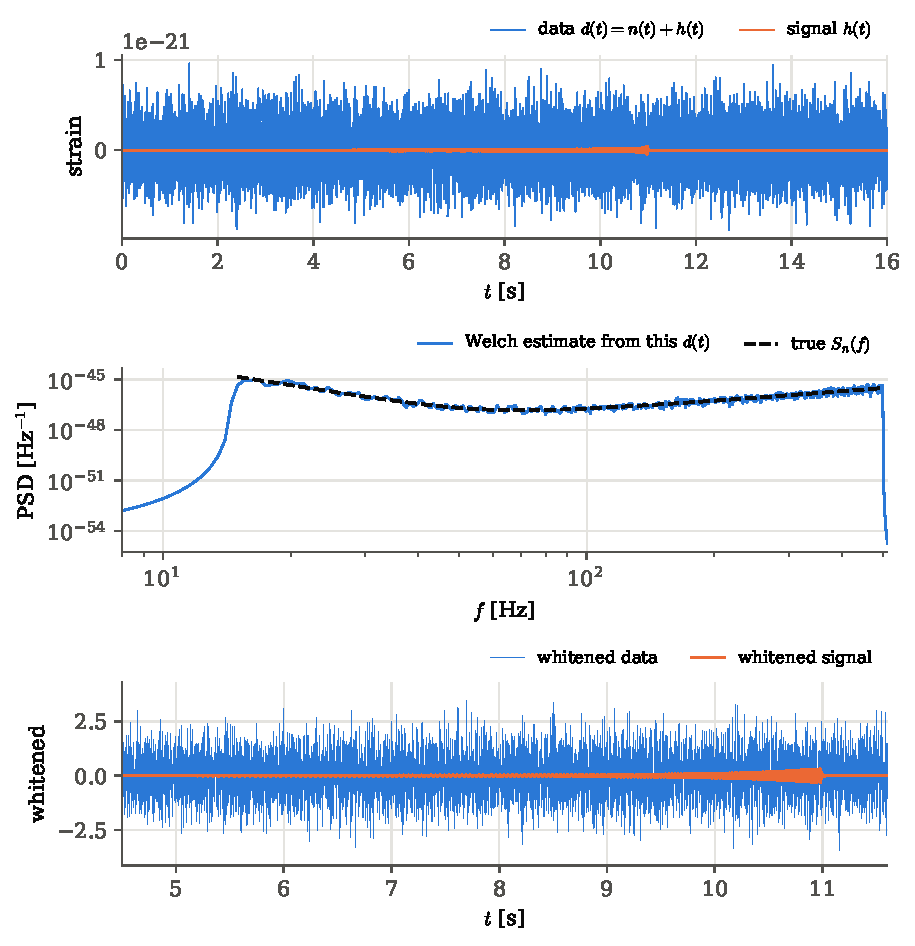
\includegraphics[width=0.85\linewidth]{figures/ch10/det_timeseries.pdf}
\caption{One stretch of simulated detector output with a $\rho=5$ chirp. Top: the data and the signal; the signal
is a small fraction of the noise and cannot be seen. Middle: the spectrum estimated from this stretch alone falls on
the true $S_n(f)$ (dashed). Bottom: after whitening, the noise is flat and the chirp (orange) is still well below it.
Only correlating with the right template brings it out.}
\label{10b:fig:det-timeseries}
\end{figure}

Over $2000$ realisations of each hypothesis (independent noise for the two), the statistic $z$ has mean
$\TenBdetZzeroMean$ and standard deviation $\TenBdetZzeroSd$ under $\Hnull$, and mean $\TenBdetZoneMean$ and
standard deviation $\TenBdetZoneSd$ under $\Halt$, as \eqref{10b:eq:z-dist} predicts
(\cref{10b:fig:det-stats}, left). At a false-alarm probability of $1\%$ the threshold is $z_\alpha=\TenBdetThrZ$,
and the detection probability is $\Phi(5-2.326)=\TenBdetPdZth$; the simulation gives $\TenBdetPdZ$.

\subsection{When the arrival time and phase are unknown}
\label{10b:sec:phase-time}

The test of \cref{10b:sec:matched-filter} was built for a template we know exactly. Imagine running it on a real
detector. A binary that merged somewhere in the Universe sends us a chirp whose shape we can predict from its masses,
but two of its numbers are pure accident: the moment $t_0$ at which it reaches the detector, and the phase $\phi_c$ of
the wave at that moment, which depends on where the two bodies happened to be on their orbit. Neither tells us
anything about the source, and neither can be known in advance. A template with the wrong arrival time lines up its
oscillations against noise; a template with the wrong phase lines up its crests against the signal's troughs. In both
cases the matched filter $(d|h)$ of \eqref{10b:eq:lr} comes out near zero, even with a loud signal in the data.

The question, in words: \emph{must we run a separate matched filter for every phase and every arrival time we can
think of, and if we search over all of them, what does noise alone now produce?} The answer to the first part is no.
The phase costs exactly two filters instead of one, and every arrival time comes out of one Fourier transform. The
answer to the second part is the price we pay for not knowing.

\subsubsection*{The phase}

\emph{The simplest wave first.} Take a pure tone of known amplitude $A$ and angular frequency $\omega$, with an
unknown phase $\phi_c$,
\begin{equation}
  h(t;\phi_c)=A\cos(\omega t+\phi_c).
  \label{10b:eq:tone}
\end{equation}
As a function of $\phi_c$ this looks hopeless: every value of $\phi_c$ is a different waveform. But the addition rule
$\cos(\alpha+\beta)=\cos\alpha\cos\beta-\sin\alpha\sin\beta$, with $\alpha=\omega t$ and $\beta=\phi_c$, separates the
part that depends on time from the part that depends on the phase:
\begin{align}
  h(t;\phi_c)
  &\eqby{1}A\cos\omega t\,\cos\phi_c-A\sin\omega t\,\sin\phi_c
   \eqby{2}h_c(t)\cos\phi_c+h_s(t)\sin\phi_c,
  \label{10b:eq:quadratures}
\end{align}
with $h_c(t)\equiv A\cos\omega t$ and $h_s(t)\equiv-A\sin\omega t$.
\begin{explain}
  \item The addition rule.
  \item Give the two fixed time functions names. All of the dependence on $\phi_c$ is now in the two numbers
        $\cos\phi_c$ and $\sin\phi_c$.
\end{explain}
So every phase is a mixture of the same two waveforms, $h_c$ and $h_s$. They differ by a quarter of a cycle
($-\sin\omega t=\cos(\omega t+\pi/2)$), and are called the two \newterm{quadratures} of the signal.

\emph{The filter of a mixture is the mixture of the filters.} The inner product $(a|b)$ of the working definition
in \cref{10b:sec:noise-fd} is an integral, so it is linear in each slot: $(d\,|\,\alpha a+\beta b)=\alpha(d|a)+\beta(d|b)$
for real numbers $\alpha,\beta$. Applied to \eqref{10b:eq:quadratures},
\begin{equation}
  (d\,|\,h)=x_c\cos\phi_c+x_s\sin\phi_c,
  \qquad x_c\equiv(d\,|\,h_c),\quad x_s\equiv(d\,|\,h_s).
  \label{10b:eq:two-filters}
\end{equation}
The data are correlated with each quadrature once, giving two numbers $x_c$ and $x_s$; the filter for any phase is
then a recombination of these two numbers, with no further reference to the data.

\emph{Which phase fits best?} Treat $(x_c,x_s)$ as a point in a plane and describe it in polar coordinates: its
distance from the origin $r=\sqrt{x_c^2+x_s^2}$ and its angle $\phi_0$, so that $x_c=r\cos\phi_0$ and
$x_s=r\sin\phi_0$. Then
\begin{align}
  (d\,|\,h)
  &\eqby{1}r\cos\phi_0\cos\phi_c+r\sin\phi_0\sin\phi_c
   \eqby{2}r\cos(\phi_c-\phi_0).
  \label{10b:eq:phase-cos}
\end{align}
\begin{explain}
  \item Substitute the polar form of $x_c$ and $x_s$ into \eqref{10b:eq:two-filters}.
  \item The addition rule again, read backwards: $\cos(\phi_c-\phi_0)=\cos\phi_c\cos\phi_0+\sin\phi_c\sin\phi_0$.
\end{explain}
A cosine is at most $1$, and reaches it when its argument is zero. So the best phase is $\phi_c=\phi_0$, the angle of
the point $(x_c,x_s)$, and the filter there equals the distance $r$:
\begin{equation}
  \max_{\phi_c}\,(d\,|\,h)=\sqrt{(d\,|\,h_c)^2+(d\,|\,h_s)^2}.
  \label{10b:eq:phase-max}
\end{equation}
A continuum of phases has been searched with two filters and one square root. The best-fitting phase also comes for
free, as $\phi_0$.

\emph{The two filters as one complex number.} A point in the plane is a complex number, so define
\begin{equation}
  x\equiv x_c+i\,x_s,\qquad |x|=\sqrt{x_c^2+x_s^2}=\max_{\phi_c}(d\,|\,h),\qquad \arg x=\phi_0 .
\end{equation}
In the frequency domain $x$ takes a compact form. We need the Fourier transforms of the two quadratures, in the
convention of \cref{10b:sec:noise-fd}, $\tilde h(f)=\int h(t)\,e^{-2\pi ift}\,\dd t$. Write the two time functions as
complex exponentials,
\begin{equation}
  \cos\omega t=\tfrac12\bigl(e^{i\omega t}+e^{-i\omega t}\bigr),\qquad
  -\sin\omega t=-\tfrac1{2i}\bigl(e^{i\omega t}-e^{-i\omega t}\bigr)=\tfrac i2\bigl(e^{i\omega t}-e^{-i\omega t}\bigr).
\end{equation}
The inner product only uses positive frequencies, and there only the $e^{+i\omega t}$ term contributes. Its
coefficient is $\tfrac12$ for the cosine and $\tfrac i2$ for the sine quadrature. So, at every positive frequency,
\begin{equation}
  \tilde h_s(f)=i\,\tilde h_c(f).
  \label{10b:eq:quad-fd}
\end{equation}
A quarter-cycle delay is multiplication by $i$. Now compute $x_s$ from the definition of the inner product:
\begin{align}
  x_s=(d\,|\,h_s)
  &\eqby{1}4\,\mathrm{Re}\int_0^\infty\frac{\tilde d\,(i\tilde h_c)^*}{S_n}\,\dd f
   \eqby{2}4\,\mathrm{Re}\Bigl[-i\int_0^\infty\frac{\tilde d\,\tilde h_c^*}{S_n}\,\dd f\Bigr]
   \eqby{3}4\,\mathrm{Im}\int_0^\infty\frac{\tilde d\,\tilde h_c^*}{S_n}\,\dd f .
\end{align}
\begin{explain}
  \item The inner product of \cref{10b:sec:noise-fd}, with \eqref{10b:eq:quad-fd}.
  \item $(i\tilde h_c)^*=-i\,\tilde h_c^*$, and the constant $-i$ comes out of the integral.
  \item For any complex number $w=a+ib$, $-iw=b-ia$, so $\mathrm{Re}(-iw)=b=\mathrm{Im}\,w$.
\end{explain}
And $x_c=4\,\mathrm{Re}\int\tilde d\,\tilde h_c^*/S_n\,\dd f$ by definition. Putting the two together,
\begin{equation}
  x=x_c+i\,x_s=4\int_0^\infty\frac{\tilde d(f)\,\tilde h_c^*(f)}{S_n(f)}\,\dd f .
  \label{10b:eq:complex-filter}
\end{equation}
This is the inner product with the ``Re'' left out. Its real part is the cosine filter, its imaginary part the sine
filter, and its modulus is the filter already maximised over the phase.

\emph{From the tone to the chirp.} Nothing above used the fact that the wave was a pure tone, except to find
\eqref{10b:eq:quad-fd}. For the stationary-phase chirp of \cref{T2a:eq:hf}, $\tilde h(f)=\mathcal Af^{-7/6}e^{-i\Psi(f)}$ with $\Psi(f)=2\pi ft_c-\phi_c-\pi/4+\dots$ (\cref{T2g:sec:tc-phic}),
the unknown phase enters $\Psi$ as an additive constant, so it multiplies the whole Fourier transform by one factor
$e^{i\phi_c}=\cos\phi_c+i\sin\phi_c$. That is \eqref{10b:eq:quadratures} again, with $\tilde h_c$ the template at
$\phi_c=0$ and $\tilde h_s=i\tilde h_c$. The complex filter \eqref{10b:eq:complex-filter} therefore searches all phases
of the chirp as well. (With $-\phi_c$ inside $\Psi$ and $e^{-i\Psi}$ outside, the factor is $e^{+i\phi_c}$; the opposite convention would only flip the sign of $\phi_0$.)

\subsubsection*{The arrival time}

\emph{A delay is a phase that grows with frequency.} A signal arriving $t_0$ later is the same waveform shifted,
$h(t)\to h(t-t_0)$. Its Fourier transform is
\begin{align}
  \int h(t-t_0)\,e^{-2\pi ift}\,\dd t
  &\eqby{1}\int h(s)\,e^{-2\pi if(s+t_0)}\,\dd s
   \eqby{2}e^{-2\pi ift_0}\,\tilde h(f).
  \label{10b:eq:shift}
\end{align}
\begin{explain}
  \item Substitute $s=t-t_0$, so $t=s+t_0$ and $\dd t=\dd s$.
  \item The factor $e^{-2\pi ift_0}$ does not depend on $s$ and comes out; what is left is $\tilde h(f)$.
\end{explain}
Put the shifted template into the complex filter \eqref{10b:eq:complex-filter}. The complex conjugate turns
$e^{-2\pi ift_0}$ into $e^{+2\pi ift_0}$:
\begin{equation}
  x(t_0)=4\int_0^\infty\frac{\tilde d(f)\,\tilde h_c^*(f)}{S_n(f)}\,e^{+2\pi ift_0}\,\dd f
        =\int_0^\infty Q(f)\,e^{+2\pi ift_0}\,\dd f,
  \qquad Q(f)\equiv\frac{4\,\tilde d(f)\,\tilde h_c^*(f)}{S_n(f)} .
  \label{10b:eq:filter-t0}
\end{equation}

\emph{One transform for all arrival times.} Look at what depends on what. $Q(f)$ is built from the data, the template
and the noise spectrum; it does not know about $t_0$, so it is computed once. The arrival time appears only in
$e^{+2\pi ift_0}$, and an integral of a function of $f$ against $e^{+2\pi ift_0}$ is, by definition, the inverse
Fourier transform of that function, evaluated at the time $t_0$. So
\begin{equation}
  x(t_0)=\mathcal F^{-1}[Q](t_0)\quad\text{for every }t_0\text{ at once.}
\end{equation}
On a stretch of $N$ samples there are $N$ possible arrival times. Filtering at each one separately would take $N$
operations per lag, $N^2$ in all; the fast Fourier transform delivers all $N$ values in about $N\log_2N$. For the
$\TenBdetNlags$ lags of our example that is about a thousand times less work per template,
and it is how real searches work \cite{AllenFINDCHIRP2012}. In the script, \texttt{q} is $Q(f)$ on the frequency grid
(zero outside the band), \texttt{x} is $x(t_0)$ on every lag, and the statistic maximised over both unknowns,
$z_{\max}=\max_{t_0}|x(t_0)|/\rho$, is stored:

\pyfile[firstline=103,lastline=107,firstnumber=103]{code/ch10/08_detection.py}{The filter at every arrival time}

\subsubsection*{What noise alone now gives}

Searching costs something. Every time we try another phase or another arrival time, we give the noise another chance
to look like a signal. To set a threshold we need the distribution of $z_{\max}$ when the data are noise alone, $d=n$.

\emph{One arrival time.} Fix $t_0$. Under $\Hnull$ the two filters are $x_c=(n|h_c)$ and $x_s=(n|h_s)$. By
\eqref{10b:eq:noise-overlap}, each is Gaussian with mean zero, and their variances and covariance are inner products of
the templates. These follow from \eqref{10b:eq:quad-fd}:
\begin{align}
  (h_s\,|\,h_s)&\eqby{1}4\int_0^\infty\frac{|i\tilde h_c|^2}{S_n}\,\dd f\eqby{2}(h_c\,|\,h_c)=\rho^2,\nonumber\\
  (h_c\,|\,h_s)&\eqby{3}4\,\mathrm{Re}\Bigl[-i\int_0^\infty\frac{|\tilde h_c|^2}{S_n}\,\dd f\Bigr]\eqby{4}0 .
\end{align}
\begin{explain}
  \item The inner product of a signal with itself; the real part is not needed because $|\cdot|^2$ is real.
  \item $|i|=1$; and $(h_c|h_c)=\rho^2$ is the optimal signal-to-noise ratio of the working definition.
  \item The same manipulation as for $x_s$ above, with $\tilde d$ replaced by $\tilde h_c$.
  \item The integral is a real number, so $-i$ times it is purely imaginary, and its real part vanishes.
\end{explain}
So $x_c/\rho$ and $x_s/\rho$ are Gaussians with mean zero, variance one and covariance zero. For jointly Gaussian
variables zero covariance means independence, so they are two independent $\Normal(0,1)$ variables, and
\begin{equation}
  \frac{|x|^2}{\rho^2}=\Bigl(\frac{x_c}{\rho}\Bigr)^2+\Bigl(\frac{x_s}{\rho}\Bigr)^2\sim\chi^2_2
\end{equation}
is the sum of the squares of two independent unit Gaussians, a $\chi^2$ with two degrees of freedom
(\cref{2b:sec:chi2-many}). With $p=2$ the $\chi^2_p$ density \eqref{2b:eq:chi2} becomes simply $\tfrac12e^{-v/2}$, an
exponential, so its tail is $\Prob(\chi^2_2>v)=\int_v^\infty\tfrac12e^{-v'/2}\dd v'=e^{-v/2}$. With $v=u^2$,
\begin{equation}
  \Prob\Bigl(\frac{|x|}{\rho}>u\,\Big|\,\Hnull\Bigr)=e^{-u^2/2}.
  \label{10b:eq:rayleigh-tail}
\end{equation}
Compare the known-phase test: there $\Prob(z>u)$ was a one-sided Gaussian tail, about $e^{-u^2/2}/(u\sqrt{2\pi})$ for
large $u$. Searching over the phase has raised the false-alarm probability by a factor of about $u\sqrt{2\pi}$, roughly
$6$ at $u=2.5$: the price of one unknown angle.

\emph{All arrival times.} Now we take the largest $|x(t_0)|/\rho$ over all $N=\TenBdetNlags$ lags. If the lags were
independent, the largest would stay below $u$ only if every one did:
\begin{equation}
  \Prob(z_{\max}>u\given\Hnull)=1-\bigl(1-e^{-u^2/2}\bigr)^{N}\approx N\,e^{-u^2/2}
  \quad\text{while this is small}.
  \label{10b:eq:max-lags}
\end{equation}
This is the look-elsewhere effect of \cref{ch:04}: the largest of many noise
peaks is larger than a typical one, and a threshold that was safe for one trial is not safe for $N$. The simulation
shows how large the effect is. Under $\Hnull$ the median of $z_{\max}$ is $\TenBdetMzeroMed$, the $1\%$ threshold
rises from $z_\alpha=\TenBdetThrZ$ to $\TenBdetThrM$, and for the same $\rho=5$ the detection probability falls from
$\TenBdetPdZ$ to $\TenBdetPdM$ (\cref{10b:fig:det-stats}, middle and right).

\emph{How many trials, really?} The lags are not independent: the filter output is smooth over a time about the
inverse of the bandwidth, so neighbouring lags see nearly the same noise. We can measure how many independent trials
the search is worth by solving \eqref{10b:eq:max-lags} for $N$ at the measured threshold, $N_{\rm eff}e^{-u^2/2}=0.01$.
This gives $N_{\rm eff}\approx\TenBdetNeff$, fewer than the $\TenBdetNlags$ lags. It is a rough number: the
$1\%$ threshold rests on the twenty largest of the $2000$ noise-only values, and $N_{\rm eff}$ grows as $e^{u^2/2}$,
so a small error in $u$ becomes a large one in $N_{\rm eff}$.

The lesson, in one line: not knowing when and in what phase a signal arrives costs nothing in computation (two
filters and one Fourier transform) but a great deal in significance, because noise alone now gets thousands of
chances. This is why ground-based searches demand $\rho\gtrsim8$ before claiming a detection, and why LISA forecasts
assume a threshold near $\rho\approx15$ for these long signals \cite{Coogan2022}.

\begin{figure}[htbp]
\centering
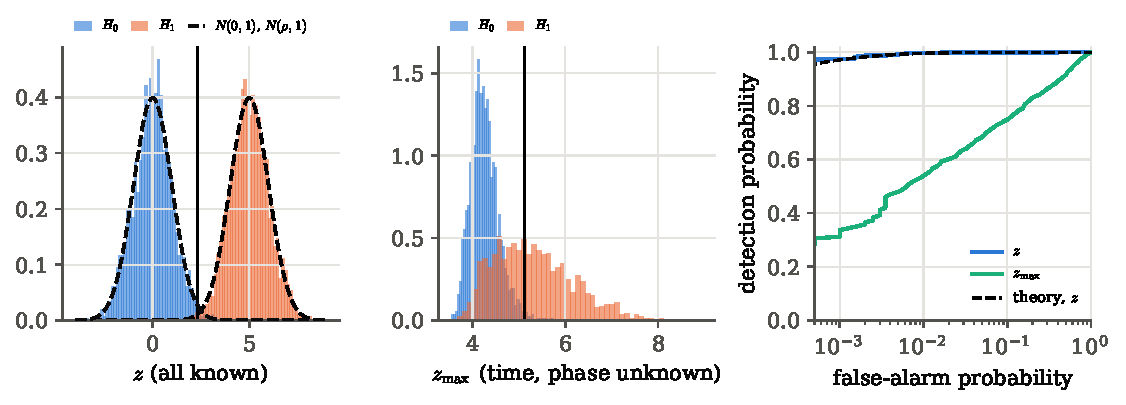
\includegraphics[width=\linewidth]{figures/ch10/det_stats.pdf}
\caption{Sampling distributions of the detection statistic over $2000$ noise realisations, $\rho=5$. Left: with
the template, time and phase known, $z$ is $\Normal(0,1)$ under $\Hnull$ and $\Normal(\rho,1)$ under $\Halt$
(dashed); the vertical line is the $1\%$ false-alarm threshold. Middle: maximising over arrival time and phase
pushes the noise-only distribution up, and the threshold with it. Right: detection probability against
false-alarm probability (receiver operating characteristic); the price of not knowing $t_0$ and $\phi_c$ is the
gap between the two curves.}
\label{10b:fig:det-stats}
\end{figure}

\subsection{Whitening, and what one stretch can tell us about the spectrum}
\label{10b:sec:welch}

Everything above rests on the claim that each Fourier mode of the noise is a complex Gaussian of variance
$\sigma_k^2=\tfrac T2S_n(f_k)$ (\cref{10b:eq:mode-variance}). Two practical questions follow at once. How do we
look at the data so that this claim can be checked? And if the spectrum is not known, what does one stretch of data say about it?

\emph{Whitening.} Divide each mode by its own standard deviation, $w_k=\tilde n_k/\sigma_k$. Then
$\E|w_k|^2=1$ in every bin, however steep the spectrum: the noise has become equally loud at all frequencies,
\newterm{white}. The same division turns the noise-weighted inner product into an ordinary dot product. For two
signals with whitened modes $a_k=\tilde a_k/\sigma_k$, $b_k=\tilde b_k/\sigma_k$,
\begin{equation}
  (a\,|\,b)=4\Delta f\sum_k\frac{\mathrm{Re}\,\tilde a_k\tilde b_k^*}{S_n(f_k)}
  \eqby{1}2\sum_k\mathrm{Re}\,\big(a_kb_k^*\big),
  \label{10b:eq:whitened-ip}
\end{equation}
\begin{explain}
  \item $\sigma_k^2=T S_n(f_k)/2$ and $\Delta f=1/T$, so $\mathrm{Re}(\tilde a_k\tilde b_k^*)/\sigma_k^2=2\Delta f\,\mathrm{Re}(\tilde a_k\tilde b_k^*)/S_n(f_k)$.
\end{explain}
so in whitened data the filter $(d|h)$ is a plain correlation between the whitened data and the whitened template,
and $(n|n)=2\sum_k|w_k|^2$ is the sum of squares of independent unit-variance numbers, as in
\eqref{10b:eq:noise-density}. This is what the bottom panel of \cref{10b:fig:det-timeseries} shows.

\emph{What one stretch says about the spectrum.} The natural estimate of $\sigma_k^2$ from one stretch is the
\newterm{periodogram} of that bin, $|\tilde n_k|^2$. Its distribution follows from \eqref{10b:eq:mode-variance}: the real
and imaginary parts of $\tilde n_k$ are independent Gaussians of variance $\sigma_k^2/2$, so with $a$ and $b$ two
independent $\Normal(0,1)$ variables,
\begin{equation}
  \frac{|\tilde n_k|^2}{\sigma_k^2}=\frac{a^2+b^2}{2}=\tfrac12\chi^2_2,
  \qquad\text{density }e^{-v},\ \ v\ge0,
  \label{10b:eq:periodogram}
\end{equation}
the exponential distribution (the $\chi^2_2$ density is $\tfrac12e^{-v/2}$, as used for \eqref{10b:eq:rayleigh-tail}).
An exponential has its standard deviation equal to its mean. So a single-bin periodogram is right on average but is
wrong by $100\%$ in any one realisation, and a longer stretch does not help: it only supplies more bins, each as noisy as
before. The way to a good estimate is to average. Cut the data into $M$ segments, compute the periodogram of each
and average the $M$ values in each bin (Welch's method). The sum of $M$ independent exponentials is a gamma
variable of mean $M$ and variance $M$, so the average has mean one and variance $1/M$: the fractional error falls as
$1/\sqrt M$. This sum is exactly the quantity $Q$ of the next subsection.

Cutting the data into segments has a price. Each segment is the product of the signal with a rectangular window, and in
the Fourier domain a product is a convolution: the loud low-frequency part of the spectrum leaks, through the slowly
decaying wings of the window's transform, into frequency bins where the true noise is orders of magnitude lower. For
detector noise that spans many decades the leakage can dominate the estimate. Segments are therefore multiplied by a
smooth taper that falls to zero at the ends (for example a Tukey or Hann window), which suppresses the wings, and
overlapping segments recover the information the taper discards. In the script,
the periodograms of $400$ simulated noise realisations in the band have mean $\TenBwhMean$ and variance
$\TenBwhVar$ in units of $\sigma_k^2$, as \eqref{10b:eq:periodogram} requires; a Kolmogorov--Smirnov test against the
exponential gives $p=\TenBwhKSp$; and the real parts of the whitened modes have standard deviation $\TenBwhReSd$ and
excess kurtosis $\TenBwhReKurt$, as for a Gaussian of variance one half per component after the factor $\sqrt2$
(\pyname{16_whiten_chi2.py}). On real data the same two checks, an exponential periodogram and Gaussian
whitened modes, are what tells us the Gaussian stationary noise model is adequate, or that glitches and drifts are
present.

\subsection{When the noise spectrum is itself estimated}
\label{10b:sec:psd}

The likelihood \eqref{10b:eq:gw-like} assumed $S_n$ known. It never is: it is estimated from data near the event,
for instance by averaging $|\tilde n_k|^2$ over $M$ stretches without a signal. Plugging the estimate $\hat S_n$
into the Gaussian likelihood treats a noisy number as exact. What should we do instead?

\emph{The question in words.} What is the probability of the on-source residual in one frequency bin, regardless of
the true noise level in that bin, given what the off-source stretches told us about that level? It is a marginal:
the true variance is a nuisance, and we integrate it out, exactly as $V$ was integrated out to obtain Student's $t$
in \cref{ch:02}.

\emph{Ingredients.} In bin $k$ write $s=\E|\tilde n_k|^2$ for the unknown true variance, $r=\tilde d_k-\tilde h_k$
for the on-source residual, and $x_1,\dots,x_M$ for the same bin in $M$ off-source stretches. Each is a complex
Gaussian of variance $s$. With the prior $p(s)\propto1/s$ (scale-free, \cref{ch:05}), the off-source data give the
posterior
\begin{align}
  p(s\given x)
  &\eqby{1}\frac{\prod_m\frac1{\pi s}e^{-|x_m|^2/s}\cdot\frac1s}{\int(\cdots)\dd s}
   \eqby{2}\frac{Q^M}{\Gamma(M)}\,s^{-M-1}e^{-Q/s},\qquad Q\equiv\sum_{m=1}^M|x_m|^2\equiv M\hat s .
  \label{10b:eq:invgamma}
\end{align}
\begin{explain}
  \item Bayes' theorem with the complex-Gaussian density of each stretch and the prior $1/s$.
  \item Collect $s^{-M}\cdot s^{-1}$ and $e^{-\sum|x_m|^2/s}$; the normalisation is the gamma integral
        $\int_0^\infty s^{-a-1}e^{-Q/s}\dd s=\Gamma(a)/Q^a$ (substitute $y=Q/s$), with $a=M$. $\hat s$ is the
        averaged estimate of the variance.
\end{explain}
\emph{Marginalise.} The density of the on-source residual, regardless of $s$, is
\begin{align}
  p(r\given x)
  &\eqby{1}\int_0^\infty\frac{1}{\pi s}e^{-|r|^2/s}\,p(s\given x)\,\dd s
   \eqby{2}\frac{Q^M}{\pi\Gamma(M)}\int_0^\infty s^{-M-2}e^{-(Q+|r|^2)/s}\dd s\nonumber\\
  &\eqby{3}\frac{Q^M}{\pi\Gamma(M)}\,\frac{\Gamma(M+1)}{(Q+|r|^2)^{M+1}}
   \eqby{4}\frac{1}{\pi\hat s}\Big(1+\frac{|r|^2}{M\hat s}\Big)^{-(M+1)} .
  \label{10b:eq:student-gw}
\end{align}
\begin{explain}
  \item Marginalisation over the nuisance $s$.
  \item Insert \eqref{10b:eq:invgamma} and collect the powers of $s$: $s^{-1}s^{-M-1}=s^{-M-2}$.
  \item The same gamma integral with $a=M+1$ and $Q\to Q+|r|^2$.
  \item $\Gamma(M+1)/\Gamma(M)=M$; divide numerator and denominator by $Q^{M+1}$ and use $Q=M\hat s$.
\end{explain}
This is a two-dimensional Student-$t$ (with $\nu=2M$ and $t^2=2|r|^2/\hat s$ it reads
$(1+t^2/\nu)^{-(\nu+2)/2}$) \cite{RoverMeyerChristensen2011}. As $M\to\infty$,
$(1+x/M)^{-(M+1)}\to e^{-x}$ with $x=|r|^2/\hat s$: the Gaussian likelihood with the estimate is recovered, because
the estimate has become exact. For finite $M$ the tails are heavier. A residual that is large compared with
$\hat s$ is no longer catastrophic, because it may mean that the noise in that bin was underestimated.

\paragraph{Example: what the plug-in costs.} The script estimates the amplitude of the known chirp ($\rho=5$, true
amplitude one) in $2000$ experiments, each with its own $M$ off-source stretches, in two ways: the Gaussian
likelihood with $\hat S_n$ plugged in (maximum-likelihood estimate and its curvature error) and the Student-$t$
likelihood \eqref{10b:eq:student-gw} summed over bins (posterior on a grid). The amplitude is in units of the true
one, so the ideal error is $1/\rho$; we quote widths and scatters times $\rho$.

\begin{center}
\small
\begin{tabular}{@{}rcccccc@{}}
\toprule
& \multicolumn{3}{c}{Gaussian, $\hat S_n$ plugged in} & \multicolumn{3}{c}{Student-$t$, $S_n$ marginalised}\\
\cmidrule(lr){2-4}\cmidrule(l){5-7}
$M$ & claimed width & actual scatter & coverage & claimed width & actual scatter & coverage\\\midrule
2  & $\TenBwidGTwo$ & $\TenBsdGTwo$ & $\TenBcovGTwo\%$ & $\TenBwidTTwo$ & $\TenBsdTTwo$ & $\TenBcovTTwo\%$\\
4  & $\TenBwidGFour$ & $\TenBsdGFour$ & $\TenBcovGFour\%$ & $\TenBwidTFour$ & $\TenBsdTFour$ & $\TenBcovTFour\%$\\
8  & $\TenBwidGEight$ & $\TenBsdGEight$ & $\TenBcovGEight\%$ & $\TenBwidTEight$ & $\TenBsdTEight$ & $\TenBcovTEight\%$\\
16 & $\TenBwidGSixteen$ & $\TenBsdGSixteen$ & $\TenBcovGSixteen\%$ & $\TenBwidTSixteen$ & $\TenBsdTSixteen$ & $\TenBcovTSixteen\%$\\
32 & $\TenBwidGThirtyTwo$ & $\TenBsdGThirtyTwo$ & $\TenBcovGThirtyTwo\%$ & $\TenBwidTThirtyTwo$ & $\TenBsdTThirtyTwo$ & $\TenBcovTThirtyTwo\%$\\
\bottomrule
\end{tabular}
\end{center}

\noindent Read the plug-in columns first. The claimed width is too small, by a factor close to
$\sqrt{(M-1)/M}$ ($0.707$ for $M=2$). The reason is Jensen's inequality: $\hat s$ is unbiased, but
$\E[1/\hat s]=\frac{M}{M-1}\frac1s$ is not, so $(h|h)$ computed with $\hat S_n$ is too large on average. Worse, the
actual scatter of the estimate is larger than the ideal one, because a bin whose noise was underestimated by chance
receives too much weight. Both effects push the coverage of the nominal $68.3\%$ interval down to $\TenBcovGTwo\%$
for $M=2$. The Student-$t$ likelihood gives a more robust estimate (its scatter is half as large at $M=2$) and an
interval closer to honest. What it cannot do is recover information that was never measured: with only two
off-source stretches per bin, thousands of separately uncertain noise levels still cost coverage (the Monte Carlo
error of each coverage is $\pm\TenBcovMCerr\%$). Both methods converge for $M\gtrsim16$
(\cref{10b:fig:det-psdcov}). Research analyses therefore estimate the spectrum from long stretches, or describe it
by a smooth model with few parameters fitted together with the signal
\cite{CornishLittenberg2015,LittenbergCornish2023}.

\begin{figure}[htbp]
\centering
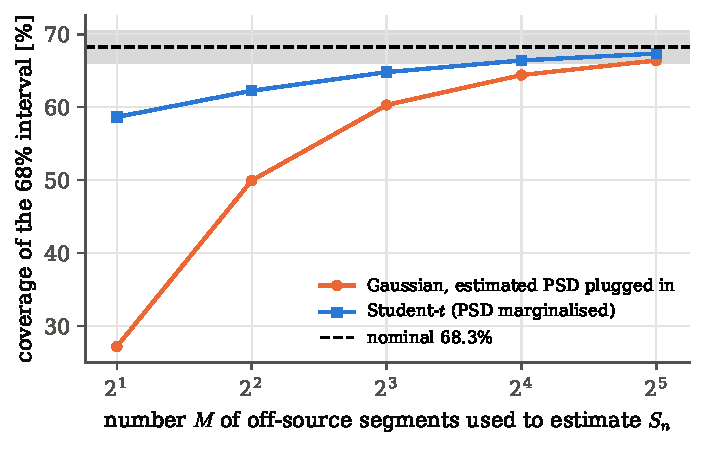
\includegraphics[width=0.66\linewidth]{figures/ch10/det_psdcov.pdf}
\caption{Coverage of the nominal $68.3\%$ interval on the signal amplitude when $S_n$ is estimated from $M$
off-source stretches, over $2000$ experiments (grey band: $\pm2$ Monte Carlo standard errors). Plugging the
estimate into the Gaussian likelihood is overconfident for small $M$; marginalising the unknown spectrum (Student-$t$)
recovers most of the gap.}
\label{10b:fig:det-psdcov}
\end{figure}

\begin{pitfall}[A plugged-in spectrum is an overconfident spectrum]
An unbiased estimate of $S_n$ gives a biased estimate of $1/S_n$, the quantity the likelihood actually uses. With
few averages the plug-in Gaussian likelihood claims error bars too small by $\sqrt{(M-1)/M}$ and lets badly
estimated bins dominate. Either average many stretches, or marginalise the spectrum.
\end{pitfall}

\subsection{A signal must have the right shape: the $\chi^2$ consistency test}
\label{10b:sec:chi2}

A large filter output does not prove a gravitational wave. A short burst of instrumental noise (a glitch) can also
correlate with the template and give a large $z$. What a glitch lacks is the \emph{shape} of the chirp: the template
predicts how the signal-to-noise ratio should be shared among frequency bands, and a burst puts its power
somewhere else. That prediction is a test with a known distribution.

\emph{The question in words.} Having found a peak of the filter $x(t_0)$ at some lag, is the way $x$ was built up
across frequency what the template predicts, up to noise? Split the band into $p$ pieces with edges chosen so that
each carries the same share of the signal-to-noise ratio, $\rho_i^2=\rho^2/p$ (possible because $4|\tilde h|^2/S_n$
is positive). Let $x_i$ be the complex filter \eqref{10b:eq:complex-filter} restricted to piece $i$, so
$\sum_ix_i=x$. For the true signal and noise,
\begin{equation}
  \E\,x_i=\frac{\rho^2}{p}\,e^{i\phi_0}=\frac{\E\,x}{p},
\end{equation}
because the signal's filter output accumulates $\rho_i^2$ in piece $i$. So the residuals $r_i=x_i/\rho-x/(p\rho)$ have
zero mean when the data contain the template (or only noise). Their noise is Gaussian: by \eqref{10b:eq:noise-overlap}
the real and imaginary parts of $x_i/\rho$ each have variance $\rho_i^2/\rho^2=1/p$. The $2p$ real numbers
$\mathrm{Re}\,r_i,\mathrm{Im}\,r_i$ therefore have variance $1/p$ each, and two linear constraints, $\sum_i\mathrm{Re}\,r_i=0$ and
$\sum_i\mathrm{Im}\,r_i=0$ (the sum of the residuals is zero by construction), so
\begin{equation}
  \chi^2\equiv p\sum_{i=1}^p|r_i|^2\sim\chi^2_{2p-2}.
  \label{10b:eq:chi2veto}
\end{equation}
A sum of squares of $2p$ unit Gaussians would be $\chi^2_{2p}$; each linear constraint removes one degree of freedom
(the same count as the $n-1$ of the sample variance in \cref{ch:02}). A glitch correlates with the template mainly
in the band where it has power, so one $x_i$ is far from $x/p$ and $\chi^2$ is large.

\emph{What the simulation shows.} The script (\pyname{16_whiten_chi2.py}) divides the chirp band into $p=\TenBchiP$ pieces
($2p-2=\TenBchiDof$ degrees of freedom), finds the lag of the largest $|x|$ and evaluates \eqref{10b:eq:chi2veto} there.
For noise alone the mean is $\TenBchiNoiseMean$, a little below $\TenBchiDof$ because the lag was chosen to be the
one where the pieces happen to line up; for a true chirp of $\rho=10$ it is $\TenBchiSigMean$ and the fraction below the
$0.1\%$ threshold $\TenBchiThr$ is $\TenBchiSigPass\%$. Now take a short burst at $60$\,Hz, placed at the moment the chirp passes that frequency, and scaled to the same
optimal signal-to-noise ratio as the chirp, $\rho=10$. The template matches it only in part: the median $|x|/\rho$ is
$\TenBchiBurstZ$, well above the $\TenBchiNoiseZ$ of noise alone but below the $\TenBchiSigZ$ of the chirp. Many such
bursts would pass a threshold on the filter output alone. Its median $\chi^2$ is $\TenBchiBurstMed$, and only $\TenBchiBurstPass\%$ of the bursts
fall below the threshold (\cref{10b:fig:det-chi2}, left). The test does not make the matched filter better; it rejects
the large values of $z$ that come from something other than the template, and detection pipelines weight their statistic by it.

\begin{figure}[htbp]
\centering
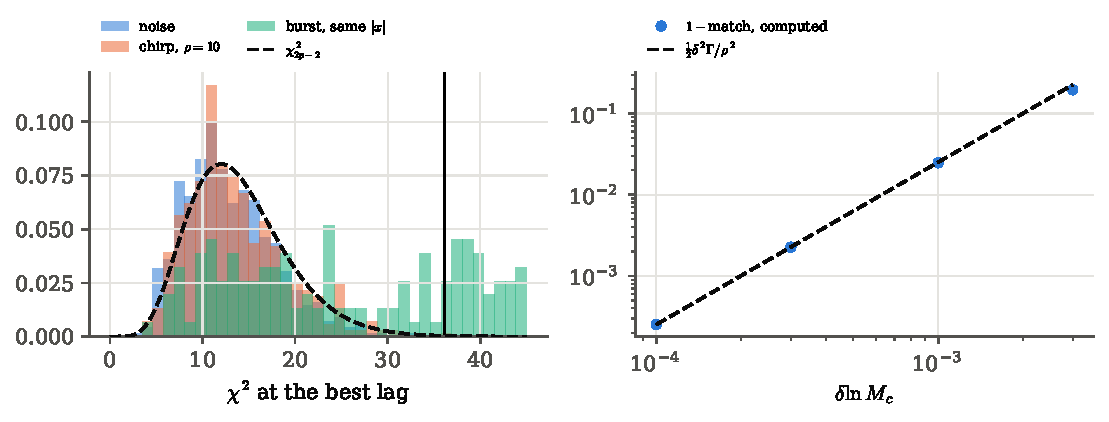
\includegraphics[width=\linewidth]{figures/ch10/det_chi2.pdf}
\caption{Left: the $\chi^2$ statistic of \eqref{10b:eq:chi2veto} at the best lag, for noise alone, for a chirp of
$\rho=10$ (both follow $\chi^2_{14}$, dashed) and for a narrow-band burst with a similar filter output, which does not.
The vertical line is the $0.1\%$ threshold. Right: one minus the match between two chirps whose chirp masses (the mass combination of \cref{T2a:eq:Pf} that sets the sweep) differ by
$\delta\ln M_c$, against the Fisher expansion of \cref{10b:sec:metric}.}
\label{10b:fig:det-chi2}
\end{figure}

\paragraph{What this buys the rest of the chapter.} Once a signal is detected, the same likelihood
\eqref{10b:eq:gw-like}, now read as a function of $\params$, is what parameter estimation explores. Its peak is the
best fit and its width is the error. The expected curvature of its logarithm at the true parameters is the Fisher
matrix of \cref{10a:sec:fisher}, and for this likelihood it takes a particularly transparent form.
\section{The Fisher matrix of a chirp}
\label{10b:sec:fisher}

Suppose LISA has detected the inspiral. The likelihood \eqref{10b:eq:gw-like} of \cref{10b:sec:detection},
$p(\data\given\params)\propto e^{-(d-h(\params)|d-h(\params))/2}$, now becomes a function on parameter space, and
its peak sits close to the true masses, arrival time and phase (the chirp mass, the coalescence time $t_c$ and the
coalescence phase $\phi_c$ of the chirp, \cref{T2a:sec:chirp,T2g:sec:tc-phic}). How sharp will that peak be? That is what a mission
designer, or a theorist asking whether a dark-matter spike could ever be seen, needs before the data exist. In
\cref{10a:sec:fisher} the answer was the Fisher matrix, the expected curvature of $-\ln\Like$ at the true
parameters. For the gravitational-wave likelihood it turns into a short, transparent formula, and that formula
explains in one picture why some parameters are measured to a part in ten million and others to tens of per cent.

\subsection{From the likelihood to \texorpdfstring{$\Gamma_{ij}=(\partial_ih|\partial_jh)$}{Gamma = (d_i h | d_j h)}}
\label{10b:sec:fisher-derive}

\emph{The question in words.} If the data were generated by the true parameters $\params_0$ with a typical noise
realisation, how quickly would $\ln\Like$ fall as we move away from $\params_0$? Differentiate
$\ln\Like=-\tfrac12(d-h|d-h)$ twice, using that the inner product is bilinear and symmetric, and write
$\partial_i\equiv\partial/\partial\theta_i$:
\begin{align}
  -\partial_i\partial_j\ln\Like
  &\eqby{1}-\partial_j\big(d-h\,\big|\,\partial_ih\big)
   \eqby{2}\big(\partial_jh\,\big|\,\partial_ih\big)-\big(d-h\,\big|\,\partial_i\partial_jh\big),\nonumber\\
  \Gamma_{ij}\equiv\E\big[-\partial_i\partial_j\ln\Like\big]_{\params_0}
  &\eqby{3}\big(\partial_ih\,\big|\,\partial_jh\big)-\E\big(n\,\big|\,\partial_i\partial_jh\big)
   \eqby{4}\big(\partial_ih\,\big|\,\partial_jh\big).
  \label{10b:eq:gw-fisher}
\end{align}
\begin{explain}
  \item $\partial_i(d-h|d-h)=-2(d-h|\partial_ih)$, because only $h$ depends on $\params$.
  \item Product rule: the derivative hits either $d-h$ (giving $-\partial_jh$) or $\partial_ih$.
  \item At the true parameters $d-h(\params_0)=n$, the noise.
  \item $(n|a)$ has mean zero for any fixed signal $a$ \eqref{10b:eq:noise-overlap}.
\end{explain}
This is the \newterm{Fisher information matrix} of gravitational-wave astronomy,
$\Gamma_{ij}=(\partial h/\partial\theta_i\,|\,\partial h/\partial\theta_j)$ \cite[eq.~(10)]{CutlerFlanagan1994},
\cite[eq.~(41)]{BarackCutler2004}, written $\Gamma$ by tradition where \cref{10a:sec:fisher} wrote $\Fish$. Its other
face, the covariance of the score, gives the same: the score is $S_i=\partial_i\ln\Like=(n|\partial_ih)$ at the
truth, and by \eqref{10b:eq:noise-overlap} $\E[S_iS_j]=(\partial_ih|\partial_jh)$.

It is also the Gaussian formula \eqref{10a:eq:gauss-fisher} of \cref{10a:sec:gauss} in disguise. Take as data
vector the real and imaginary parts of all Fourier modes. Their means are $\mathrm{Re}\,\tilde h_k$ and
$\mathrm{Im}\,\tilde h_k$, their covariance is diagonal with entries $\sigma_k^2/2=\tfrac T4S_n(f_k)$ \eqref{10b:eq:mode-variance}, with $S_n$ the
detector's noise spectrum (for LISA \cref{T2a:eq:Sn}), and the
covariance does not depend on $\params$. So the trace term vanishes and the mean term is
$\sum_k[\mathrm{Re}\,\partial_i\tilde h_k\,\mathrm{Re}\,\partial_j\tilde h_k+\mathrm{Im}\,\partial_i\tilde h_k\,
\mathrm{Im}\,\partial_j\tilde h_k]/(\sigma_k^2/2)=4\Delta f\sum_k\mathrm{Re}(\partial_i\tilde h_k\,\partial_j\tilde h_k^*)
/S_n(f_k)$, which is $(\partial_ih|\partial_jh)$. All information sits in the mean channel, because the detector noise
does not care what the source is. Then, exactly as before, $\bm\Sigma=\Gamma^{-1}$ is the forecast covariance and
$\sqrt{\Sigma_{ii}}$ the marginalised error of $\theta_i$ \cite[eq.~(11)]{CutlerFlanagan1994}.

\subsection{The signal model and its derivatives}
\label{10b:sec:signal-model}

The waveform is the stationary-phase chirp derived in \cref{T2a:sec:spa}, $\tilde h(f)=\mathcal Af^{-7/6}e^{-i\Psi(f)}$:
the Fourier transform of the inspiral, in which each frequency is built by the short stretch of the chirp that passes
through it, with amplitude $\mathcal A$ \eqref{T2a:eq:hf} and phase $\Psi$. We carry the phase to the order at which the mass ratio first appears. Cutler and Flanagan's restricted
post-Newtonian (PN) phase (an expansion in powers of $(v/c)^2$, with $v$ the orbital speed, \cref{T2g:sec:pn}) \cite[eq.~(42)]{CutlerFlanagan1994} is, in our sign convention (the footnote to
\cref{T2a:eq:spa} explains why theirs has $e^{+i\Psi}$),
\begin{equation}
\begin{aligned}
  \Psi(f)&=2\pi ft_c-\phi_c-\frac\pi4+\frac{3}{128}\,u^{-5/3}\Big[1+\frac{20}{9}\Big(\frac{743}{336}+\frac{11}{4}\eta\Big)x
  -16\pi x^{3/2}\Big],\\
  u&=\frac{\pi G\mathcal Mf}{c^3},\qquad x=u^{2/3}\eta^{-2/5}.
\end{aligned}
  \label{10b:eq:psi-pn}
\end{equation}
The Newtonian term is \cref{T2a:eq:psiN}: $t_c$ and $\phi_c$ are the time and phase at which the binary would
coalesce (\cref{T2g:sec:tc-phic}), and $\mathcal M$ is the chirp mass, the one combination of the two masses that
sets the Newtonian sweep \eqref{T2a:eq:Pf}. The bracket adds the first and the 1.5PN corrections, derived term by term
in \cref{T2g:sec:pn} as \eqref{T2g:eq:psi-pn}, with $u$ the reduced frequency of \eqref{T2g:eq:u}. Here
$x=(\pi GMf/c^3)^{2/3}$ is $(v/c)^2$ with the total mass $M=\mathcal M\eta^{-3/5}$, and
$\eta=m_1m_2/M^2$ is the symmetric mass ratio (\unpack{$\eta=1/4$ for equal masses, $\eta\approx m_2/m_1$ when one is
much lighter}). The parameters are
$\params=(\ln\mathcal M,\ln\eta,t_c,\phi_c,\ln\mathcal A)$; logarithms make the errors fractional.

The derivatives are short because every parameter but one sits in the phase. With $\tilde h=\mathcal Af^{-7/6}e^{-i\Psi}$,
\begin{equation}
  \frac{\partial\tilde h}{\partial\ln\mathcal A}=\tilde h,
  \qquad
  \frac{\partial\tilde h}{\partial\theta}=-i\,\frac{\partial\Psi}{\partial\theta}\,\tilde h
  \quad\text{for }\theta\in\{\ln\mathcal M,\ln\eta,t_c,\phi_c\},
  \label{10b:eq:derivs}
\end{equation}
with $\partial\Psi/\partial t_c=2\pi f$, $\partial\Psi/\partial\phi_c=-1$, and the mass derivatives obtained term by term
from \eqref{10b:eq:psi-pn}: a term $u^{-5/3}x^k$ scales as $\mathcal M^{-5/3+2k/3}\eta^{-2k/5}$, so its logarithmic
derivatives are $(-\tfrac53+\tfrac{2k}3)$ and $-\tfrac{2k}5$ times itself, and the explicit $\eta$ in the 1PN
coefficient adds $\tfrac{20}{9}\tfrac{11}{4}\eta\,x$. The library does exactly this:

\pyfile[firstline=169,lastline=187,firstnumber=169]{code/ch10/lib_gw10.py}{Fisher matrix from the logarithmic derivatives of $\tilde h$}

\noindent Line 176 is \eqref{10b:eq:gw-fisher} written with $D_i=\partial_i\ln\tilde h$:
$(\partial_ih|\partial_jh)=4\,\mathrm{Re}\int|\tilde h|^2D_iD_j^*/S_n\,\dd f$. Lines 183--187 are
\eqref{10b:eq:derivs}; the optional last row is the environmental term of \cref{10b:sec:env}. The integrals use a
logarithmic frequency grid, $\int g\,\dd f=\int gf\,\dd\ln f$, because the integrand varies as a power of $f$.

\subsection{Amplitude and phase separate; the phase block is a weighted average}
\label{10b:sec:fisher-structure}

Insert \eqref{10b:eq:derivs} into \eqref{10b:eq:gw-fisher}. Three things happen.
\begin{align}
  \Gamma_{\ln\mathcal A\,\ln\mathcal A}
  &\eqby{1}(h|h)=\rho^2,\nonumber\\
  \Gamma_{\ln\mathcal A\,\theta}
  &\eqby{2}4\,\mathrm{Re}\int\frac{\tilde h\,\big(-i\partial_\theta\Psi\,\tilde h\big)^*}{S_n}\dd f
   =4\,\mathrm{Re}\Big[\,i\int\frac{|\tilde h|^2\partial_\theta\Psi}{S_n}\dd f\Big]\eqby{3}0,\nonumber\\
  \Gamma_{\theta\varphi}
  &\eqby{4}4\int\frac{|\tilde h|^2}{S_n}\,\partial_\theta\Psi\,\partial_\varphi\Psi\,\dd f
   \eqby{5}\rho^2\,\big\langle\partial_\theta\Psi\,\partial_\varphi\Psi\big\rangle_w,
   \qquad w(f)\equiv\frac{4|\tilde h(f)|^2}{\rho^2S_n(f)} .
  \label{10b:eq:fisher-blocks}
\end{align}
\begin{explain}
  \item Definition of the signal-to-noise ratio.
  \item $\partial\tilde h/\partial\ln\mathcal A=\tilde h$, and $(-i)^*=i$.
  \item The integral is real, so $i$ times it is purely imaginary, and its real part is zero.
  \item $(-i)(-i)^*=1$: the phases cancel and only $|\tilde h|^2$ remains.
  \item $w(f)$ is positive and $\int w\,\dd f=1$, so $\langle g\rangle_w=\int wg\,\dd f$ is an average over
        frequency, weighted by where the signal-to-noise ratio accumulates.
\end{explain}
So the amplitude decouples from everything in the phase: $\Delta\mathcal A/\mathcal A=1/\rho$ whatever else is
unknown, the result Cutler and Flanagan state below their eq.~(43). The distance is measured with an error of order
$1/\rho$, a few per cent at best. The phase parameters are a different matter: their Fisher matrix is $\rho^2$ times
the matrix of weighted averages of products of the phase derivatives. This is the formula to keep in mind.

\paragraph{What the marginalised error is.} Single out one phase parameter $\beta$ with
$g(f)=\partial\Psi/\partial\beta$, and collect the derivatives with respect to the others into a vector $\bm e(f)$.
By the Schur complement of \cref{10a:sec:marginal}, the marginalised variance of $\beta$ is
\begin{align}
  \frac{1}{\Sigma_{\beta\beta}}
  &\eqby{1}\Gamma_{\beta\beta}-\Gamma_{\beta\bm e}\Gamma_{\bm e\bm e}^{-1}\Gamma_{\bm e\beta}
   \eqby{2}\rho^2\Big[\langle g^2\rangle_w-\langle g\bm e\rangle_w\T\langle\bm e\bm e\T\rangle_w^{-1}\langle\bm eg\rangle_w\Big]
   \eqby{3}\rho^2\min_{\bm c}\big\langle(g-\bm c\cdot\bm e)^2\big\rangle_w .
  \label{10b:eq:residual}
\end{align}
\begin{explain}
  \item The inverse of the $\beta\beta$ entry of $\Gamma^{-1}$ is the Schur complement of the other parameters
        (\cref{10a:eq:schur}).
  \item Each block is $\rho^2$ times a weighted average, by \eqref{10b:eq:fisher-blocks}.
  \item Minimise $Q(\bm c)=\langle(g-\bm c\cdot\bm e)^2\rangle_w$: setting $\partial Q/\partial\bm c=0$ gives the normal
        equations $\langle\bm e\bm e\T\rangle\bm c=\langle\bm eg\rangle$ of weighted least squares (\cref{ch:03}), and
        putting that $\bm c$ back gives $\langle g^2\rangle-\langle g\bm e\rangle\T\langle\bm e\bm e\T\rangle^{-1}\langle\bm eg\rangle$.
\end{explain}
In words: fit the phase signature $g(f)$ of $\beta$ by the best weighted combination of the other parameters'
signatures. Whatever cannot be fitted, the residual $g_\perp=g-\bm c\cdot\bm e$, is what measures $\beta$, and
\begin{equation}
  \sigma_\beta=\frac{1}{\rho\,\sqrt{\langle g_\perp^2\rangle_w}} .
  \label{10b:eq:sigma-residual}
\end{equation}
A shift of $\beta$ by $\sigma_\beta$ therefore changes the phase, after the other parameters have absorbed all they
can, by a weighted root-mean-square of exactly $1/\rho$ radians. \Cref{10b:fig:projection} draws this.

\begin{figure}[htbp]
\centering
\begin{tikzpicture}[scale=1.15]
  \fill[formblue!8] (-0.3,-0.6) -- (4.6,-0.6) -- (5.6,1.2) -- (0.7,1.2) -- cycle;
  \node[lbl,formblue,anchor=west] at (4.75,-0.35) {span of $\partial_{\mathcal M}\Psi,\ \partial_\eta\Psi,\ 2\pi f,\ 1$};
  \coordinate (O) at (1.0,0.0);
  \coordinate (G) at (3.4,2.5);
  \coordinate (P) at (3.4,0.55);
  \draw[vec] (O) -- (G);
  \node[lbl,tangentgreen!70!black,anchor=south east] at (2.2,1.35) {$g=\partial_\beta\Psi$};
  \draw[form,->] (O) -- (P);
  \node[lbl,formblue,anchor=north] at (2.3,0.25) {$\bm c\cdot\bm e$ (absorbed)};
  \draw[bdry,->] (P) -- (G);
  \node[lbl,bdryred,anchor=west] at (3.5,1.55) {$g_\perp$: measures $\beta$};
  \draw[faint] (3.25,0.55) -- (3.25,0.7) -- (3.4,0.7);
  \fill (O) circle (1.5pt);
\end{tikzpicture}
\caption{The marginalised error as a projection. Functions of frequency form a vector space with the weighted inner
product $\langle a\,b\rangle_w$. The phase signature $g$ of a parameter is split into the part that the other
parameters can imitate (its projection on their span) and the residual $g_\perp$. Only $g_\perp$ carries
information about $\beta$: $\sigma_\beta=1/(\rho\,\|g_\perp\|_w)$. A signature nearly inside the plane is almost
unmeasurable, however large it is.}
\label{10b:fig:projection}
\end{figure}

\begin{keyidea}[What makes a phase parameter measurable]
For a chirp in Gaussian noise, $\Gamma_{\theta\varphi}=\rho^2\langle\partial_\theta\Psi\,\partial_\varphi\Psi\rangle_w$
with the weight $w=4|\tilde h|^2/(\rho^2S_n)$, and the amplitude decouples. A parameter is measured to
$\sigma=1/(\rho\|g_\perp\|_w)$, where $g_\perp$ is the part of its phase signature that no combination of the other
parameters can imitate over the band where the signal-to-noise ratio accumulates.
\end{keyidea}

\subsection{Examples: timing, bandwidth, and a classic table}
\label{10b:sec:fisher-examples}

\paragraph{Example: the arrival time alone.} If only $t_c$ were unknown, $g=2\pi f$ and nothing absorbs it, so
$\sigma_{t_c}=1/(2\pi\rho\sqrt{\langle f^2\rangle_w})$: the timing error is the period at the root-mean-square
frequency of the signal, divided by $2\pi\rho$. For a $1.4+1.4\,M_\odot$ binary in the noise of
\cite[eq.~(4)]{CutlerFlanagan1994} between $10$\,Hz and the ISCO (the end of the inspiral, \cref{T2a:eq:fisco}), the script \pyname{09_cf94.py} finds the weight of
\cref{10b:fig:cf94-weight}, peaked near $\TenBcfFpeak$\,Hz, with $\langle f\rangle_w=\TenBcfFbar$\,Hz and spread
$\sigma_f=\TenBcfFrms$\,Hz. At $\rho=10$, $\sigma_{t_c}=\TenBcfTcAlone$\,ms.

\paragraph{Example: arrival time and phase.} Now let $\phi_c$ be unknown too. Its signature is the constant $-1$, and
the best constant fit to $2\pi f$ is $2\pi\langle f\rangle_w$, so $g_\perp=2\pi(f-\langle f\rangle_w)$ and
\begin{equation}
  \sigma_{t_c}=\frac{1}{2\pi\rho\,\sigma_f},\qquad \sigma_f^2=\langle f^2\rangle_w-\langle f\rangle_w^2 .
\end{equation}
A constant phase offset can imitate the mean frequency of a time shift, but not its spread, so what is left to
measure the arrival time is the spread of frequencies in the signal, the \newterm{effective bandwidth} $\sigma_f$. This is
the familiar radar result that timing needs bandwidth. The
numbers give $\TenBcfTcPhic$\,ms, and the $2\times2$ Fisher block gives $\TenBcfTcPhicFisher$\,ms, the same. With
the two masses free as well, part of $2\pi f$ is absorbed by the mass terms, and the full matrix gives $0.713$\,ms
(below). Each new nuisance parameter can only remove more of the signature, never add to it.

\begin{figure}[htbp]
\centering
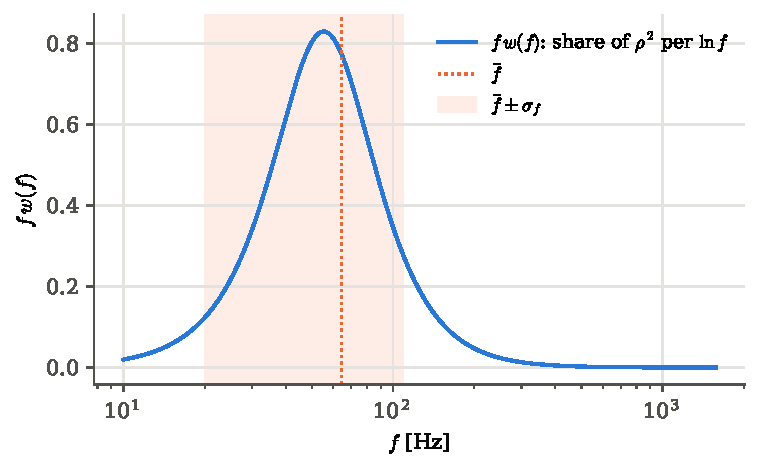
\includegraphics[width=0.7\linewidth]{figures/ch10/cf94_weight.pdf}
\caption{Where a $1.4+1.4\,M_\odot$ inspiral accumulates its signal-to-noise ratio in the advanced-detector noise of
Cutler and Flanagan: $f\,w(f)$ is the share of $\rho^2$ per unit $\ln f$. The weight is a few tens of hertz wide; its
mean (dotted) and spread (band) set the timing errors with and without an unknown phase.}
\label{10b:fig:cf94-weight}
\end{figure}

\paragraph{Example: Cutler and Flanagan's Table I.} The full five-parameter matrix is a test of the whole machinery,
because Cutler and Flanagan published its result for five mass pairs \cite[Table~I]{CutlerFlanagan1994}, normalised
to $\rho=10$. They quote the chirp mass and the reduced mass $\mu=\eta M=\mathcal M\eta^{2/5}$, so we convert our
$(\ln\mathcal M,\ln\eta)$ covariance with the Jacobian of $\ln\mu=\ln\mathcal M+\tfrac25\ln\eta$
(\cref{10a:sec:reparam}). The comparison:

\begin{center}
\footnotesize
\setlength{\tabcolsep}{4pt}
\begin{tabular}{@{}lccccc@{}}
\toprule
$m_1+m_2$ [$M_\odot$] & $\Delta\phi_c$ & $\Delta t_c$ [ms] & $\Delta\mathcal M/\mathcal M$ [\%] & $\Delta\mu/\mu$ [\%] & $c_{\mathcal M\mu}$\\\midrule
$2.0+1.0$ paper / ours & $1.31$ / $\TenBcfPhicA$ & $0.721$ / $\TenBcfTcA$ & $0.0038$ / $\TenBcfMcA$ & $0.39$ / $\TenBcfMuA$ & $0.899$ / $\TenBcfCorrA$\\
$1.4+1.4$ & $1.28$ / $\TenBcfPhicB$ & $0.713$ / $\TenBcfTcB$ & $0.0040$ / $\TenBcfMcB$ & $0.41$ / $\TenBcfMuB$ & $0.906$ / $\TenBcfCorrB$\\
$10+1.4$ & $1.63$ / $\TenBcfPhicC$ & $1.01$ / $\TenBcfTcC$ & $0.020$ / $\TenBcfMcC$ & $0.54$ / $\TenBcfMuC$ & $0.927$ / $\TenBcfCorrC$\\
$15+5$ & $2.02$ / $\TenBcfPhicD$ & $1.44$ / $\TenBcfTcD$ & $0.113$ / $\TenBcfMcD$ & $1.5$ / $\TenBcfMuD$ & $0.954$ / $\TenBcfCorrD$\\
$10+10$ & $1.98$ / $\TenBcfPhicE$ & $1.43$ / $\TenBcfTcE$ & $0.16$ / $\TenBcfMcE$ & $1.9$ / $\TenBcfMuE$ & $0.958$ / $\TenBcfCorrE$\\
\bottomrule
\end{tabular}
\end{center}

\noindent Every entry agrees to within $\TenBcfMaxDev\%$, which is the rounding of the published table and of
their crude ISCO cut-off. Three features are the projection picture at work. The chirp mass is measured a hundred
times better than the reduced mass, because $u^{-5/3}$ dominates the phase at low frequency while the mass ratio
enters only through the smaller 1PN and 1.5PN terms. The two mass errors are strongly correlated
($c_{\mathcal M\mu}>0.9$), because the 1PN signature of $\eta$ is partly imitated by the Newtonian signature of
$\mathcal M$. And all errors grow with the total mass, because a heavier binary leaves the band at a lower ISCO
frequency and spends fewer cycles in it.

Cutler and Flanagan state the noise density $p(n)\propto e^{-(n|n)/2}$, the Fisher matrix and its inverse in three
equations \cite[Sec.~II B]{CutlerFlanagan1994}. Between them lie the variance of a Fourier mode
(\cref{10b:eq:mode-variance}), the density of one realisation (\cref{10b:eq:noise-density}), the expected curvature of
the log-likelihood (\cref{10b:eq:gw-fisher}) and the weighted-average form
(\cref{10b:eq:fisher-blocks}), which turns their table into a statement about projections of phase signatures.

\begin{pitfall}[Normalised tables hide the distance]
Forecast tables are often quoted at a fixed $\rho$ (here $10$; Eda et al.\ use $10$, Barack and Cutler $30$
\cite{BarackCutler2004}). Every Fisher error scales as $1/\rho$, so a table at $\rho=10$ says nothing about whether a
given source reaches $\rho=10$. Always compute $\rho$ for the source at its distance first, then rescale.
\end{pitfall}

\subsection{The Fisher matrix as a distance between waveforms}
\label{10b:sec:metric}

There is a second way to read $\Gamma_{ij}$, and it explains how searches are built. If the true wave has parameters
$\params$ and the template has $\params+\Delta\params$, how much of the signal-to-noise ratio does the template recover?
The \newterm{match} $\mathsf M$ is the normalised overlap
\begin{equation}
  \mathsf M(h,h')=\frac{(h|h')}{\sqrt{(h|h)(h'|h')}}\le1,
\end{equation}
the cosine of the angle between the two waveforms in the space with inner product $(\cdot|\cdot)$; the bound is the
Cauchy--Schwarz inequality, with equality when $h'\propto h$. A filter built with $h'$ and run on a signal $h$ has mean $\mathsf M\rho$ instead of $\rho$ (by
\eqref{10b:eq:z-dist}), so $1-\mathsf M$ is the fractional loss of signal-to-noise ratio. For a small change write the
unit-norm waveform $\hat h=h/\rho$, so that $\mathsf M=(\hat h|\hat h')$. For two unit vectors
$(\hat h-\hat h'|\hat h-\hat h')=2-2\mathsf M$, and for phase parameters (which leave $\rho$ unchanged,
\cref{10b:eq:fisher-blocks}) $\hat h'-\hat h\simeq\Delta\theta^i\,\partial_ih/\rho$. Therefore
\begin{align}
  1-\mathsf M
  &\eqby{1}\tfrac12\big(\hat h'-\hat h\,\big|\,\hat h'-\hat h\big)
   \eqby{2}\frac{1}{2\rho^2}\,\Delta\theta^i\Delta\theta^j\,(\partial_ih|\partial_jh)
   \eqby{3}\frac{\Delta\params\T\Gamma\,\Delta\params}{2\rho^2}.
  \label{10b:eq:match-metric}
\end{align}
\begin{explain}
  \item Expand the square with $(\hat h|\hat h)=(\hat h'|\hat h')=1$.
  \item Insert $\hat h'-\hat h\simeq\Delta\theta^i\partial_ih/\rho$ and use bilinearity.
  \item The definition \eqref{10b:eq:gw-fisher}.
\end{explain}
So $\Gamma_{ij}/\rho^2$ is the \emph{metric} that measures how different two waveforms are, and the Fisher
$1\sigma$ ellipsoid $\Delta\params\T\Gamma\Delta\params=1$ is the set of waveforms with $\rho^2(1-\mathsf M)=\tfrac12$: the
template loses exactly the amount of log-likelihood that defines one standard deviation. A search bank is laid out
by the same metric: the templates are spaced so that the worst match to any possible signal stays above a chosen value
(typically $0.97$), which is why high-$\rho$ errors and bank densities are both set by $\Gamma$.
The script (\pyname{16_whiten_chi2.py}) checks the expansion for a change of the chirp mass alone: for
$\delta\ln\mathcal M=10^{-4}$, $3\times10^{-4}$, $10^{-3}$, $3\times10^{-3}$ the computed $1-\mathsf M$ is
$\TenBmatchA$, $\TenBmatchB$, $\TenBmatchC$, $\TenBmatchD$, against $\TenBmetricA$, $\TenBmetricB$, $\TenBmetricC$ and
$\TenBmetricD$ from \eqref{10b:eq:match-metric} with $\Gamma_{\ln\mathcal M\ln\mathcal M}=\TenBmatchGamma$ (right panel of
\cref{10b:fig:det-chi2}). The two agree to a part in $10^{3}$ for the smallest changes and separate once the phase
has moved by a radian (where the surface of waveforms has curved away from its tangent plane, the content of
\cref{10b:sec:lsa}).
\section{Environments as power laws in the phase}
\label{10b:sec:env}

A binary in vacuum loses energy only to gravitational waves. A binary inside a dark-matter spike, an accretion
disc or a gas cloud loses some more: to the wake that drags behind the companion, to the matter it swallows, to the
torque of the disc. Each of these makes the binary sweep through frequency a little faster, and by
\cref{T2a:eq:psi-derivs} anything that changes the sweep rate changes the Fourier phase. The projection picture of
\cref{10b:fig:projection} tells us that whether LISA can see such a change depends on one thing only: the shape of
the phase change as a function of frequency, and how well the vacuum parameters can imitate it. So the question is:
\begin{center}
\emph{what shape does an environmental energy loss give to the phase, and how does the shape differ from one
environment to the next?}
\end{center}
The answer, derived in \cref{T2a:sec:forces} for dynamical friction and in general form in \cref{T2g:sec:pn}, is that at
leading order every smooth environment adds a single power of frequency, with an exponent fixed by its physics. That
is what turns many separate dark-matter and astrophysics problems into one statistical problem with a single
parameter, the exponent.

\subsection{From an extra power to a power law in the phase}
\label{10b:sec:env-derive}

\emph{What the physics supplies.} The derivation belongs to the theory and is done in \cref{T2a:sec:forces}; here
we recall its result in the form the forecast needs. The orbit is quasi-circular and shrinks slowly
(\cref{T2a:sec:chirp}); the environment removes a power $P_{\rm env}$ on top of the gravitational-wave power
$P_{\rm GW}$, with a small ratio that varies as a power of the radius, $\epsilon\equiv P_{\rm env}/P_{\rm GW}\propto r^p\ll1$.
Energy balance with the vacuum binding energy $E(f)$ of \cref{T2a:eq:Ef} then speeds up the sweep by the factor
$1+\epsilon$ (\cref{T2a:eq:fdot-env}), and Kepler's law $r\propto f^{-2/3}$ turns the power of $r$ into a power of $f$:
\begin{equation}
  \dot f=\dot f_{\rm V}\,(1+\epsilon),
  \qquad
  \epsilon=c_f\,f^{-n},\quad n=\frac{2p}{3},
  \label{10b:eq:fdot-eps}
\end{equation}
where $\dot f_{\rm V}=Kf^{11/3}$, $K=\tfrac{96}5\pi^{8/3}(G\mathcal M/c^3)^{5/3}$, is the vacuum chirp rate
\eqref{T2a:eq:fdot} and $\mathcal M$ the chirp mass. Because the curvature of the Fourier phase is $2\pi/\dot f$
(\cref{T2a:eq:psi-derivs}: the slope of $\Psi$ is the arrival time of each frequency, so a faster sweep bends it),
integrating the change of curvature twice gives the environmental part of the phase (\cref{T2a:eq:ppe}):
\begin{equation}
  \delta\Psi(f)
  =-\frac{2\pi c_f}{K}\,\frac{f^{-n-5/3}}{(n+\frac83)(n+\frac53)}
  \eqby{1}-\frac{2\pi f^2}{\dot f_{\rm V}(f)}\,\frac{\epsilon(f)}{(n+\frac83)(n+\frac53)}
  \eqby{2}\beta\,u^{b},\qquad b=-\frac53-n .
  \label{10b:eq:dpsi-closed}
\end{equation}
\begin{explain}
  \item Rewrite $c_ff^{-n-5/3}/K=f^2\epsilon(f)/\dot f_{\rm V}(f)$.
  \item With the reduced frequency $u=\pi G\mathcal Mf/c^3$ of \eqref{T2g:eq:u}, every power of $f$ is a power of $u$;
        the constants are collected in $\beta$. The two integration constants, $a_0+a_1f$, are a shift of $\phi_c$
        and $t_c$ and are absorbed by those parameters.
\end{explain}
The middle form is the one the analysis uses: it gives the phase shift at any frequency directly from the ratio
$\epsilon$ there. The factor $2\pi f^2/\dot f_{\rm V}$ is $2\pi$ times the number of cycles the binary spends near $f$
(per unit $\ln f$), so in words the phase shift is ``the fractional speed-up times the number of radians spent there,
divided by a number of order ten''. The last form is the \newterm{parametrised post-Einsteinian} (ppE) phase
correction of Yunes and Pretorius \cite[eq.~(1)]{YunesPretorius2009}: $\beta$ carries the strength of the effect and
$b$ its physics (\cref{T2g:eq:ppe-rule}, where the same rule is derived for any correction that scales as a power of
the orbital speed). In post-Newtonian language, the expansion in powers of $(v/c)^2$ of \cref{T2g:sec:pn}, a relative
correction $\epsilon\propto f^{-n}=(v/c)^{-3n}$ enters at order $-\tfrac32n$\,PN.

\subsection{The exponents of the common environments}
\label{10b:sec:env-exponents}

Each exponent follows from how $P_{\rm env}/P_{\rm GW}$ scales with $r$, and $P_{\rm GW}=\tfrac{32}5G^4M^3\mu^2/(c^5r^5)$
(the quadrupole power of a circular binary, \cref{T2g:eq:power-binary})
falls as $r^{-5}$, steeper than almost anything an environment does. That is why environments matter at large radius,
at the low-frequency start of the band.

\paragraph{Dynamical friction in a spike.} Chandrasekhar's drag in a density $\rho\propto r^{-\gamma}$ removes
$P_{\rm DF}=4\pi G^2m_2^2\rho\ln\Lambda/v$ with $v=\sqrt{GM/r}$ (\cref{T2a:eq:df}). Divided by $P_{\rm GW}\propto r^{-5}$
this is $\propto\rho\,r^{11/2}\propto r^{11/2-\gamma}$, with the constants worked out in \cref{T2a:eq:eps}
\cite[eq.~(16)]{Eda2015}, \cite[eq.~(16)]{Speeney2022}. So
\[
  p=\tfrac{11}2-\gamma,\qquad n=\tfrac{11-2\gamma}{3},\qquad b=\tfrac{2\gamma-16}{3}.
\]
For the adiabatic spike $\gamma=7/3$ this is $b=-34/9\approx-3.78$, a $-3.2$PN effect.

\paragraph{Gas accretion onto the central black hole.} Suppose the heavy hole grows at a fraction $f_{\rm Edd}$ of the
Eddington rate, $\dot M/M=f_{\rm Edd}/t_{\rm S}$ with the Salpeter time $t_{\rm S}\approx4.5\times10^7$\,yr. The
companion feels a slowly growing central mass. Its specific angular momentum $\sqrt{GMr}$ is conserved (the force is
still central), so $r\propto1/M$, and Kepler's law $\omega^2=GM/r^3$ gives $\omega\propto M^2$, hence
$\dot f/f=2\dot M/M$ in addition to the radiative sweep. The fractional speed-up is
\begin{equation*}
  \epsilon=\frac{2f\,\dot M/M}{\dot f_{\rm V}}\propto\frac{f}{f^{11/3}}=f^{-8/3},
  \qquad n=\tfrac83,\quad b=-\tfrac{13}3 ,
\end{equation*}
a $-4$PN effect, as for the mass changes discussed by Barausse et al.\ \cite[Sec.~XII]{Barausse2014}.

\paragraph{Migration in a thin disc.} A companion embedded in a thin accretion disc exchanges angular momentum with
it. For type-I migration far from the inner edge, Barausse et al.\ find
$\dot L_{\rm migr}/\dot L_{\rm GW}=10^{-5}f_{\rm Edd}^{2/5}(M/10^6M_\odot)^{7/5}(\alpha/0.1)^{-3/5}\tilde r^{7/2}$, with
$\tilde r=rc^2/(GM)$ and $\alpha$ the disc viscosity parameter \cite[eq.~(108)]{Barausse2014}. On a circular orbit
$\dot E=\omega\dot L$ for both torques, so the energy ratio is the same and $p=7/2$, $n=7/3$, $b=-4$.

\begin{table}[htbp]
\centering
\small
\renewcommand{\arraystretch}{1.2}
\begin{tabular}{@{}lccc@{}}
\toprule
effect & $\epsilon=P_{\rm env}/P_{\rm GW}\propto$ & $b=-\frac53-n$ & PN order\\\midrule
friction, spike $\rho\propto r^{-\gamma}$ \cite{Eda2015,Coogan2022} & $r^{11/2-\gamma}$ & $\frac{2\gamma-16}3$ ($-3.78$ at $\frac73$) & $\gamma-\frac{11}2$\\
friction, uniform medium & $r^{11/2}$ & $-\frac{16}3$ & $-5.5$\\
collisionless accretion, spike \cite{Barausse2014} & $r^{9/2-\gamma}$ & $\frac{2\gamma-14}3$ & $\gamma-\frac92$\\
enclosed dark-matter mass (no loss) \cite{Eda2015,Speeney2022} & $r^{3-\gamma}$ & $\frac{2\gamma-11}3$ & $\gamma-3$\\
Eddington accretion onto $m_1$ & $f^{-8/3}$ & $-\frac{13}3$ & $-4$\\
type-I migration, thin disc \cite{Barausse2014} & $r^{7/2}$ & $-4$ & $-3.5$\\
dipole radiation (Brans--Dicke) \cite{YunesPretorius2009} & $r$ & $-\frac73$ & $-1$\\
massive graviton (propagation) \cite{YunesPretorius2009} & --- & $-1$ & $+1$\\\midrule
GR: chirp mass, 1PN, 1.5PN, $\phi_c$, $t_c$ & --- & $-\frac53,\ -1,\ -\frac23,\ 0,\ 1$ & \\
vector ultralight dark matter \cite{Chase2025} & \multicolumn{3}{l}{a step at a resonance: not a power law}\\
\bottomrule
\end{tabular}
\caption{Leading-order exponents of environmental and beyond-GR phase corrections $\delta\Psi=\beta u^b$. The PN
order of a relative correction $\epsilon\propto f^{-n}$ is $-\frac32n$. The GR exponents in the last block are the
signatures every environmental term must be distinguished from.}
\label{10b:tab:exponents}
\end{table}

\Cref{10b:tab:exponents} collects these. All the dissipative environments sit at $b\lesssim-3$, well below the
chirp-mass exponent $-5/3$; the propagation and dipole corrections of modified gravity sit between $-7/3$ and $-1$,
in the middle of the GR terms. \Cref{10b:fig:signatures} shows what that means on the frequency axis.

\begin{figure}[htbp]
\centering
\begin{tikzpicture}
\begin{axis}[width=0.62\linewidth,height=5.4cm,ymode=log,xmin=0,xmax=1.7,ymin=1e-7,ymax=50,
  xlabel={$\log_{10}(f/f_{\rm lo})$},ylabel={$|g(f)|/|g(f_{\rm lo})|$},
  legend style={font=\scriptsize,draw=none,fill=none,at={(1.02,0.5)},anchor=west},legend cell align=left,
  tick label style={font=\footnotesize},label style={font=\small}]
  \addplot[domain=0:1.7,samples=2,thick,black] {10^(-5/3*x)};
  \addplot[domain=0:1.7,samples=2,thick,black,dashed] {10^(1*x)};
  \addplot[domain=0:1.7,samples=2,thick,black,dotted] {1};
  \addplot[domain=0:1.7,samples=2,thick,formblue] {10^(-34/9*x)};
  \addplot[domain=0:1.7,samples=2,thick,fibreorange] {10^(-13/3*x)};
  \addplot[domain=0:1.7,samples=2,thick,tangentgreen] {10^(-7/3*x)};
  \legend{$\mathcal M$: $u^{-5/3}$, $t_c$: $u^{1}$, $\phi_c$: $u^0$, friction $\gamma=\frac73$: $u^{-34/9}$,
          Eddington accretion: $u^{-13/3}$, dipole: $u^{-7/3}$}
\end{axis}
\end{tikzpicture}
\caption{Phase signatures over the LISA band of the benchmark binary (a factor $50$ in frequency), normalised at the
start frequency $f_{\rm lo}$. On these axes each is a straight line of slope $b$. The environmental signatures fall
far more steeply than the chirp-mass one and are concentrated in the first fraction of a decade; a dipole term lies
close to the chirp-mass line and is easily imitated by it.}
\label{10b:fig:signatures}
\end{figure}

\subsection{Example: how large is each effect for one source?}
\label{10b:sec:env-example}

Take the benchmark of \cref{T2a:sec:chirp} that recurs below: a $10^3+1.4\,M_\odot$ intermediate mass-ratio inspiral
observed for the last five years before its ISCO (the innermost stable circular orbit, where the inspiral ends,
\cref{T2a:eq:fisco}), from $f_{\rm lo}=\TenBenvflo$\,mHz up to $1$\,Hz (its ISCO is at
$\TenBenvfisco$\,Hz, above the LISA band), chirp mass $\TenBenvMc\,M_\odot$. The script \pyname{10_env_phases.py}
evaluates $\epsilon(f)$ for each effect with the parameters of the literature (the spike density
$\rho_6=5.45\times10^{15}M_\odot\,{\rm pc}^{-3}$ at $10^{-6}$\,pc of Coogan et al.\ \cite{Coogan2022}, $\xi=0.58$,
$\ln\Lambda=\ln\sqrt{m_1/m_2}$; $f_{\rm Edd}=1$ for gas accretion; $f_{\rm Edd}=0.1$, $\alpha=0.1$ for the disc) and
converts it to $\delta\Psi$ with \eqref{10b:eq:dpsi-closed}. At the start of the band:

\begin{center}
\small
\begin{tabular}{@{}lccc@{}}
\toprule
effect & $b$ & $\epsilon(f_{\rm lo})$ & $|\delta\Psi(f_{\rm lo})|$ [rad]\\\midrule
friction, spike $\gamma=7/3$ & $\TenBenvBDfA$ & $\TenBenvEpsDfA$ & $\TenBenvDpsiDfA$\\
friction, spike $\gamma=3/2$ & $\TenBenvBDfB$ & $\TenBenvEpsDfB$ & $\TenBenvDpsiDfB$\\
collisionless accretion, $\gamma=7/3$ & $\TenBenvBAcc$ & $\TenBenvEpsAcc$ & $\TenBenvDpsiAcc$\\
enclosed mass, $\gamma=7/3$ (order of magnitude) & $\TenBenvBPull$ & $\TenBenvEpsPull$ & $\TenBenvDpsiPull$\\
Eddington gas accretion onto $m_1$ & $\TenBenvBEdd$ & $\TenBenvEpsEdd$ & $\TenBenvDpsiEdd$\\
type-I migration, thin disc & $\TenBenvBMig$ & $\TenBenvEpsMig$ & $\TenBenvDpsiMig$\\
\bottomrule
\end{tabular}
\end{center}

\noindent A tiny $\epsilon$ can still give a large phase shift, because $2\pi f^2/\dot f_{\rm V}$ is enormous for a
binary that spends years near $f_{\rm lo}$: an Eddington-limited growth that changes the sweep rate by six parts in
ten million still shifts the phase by more than a radian. Before trusting the closed form, the script compares it
with the exact double integral of $2\pi/\dot f-2\pi/\dot f_{\rm V}$ for a weak spike; after removing the
$a_0+a_1f$ that $t_c$ and $\phi_c$ absorb, they differ by $\TenBenvClosedErr$ of the shift.

\Cref{10b:fig:env-phases} shows the whole band. One number in the table is a warning: for the static $7/3$ spike,
$\epsilon(f_{\rm lo})=\TenBenvEpsDfA$, because friction equals radiation at $f_{\rm eq}=\TenBenvfeq$\,mHz, just below
the band (\cref{T2a:sec:forces}). There the expansion in $\epsilon$ is not valid, and the full dephasing
\cref{T2a:eq:hyp} must be used. The power law is a statement about weak environments, which are precisely the ones
whose detectability is in question.

\begin{figure}[htbp]
\centering
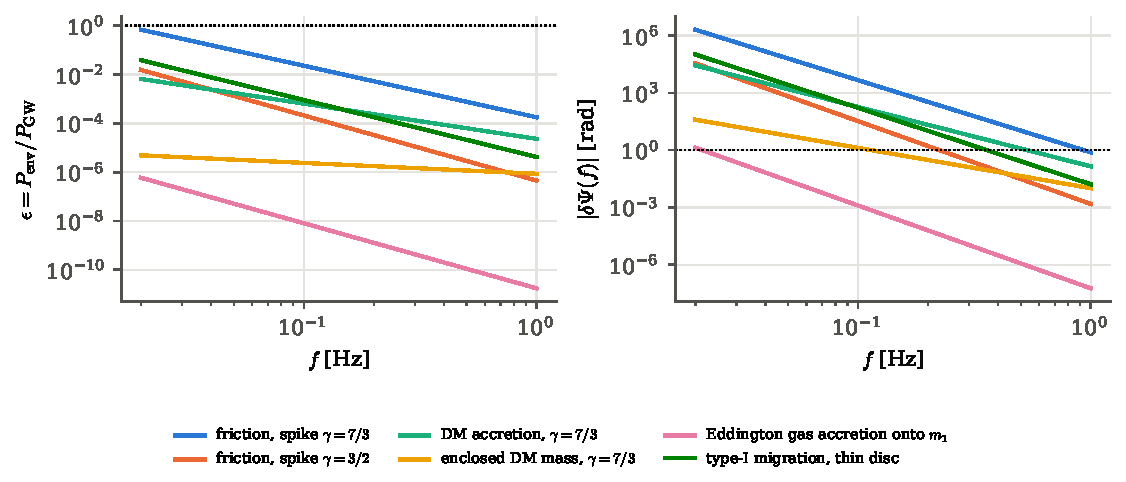
\includegraphics[width=\linewidth]{figures/ch10/env_phases.pdf}
\caption{The six effects for the $10^3+1.4\,M_\odot$ binary over its last five years in the LISA band. Left: the
ratio $\epsilon$ of environmental to gravitational-wave power; each is a power law falling towards high frequency.
Right: the resulting Fourier-phase shift \eqref{10b:eq:dpsi-closed}; the dotted line marks one radian. All shifts are
largest at the start of the band.}
\label{10b:fig:env-phases}
\end{figure}

\paragraph{The hidden assumption, and a counterexample.} ``An environment is a power law in the phase'' contains an
assumption: that the environment changes smoothly and monotonically with radius, so a single power of $r$ describes
it across the band. A vector ultralight dark-matter field breaks it. Its oscillating potential does nothing on average
until the orbital frequency crosses a resonance with the field, and then shifts the orbit within a narrow band
\cite{Chase2025}. Chase, L\'opez Nacir and Yunes find that the resulting phase correction is a step, and that below the
threshold it is partly degenerate with $t_c$ and $\phi_c$. In the projection picture this is no surprise: a correction
of the form $a_0+a_1f$ lies entirely in the span of the $\phi_c$ and $t_c$ signatures, $g_\perp=0$, and it is invisible
however large it is. Only the sudden switch-on, which no smooth GR term can imitate, can be measured. So the lesson in
one line: \emph{a phase correction is measured by its shape, not its size}.
\section{One forecast for every environment}
\label{10b:sec:forecast}

The two previous sections give us all the pieces. \Cref{10b:sec:fisher} says that a phase parameter is measured by
the part of its signature that the vacuum parameters cannot imitate, and \cref{10b:sec:env} says that the signature of
any smooth environment is a single power, $\delta\Psi=\beta u^b$, with an exponent set by its physics: the ppE form of
\cref{T2g:eq:ppe-rule}, with $u=\pi G\mathcal Mf/c^3$ the reduced frequency, $\beta$ the strength and $b$ the exponent. So instead of
writing one forecast for dark-matter friction, another for accretion and another for a gas disc, we can ask a single
question for a given source:
\begin{center}
\emph{for each exponent $b$, what is the smallest amplitude $\beta$ that LISA would detect?}
\end{center}
One Fisher matrix per value of $b$ answers it, and the answer is one curve. Every environment then becomes a point,
above or below the curve. We build that curve for the benchmark intermediate mass-ratio inspiral and read it.

\subsection{The noise curve, checked against its source}
\label{10b:sec:robson}

The forecast weights each frequency by $1/S_n(f)$, the one-sided noise spectrum of \cref{10b:sec:noise-fd}, so the noise
model comes first. We use the sky-averaged LISA
sensitivity of Robson, Cornish and Liu \cite[eqs.~(10)--(14)]{Robson2019}: optical metrology and test-mass acceleration
noise, divided by the sky-averaged response of two Michelson channels (the factor $\tfrac3{10}$ of
\cref{T2g:eq:sixty}: how strongly a source at a random place on the sky registers), plus the Galactic confusion noise for a
four-year mission. Its pieces are derived and explained in \cref{T2a:sec:lisa}; the formula is \cref{T2a:eq:Sn}. The
script \pyname{11_lisa_robson.py} implements it independently of chapter~T2 (the two agree to
$\TenBrobTtwoDiff$) and checks it against what the paper itself shows and computes.

\paragraph{Their figure.} The script renders page~6 of the paper, finds the frame of Figure~4, calibrates its axes and
reads the curve of $\sqrt{S_n}$ from the colour of its pixels. \Cref{10b:fig:robson} overlays the digitised points on our
curve. Below $30$\,mHz they agree to within $\TenBrobDevLow\%$, the precision of reading a plotted line; at
$f=1$, $10$ and $100$\,mHz the ratios ours/theirs are $\TenBrobOursC/\TenBrobReadC$,
$\TenBrobOursE/\TenBrobReadE$ and $\TenBrobOursG/\TenBrobReadG$. The last is $15\%$ high: above the transfer frequency
$f_*=c/(2\pi L)=\TenBrobFstar$\,mHz (their $19.09$\,mHz), where the wave's phase advances by a radian while light
crosses one arm, so the arm starts to average the wave away (\cref{T2g:eq:transfer}), their plot uses the exact numerical response, which oscillates,
while the formula uses the smooth fit $R(f)=\tfrac3{10}/[1+0.6(f/f_*)^2]$ of their eq.~(9). The wiggles are visible
in the digitised points; the fit runs through their average.

\begin{figure}[htbp]
\centering
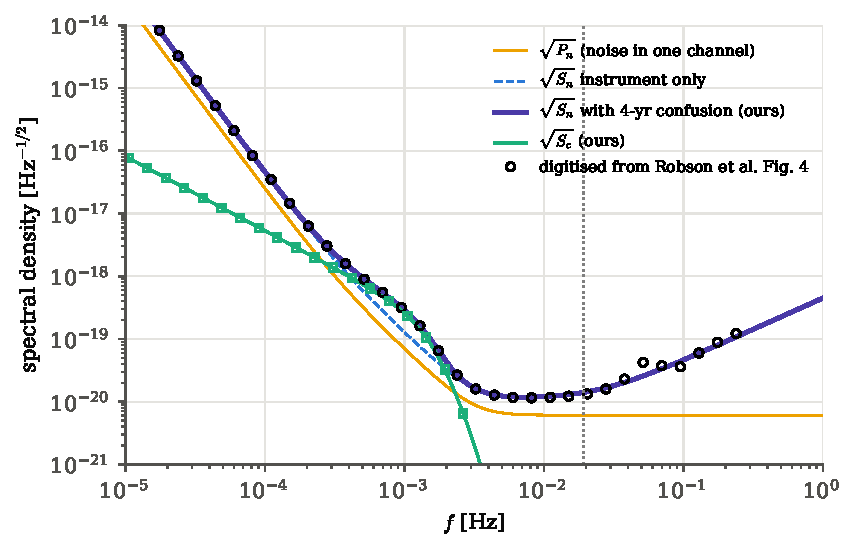
\includegraphics[width=0.78\linewidth]{figures/ch10/robson_curve.pdf}
\caption{The LISA sensitivity used in all forecasts, against Figure~4 of Robson, Cornish and Liu digitised from the
published PDF (open circles: $\sqrt{S_n}$; open squares: the Galactic confusion noise $\sqrt{S_c}$). The thick curve
includes four years of confusion noise; the thin dashed one is the instrument alone. Above the transfer frequency
(dotted) the published curve shows the oscillations of the exact detector response, which the fit smooths.}
\label{10b:fig:robson}
\end{figure}

\paragraph{Their worked numbers.} Robson et al.\ quote three numbers that test both the curve and the signal
normalisation.
\begin{itemize}[itemsep=2pt,leftmargin=1.2em]
  \item \emph{A verification binary.} SDSS J0651+2844 ($0.5+0.25\,M_\odot$, $D_L\approx1$\,kpc, $f=2.6$\,mHz) barely
        changes frequency in four years, so its signal-to-noise integral collapses to one frequency. With the
        stationary-phase amplitude $|\tilde h|=\tfrac12A_t\dot f^{-1/2}$ (\cref{T2a:eq:spa}) and the band
        $\Delta f=\dot fT$ swept in a time $T$,
        \begin{align*}
          \rho^2
          \eqby{1}\frac{16}5\int\frac{|\tilde h|^2}{S_n}\dd f
          \eqby{2}\frac{16}{5}\,\frac{A_t^2T}{4S_n(f)}
          \eqby{3}\frac{h_{\rm GB}^2}{S_n(f)},\qquad
          h_{\rm GB}=\frac{8\,T^{1/2}(G\mathcal M/c^3)^{5/3}\pi^{2/3}f^{2/3}}{5^{1/2}D_L/c},
        \end{align*}
        \begin{explain}
          \item Sky-, polarisation- and inclination-averaged signal-to-noise ratio (\cref{T2a:eq:snr}; the $\tfrac45$ in
                $\tfrac{16}5=4\cdot\tfrac45$ is the inclination average \eqref{T2g:eq:four-fifths}), with
                $|\tilde h|$ the face-on stationary-phase amplitude.
          \item $\int|\tilde h|^2\dd f=\tfrac14A_t^2\int\dd f/\dot f=\tfrac14A_t^2T$, the amplitude and $S_n$ being constant
                over the tiny band.
          \item $A_t=4(G\mathcal M)^{5/3}(\pi f)^{2/3}/(c^4D_L)$, so $\frac{16}{5}\cdot\frac{16}{4}=\frac{64}{5}$ and
                $\sqrt{64/5}=8/\sqrt5$: their eq.~(27).
        \end{explain}
        We obtain $\rho=\TenBrobJsnr$; they quote $140$. (Without the confusion noise it would be $\TenBrobJsnrNoConf$:
        at $2.6$\,mHz the unresolved Galaxy matters.) Our $h_{\rm GB}=\TenBrobJhGB$\,Hz$^{-1/2}$ is $10\%$ above the
        $2.8\times10^{-18}$ they print, although the signal-to-noise ratios agree; the printed amplitude is
        inconsistent with their own $\rho=140$ and is presumably rounded from slightly different inputs.
  \item \emph{A GW150914-like binary} five years before merger sweeps from $16$ to $29$\,mHz during four years; we find
        $\TenBrobGWfFive$ and $\TenBrobGWfOne$\,mHz (\cref{T2a:sec:chirp} derives it by hand).
  \item \emph{An equal-mass $10^6M_\odot$ binary at $z=3$} radiates at $2.93\times10^{-5}$\,Hz one year before merger when
        the detector-frame mass $(1+z)M$ is used; we find $\TenBrobBigf$\,Hz.
\end{itemize}

\subsection{The benchmark source and its vacuum errors}
\label{10b:sec:benchmark}

The source is the $10^3+1.4\,M_\odot$ binary of \cref{10b:sec:env-example} at $D_L=76$\,Mpc, the distance of the
astrophysical benchmark of Coogan et al.\ \cite{Coogan2022}. LISA observes its last five years before the ISCO (\cref{T2a:eq:fisco}),
from $f_{\rm lo}=\TenBppflo$\,mHz to the $1$\,Hz edge of the band, and the sky-averaged signal-to-noise ratio is
$\rho=\TenBppSNR$. The parameters are those of \cref{10b:sec:signal-model} (chirp mass, mass ratio, coalescence time $t_c$ and phase
$\phi_c$, amplitude; their physical meaning is listed in \cref{T2g:tab:symbols}) plus the environmental amplitude,
\begin{equation}
  \params=(\ln\mathcal M,\ \ln\eta,\ t_c,\ \phi_c,\ \ln\mathcal A,\ \beta),\qquad
  \Psi=\Psi_{\rm 1.5PN}+\beta u^b,
  \label{10b:eq:theta6}
\end{equation}
with $\Psi_{\rm 1.5PN}$ the phase \eqref{10b:eq:psi-pn} through 1.5 post-Newtonian order (\cref{T2g:sec:pn}),
evaluated at the vacuum, $\beta=0$: the question is whether the data could tell an environment apart from no
environment. Without the environmental term, the five-parameter errors are $\sigma_{\ln\mathcal M}=\TenBppGRlnMc$,
$\sigma_{\ln\eta}=\TenBppGRlneta$, $\sigma_{t_c}=\TenBppGRtc$\,s, $\sigma_{\phi_c}=\TenBppGRphic$\,rad and
$\sigma_{\ln\mathcal A}=\TenBppGRlnA=1/\rho$. The chirp mass is fixed to a few parts in ten million because the binary
completes about a million cycles in the band; this is the reservoir of precision an environment can draw on.

\subsection{The error on \texorpdfstring{$\beta$}{beta} as a function of the exponent}
\label{10b:sec:sigma-b}

The script \pyname{12_ppe_scan.py} computes the six-parameter Fisher matrix for $815$ values of $b$ between $-6.5$ and
$1.6$:

\pyfile[firstline=48,lastline=57,firstnumber=48]{code/ch10/12_ppe_scan.py}{One Fisher matrix per exponent}

\noindent Line 49 is \eqref{10b:eq:gw-fisher} with the extra row $\partial\ln\tilde h/\partial\beta=-iu^b$. Line 52 records
both the marginalised error and the error with all other parameters known, $1/\sqrt{\Gamma_{\beta\beta}}$. Line 53 turns
$\sigma_\beta$ into a phase: a $3\sigma$ shift at the start of the band. The lines that follow redo the calculation in the
projection form \eqref{10b:eq:sigma-residual}, fitting $u^b$ with the vacuum signatures by weighted least squares; the
two agree to $\TenBppSchurCheck$.

Because $\beta$ multiplies a different power of $u$ for each $b$, its value is not comparable across $b$. A physical
measure is the phase shift it produces where it is largest, $\sigma_\beta u_{\rm lo}^{\,b}$ at $f_{\rm lo}$.
\Cref{10b:fig:ppe-sigma} shows it.

\begin{figure}[htbp]
\centering
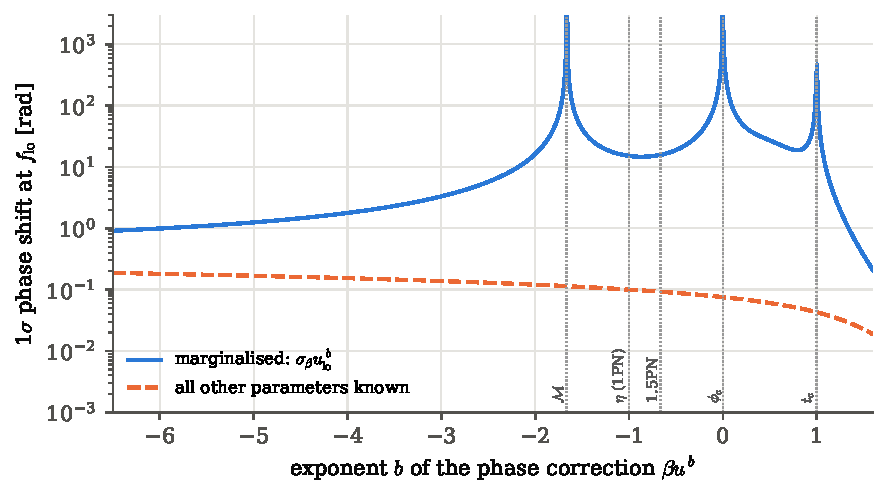
\includegraphics[width=0.8\linewidth]{figures/ch10/ppe_sigma.pdf}
\caption{The $1\sigma$ error of a power-law phase correction, expressed as the phase shift it allows at the start of the
band, for the benchmark binary ($\rho=\TenBppSNR$). Solid: marginalised over $\ln\mathcal M$, $\ln\eta$, $t_c$, $\phi_c$
and $\ln\mathcal A$. Dashed: with all of them known. The marginalised error diverges where $u^b$ coincides with a vacuum
signature: the chirp mass ($b=-5/3$), the phase ($b=0$) and the arrival time ($b=1$).}
\label{10b:fig:ppe-sigma}
\end{figure}

Three things are visible. First, the error diverges at $b=-5/3$, $0$ and $1$, where $u^b$ is exactly the signature of
$\ln\mathcal M$, $\phi_c$ or $t_c$: there $g_\perp=0$ and the correction is simply reabsorbed into a wrong chirp mass,
phase or arrival time. Second, near the 1PN and 1.5PN exponents ($-1$, $-2/3$) the error is large but finite: those
terms are tied to $\eta$ with fixed coefficients, so $\eta$ can imitate only one combination of them. Third, the
marginalised error is far larger than the conditional one even away from the singular points: by a factor
$\TenBppRatioFour$ at $b=-4$, $\TenBppRatioBd$ at the dipole exponent $-7/3$ and $\TenBppRatioMg$ at the massive-graviton
exponent $-1$. A forecast that holds the masses fixed would be wrong by these factors.

\subsection{Correlations: why low-frequency effects separate from the chirp mass}
\label{10b:sec:corr}

The correlation coefficient between two parameters is, in the projection picture, the cosine of the angle between their
signatures (after removing the others). For $\beta$ and $\ln\mathcal M$ alone it is
$\langle u^bu^{-5/3}\rangle_w/\sqrt{\langle u^{2b}\rangle_w\langle u^{-10/3}\rangle_w}$, and the Cauchy--Schwarz inequality
says this is one only if the two functions are proportional over the band. Two decreasing powers look more and more
alike as their exponents approach each other, and more and more different as they separate. An effect with $b\ll-5/3$
is concentrated in the first fraction of a decade above $f_{\rm lo}$ (\cref{10b:fig:signatures}), while the chirp-mass
signature is spread over the whole band. That is why low-frequency effects decorrelate from the chirp mass.

The script shows it directly (\cref{10b:fig:ppe-corr}). With $\eta$ known, the correlation of $\beta$ with
$\ln\mathcal M$ is $\TenBppcMcfixTwo$ at $b=-2$, $\TenBppcMcfixFour$ at $b=-4$ and $\TenBppcMcfixEight$ at $b=-8$. With
$\eta$ free, the picture changes in an instructive way: $\eta$ is now the parameter whose signature is closest to the
environmental one (its correlation with $\beta$ is $\TenBppcetaFour$ at $b=-4$), and the correlation with the chirp mass
drops to $\TenBppcMcFour$. The arrival time, whose signature $2\pi f$ grows with frequency, is the least similar of all,
with a correlation near $\TenBppctcFour$ for every steep effect. Across the singular points the correlations jump
between $\pm1$: on one side $u^b$ is slightly steeper than $u^{-5/3}$, on the other slightly flatter, and the sign of
the compensating chirp-mass error flips.

\begin{figure}[htbp]
\centering
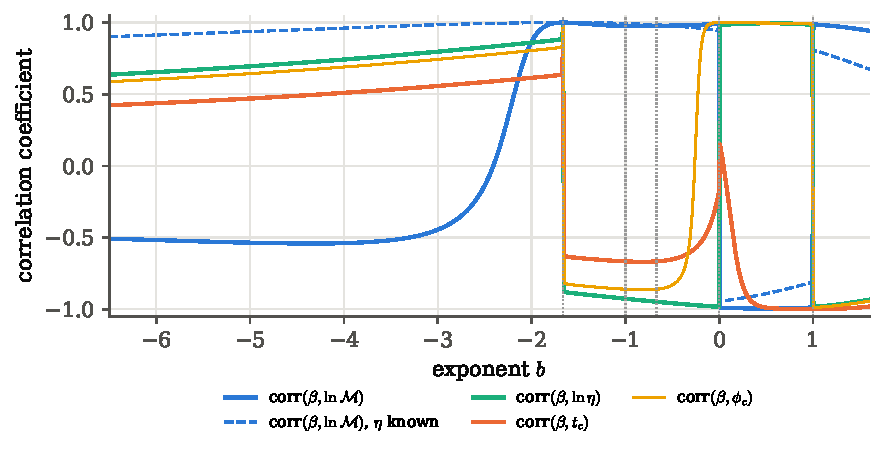
\includegraphics[width=0.8\linewidth]{figures/ch10/ppe_corr.pdf}
\caption{Correlation of the environmental amplitude $\beta$ with the vacuum parameters as a function of the exponent.
Dashed: with $\ln\mathcal M$ when $\eta$ is known, which falls steadily as $b$ moves below $-5/3$. Solid: all parameters
free; $\eta$ then takes over part of the chirp-mass role. Dotted verticals mark the GR exponents.}
\label{10b:fig:ppe-corr}
\end{figure}

\subsection{The detectability map}
\label{10b:sec:map}

Now the single curve. An environment with exponent $b$ and amplitude $\beta$ is detected at $3\sigma$ if
$|\beta|>3\sigma_\beta(b)$, that is if the phase shift it produces at the start of the band exceeds
\begin{equation}
  \delta\Psi_{\rm det}(b)=3\,\sigma_\beta(b)\,u_{\rm lo}^{\,b} .
  \label{10b:eq:map}
\end{equation}
The predicted shift of each physical effect at $f_{\rm lo}$ is the last column of the table in
\cref{10b:sec:env-example}. \Cref{10b:fig:ppe-map} puts them together.

\begin{figure}[htbp]
\centering
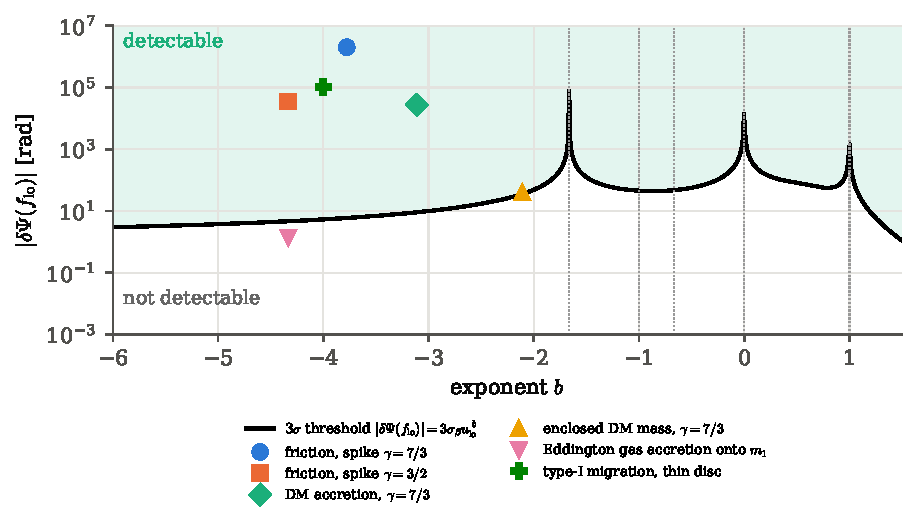
\includegraphics[width=0.85\linewidth]{figures/ch10/ppe_map.pdf}
\caption{Detectability map for the $10^3+1.4\,M_\odot$ binary at $76$\,Mpc ($\rho=\TenBppSNR$). The black curve is the
phase shift at the start of the band that LISA would detect at $3\sigma$, for every exponent $b$; the shaded region above
it is detectable. Points are the effects of \cref{10b:sec:env-example} at their exponents. Everything above the curve is
seen; the curve moves down in proportion to $1/\rho$ for closer sources.}
\label{10b:fig:ppe-map}
\end{figure}

Reading the map, in units of the forecast error $\sigma_\beta$ for each predicted amplitude:
\begin{itemize}[itemsep=1pt,leftmargin=1.2em]
  \item friction in a static $\gamma=7/3$ spike: $\TenBppSigDfA\,\sigma$; in a $\gamma=3/2$ spike: $\TenBppSigDfB\,\sigma$;
  \item collisionless accretion in the $7/3$ spike: $\TenBppSigAcc\,\sigma$;
  \item type-I migration in a thin disc: $\TenBppSigMig\,\sigma$;
  \item the pull of the enclosed dark matter: $\TenBppSigPull\,\sigma$, marginal;
  \item Eddington-limited gas accretion onto the heavy hole: $\TenBppSigEdd\,\sigma$, not detected.
\end{itemize}
The dissipative dark-matter and disc effects are not just detectable, they dominate the phase; the problem for them is
modelling, not detection (\cref{10b:sec:reproduce} shows how much the model matters). The two weak effects sit near the
curve, where the forecast decides.

\paragraph{The same curve in physical units.} For friction, $\beta$ is proportional to the spike density as long as
$\epsilon\ll1$, so the curve converts into a smallest detectable density. \Cref{10b:fig:ppe-rhomin} shows it as a
function of distance (the threshold grows in proportion to $D_L$, because $\rho\propto1/D_L$). At $76$\,Mpc LISA would
see friction from a $\gamma=7/3$ spike with $\rho_6$ as low as $\TenBppRhoMinC\,M_\odot\,{\rm pc}^{-3}$ at
$10^{-6}$\,pc, five orders of magnitude below the static benchmark; for $\gamma=2$ and $3/2$ the thresholds are
$\TenBppRhoMinB$ and $\TenBppRhoMinA$. Above the dotted lines, friction exceeds radiation already at $f_{\rm lo}$
($\rho_6>\TenBppRhoEqC$ for $\gamma=7/3$) and the power-law forecast is not applicable; the benchmark density sits just
below that line.

\begin{figure}[htbp]
\centering
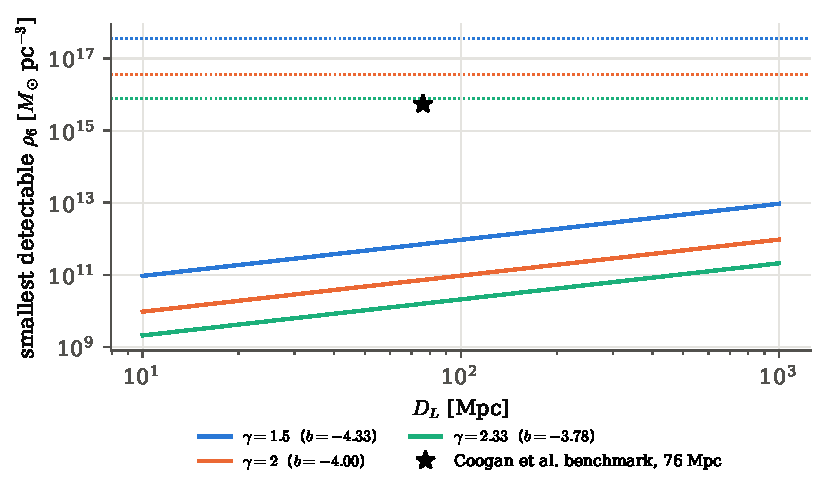
\includegraphics[width=0.75\linewidth]{figures/ch10/ppe_rhomin.pdf}
\caption{Smallest spike density at $10^{-6}$\,pc whose dynamical friction LISA would detect at $3\sigma$ in this binary,
against luminosity distance, for three spike slopes. Dotted: the density at which friction equals radiation at the start
of the band, above which the small-$\epsilon$ expansion fails. The star is the astrophysical benchmark of Coogan et al.}
\label{10b:fig:ppe-rhomin}
\end{figure}

\begin{keyidea}[When is an environment detectable?]
Write the environment as $\delta\Psi=\beta u^b$. Fit it with the vacuum parameters by weighted least squares over the
band, weight $w\propto|\tilde h|^2/S_n$. It is detected at $k\sigma$ when the weighted root-mean-square of the residual
phase exceeds $k/\rho$ radians. The rule ``a dephasing of more than a radian is detectable'' \cite{Speeney2022} keeps the
radian but forgets both the $1/\rho$ and the part that the masses, arrival time and phase can absorb.
\end{keyidea}

\paragraph{How the error scales with the signal strength.} In the Fisher approximation every error scales exactly as
$1/\rho$: double the distance and the curve rises by two. Whether that scaling holds at the signal-to-noise ratios of
real sources is a separate question, answered in \cref{10b:sec:validity} by comparing with a Markov chain.
\section{Reproducing the published forecasts}
\label{10b:sec:reproduce}

A forecast printed in a paper is a claim: ``with this source, this detector and this model, the spike slope would be
measured to a part in a million''. We can trust such a claim only if we can make it again ourselves, with our own
code, and land on the same number, or explain why we do not. Two of the claims already passed: the LISA noise curve
and its worked examples (\cref{10b:sec:robson}) and Cutler and Flanagan's table of errors
(\cref{10b:sec:fisher-examples}). Here are the two dark-matter forecasts on which most of the later literature
builds. Eda, Itoh, Kuroyanagi and Silk \cite{Eda2015} put an intermediate-mass black hole inside a static
dark-matter spike and asked how well an eLISA-like detector would measure the spike. Kim, Lenoci, Stomberg and Xue
\cite{Kim2023} repeated the question for wave-like (ultralight) dark matter, with LISA, a halo that loses its inner
modes to the black hole, and a full Bayesian posterior.

The procedure is the same for both. First derive the quantity the paper plots, from what is already established.
Then rebuild the paper's model, ingredient by ingredient, and compute the same quantity. Then compare, number by
number, and when the two disagree, ask what could have produced the disagreement before deciding.

\subsection{The two phases that papers plot}
\label{10b:sec:two-phases}

Both papers summarise the effect of the dark matter by a ``phase difference'' accumulated between a frequency $f$
and the end of the inspiral. They do not mean the same phase. One is the phase of the Fourier transform, the
quantity that enters the likelihood. The other is the phase of the wave in time, which counts cycles. Both follow
from the stationary-phase formula of \cref{T2a:sec:spa}, so we derive both once.

\emph{Inputs.} The Fourier phase is $\Psi(f)=2\pi ft(f)-\phi(t(f))-\pi/4$ (\cref{T2a:eq:spa}; in words, the Fourier
component at $f$ is built by the short stretch of the chirp that passes through $f$), where $t(f)$ is the
time at which the chirp passes through frequency $f$ and $\phi(t)$ is the phase of the wave in time, with
$\dd\phi/\dd t=2\pi f$. The sweep rate $\dot f(f)$ is whatever the physics gives: vacuum (\cref{T2a:eq:fdot}, set by the chirp mass
$\mathcal M$), or vacuum plus friction (\cref{T2a:eq:fdot-env}).
Let the signal end at $f_I$ (the ISCO, \cref{T2a:eq:fisco}) at the time $t_c$ with the phase $\phi_c$ (the coalescence
constants of \cref{T2g:sec:tc-phic}). Then
\begin{align}
  t(f)&\eqby{1}t_c-\int_f^{f_I}\frac{\dd f'}{\dot f(f')},\qquad
  \phi(t(f))\eqby{2}\phi_c-2\pi\int_f^{f_I}\frac{f'\,\dd f'}{\dot f(f')},\nonumber\\
  \Psi(f)&\eqby{3}2\pi ft_c-\phi_c-\frac\pi4+2\pi\int_f^{f_I}\frac{f'-f}{\dot f(f')}\,\dd f'
  \equiv2\pi ft_c-\phi_c-\frac\pi4+\tilde\Phi(f).
  \label{10b:eq:phitilde}
\end{align}
\begin{explain}
  \item The time it takes to sweep from $f$ to $f_I$ is the sum of $\dd t=\dd f'/\dot f$ over the frequencies in between.
  \item The phase accumulated over the same interval is $\int2\pi f'\dd t=2\pi\int f'\dd f'/\dot f$.
  \item Insert both into $\Psi$ and collect the two integrals under one sign: $2\pi f\int\dd f'/\dot f$ and
        $2\pi\int f'\dd f'/\dot f$ combine into $2\pi\int(f'-f)\dd f'/\dot f$.
\end{explain}
The integral $\tilde\Phi(f)$ is Eda et al.'s eq.~(28c), with their $L(f)=1+\epsilon(f)$ in $\dot f=\dot f_{\rm V}L$;
multiplying out their prefactor $\tfrac{10}{3}(8\pi G\mathcal M/c^3)^{-5/3}$ gives exactly $2\pi/(\dot f_{\rm V}f^{-11/3})$.
(With their opposite Fourier sign it enters $\Psi$ with the opposite sign, as the footnote to \cref{T2a:eq:spa}
explains; the function is the same.) The quantity in their Figure~1 is the difference with and without dark matter,
$\Delta\tilde\Phi=\tilde\Phi-\tilde\Phi_{\rm V}$ \cite[eq.~(29)]{Eda2015}.

The time-domain phase still to come is the second integral alone, $\Phi(f)=2\pi\int_f^{f_I}f'\dd f'/\dot f$, and its
difference with and without dark matter,
\begin{equation}
  \Delta\Phi(f)=2\pi\int_f^{f_I}\Big[\frac{f'}{\dot f(f')}-\frac{f'}{\dot f_{\rm V}(f')}\Big]\dd f',
  \label{10b:eq:kim49}
\end{equation}
is Kim et al.'s eq.~(49), plotted in their Figure~3; \cref{T2a:eq:dPhi} evaluated it for a power-law $\epsilon$. The
two differ by $\Delta\tilde\Phi=\Delta\Phi-2\pi f\,\Delta t(f)$, where $\Delta t$ is the change in the time left before the
ISCO: the Fourier phase does not count the cycles that a shift of the arrival time would explain. Both are
``accumulated between $f$ and the ISCO'', both are dominated by the low-frequency end, and for a power-law $\epsilon$
they have the same exponent, $-\tfrac53-n$ (\cref{T2a:sec:forces}). In the script \pyname{13_eda2015.py} the integral
\eqref{10b:eq:phitilde} is two cumulative trapezoid sums run from the ISCO downwards:

\pyfile[firstline=45,lastline=49,firstnumber=45]{code/ch10/13_eda2015.py}{The Fourier phase accumulated between $f$ and the ISCO}

\noindent Line 47 is $\int_f^{f_I}f'\dd f'/\dot f$ and line 48 is $\int_f^{f_I}\dd f'/\dot f$, both accumulated from the
top of the grid (the reversed arrays); line 49 combines them as in step (3).

\subsection{Eda et al.\ 2015: a static spike and an eLISA forecast}
\label{10b:sec:eda}

\paragraph{The model.} A black hole of $M_{\rm BH}=10^3M_\odot$ sits in a spike $\rho=\rho_{\rm sp}(r_{\rm sp}/r)^\alpha$
with $\rho_{\rm sp}=226\,M_\odot\,{\rm pc}^{-3}$ and $r_{\rm sp}=0.54$\,pc, the values Eda et al.\ derive for an NFW
minihalo grown adiabatically around the hole \cite[Table~I]{Eda2015}; the slope is $\alpha=7/3$ for that history and is
left free otherwise. A companion of $\mu=1\,M_\odot$ circles it (they call the companion's mass $\mu$). Friction removes
$P_{\rm DF}=4\pi G^2\mu^2\rho\ln\Lambda/v$ \cite[eq.~(16)]{Eda2015}, radiation removes the quadrupole power of a circular binary (\cref{T2g:eq:power-binary}), and Kepler's
law uses $M_{\rm BH}$. The ratio is the friction-to-radiation ratio of \cref{T2a:eq:eps} with $m_1\to M_{\rm BH}$,
$M\to M_{\rm BH}$ and $\xi=1$:
\begin{align}
  \epsilon(f)=\frac{P_{\rm DF}}{P_{\rm GW}}
  &=\frac{4\pi G^2\mu^2\rho\ln\Lambda\,R^{1/2}(GM_{\rm BH})^{-1/2}}{\frac{32}{5}G^4\mu^2M_{\rm BH}^3/(c^5R^5)}\nonumber\\
  &=\frac{5\pi}{8}\,\frac{c^5\ln\Lambda}{G^{5/2}M_{\rm BH}^{7/2}}\,\rho(R)\,R^{11/2},
  \qquad R=\Big(\frac{GM_{\rm BH}}{\pi^2f^2}\Big)^{1/3}.
  \label{10b:eq:eps-eda}
\end{align}
The companion's mass cancels, and $\epsilon\propto R^{11/2-\alpha}$. With $\dot f=\dot f_{\rm V}(1+\epsilon)$ and
$\mathcal M=\mu^{3/5}M_{\rm BH}^{2/5}=\TenBedaMc\,M_\odot$, \eqref{10b:eq:phitilde} gives $\Delta\tilde\Phi(f)$ for each
$\alpha$, without any expansion in $\epsilon$. The ISCO is at $f_I=\TenBedafI$\,Hz.

\paragraph{Example: the dephasing curves.} The script renders page~8 of the paper, calibrates the axes of Figure~1 on
its tick marks and reads the three curves from the dark pixels; \cref{10b:fig:eda-dephasing} overlays them on ours.

\emph{The event.} With the Coulomb logarithm the text gives, $\ln\Lambda\simeq3$, our three curves (dashed) run
parallel to the published ones and sit below them by the same amount everywhere: the median of
$\log_{10}(\text{ours}/\text{theirs})$ is $\TenBedaDevMedA$, $\TenBedaDevMedB$ and $\TenBedaDevMedC$ for
$\alpha=1.5$, $2$ and $7/3$, across two decades of frequency and fourteen decades of phase.

\emph{What could produce a constant factor?} We go through the candidates.
\begin{itemize}[itemsep=1pt,leftmargin=1.2em]
  \item \emph{A misread figure.} Digitisation errors scatter from point to point and do not depend on which curve is
        read. A common offset of $0.36$ in $\log_{10}$ on three separately read curves is not a reading error; the
        scatter about the offset, $\TenBedaDevRmsB$ to $\TenBedaDevRmsA$\,dex, is.
  \item \emph{Different masses.} A different $M_{\rm BH}$ or $\mu$ changes $f_I$, the vacuum rate and the radius at a
        given frequency, each with a different power of $f$. It would tilt the curves, not shift them.
  \item \emph{A different normalisation of $\epsilon$.} Over the range where $\epsilon\ll1$, the dephasing is
        proportional to $\epsilon$ (\cref{T2a:eq:dPhi}), and $\epsilon\propto\rho_{\rm sp}\ln\Lambda$. A different value of
        the product $\rho_{\rm sp}\ln\Lambda$ shifts all curves by the same factor. This fits.
\end{itemize}
\emph{How large is the factor?} $10^{0.367}=2.33$, which is $\ln10=2.303$ to within the scatter. The natural reading is
that the authors meant $\log_{10}\Lambda=3$, a Coulomb logarithm of $\ln10^3=\TenBedaLnLnum$, and the text abbreviated
it as ``$\ln\Lambda\simeq3$''. With $\ln\Lambda=\TenBedaLnLnum$ (solid curves) the median offsets fall to
$\TenBedaDevMedAN$, $\TenBedaDevMedBN$ and $\TenBedaDevMedCN$\,dex. The figure cannot separate $\ln\Lambda$ from
$\rho_{\rm sp}$, since only their product enters; the Fisher numbers below confirm the reading independently.

The curves also show how large the effect is. At $0.01$\,Hz the $\alpha=7/3$ spike has $\epsilon=\TenBedaEpsCentCN$
(friction is ten times stronger than radiation there) and $\Delta\tilde\Phi=\TenBedaDphiCOneN$\,rad; the paper's caption
reads this as ``a factor of $10^7$ more GW cycles''. For $\alpha=1.5$ the same number is $\TenBedaDphiAOneN$\,rad, and at
$1$\,Hz only $\TenBedaDphiAThreeN$\,rad: a shallow spike leaves its mark only at the low-frequency end of the band.

\begin{figure}[htbp]
\centering
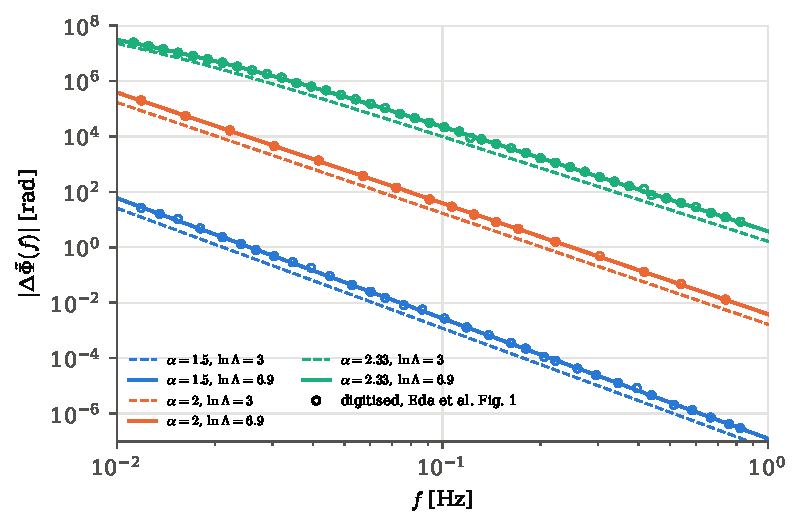
\includegraphics[width=0.8\linewidth]{figures/ch10/eda_dephasing.pdf}
\caption{The Fourier-phase difference between an inspiral in a dark-matter spike and in vacuum, accumulated between
$f$ and the ISCO, for three spike slopes. Open circles: Figure~1 of Eda et al., digitised from the published PDF.
Dashed: our calculation with the Coulomb logarithm stated in their text, $\ln\Lambda=3$; it is low by the same factor
$2.3$ on every curve. Solid: with $\ln\Lambda=\ln10^3=6.9$, which reproduces the figure.}
\label{10b:fig:eda-dephasing}
\end{figure}

\paragraph{The forecast.} Eda et al.\ compute a Fisher matrix for six parameters, $\ln\mathcal A$, $t_c$, $\Phi_c$,
$\ln\mathcal M$, $\ln\alpha$ and $\ln c_\epsilon$, where $c_\epsilon$ is the strength of the friction \cite[eqs.~(37)--(38)]{Eda2015}.
Their detector is the eLISA design of the time, with arm length $10^9$\,m and the noise of their eq.~(32a), which
\pyname{lib_gw10.py} implements as \pyname{Sn_elisa}. The band runs from the frequency five years before the ISCO,
$f_{\rm ini}(\alpha)$, to $f_I$ \cite[eq.~(40)]{Eda2015}: friction speeds up the early inspiral, so a steeper spike
starts the five years at a lower frequency. We find $f_{\rm ini}=\TenBedaFiniZeroN$\,Hz for $\alpha\to0$ (the vacuum),
$\TenBedaFiniSevenN$\,Hz for $\alpha=7/3$ and $\TenBedaFiniTwoFiveN$\,Hz for $\alpha=2.5$: a plateau and then a steep fall
above $\alpha\approx2.3$, the shape of their Figure~2 (\cref{10b:fig:eda-alpha}, left). The errors are normalised to
$S/N=10$ by scaling the matrix so that $\Gamma_{\ln\mathcal A\ln\mathcal A}=\rho^2=100$
(\cref{10b:eq:fisher-blocks}). The derivatives with respect to $\ln\alpha$ and $\ln c$ are central differences of the
complete waveform, amplitude factor $L^{-1/2}$ included, as in the paper.

The comparison at $\alpha=7/3$, $S/N=10$, with their eqs.~(41a)--(41f):
\begin{center}
\small
\begin{tabular}{@{}lcccccc@{}}
\toprule
& $\Delta\mathcal A/\mathcal A$ & $\Delta t_c$ [s] & $\Delta\Phi_c$ [rad] & $\Delta\mathcal M/\mathcal M$ & $\Delta\alpha/\alpha$ & $\Delta c/c$\\\midrule
Eda et al.\ (41) & $\TenBedaPaperA$ & $\TenBedaPaperTc$ & $\TenBedaPaperPhic$ & $\TenBedaPaperMc$ & $\TenBedaPaperAlpha$ & $\TenBedaPaperC$\\
ours, $\ln\Lambda=3$ & $\TenBedaOursA$ & $\TenBedaOursTc$ & $\TenBedaOursPhic$ & $\TenBedaOursMc$ & $\TenBedaOursAlpha$ & see text\\
ours, $\ln\Lambda=6.9$ & $\TenBedaOursAN$ & $\TenBedaOursTcN$ & $\TenBedaOursPhicN$ & $\TenBedaOursMcN$ & $\TenBedaOursAlphaN$ & see text\\
\bottomrule
\end{tabular}
\end{center}
The amplitude error is $1/\rho$ by construction. The chirp mass agrees to $4\%$, the phase to $5\%$, the arrival time
to $20\%$; these three depend on the shape of the noise curve and on where the band starts, which we rebuilt from the
paper's description, not from its code. The slope settles the Coulomb logarithm: with $\ln\Lambda=3$ we get
$\Delta\alpha/\alpha=\TenBedaOursAlpha$, almost three times the published value; with $\ln\Lambda=6.9$ we get
$\TenBedaOursAlphaN$, within $5\%$ of it. A stronger friction measures the slope better, because the signature it
leaves is larger compared with the noise, and the figure and the forecast now agree on the same strength.\footnote{The
conclusion of Eda et al.\ quotes $\pm5\times10^{-6}$ for the $1\sigma$ error on $\alpha$; eq.~(41e), which we
reproduce, corresponds to $\Delta\alpha=2.8\times10^{-6}$.}

\paragraph{Example: why the amplitude's error depends on where it is defined.} Our $\Delta c/c$ is
$\TenBedaOursCN$, twenty-seven times smaller than their $\TenBedaPaperC$. The event is a disagreement in one parameter
only, the amplitude of the friction, while the slope in the same matrix agrees. What could make the error of an
amplitude differ while everything else agrees? The amplitude is not a single number until we say at which frequency
it is the amplitude. Our $c$ is $\epsilon$ at the pivot $f_p=0.05$\,Hz, inside the band: $\epsilon(f)=c\,(f/f_p)^{-n}$,
with $n=(11-2\alpha)/3$ from \eqref{10b:eq:eps-eda}. The same law, written with the amplitude $c'$ at another pivot
$f_q$, has $c'=c\,(f_q/f_p)^{-n}$. Then
\begin{align}
  \ln c'&\eqby{1}\ln c-n\ln\frac{f_q}{f_p},\nonumber\\
  \delta\ln c'&\eqby{2}\delta\ln c+\frac23\,\alpha\ln\frac{f_q}{f_p}\;\delta\ln\alpha,\nonumber\\
  \sigma^2_{\ln c'}&\eqby{3}\sigma^2_{\ln c}+2\lambda\,\Cov(\ln c,\ln\alpha)+\lambda^2\sigma^2_{\ln\alpha},
  \qquad\lambda\equiv\frac23\,\alpha\ln\frac{f_q}{f_p}.
  \label{10b:eq:pivot}
\end{align}
\begin{explain}
  \item Take the logarithm of $c'=c\,(f_q/f_p)^{-n}$.
  \item Vary both sides; $n$ depends on $\alpha$ through $\dd n=-\tfrac23\dd\alpha=-\tfrac23\alpha\,\dd\ln\alpha$.
  \item The variance of a linear combination $\delta\ln c+\lambda\,\delta\ln\alpha$ (the propagation rule of
        \cref{10a:sec:reparam}).
\end{explain}
The error of the amplitude grows quadratically with the lever arm $\lambda$, the logarithmic distance between the two
pivots. Where is Eda et al.'s pivot? Their $c_\epsilon$ multiplies $x^{(11-2\alpha)/2}$, where $x$ is the orbital radius
in units of $R_*$, the radius at which the spike, extrapolated inwards, would enclose a mass equal to the black hole's
\cite[eqs.~(10b), (17), (18), (28d)--(28f)]{Eda2015}. For their halo $R_*=\TenBedaRstarN$\,pc. The orbit in the band has
a radius of about $10^{-8}$\,pc, so their amplitude is defined eight decades in radius, and twelve in frequency
($f_*=\TenBedaFstarN$\,Hz; Eda et al.'s pivot, not LISA's transfer frequency), away from the data. The script evaluates \eqref{10b:eq:pivot} at $f_*$:

\pyfile[firstline=179,lastline=190,firstnumber=179]{code/ch10/13_eda2015.py}{The amplitude error at another pivot}

\noindent Line 181 is $R_*$, from $4\pi\rho_{\rm sp}r_{\rm sp}^\alpha R_*^{3-\alpha}/(3-\alpha)=M_{\rm BH}$; line 182 is
Kepler's law at $R_*$; lines 183--185 are \eqref{10b:eq:pivot}. At $f_*$ the error is $\TenBedaCstarN$, against their
$\TenBedaPaperC$: the factor of twenty-seven has become ten per cent. In the other direction, the pivot at which $c$ and
$\alpha$ decorrelate, $f_q=\TenBedaFbestN$\,Hz, gives the smallest possible error, $\TenBedaCbestN$. The decorrelation
pivot sits where the signal-to-noise ratio accumulates, for the same reason that Knox's tilt and amplitude decorrelate
at $\ell_*\approx210$ in \cref{10a:sec:knox}: an amplitude measured where the data are is not dragged by the
uncertainty of the slope. At our $f_p=0.05$\,Hz the correlation between $\ln c$ and $\ln\alpha$ is already
$\TenBedaCorrACN$; at $f_*$ it is essentially one.

\begin{pitfall}[An amplitude without a pivot has no error bar]
When a power law has a free exponent, the error of its amplitude depends on the frequency (or scale) at which the
amplitude is defined, and grows with the logarithmic distance from the data. Quote amplitudes at a pivot inside the
band, ideally the decorrelation pivot, or quote the pivot with the error.
\end{pitfall}

\paragraph{Example: how shallow a spike can be measured.} Repeating the forecast for every slope gives
$\Delta\alpha/\alpha$ as a function of $\alpha$ at $S/N=10$ (\cref{10b:fig:eda-alpha}, right). The error falls by many
orders of magnitude between $\alpha=1.4$ and $2.4$, because $\epsilon\propto\rho_{\rm sp}(r_{\rm sp}/R)^\alpha$ grows rapidly with
$\alpha$ at the tiny radii of the band, and turns up near $\alpha\approx2.5$ where the band start drops and the binary
spends its five years with friction in charge. Eda et al.\ state that the slope is measured to $10\%$ down to
$\alpha\approx1.7$ \cite[Sec.~IV D]{Eda2015}. We find $\alpha=\TenBedaAlphaTenN$ (and $\TenBedaAlphaTen$ with
$\ln\Lambda=3$).

\begin{figure}[htbp]
\centering
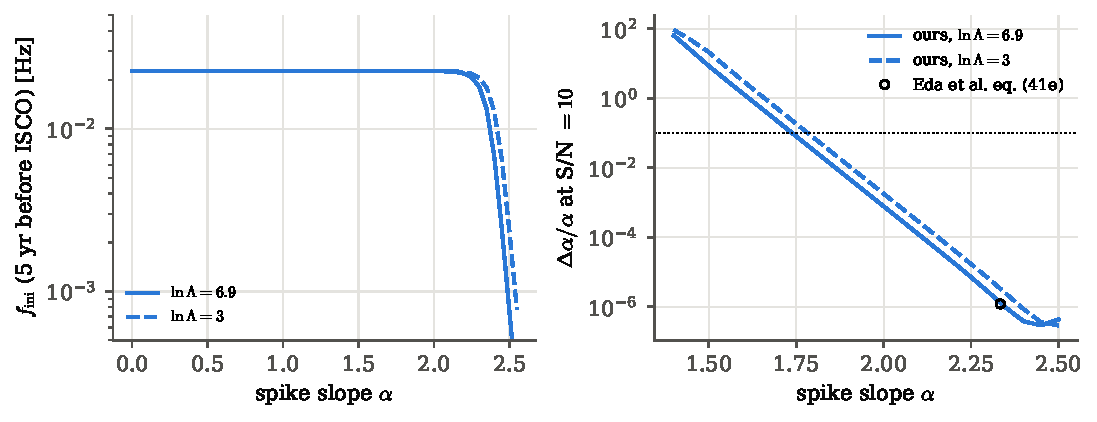
\includegraphics[width=\linewidth]{figures/ch10/eda_alpha.pdf}
\caption{Left: the frequency at which the last five years before the ISCO begin, against the spike slope; friction makes
steep spikes start lower. Right: the forecast relative error on the slope at $S/N=10$ with the eLISA noise of Eda et
al., for the two Coulomb logarithms; the circle is their eq.~(41e) and the dotted line the $10\%$ level, crossed near
$\alpha=1.7$ as they state.}
\label{10b:fig:eda-alpha}
\end{figure}

\subsection{Kim et al.\ 2023: a wave-like halo, LISA, and a posterior}
\label{10b:sec:kim}

\paragraph{The model.} The benchmark of Kim et al.\ \cite[Table~I]{Kim2023} is a $m_1=10^4M_\odot$ black hole with a
$m_2=1\,M_\odot$ companion ($\mathcal M=39.8\,M_\odot$, $q=m_2/m_1=10^{-4}$) at $D_L=203$\,Mpc, in a spike of slope
$\gamma_{\rm sp}=7/3$ with density $\rho_6=25\times10^{15}M_\odot\,{\rm pc}^{-3}$ at $r_6=10^{-6}$\,pc. The dark matter
is a wave with gravitational Bohr radius $a=10^{-11}$\,pc. Each ingredient of their model has a short physical
reason, and each is a line of \pyname{14_kim2023.py}.
\begin{itemize}[itemsep=2pt,leftmargin=1.2em]
  \item \emph{Energy balance.} $\dd E_o/\dd t=-(P_{\rm GW}+\dot E_f)$ with the vacuum orbital energy
        \cite[eq.~(36)]{Kim2023}, so $\dot f=\dot f_{\rm V}(1+\epsilon)$ with $\epsilon=\dot E_f/P_{\rm GW}$, exactly
        \cref{T2a:eq:fdot-env}.
  \item \emph{Friction.} $\dot E_f=4\pi(Gm_2)^2\rho(<v)\,C/v$, with $\rho(<v)\approx0.6\rho$ the density of the slower
        particles \cite[eq.~(39)]{Kim2023}: Chandrasekhar's formula (\cref{T2a:eq:df}) with $\xi=0.6$ and the Coulomb
        logarithm replaced by a factor $C$. For particles,
        $C_p=\frac{1+\Lambda}{\Lambda}\ln\big[1+\Lambda+\sqrt{\Lambda(2+\Lambda)}\big]-\sqrt{1+2/\Lambda}$ with
        $\Lambda=v^2r/(Gm_2)$, which tends to $\ln2\Lambda-1$ for $\Lambda\gg1$ \cite[eq.~(41)]{Kim2023}. For a wave,
        $C_w(kr)=\mathrm{Cin}(2kr)-1+\sin(2kr)/2kr$ \cite[eq.~(42)]{Kim2023}, whose limits \cref{T2a:sec:forces}
        derives: friction is suppressed as $(kr)^2/3$ when the de Broglie wavelength exceeds the orbit.
  \item \emph{The density.} For particles the spike is cut off at twice the Schwarzschild radius,
        $\rho_6(r_6/r)^\gamma(1-2R_S/r)^\gamma$. For a wave, the modes of low angular momentum fall into the hole: a mode
        $(n,\ell)$ decays at a rate $\Gamma_{n\ell}$ that grows steeply as $\ell$ falls \cite[eq.~(31)]{Kim2023}, and the
        modes with $2\Gamma_{n\ell}t_{\rm halo}>1$ are gone after the halo's age. The lowest surviving angular momentum
        $\ell_c$ sets an inner radius $R_c=a\,\ell_c(\ell_c+1)$ and the profile $\rho_6(r_6/r)^\gamma(1-R_c/2r)^\gamma$
        \cite[eq.~(40)]{Kim2023}. We solve $2\max_n\Gamma_{n\ell}t_{\rm halo}=1$ for continuous $\ell$ with
        $t_{\rm halo}=13.6$\,Gyr (a halo formed at $z\approx20$) and find $\ell_c=\TenBkimEllW$,
        $\TenBkimEllX$ and $\TenBkimEllY$ for $a=10^{-11}$, $10^{-10}$ and $10^{-9}$\,pc, that is particle masses
        $mc^2=\TenBkimMassW$, $\TenBkimMassX$ and $\TenBkimMassY$\,eV (their figure labels: $9\times10^{-14}$,
        $3\times10^{-14}$, $9\times10^{-15}$\,eV).
  \item \emph{Backreaction.} The friction cannot dissipate more energy than the halo can absorb. Kim et al.\ cap it by
        the rate at which the companion sweeps through the binding energy of the shells it crosses:
        $\dot E_f\to(1/\dot E_f+2/\dot U)^{-1}$, a smooth minimum of the two \cite[eq.~(43)]{Kim2023}.
\end{itemize}
The cap needs one more step, because $\dot U$ depends on how fast the orbit shrinks, which depends on the capped
friction itself. Write $x$ for the capped friction power. A shell of thickness $\Delta r$ at $r$ has binding energy
$\Delta U=G[m_1+m_{\rm enc}(r)]\,4\pi r^2\rho\,\Delta r/r$, and the orbit crosses shells at the rate $|\dot r|$:
\begin{align}
  \dot U&\eqby{1}\frac{G(m_1+m_{\rm enc})\,4\pi r^2\rho}{r}\,|\dot r|
  \eqby{2}\frac{G(m_1+m_{\rm enc})\,4\pi r\rho\cdot2r^2}{Gm_1m_2}\,(P_{\rm GW}+x)\equiv\kappa\,(P_{\rm GW}+x),\nonumber\\
  \frac1x&\eqby{3}\frac1{\dot E_f}+\frac{2}{\kappa(P_{\rm GW}+x)}
  \quad\Longrightarrow\quad
  \kappa x^2-\big[\kappa(\dot E_f-P_{\rm GW})-2\dot E_f\big]x-\kappa\dot E_fP_{\rm GW}\eqby{4}0 .
  \label{10b:eq:backreaction}
\end{align}
\begin{explain}
  \item The binding energy per unit radius times the radial speed.
  \item $E_o=-Gm_1m_2/2r$ gives $|\dot r|=|\dot E_o|/(\dd E_o/\dd r)=(P_{\rm GW}+x)\,2r^2/(Gm_1m_2)$; $G$ cancels.
  \item Kim et al.'s eq.~(43) with $\dot U$ from step (2).
  \item Multiply by $x\,\dot E_f\,\kappa(P_{\rm GW}+x)$ and collect powers of $x$; the positive root is the capped friction.
\end{explain}
Kim et al.\ do not say how they evaluate $\dot U$; taking the radial speed from the total power, as here, is the
self-consistent choice, and the quadratic \eqref{10b:eq:backreaction} is lines 108--110 of the script.

\paragraph{Example: the dephasing curves.} \Cref{10b:fig:kim-dephasing} compares $|\Delta\Phi|$ of
\eqref{10b:eq:kim49} with Figure~3 (top) of Kim et al., digitised by colour. For the particle halo the median of
$\log_{10}(\text{ours}/\text{theirs})$ is $\TenBkimDevMedP$ and the largest deviation $\TenBkimDevMaxP$\,dex; for the
wave halo with $a=10^{-11}$\,pc, $\TenBkimDevMedW$ and $\TenBkimDevMaxW$; for $a=10^{-10}$\,pc, $\TenBkimDevMedX$ and
$\TenBkimDevMaxX$. For $a=10^{-9}$\,pc the median deviation is $\TenBkimDevMedY$\,dex: there the inner cut-off $R_c$
lies inside the band, the curve plunges where the companion reaches $R_c/2$, and a small change in $\ell_c$ moves the
plunge enough to change the phase there by large factors; in \cref{10b:fig:kim-dephasing} our green curve plunges slightly earlier than theirs. The comparison is therefore a test of the decay rates as
much as of the friction. At $10$\,mHz the particle halo has dephased the signal by $\TenBkimDphiCentP$\,rad and the wave
halo with $a=10^{-11}$\,pc by $\TenBkimDphiCentW$\,rad. Everything in the figure depends on $\epsilon$ only through
\eqref{10b:eq:kim49}, so this agreement confirms the whole chain from the decay rates to the backreaction cap.

\begin{figure}[htbp]
\centering
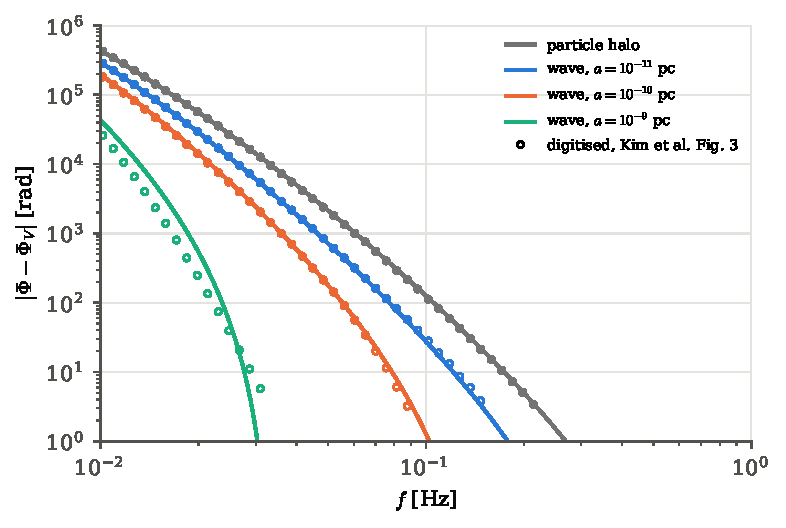
\includegraphics[width=0.8\linewidth]{figures/ch10/kim_dephasing.pdf}
\caption{The time-domain phase lost between $f$ and the ISCO by the $10^4+1\,M_\odot$ inspiral in a particle halo (grey)
and in wave halos of three Bohr radii, against the published Figure~3 of Kim et al.\ (open circles, digitised). The
larger the Bohr radius, the more inner modes the black hole has swallowed and the earlier the friction switches off.}
\label{10b:fig:kim-dephasing}
\end{figure}

\paragraph{Example: the signal-to-noise ratio.} With the sky-averaged amplitude $\sqrt{4/5}\,A(f)$
\cite[eqs.~(44)--(45)]{Kim2023} (the $4/5$ is the average over the orbit's inclination, \eqref{T2g:eq:four-fifths};
the sky and polarisation average sits in the noise curve, \cref{T2g:sec:detector}), the Robson et al.\ noise with four-year Galactic confusion (\cref{10b:sec:robson,T2a:sec:lisa}), and the band
from five years before the ISCO, $f_{5\rm yr}=\TenBkimfFive$\,Hz, to $\min(1\,{\rm Hz},f_I)=\TenBkimfUp$\,Hz, we find
$\rho=\TenBkimSNR$. They state $\rho\simeq15$.

\paragraph{Example: the forecast against their posterior.} Kim et al.\ do not compute a Fisher matrix. They inject the
benchmark signal without noise, $d=h(\params_{\rm true})$ (the ``median experiment'' of \cref{10b:sec:validity}), and
sample the posterior of $(\mathcal M,\log_{10}q,\rho_6,\gamma_{\rm sp},\log_{10}a)$ with a nested sampler, maximising the
likelihood over the arrival time and the phase and fixing the distance at its best value \cite[eqs.~(50)--(53),
Fig.~4]{Kim2023}. Their Figure~4 quotes the $2.5\%$ and $97.5\%$ quantiles of each marginal. We turn each $95\%$
interval into a Gaussian-equivalent width by dividing it by $3.92$, and compare with the Fisher matrix of eight
parameters, the five plus $(\ln\mathcal A,t_c,\phi_c)$, with the derivatives taken by central differences of the
complete waveform (amplitude factor $(1+\epsilon)^{-1/2}$ included):

\pyfile[firstline=212,lastline=221,firstnumber=212]{code/ch10/14_kim2023.py}{The waveform whose derivatives make the Fisher matrix}

\noindent Line 217 is the integrand of \eqref{10b:eq:kim49} divided by $f'$, and line 219 builds the dark-matter part of
$\tilde\Phi$ from it as in \eqref{10b:eq:phitilde}; line 221 returns $\ln\tilde h$ up to a constant, whose real part is the
slower-sweep amplitude and whose imaginary part is the phase. Halving and doubling the steps changes no error by
more than $\TenBkimStepDev$. At the Gaussian level, maximising over $(t_c,\phi_c,\ln\mathcal A)$ and marginalising over
them give the same widths (both are the Schur complement of \cref{10a:sec:marginal}), so the comparison is fair. The
result (\cref{10b:fig:kim-fisher}):
\begin{center}
\small
\begin{tabular}{@{}lccccc@{}}
\toprule
& $\mathcal M$ [$M_\odot$] & $\log_{10}q$ & $\rho_6$ [$10^{15}M_\odot{\rm pc}^{-3}$] & $\gamma_{\rm sp}$ & $\log_{10}a$\\\midrule
posterior (Kim et al.) & $\TenBkimPostMc$ & $\TenBkimPostLq$ & $\TenBkimPostRho$ & $\TenBkimPostGam$ & $\TenBkimPostLa$\\
Fisher (ours) & $\TenBkimFishMc$ & $\TenBkimFishLq$ & $\TenBkimFishRho$ & $\TenBkimFishGam$ & $\TenBkimFishLa$\\
ratio & $\TenBkimRatioMc$ & $\TenBkimRatioLq$ & $\TenBkimRatioRho$ & $\TenBkimRatioGam$ & $\TenBkimRatioLa$\\
\bottomrule
\end{tabular}
\end{center}
The order of magnitude is right for every parameter, and the Fisher matrix finds the same structure as the posterior:
a correlation of $\TenBkimCorrRhoGam$ between $\rho_6$ and $\gamma_{\rm sp}$ and of $\TenBkimCorrRhoLq$ between $\rho_6$
and $\log_{10}q$, the two degeneracies Kim et al.\ point out in their Figure~4. But every Fisher width is smaller,
by a factor $1.4$ to $5.5$. The matrix is nearly singular (the ratio of its largest to smallest eigenvalue, after
scaling to unit diagonal, is $\TenBkimCond$), and along its long axis a $1\sigma$ step moves $\rho_6$ by a quarter of its
value and $\gamma_{\rm sp}$ by $0.09$, far beyond the region where the waveform is linear in the parameters.
\Cref{10b:sec:validity} quantifies this and shows that it, not the code, is the cause. For a particle halo of the same
density the four common errors would be $\TenBkimPartMc\,M_\odot$, $\TenBkimPartLq$, $\TenBkimPartRho$ and
$\TenBkimPartGam$: the dense inner spike that the wave halo has lost carries most of the information.

\begin{figure}[htbp]
\centering
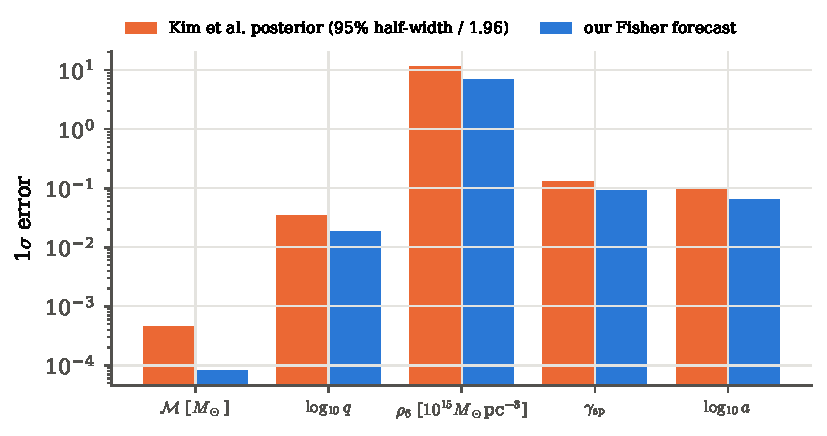
\includegraphics[width=0.78\linewidth]{figures/ch10/kim_fisher.pdf}
\caption{The $1\sigma$ widths of the five halo and binary parameters for the benchmark of Kim et al.\ ($\rho\approx15$):
their nested-sampling posterior (Figure~4, $95\%$ half-width divided by $1.96$) and our Fisher forecast. The forecast is
right to within a factor of a few and too optimistic everywhere, most for the chirp mass, whose posterior is skewed by
its correlation with the mass ratio and the density.}
\label{10b:fig:kim-fisher}
\end{figure}

\subsection{Paper against ours}
\label{10b:sec:paper-vs-ours}

\Cref{10b:tab:paper-vs-ours} collects every published gravitational-wave number we have reproduced. Where we
agree to better than the precision of reading a plotted line, the paper's model has been rebuilt correctly. Where we
disagree, the disagreement has been traced to a cause: a fitted response function (Robson et al.\ above the transfer frequency $f_*$, \cref{T2g:eq:transfer}), a
rounded amplitude (the printed $h_{\rm GB}$), an abbreviated Coulomb logarithm and a pivot far outside the band (Eda et
al.), or the breakdown of the Gaussian approximation (Kim et al.).

\begin{table}[htbp]
\centering
\small
\renewcommand{\arraystretch}{1.15}
\begin{tabular}{@{}>{\raggedright\arraybackslash}p{0.15\linewidth}>{\raggedright\arraybackslash}p{0.37\linewidth}>{\raggedright\arraybackslash}p{0.16\linewidth}>{\raggedright\arraybackslash}p{0.24\linewidth}@{}}
\toprule
paper & quantity & published & ours\\\midrule
Robson et al.\ 2019 & $\sqrt{S_n}$, $1$--$30$\,mHz (Fig.~4) & curve & within $\TenBrobDevLow\%$\\
& J0651 signal-to-noise ratio & $140$ & $\TenBrobJsnr$\\
& GW150914-like band, 5\,yr before merger & $16$--$29$\,mHz & $\TenBrobGWfFive$--$\TenBrobGWfOne$\,mHz\\
& $10^6M_\odot$ pair at $z=3$, 1\,yr before & $2.93\times10^{-5}$\,Hz & $\TenBrobBigf$\,Hz\\
Cutler \& Flanagan 1994 & Table I, 25 errors at $\rho=10$ & table & all within $\TenBcfMaxDev\%$\\
Eda et al.\ 2015 & $\Delta\tilde\Phi(f)$, three slopes (Fig.~1) & curves & $\TenBedaDevMedCN$ to $\TenBedaDevMedAN$\,dex ($\ln\Lambda=6.9$)\\
& $\Delta\mathcal M/\mathcal M$ at $S/N=10$ & $3.1\times10^{-7}$ & $\TenBedaOursMcN$\\
& $\Delta\alpha/\alpha$ at $S/N=10$ & $1.2\times10^{-6}$ & $\TenBedaOursAlphaN$\\
& $\Delta c_\epsilon/c_\epsilon$ (their pivot) & $5.9\times10^{-5}$ & $\TenBedaCstarN$\\
& $\Delta t_c$, $\Delta\Phi_c$ & $1.0$\,s, $1.3$ & $\TenBedaOursTcN$\,s, $\TenBedaOursPhicN$\\
& slope measured to $10\%$ & $\alpha\approx1.7$ & $\TenBedaAlphaTenN$\\
Kim et al.\ 2023 & $|\Delta\Phi(f)|$, particle and $a=10^{-11}$\,pc (Fig.~3) & curves & $\TenBkimDevMedP$, $\TenBkimDevMedW$\,dex\\
& signal-to-noise ratio & $\simeq15$ & $\TenBkimSNR$\\
& widths of $(\mathcal M,\log q,\rho_6,\gamma,\log a)$ & Fig.~4 & Fisher $\times(\TenBkimRatioMc$--$\TenBkimRatioGam)$\\
\bottomrule
\end{tabular}
\caption{Published numbers against our reproductions. Deviations in dex are medians of $\log_{10}(\text{ours}/\text{theirs})$
along the digitised curves.}
\label{10b:tab:paper-vs-ours}
\end{table}
\section{When the Fisher ellipse lies}
\label{10b:sec:validity}

The benchmark of Kim et al.\ ended on an uncomfortable note (\cref{10b:sec:kim}): the Fisher matrix found the right
parameters to worry about and the right correlations, but every width came out too small, by factors up to five
compared with the posterior that a sampler drew from the same model. A forecast that is optimistic by a factor of
five can turn ``LISA will measure the dark-matter density'' into ``LISA will see that there is something there''. So
before any detectability map is believed, the question in words is:
\begin{center}
\emph{for this source, at this signal-to-noise ratio, does the Fisher ellipse describe the posterior we would actually
obtain, and if not, where does it fail?}
\end{center}
Of Vallisneri's three readings of $\Gamma^{-1}$ (\cref{10a:sec:cr-reach}) \cite{Vallisneri2008}, the one a forecast
relies on is the third: the covariance of the posterior from one experiment. The posterior is something we can compute
exactly, by sampling, so the question has an answer that does not depend on approximations.

\subsection{The linearised signal}
\label{10b:sec:lsa}

\paragraph{The median experiment.} To compare a forecast with a posterior we need data. Papers, Kim et al.\ and
Coogan et al.\ among them \cite{Kim2023,Coogan2022}, use the data with the noise set to zero, $d=h(\params_0)$, and we
do the same. This is not a claim that there is no noise. A noise realisation moves the peak of the posterior away
from $\params_0$, by a random amount whose covariance (at high signal-to-noise ratio) is $\Gamma^{-1}$ itself, but it
leaves the shape of the posterior almost unchanged. Setting $n=0$ removes the random shift and keeps the shape, the
quantity a forecast is about. The noise-free data stand for the typical, or median, experiment.

\paragraph{When is the likelihood exactly the Fisher Gaussian?} With $d=h_0\equiv h(\params_0)$ the likelihood
\eqref{10b:eq:gw-like} is $\ln\Like(\params)=-\tfrac12(\Delta h|\Delta h)$, with $\Delta h\equiv h(\params)-h_0$. Expand the
signal around the truth, $\Delta h=\Delta\theta^i\partial_ih+R$, where the first term is the tangent (linear) part, the sum
over $i$ is implied, and $R$ is everything of second order and higher. Then
\begin{align}
  -2\ln\Like(\params)
  &\eqby{1}\big(\Delta\theta^i\partial_ih+R\,\big|\,\Delta\theta^j\partial_jh+R\big)\nonumber\\
  &\eqby{2}\Delta\theta^i\Delta\theta^j\,(\partial_ih|\partial_jh)+2\,\Delta\theta^i(\partial_ih|R)+(R|R)\nonumber\\
  &\eqby{3}\Delta\params\T\Gamma\,\Delta\params+2\,\Delta\theta^i(\partial_ih|R)+(R|R).
  \label{10b:eq:lsa}
\end{align}
\begin{explain}
  \item Insert the expansion of $\Delta h$ into $-2\ln\Like=(\Delta h|\Delta h)$.
  \item The inner product is bilinear and symmetric.
  \item $(\partial_ih|\partial_jh)=\Gamma_{ij}$, \eqref{10b:eq:gw-fisher}.
\end{explain}
If the signal were exactly linear in the parameters, $R=0$, the log-likelihood would be exactly the quadratic
$-\tfrac12\Delta\params\T\Gamma\Delta\params$, and with a flat prior the posterior would be exactly the Gaussian of covariance
$\Gamma^{-1}$, at any signal-to-noise ratio. This is the \newterm{linearised-signal approximation} (LSA): it is the whole
content of a Fisher forecast. Everything that makes the forecast wrong is in $R$.

Geometrically (\cref{10b:fig:manifold}), as $\params$ varies the waveforms $h(\params)$ trace out a curved surface in the
space of all possible data, and the noise is a cloud of radius about one around the true signal, in the units of the
inner product (\cref{10b:eq:noise-overlap}). The Fisher matrix replaces the surface by its tangent plane. That is
harmless if the surface is flat across the cloud and fatal if it bends within it.

\begin{figure}[htbp]
\centering
\begin{tikzpicture}[scale=1.05]
  \begin{scope}
    \fill[softgray!15] (0,0) circle (1.25);
    \draw[softgray] (0,0) circle (1.25);
    \draw[form,thick] ([shift={(-2,0)}]-62:2) arc (-62:62:2);
    \draw[bdry,dashed] (0,-1.9) -- (0,1.9);
    \fill (0,0) circle (1.6pt);
    \node[lbl,anchor=east] at (-0.08,-0.22) {$h_0$};
    \node[lbl,formblue,anchor=east] at (-1.05,1.65) {signals $h(\params)$};
    \node[lbl,bdryred,anchor=west] at (0.08,1.75) {tangent plane (Fisher)};
    \node[lbl,anchor=north] at (0,-2.1) {low $\rho$: the surface bends inside the cloud};
  \end{scope}
  \begin{scope}[xshift=6.2cm]
    \fill[softgray!15] (0,0) circle (0.36);
    \draw[softgray] (0,0) circle (0.36);
    \draw[form,thick] ([shift={(-2,0)}]-62:2) arc (-62:62:2);
    \draw[bdry,dashed] (0,-1.9) -- (0,1.9);
    \fill (0,0) circle (1.6pt);
    \node[lbl,anchor=east] at (-0.42,-0.3) {$h_0$};
    \node[lbl,anchor=north] at (0,-2.1) {high $\rho$: flat across the cloud};
  \end{scope}
\end{tikzpicture}
\caption{The linearised-signal approximation in the space of data. The blue arc is the family of signals $h(\params)$ as
one parameter varies, the dashed red line its tangent at the true signal $h_0$, and the grey disc the region of radius
one that the noise fills. When the signal is weak compared with the noise, the true family departs from its tangent
inside the disc and the Fisher Gaussian is wrong; when it is strong, the disc is small and the tangent is all that
matters.}
\label{10b:fig:manifold}
\end{figure}

\paragraph{A test of the approximation.} How large may $R$ be? The Fisher $1\sigma$ ellipsoid is the surface
$\Delta\params\T\Gamma\Delta\params=1$, where the forecast says the log-likelihood has fallen by $\tfrac12$. Vallisneri
proposes to walk over that surface and compute there the noise-weighted size of the nonlinear part,
\begin{equation}
  \lvert\log r\rvert=\tfrac12\,(R\,|\,R),\qquad R=h(\params)-h_0-\Delta\theta^i\partial_ih,
  \label{10b:eq:logr}
\end{equation}
and to accept the forecast if $\lvert\log r\rvert\lesssim0.1$ everywhere on it \cite[eq.~(47)]{Vallisneri2008}. He shows that
this is the logarithm of the ratio of the exact and the linearised likelihood, averaged over the noise realisations
that would put the best fit on that surface. In words: on the boundary that the forecast calls ``one sigma'', the
true signals must differ from their tangent-plane stand-ins by much less than the noise. Since the $1\sigma$ surface
shrinks as $1/\rho$ and $R$ is quadratic in $\Delta\params$, $R$ shrinks as $\rho\cdot\rho^{-2}$ and $\lvert\log r\rvert$ falls as
$1/\rho^2$: every forecast becomes right at high enough signal-to-noise ratio, and the test says how high is high
enough.

\begin{keyidea}[When to trust a Fisher forecast]
A Fisher forecast is the posterior of the linearised signal. Check it on its own $1\sigma$ surface: the part of the
signal change that is not linear in the parameters must have noise-weighted size $\tfrac12(R|R)\lesssim0.1$ there.
Where it fails, sample the posterior.
\end{keyidea}

\paragraph{Example: the benchmark of Kim et al.} The script \pyname{14_kim2023.py} draws $300$ random points on the
$1\sigma$ surface of its eight-parameter Fisher matrix and evaluates \eqref{10b:eq:logr} with the complete waveform. The
median is $\lvert\log r\rvert=\TenBkimLogrMed$ (the largest $\TenBkimLogrMax$), and every point fails the test: not by a
little, but by three orders of magnitude. The reason is the near-degeneracy of $\rho_6$ and $\gamma_{\rm sp}$ (their
Fisher correlation is $\TenBkimCorrRhoGam$): along it the $1\sigma$ surface stretches to changes of the density by a
quarter and of the slope by a tenth, and there the dephasing, a strongly nonlinear function of both, is nothing like
its tangent. Repeating the test with the surface scaled down, as it would be for a louder source, the median falls to
$\TenBkimLogrHundred$ at a hundred times the signal-to-noise ratio and reaches $0.1$ only near $\rho\approx\TenBkimSNRneeded$.
For this benchmark the honest forecast is the posterior; the Fisher matrix is a guide to which parameters are
degenerate, not to how large the errors are.

\subsection{A chain against the ellipse}
\label{10b:sec:fisher-vs-mh}

The criterion says whether to trust the forecast; it does not say how wrong it is. For that we sample the posterior
with the Metropolis--Hastings chain of \cref{ch:09} and compare. To keep the chain small, the problem is reduced to
the four parameters that matter for an environment.

\paragraph{The set-up.} The source is the $10^3+1.4\,M_\odot$ binary of \cref{10b:sec:benchmark}, observed by LISA over
its last five years from $f_{\rm lo}=\TenBmhflo$\,mHz. Its phase is the 1.5PN phase \eqref{10b:eq:psi-pn} (the vacuum template through 1.5 post-Newtonian order,
\cref{T2g:sec:pn}, with chirp mass $\mathcal M$ and the coalescence time and phase $t_c$, $\phi_c$ of
\cref{T2g:sec:tc-phic}) plus a power-law environment (the ppE term of \cref{T2g:eq:ppe-rule}) written through its
size at the start of the band,
\begin{equation}
  \Psi(f)=\Psi_{\rm 1.5PN}(f;\mathcal M,\eta,t_c,\phi_c)+A\,\Big(\frac{u}{u_{\rm lo}}\Big)^{b},
  \qquad A=\delta\Psi(f_{\rm lo}),
  \label{10b:eq:mh-model}
\end{equation}
with $u=\pi G\mathcal Mf/c^3$ as in \cref{10b:sec:env} and $u_{\rm lo}$ its value at $f_{\rm lo}$. Writing the amplitude
as the phase shift at $f_{\rm lo}$, rather than as $\beta$, keeps it of order radians for every $b$. The free parameters
are $(\ln\mathcal M,t_c,A,b)$; $\eta$ is held at its true value, the amplitude $\ln\mathcal A$ decouples
(\cref{10b:sec:fisher-structure}) and is held too, and $\phi_c$ is integrated out analytically. The truth is a
friction-like effect with $b=-4$ and $A=-\TenBmhAtrue$\,rad, three times the Fisher error $\sigma_A=\TenBmhSigATen$\,rad
at $\rho=10$. Then the source is moved closer, $\rho=10$, $20$, $40$, $80$, with the same $A$.

\paragraph{Integrating out the phase.} The phase $\phi_c$ is a nuisance with a flat prior on $[0,2\pi)$, and it can be
removed exactly. The question in words: what is the probability of the data regardless of $\phi_c$? With
$\tilde h(\params,\phi_c)=\tilde h(\params)e^{i\phi_c}$ (the phase enters $\Psi$ as $-\phi_c$), noise-free data $d=h_0$,
equal amplitudes $(h|h)=(h_0|h_0)=\rho^2$, and the weight $w$ of \eqref{10b:eq:fisher-blocks},
\begin{align}
  (d-h\,|\,d-h)&\eqby{1}(h_0|h_0)+(h|h)-2(h_0|h)
  \eqby{2}2\rho^2-2\rho^2\,\mathrm{Re}\big[Z\,e^{-i\phi_c}\big],\nonumber\\
  Z(\params)&\equiv\int w(f)\,e^{i[\Psi(f;\params)-\Psi_0(f)]}\,\dd f,\nonumber\\
  \Like(\params)&\eqby{3}\frac1{2\pi}\int_0^{2\pi}e^{-\rho^2+\rho^2|Z|\cos(\phi_c-\arg Z)}\,\dd\phi_c
  \eqby{4}e^{-\rho^2}\,I_0\big(\rho^2|Z(\params)|\big).
  \label{10b:eq:phase-marg}
\end{align}
\begin{explain}
  \item Expand the inner product; it is symmetric.
  \item $(h_0|h)=4\,\mathrm{Re}\int\tilde h_0\tilde h^*/S_n\,\dd f$ with $\tilde h_0\tilde h^*=|\tilde h|^2e^{i(\Psi-\Psi_0)}e^{-i\phi_c}$, and
        $4|\tilde h|^2/S_n=\rho^2w$.
  \item Marginalise $e^{-(d-h|d-h)/2}$ over $\phi_c$ with the flat prior $1/2\pi$; write $Z=|Z|e^{i\arg Z}$.
  \item $\frac1{2\pi}\int_0^{2\pi}e^{x\cos\varphi}\dd\varphi=I_0(x)$, the modified Bessel function; the shift by $\arg Z$ does not
        change an integral over a full period.
\end{explain}
$\lvert Z\rvert\le1$ is the overlap of the trial phase with the true one, averaged with the signal-to-noise weight: it is
one when the phases agree up to a constant and falls as they drift apart. For large argument
$\ln I_0(x)\approx x-\tfrac12\ln2\pi x$, so $\ln\Like\approx-\rho^2(1-|Z|)$: the likelihood penalises the lost overlap times
$\rho^2$, the same structure as the phase-maximised likelihood of Kim et al.\ \cite[eq.~(53)]{Kim2023}. The script
\pyname{15_fisher_vs_mh.py} implements it in three lines:

\pyfile[firstline=53,lastline=60,firstnumber=53]{code/ch10/15_fisher_vs_mh.py}{The likelihood with the phase integrated out}

\noindent Line 54 is the integrand of $Z$ on the logarithmic grid (\texttt{fw} is $f\,w(f)$), line 55 the trapezoid sum,
and line 60 is $\ln\Like=\ln I_0(x)-\rho^2$, computed as $\ln(e^{-x}I_0(x))+x$ because $I_0(x)$ itself overflows for
$x=\rho^2\sim6400$. The Fisher matrix to compare with is the $5\times5$ matrix of
$(\ln\mathcal M,t_c,A,b,\phi_c)$ with $\phi_c$ removed by its Schur complement, the Gaussian version of the same
marginalisation. The chain is the sampler of \cref{ch:09}, with a proposal covariance tuned in three short runs and
then $40\,000$ steps per signal-to-noise ratio; acceptance rates are $\TenBmhAccTen$ to $\TenBmhAccEighty$, and the whole
script runs in $\TenBmhRuntime$\,s.

\paragraph{Example: the banana at $\rho=10$.} \Cref{10b:fig:mh-banana} shows the chain against the Fisher ellipses.
At $\rho=10$ the posterior is curved: larger amplitudes $|A|$ pair with flatter exponents $b$, because a flatter power law
must be larger at $f_{\rm lo}$ to produce the same phase drift where the signal-to-noise ratio accumulates. The tail
reaches $A\approx-60$\,rad and $b\approx-2.5$, far outside the $95\%$ ellipse, and on the other side it runs into the
region of steep exponents where the effect is confined to the first few millihertz. Only $\TenBmhInTen\%$ of the samples
fall inside the Fisher $68.3\%$ ellipse in the $(A,b)$ plane. The marginal standard deviations from the chain exceed
the Fisher errors by factors of $\TenBmhRATen$ for $A$, $\TenBmhRBTen$ for $b$, $\TenBmhRMcTen$ for $\ln\mathcal M$ and
$\TenBmhRTcTen$ for $t_c$. The chirp mass and the arrival time are dragged along the banana, because each point on it is
a different combination of environment and vacuum parameters that fits the same data.

\begin{figure}[htbp]
\centering
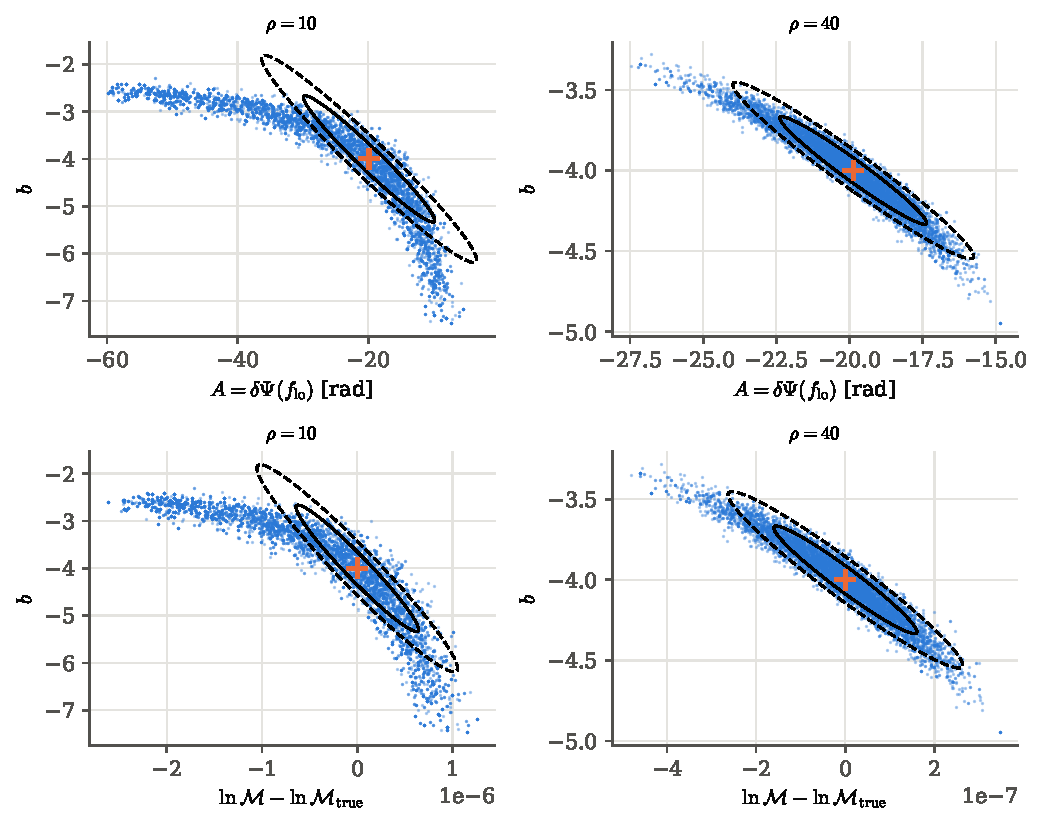
\includegraphics[width=0.9\linewidth]{figures/ch10/mh_banana.pdf}
\caption{Posterior samples from the Metropolis--Hastings chain (dots) against the Fisher $68.3\%$ and $95.4\%$ ellipses
(solid, dashed) for a power-law environment with exponent $b$ and phase shift $A$ at the start of the band. Left: at
$\rho=10$ the posterior is a curved banana that the ellipse cannot follow. Right: at $\rho=40$ it has become an
ellipse. Top: environment amplitude against exponent; bottom: chirp mass against exponent. The cross marks the truth.}
\label{10b:fig:mh-banana}
\end{figure}

\paragraph{Example: the approach to the Fisher limit.} As $\rho$ grows (\cref{10b:fig:mh-widths}), the ratio of chain to
Fisher widths falls towards one: for $A$ it is $\TenBmhRATen$, $\TenBmhRATwenty$, $\TenBmhRAForty$, $\TenBmhRAEighty$ at
$\rho=10$, $20$, $40$, $80$, and for $t_c$, the worst, $\TenBmhRTcTen$, $\TenBmhRTcTwenty$, $\TenBmhRTcForty$,
$\TenBmhRTcEighty$. The fraction of samples inside the $68.3\%$ ellipse climbs to $\TenBmhInTwenty$, $\TenBmhInForty$ and
$\TenBmhInEighty\%$. The analogue of Vallisneri's test for this experiment, the difference between the actual fall of
$\ln\Like$ on the Fisher $1\sigma$ surface and the $\tfrac12$ the forecast predicts (median over $200$ points), is
$\TenBmhLogrTen$, $\TenBmhLogrTwenty$, $\TenBmhLogrForty$ and $\TenBmhLogrEighty$: it crosses $0.1$ between $\rho=10$ and
$20$. Here it falls roughly as $1/\rho$, not $1/\rho^2$, because the noise-free drop contains the cross term
$\Delta\theta^i(\partial_ih|R)$ of \eqref{10b:eq:lsa}, which is first order in $R$.

Notice what the numbers say together. At $\rho=20$ the median test is already passed, yet the marginal widths are
still $20$ to $100\%$ larger than the forecast. The median over the $1\sigma$ surface hides the directions where the
surface bends most, and the marginal widths are set by the tails. This is why Vallisneri asks for the criterion to
hold \emph{everywhere} on the surface, not on average, and why he calls it a consistency check rather than a guarantee
\cite[Sec.~VI]{Vallisneri2008}. For environmental effects at the signal-to-noise ratios LISA expects for these sources,
a signal-to-noise ratio of ten to a few tens, the Fisher error is optimistic by factors of up to two to four, and most so for the vacuum
parameters it is correlated with.

\begin{figure}[htbp]
\centering
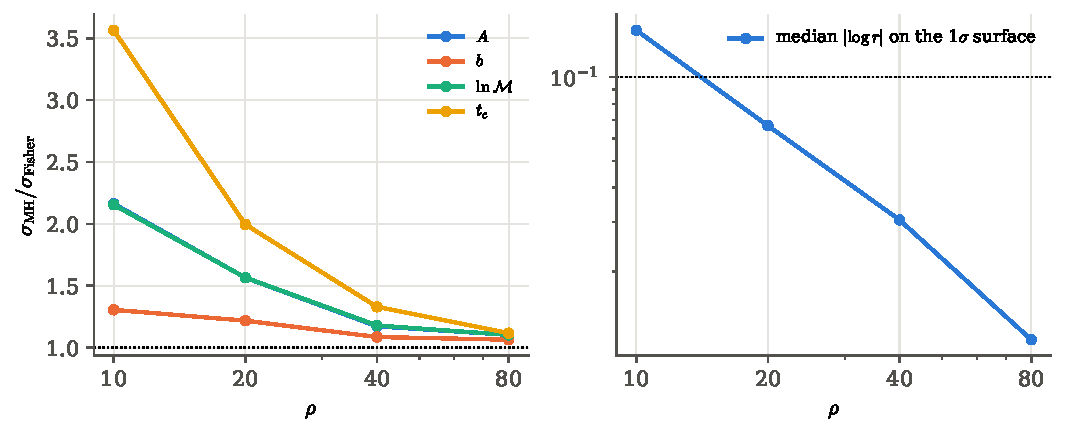
\includegraphics[width=0.9\linewidth]{figures/ch10/mh_widths.pdf}
\caption{Left: marginal standard deviation from the chain divided by the Fisher error, for the four parameters, as the
same source is moved closer. All ratios fall towards one, slowest for the arrival time. Right: the median
mismatch between the exact and the Fisher log-likelihood on the Fisher $1\sigma$ surface; the dotted line is
Vallisneri's threshold of $0.1$.}
\label{10b:fig:mh-widths}
\end{figure}

\paragraph{Example: a one-sided effect on a vacuum signal.} Friction, accretion and migration all take energy from
the orbit; none gives it back. Their phase shift therefore has a known sign ($A\le0$ in our convention), and the
right prior is one-sided. Suppose the source is in vacuum, $A=0$, at the benchmark distance ($\rho=\TenBppSNR$), with
$b=-4$ known. The Fisher matrix says $\sigma_A=\TenBmhVacSig$\,rad, a symmetric Gaussian centred on zero. The posterior
cannot be: half of that Gaussian lies at $A>0$, which the prior forbids. A chain with the prior $A\le0$ finds a
one-sided posterior piled against the boundary, with mean $|A|=\TenBmhVacMean$\,rad and a $95\%$ upper limit
$|A|<\TenBmhVacUpper$\,rad, that is $\TenBmhVacUpperRatio\,\sigma_A$. A half-Gaussian of the Fisher width would give $1.96\,\sigma_A$;
most of the excess is the nonlinearity of the previous example at $\rho\approx13$. The forecast question for a non-detection is
``what upper limit would we set?'', and the Fisher error answers it only after the prior boundary and the
nonlinearity have been put in by hand.

\begin{pitfall}[A Fisher ellipse knows nothing about boundaries]
The Fisher matrix is computed from derivatives at one point and assumes every direction is open. A parameter with a
physical boundary (a density that cannot be negative, a dissipative effect of fixed sign, a slope confined to a
range by the formation history) has a posterior that the ellipse cannot represent near the boundary, and the
published posteriors of Kim et al.\ show such skewed marginals, with long one-sided tails, for $\rho_6$ and $\log_{10}a$.
\end{pitfall}

\paragraph{Where the Fisher forecast fails, in one list.} The examples above and those of \cref{10b:sec:kim} show
four distinct mechanisms. Low signal-to-noise ratio makes the signal surface bend within the noise (the banana).
Near-degenerate parameters stretch the $1\sigma$ ellipsoid into the nonlinear region even at moderate $\rho$ (Kim's
$\rho_6$--$\gamma_{\rm sp}$). Prior boundaries cut the posterior (one-sided effects). And separate parameter regions that
fit equally well, which a single expansion point cannot see, give multimodal posteriors; none appeared here, but they
are common when the environment can mimic a change of masses. Each is visible to a sampler and invisible to the
matrix.

\begin{inpractice}[Verification here, the instrument in research]
Above, the chain verifies the forecast on a four-parameter problem where both can be computed in a minute.
In a research analysis the roles reverse: the posterior is computed directly, by nested sampling (Kim et al.\ use
\pyname{dynesty} \cite{Speagle2020}) or by parallel-tempered ensemble samplers built for LISA such as \pyname{Eryn}
\cite{KarnesisEryn2023}, with the full set of $15$ or more source parameters, and the Fisher matrix is used before
that, to design the proposal distributions, to choose parameters that are nearly uncorrelated, and to locate the
degeneracies a sampler will have to cross. The full version of this experiment runs a few million likelihood calls
per source on a cluster, with the noise realisation drawn rather than set to zero; ours runs about $3\times10^5$ calls in
under a minute and therefore shows only the median experiment.
\end{inpractice}
\section{How it is done in research}
\label{10b:sec:research}

A collaboration asking ``will LISA see the dark-matter spike around this kind of binary?'' runs the same chain of
reasoning as we did: a likelihood for data that are signal plus Gaussian noise, a detection statistic, a Fisher
matrix for a first answer, a sampler for the real one. Every box is larger. The stages, in the order a real analysis
passes through them, are drawn in \cref{10b:fig:research}; at each one the laptop version made a reduction, and each
reduction has a cost that can be named.

\begin{figure}[htbp]
\centering
\begin{tikzpicture}[
  bx/.style={draw=accent,thick,rounded corners=2pt,fill=ideabg,font=\small,
             minimum height=12mm,align=center,text width=33mm},
  lp/.style={draw=softgray,rounded corners=2pt,font=\footnotesize,align=center,text width=33mm,
             minimum height=9mm},
  flow/.style={->,thick,accent}]
  \node[bx] (s1) at (0,0)      {1. data: TDI channels\\ $A$, $E$, $T$; gaps, glitches};
  \node[bx] (s2) at (4.3,0)    {2. noise: PSD model and\\ Galactic confusion, fitted};
  \node[bx] (s3) at (8.6,0)    {3. waveforms: vacuum\\ $+$ environment, fast};
  \node[bx] (s4) at (8.6,-2.6) {4. search: template banks,\\ empirical background};
  \node[bx] (s5) at (4.3,-2.6) {5. global fit: all sources\\ and noise together};
  \node[bx] (s6) at (0,-2.6)   {6. posterior and Bayes\\ factor: environment or not};
  \node[bx] (s7) at (0,-5.2)   {7. checks: injections,\\ coverage, waveform bias};
  \draw[flow] (s1) -- (s2); \draw[flow] (s2) -- (s3); \draw[flow] (s3) -- (s4);
  \draw[flow] (s4) -- (s5); \draw[flow] (s5) -- (s6); \draw[flow] (s6) -- (s7);
  \node[lp] (l2) at (4.3,-5.2)  {here: Robson $S_n$,\\ known, sky-averaged};
  \node[lp] (l3) at (8.6,-5.2)  {here: 1.5PN $+$ power law\\ or static spike};
  \draw[softgray,dashed] (l2.north) -- (s5.south);
  \draw[softgray,dashed] (l3.north) -- (s4.south);
\end{tikzpicture}
\caption{The stages of a research analysis of an environmental effect in a LISA source (blue boxes, in order), and the
two places where the laptop version cuts most deeply (grey). In a real analysis stages 2 to 5 are not separate: the
noise, the resolved sources and the search are iterated inside one global fit.}
\label{10b:fig:research}
\end{figure}

\paragraph{1. The data.} LISA does not record a strain (the fractional change of arm length that a wave causes,
\cref{T2g:sec:detector}). Each spacecraft measures the phase of the laser light arriving
from the other two, and the raw measurements are dominated by laser frequency noise many orders of magnitude above any
gravitational wave. Time-delay interferometry combines the measurements, delayed by the light travel times along the
arms, into channels in which the laser noise cancels \cite{TintoDhurandhar2005}; the usual choice is three channels
$A$, $E$, $T$ whose noises are nearly uncorrelated, with $T$ almost blind to gravitational waves at low frequency. The
data come with gaps (antenna repointing, maintenance) and glitches. The community prepares for this with simulated
data sets of increasing realism, the LISA Data Challenges \cite{BaghiLDC2022}. \emph{Here:} a single sky-averaged
strain channel in the frequency domain, without gaps. The full analysis keeps the detector response, the antenna patterns $F_+$, $F_\times$ of \eqref{T2g:eq:Fplus}
that weight the two polarisations $h_+$, $h_\times$, which carries the sky position and orientation; the reduction loses
those parameters and replaces the source-dependent response by its average (\cref{T2g:eq:sixty,T2g:eq:four-fifths}), which can be off by tens of per cent for an individual source.

\paragraph{2. The noise.} The noise spectrum is not known in advance. It is described by a model with a few parameters
for each instrumental component, and fitted together with the signals; with few independent averages the unknown
spectrum is integrated out, which turns the Gaussian likelihood into a Student-$t$ \cite{RoverMeyerChristensen2011} as in
\cref{10b:sec:psd}, and glitches are modelled rather than cut \cite{CornishLittenberg2015}. The Galactic confusion noise is
the part of the white-dwarf population that cannot be resolved (\cref{T2a:sec:lisa}); it changes during the mission as more binaries are
resolved, and it is modulated through the year as the constellation's orientation changes, so the noise is not
stationary. \emph{Here:} the Robson et al.\ spectrum with its four-year confusion fit, known exactly and stationary. A
forecast loses nothing by this if the real spectrum matches the fit; an analysis of real data with a fixed spectrum would
quote errors that are too small, as \cref{10b:fig:det-psdcov} measured for few averages.

\paragraph{3. The waveforms.} The vacuum waveform of an intermediate- or extreme-mass-ratio inspiral is computed from
black-hole perturbation theory, not from a 1.5PN expansion (\cref{T2g:sec:pn}), because the companion completes $10^5$ to $10^6$ cycles in
the band and every small phase error accumulates; fast surrogate codes make this affordable inside a sampler
\cite{KatzFEW2021}. The environment is then added either as a physical model, such as a dark-matter spike that is heated
and thinned by the energy friction deposits in it \cite{Kavanagh2020,Coogan2022}, or agnostically as the ppE power law
of \cref{10b:sec:env} (\cref{T2g:eq:ppe-rule}). \emph{Here:} the 1.5PN restricted waveform, a static spike, and the power law. The full
analysis must also ask whether the model is accurate enough: a waveform error $\delta h$ shifts the best fit by
\begin{equation}
  \delta\theta^i=(\Gamma^{-1})^{ij}\,(\partial_jh\,|\,\delta h),
  \label{10b:eq:waveform-bias}
\end{equation}
the bias formula \eqref{10a:eq:fisher-bias} of \cref{10a:sec:research} with $\Cmat=S_n$ \cite{CutlerVallisneri2007}. A model is
good enough when this bias is small compared with the statistical error, which requires roughly $(\delta h|\delta
h)\lesssim1$: the waveform error must be below the noise, not merely small. The static spike fails this test by a wide
margin for the binaries of \cref{10b:sec:reproduce}, since the heated spike dephases far less
\cite{Kavanagh2020,Coogan2022}; the cost of the reduction is that our environmental amplitudes are those of an idealised
model, while the detectability map of \cref{10b:sec:map}, which is stated in terms of $\beta$ and $b$, is unaffected.

\paragraph{4. The search.} The matched filter of \cref{10b:sec:matched-filter} is the most powerful test only for a known
template, by the Neyman--Pearson lemma. With unknown parameters, a search maximises the filter over a bank of templates:
this is a generalised likelihood ratio, and its distribution under noise alone is not a textbook distribution. Real
searches therefore measure it empirically; ground-based detectors build the background by shifting the data of one
detector in time against another by more than the light travel time, which destroys any real coincidence and keeps the
noise \cite{UsmanPyCBC2016,LIGOGuide2020}. The phase and the arrival time are handled exactly as in
\cref{10b:sec:phase-time}, by two quadratures and one fast Fourier transform \cite{AllenFINDCHIRP2012}. \emph{Here:} a single
template with known masses, and a look-elsewhere factor measured from $2000$ simulations. The full search costs many
templates and an empirical background; the reduction overstates the significance of a weak signal found by searching.

\paragraph{5. The global fit.} LISA never records a stretch of data without signals: tens of thousands of resolvable
Galactic binaries, massive black-hole mergers and extreme-mass-ratio inspirals overlap in time and frequency throughout
the mission. ``Noise alone'' is therefore the idealised null hypothesis of a single-source problem. The research analysis
fits all the sources and the noise jointly, with the number of sources itself a parameter, and iterates as the data
grow \cite{LittenbergCornish2023}. \emph{Here:} one source in Gaussian noise. The cost is that confusion between sources,
and the extra uncertainty it adds to each, is absent from all our errors.

\paragraph{6. The posterior and the decision.} Parameters are estimated by sampling the full likelihood, with the
detector response and the noise parameters, using nested sampling \cite{Speagle2020} or tempered ensemble samplers
\cite{KarnesisEryn2023} through general frameworks such as \pyname{bilby} \cite{AshtonBilby2019}; the likelihood is made cheap
enough by expanding it around a reference waveform (relative binning, \cite{ZackayDaiVenumadhav2018}). Whether an
environment is present is a model comparison: the evidence of the vacuum model against that of the environmental one
\cite{Coogan2022}, or of particle against wave dark matter \cite{Kim2023}. \emph{Here:} a four-parameter
Metropolis--Hastings chain on noise-free data; the posterior width is right for that reduced problem but the model
comparison is not done.

\paragraph{7. Checks.} Signals are injected into many simulated noise realisations and recovered; the fraction of
injections whose true parameters fall inside the nominal $x\%$ credible region must be $x\%$ (a coverage test, as in
\cref{10b:sec:psd}). The bias \eqref{10b:eq:waveform-bias} is evaluated for the known approximations of the waveform. And
the Fisher matrix is checked against the posterior with Vallisneri's criterion before any forecast is quoted
(\cref{10b:sec:validity}). \emph{Here:} the comparison of the chain with the ellipse at four signal-to-noise ratios.

\begin{table}[htbp]
\centering
\small
\renewcommand{\arraystretch}{1.2}
\begin{tabular}{@{}p{0.13\linewidth}p{0.28\linewidth}p{0.25\linewidth}p{0.27\linewidth}@{}}
\toprule
stage & research version & laptop version (here) & what the reduction costs\\\midrule
data & TDI $A,E,T$ time series, response, gaps & one sky-averaged channel, frequency domain & no sky parameters; per-source response off by tens of per cent\\
noise & fitted PSD, evolving confusion, glitches & Robson $S_n$, four-year confusion, known & errors too small if the spectrum is not known (\cref{10b:fig:det-psdcov})\\
waveform & perturbation-theory inspirals, heated spikes & 1.5PN, static spike, ppE power law & absolute dephasing overstated; detectability in $(b,\beta)$ unaffected\\
search & template banks, empirical background & one template, simulated look-elsewhere & significance of searched signals overstated\\
sources & global fit of all sources and noise & one source & no source confusion in the errors\\
inference & full-likelihood sampling, Bayes factors & Fisher matrix; MH on 4 parameters, $\sim40$\,s & widths right for the reduced problem only; no evidence\\
checks & injections over noise realisations & noise-free (median) experiment & no scatter of the best fit, no coverage test of the full chain\\
\bottomrule
\end{tabular}
\caption{Each reduction made in the laptop version of the gravitational-wave forecast, what a research analysis does
instead, and what the reduction costs.}
\label{10b:tab:laptop}
\end{table}

\begin{recap}
\begin{itemize}[itemsep=1pt,leftmargin=1.2em]
  \item Detection is inference between $\Hnull:d=n$ and $\Halt:d=n+h(\params)$. Only one noise realisation, $n=d-h$, turns a
        prediction into the data, so $p(\data\given\params)=p_n(d-h)$; for stationary Gaussian noise
        $\ln p_n(n)=-\tfrac12(n|n)+{\rm const}$ with $(a|b)=4\,\mathrm{Re}\int\tilde a\tilde b^*/S_n\,\dd f$.
  \item The likelihood ratio is $(d|h)-\tfrac12(h|h)$: the matched filter. Under the two hypotheses $z=(d|h)/\rho$ is
        $\Normal(0,1)$ and $\Normal(\rho,1)$, $\rho^2=(h|h)$. An unknown phase costs a second quadrature, an unknown time one
        FFT, and both raise the threshold (look-elsewhere). An unknown spectrum, integrated out, gives a Student-$t$.
  \item $\Gamma_{ij}=(\partial_ih|\partial_jh)$ is the Gaussian Fisher formula with $\Cmat=S_n$. The amplitude decouples
        ($\sigma_{\ln\mathcal A}=1/\rho$); the phase block is $\rho^2\langle\partial_i\Psi\,\partial_j\Psi\rangle_w$; a parameter is measured
        by the part $g_\perp$ of its phase signature that the others cannot imitate, $\sigma=1/(\rho\|g_\perp\|_w)$.
  \item Any environment with $P_{\rm env}/P_{\rm GW}\propto f^{-n}$ adds $\delta\Psi=\beta u^b$, $b=-\tfrac53-n$; friction in a spike
        $\rho\propto r^{-\gamma}$ has $b=(2\gamma-16)/3$. One Fisher matrix per $b$ gives a detectability map; the error diverges
        where $u^b$ is a vacuum signature ($b=-\tfrac53,0,1$), and low-frequency effects separate from the chirp mass.
  \item Reproduced: the Robson et al.\ LISA curve and its worked numbers, Cutler and Flanagan's Table~I (within
        $\TenBcfMaxDev\%$), Eda et al.'s dephasing and errors (with $\ln\Lambda=\ln10^3$, and their amplitude at its own pivot),
        Kim et al.'s dephasing, signal-to-noise ratio and, within a factor $1.4$ to $5.5$, their posterior widths.
  \item The Fisher matrix is the posterior of the linearised signal. Trust it where $\tfrac12(R|R)\lesssim0.1$ on its own
        $1\sigma$ surface; otherwise sample. At $\rho=10$ the chain is up to $\TenBmhRTcTen$ times wider than the ellipse,
        at $\rho=80$ within about $10\%$; degeneracies and one-sided priors break it at any $\rho$.
\end{itemize}
\end{recap}

\subsection*{Reading the literature}
\label{10b:sec:reading-list}

\begin{itemize}[itemsep=2pt,leftmargin=1.2em]
  \item \textbf{The Fisher matrix and the Cram\'er--Rao bound, textbook level.} Wasserman, \emph{All of Statistics},
        Chapter~9 on the Fisher information matrix and the asymptotic normality of maximum likelihood
        \mainref{pp.~133--134}; Cowan, \emph{Statistical Data Analysis}, Chapters~6 and~9 on the information inequality,
        the variance of maximum-likelihood estimators and confidence regions \srcref{Cowan}{\S\S6.6--6.8, Ch.~9}; Casella
        and Berger, \emph{Statistical Inference}, Section~7.3 \srcref{CasellaBerger}{\S7.3}; Sivia, \emph{Data Analysis},
        Chapter~3 on the Gaussian approximation to a posterior \srcref{Sivia}{Ch.~3}; Hobson et al., \emph{Bayesian
        Methods in Cosmology}, Chapter~5 on Fisher forecasts \srcref{HobsonBMC}{Ch.~5}.
  \item \textbf{Fisher forecasts in cosmology.} Tegmark, Taylor and Heavens on the Gaussian formula and its use
        \cite{TTH1997}; Knox on the CMB \cite{Knox1995}; Jungman et al.\ on cosmological parameters from the CMB
        \cite{Jungman1996}; Coe on reading Fisher matrices \cite{Coe2009}; Heavens and Verde on statistical methods and
        forecasting in cosmology \cite{Heavens2009,Verde2010}; Planck 2018 for the instrument and the parameters \cite{Planck2018I,Planck2018VI}.
  \item \textbf{Gravitational-wave data analysis.} Finn on detection as hypothesis testing \cite{Finn1992}; Cutler and
        Flanagan on the inner product and the Fisher matrix of an inspiral \cite{CutlerFlanagan1994}; Barack and Cutler on
        LISA forecasts \cite{BarackCutler2004}; Vallisneri on the uses and abuses of the Fisher matrix
        \cite{Vallisneri2008}; Cutler and Vallisneri on waveform systematics \cite{CutlerVallisneri2007}; Allen et al.\ on the
        matched-filter search \cite{AllenFINDCHIRP2012}; R\"over, Meyer and Christensen on an unknown noise spectrum
        \cite{RoverMeyerChristensen2011}; Cornish and Littenberg on noise and glitch modelling \cite{CornishLittenberg2015};
        the LIGO--Virgo guide to detector noise \cite{LIGOGuide2020}; Usman et al.\ on a search and its background
        \cite{UsmanPyCBC2016}; Zackay, Dai and Venumadhav on relative binning \cite{ZackayDaiVenumadhav2018}; Speagle,
        Ashton et al.\ and Karnesis et al.\ on samplers \cite{Speagle2020,AshtonBilby2019,KarnesisEryn2023}.
  \item \textbf{LISA.} The mission proposal \cite{LISA2017}; Robson, Cornish and Liu on the sensitivity curve
        \cite{Robson2019}; Tinto and Dhurandhar on time-delay interferometry \cite{TintoDhurandhar2005}; Katz et al.\ on fast
        inspiral waveforms \cite{KatzFEW2021}; Littenberg and Cornish on the global fit \cite{LittenbergCornish2023}; the LISA
        Data Challenges \cite{BaghiLDC2022}.
  \item \textbf{Environments and dark matter.} Yunes and Pretorius on the ppE framework \cite{YunesPretorius2009}; Barausse,
        Cardoso and Pani on astrophysical environments \cite{Barausse2014}; Eda et al.\ on dark-matter spikes
        \cite{Eda2015}; Kavanagh et al.\ and Coogan et al.\ on heated spikes and their detectability
        \cite{Kavanagh2020,Coogan2022}; Speeney et al.\ on relativistic spikes \cite{Speeney2022}; Kim et al.\ on wave dark
        matter \cite{Kim2023}; Chase, L\'opez Nacir and Yunes on vector dark matter \cite{Chase2025}.
\end{itemize}

\section*{Chapter summary}
\addcontentsline{toc}{section}{Chapter summary}
\label{10b:sec:summary}

Before an experiment exists, we can still ask how sharp its likelihood will be. A model of the signal, a model of the
noise and a guess for the truth say what the data would look like on average; the average curvature of $-\ln\Like$ at
the truth is the Fisher matrix, and its inverse is the covariance the experiment will deliver. It equals the
covariance of the score, no unbiased estimator beats it, and maximum likelihood reaches it when the data are
informative. For Gaussian data it has a closed form with a mean part and a covariance part. The CMB lives in the
covariance part and reproduces Knox's and Planck's numbers; a gravitational wave lives in the mean part, where the
formula becomes $(\partial_ih|\partial_jh)$ and says that a phase parameter is measured by the part of its signature
the others cannot imitate. That one sentence turns many separate dark-matter and astrophysics questions into one: an
environment is a power law in the phase, and its detectability is a single curve in the exponent. Every forecast was
then reproduced against the papers that published it, and every one was tested against a Markov chain, which showed
where the Gaussian picture breaks: at low signal-to-noise ratio, along degeneracies and at prior boundaries. In the
pipeline
\[
  \text{physical model}\to\text{field or data}\to\text{summary }S\to\boxed{P(S\given\theta)\to\text{infer physics}},
\]
the Fisher matrix works the last two arrows before the data exist. \Cref{ch:12} uses it, with Monte Carlo derivatives, to
forecast $f_{\rm NL}$ from topological summaries, \cref{ch:11} to forecast distance measurements, and \cref{ch:14}
collects the ways in which a forecast and a posterior part company.

\begin{center}
\small
\renewcommand{\arraystretch}{1.15}
\begin{tabularx}{\linewidth}{@{}>{\raggedright\arraybackslash}p{3.3cm}
                               >{\raggedright\arraybackslash}X
                               >{\raggedright\arraybackslash}p{2.3cm}@{}}
\toprule
\multicolumn{3}{@{}l}{\textbf{The Fisher matrix}}\\
concept & operational meaning & used later in\\\midrule
Fisher matrix & $F_{ij}=-\E[\partial_i\partial_j\ln\Like]=\E[S_iS_j]$ at a fiducial $\params_0$; needs a model, not data & \cref{ch:12,ch:14,ch:11}\\
Cram\'er--Rao bound & $\Cov\hat\params-\Fish^{-1}\succeq0$ for unbiased estimators; reached by linear-Gaussian models & \cref{ch:14}\\
Gaussian Fisher formula & $\bm\mu_{,i}\T\Cmat^{-1}\bm\mu_{,j}+\frac12\Tr[\Cmat^{-1}\Cmat_{,i}\Cmat^{-1}\Cmat_{,j}]$ & \cref{ch:12,ch:11}\\
CMB Fisher matrix & $\sum_\ell\frac{(2\ell+1)\fsky}{2}\partial_i\Cell\partial_j\Cell/(\Cell+N_\ell)^2$ & \cref{ch:13}\\
marginal vs conditional & $\sqrt{(\Fish^{-1})_{ii}}$ vs $1/\sqrt{F_{ii}}$; the gap is a Schur complement & \cref{ch:12,ch:13,ch:11}\\
ellipses & $\Delta\chi^2=2.30$, $6.18$ for $68.3\%$, $95.4\%$ in two parameters & \cref{ch:13,ch:11}\\
priors, experiments, Jacobians & add matrices; $\bm J\T\Fish\bm J$; $\nabla g\T\Fish^{-1}\nabla g$ & \cref{ch:11}\\
pivot & the scale where amplitude and slope decorrelate; amplitude errors grow away from it & \cref{ch:13,ch:11}\\
numerical derivatives & steps a fraction of the expected error; halve and double & \cref{ch:12,ch:13}\\
bias of a systematic & $\delta\params=\Fish^{-1}[\bm\mu_{,i}\T\Cmat^{-1}\delta\bm\mu]_i$ & \cref{ch:13,ch:11}\\
\bottomrule
\end{tabularx}
\end{center}

\begin{center}
\small
\renewcommand{\arraystretch}{1.15}
\begin{tabularx}{\linewidth}{@{}>{\raggedright\arraybackslash}p{3.3cm}
                               >{\raggedright\arraybackslash}X
                               >{\raggedright\arraybackslash}p{2.3cm}@{}}
\toprule
\multicolumn{3}{@{}l}{\textbf{Gravitational waves}}\\
concept & operational meaning & used later in\\\midrule
noise-weighted inner product & $(a|b)=4\,\mathrm{Re}\int\tilde a\tilde b^*/S_n\,\dd f$; covariance of noise projections & \cref{ch:14}\\
GW likelihood & $p(\data\given\params)=p_n(d-h)\propto e^{-(d-h|d-h)/2}$ & \cref{ch:14}\\
matched filter, SNR & $(d|h)$; $z\sim\Normal(0,1)$ vs $\Normal(\rho,1)$, $\rho^2=(h|h)$ & \cref{ch:14}\\
unknown phase, time, PSD & two quadratures; one FFT over lags; Student-$t$ after integrating out $S_n$ & \cref{ch:14}\\
GW Fisher matrix & $\Gamma_{ij}=(\partial_ih|\partial_jh)$; $\sigma=1/(\rho\|g_\perp\|_w)$; $\sigma_{\ln\mathcal A}=1/\rho$ & \cref{ch:14}\\
ppE environment & $\delta\Psi=\beta u^b$, $b=-\frac53-n$; friction $b=(2\gamma-16)/3$ & \cref{ch:14}\\
detectability map & $3\sigma_\beta(b)u_{\rm lo}^b$ against each effect's predicted shift & \cref{ch:14}\\
linearised signal & Fisher $=$ posterior of $h\approx h_0+\Delta\theta^i\partial_ih$; check $\tfrac12(R|R)\lesssim0.1$ on the $1\sigma$ surface & \cref{ch:14}\\
median experiment & noise-free data $d=h(\params_0)$: the shape of a typical posterior without its random shift & \cref{ch:14}\\
waveform bias & $\delta\theta^i=(\Gamma^{-1})^{ij}(\partial_jh|\delta h)$; model good enough if $(\delta h|\delta h)\lesssim1$ & \cref{ch:14}\\
\bottomrule
\end{tabularx}
\end{center}
  